% GSET Paper I -- Solved Previous Year Papers
% Print interior for Amazon KDP: 7 x 10 in trim, no bleed, black & white friendly.
\documentclass[11pt,twoside,openany]{book}

%---------------------------------------------------------------- page
\usepackage[paperwidth=7in,paperheight=10in,
  inner=0.85in,outer=0.6in,top=0.8in,bottom=0.75in,
  headsep=0.22in,footskip=0.35in]{geometry}

%---------------------------------------------------------------- fonts
\usepackage[T1]{fontenc}
\usepackage[utf8]{inputenc}
\usepackage{newpxtext,newpxmath}
\usepackage[scaled=0.92]{helvet}
\usepackage{microtype}
\linespread{1.04}

%---------------------------------------------------------------- tools
\usepackage[table]{xcolor}
\usepackage{amsmath}
\usepackage{graphicx}
\usepackage{array,tabularx,booktabs,multirow,makecell}
\usepackage{enumitem}
\usepackage{tikz}
\usetikzlibrary{arrows.meta,positioning,shapes,calc,patterns,decorations.pathreplacing,matrix}
\usepackage{pgfplots}
\pgfplotsset{compat=1.17}
\usepackage{pgf-pie}
\usepackage[most]{tcolorbox}
\usepackage{fancyhdr}
\usepackage{titlesec}
\usepackage{needspace}
\usepackage{multicol}
\usepackage{etoolbox}
\usepackage[hidelinks,bookmarksnumbered]{hyperref}
\usepackage{bookmark}

%---------------------------------------------------------------- colours
% Chosen so they still separate clearly when printed in greyscale.
\definecolor{ink}{HTML}{1B2A41}
\definecolor{brand}{HTML}{0B4F6C}
\definecolor{accent}{HTML}{C8553D}
\definecolor{good}{HTML}{1E7B4F}
\definecolor{soft}{HTML}{EEF3F7}
\definecolor{softgood}{HTML}{E8F4EC}
\definecolor{rule}{HTML}{9FB3C3}

\hypersetup{pdftitle={GSET Paper I: Solved Previous Year Papers (2002--2025)},
  pdfauthor={Yash Kavaiya},pdfsubject={Gujarat State Eligibility Test, Paper I},
  pdfkeywords={GSET, Paper I, Teaching Aptitude, Research Aptitude, Solved Papers}}

%---------------------------------------------------------------- headers
\pagestyle{fancy}
\fancyhf{}
\renewcommand{\headrulewidth}{0.4pt}
\renewcommand{\headrule}{\color{rule}\hrule height\headrulewidth}
\fancyhead[LE]{\small\sffamily\color{brand}GSET Paper I \textbullet{} Solved Papers}
\fancyhead[RO]{\small\sffamily\color{brand}\nouppercase{\leftmark}}
\fancyfoot[LE,RO]{\small\sffamily\bfseries\color{ink}\thepage}
\fancypagestyle{plain}{\fancyhf{}\renewcommand{\headrulewidth}{0pt}
  \fancyfoot[LE,RO]{\small\sffamily\bfseries\color{ink}\thepage}}
\renewcommand{\chaptermark}[1]{\markboth{#1}{#1}}

%---------------------------------------------------------------- headings
\titleformat{\chapter}[display]
  {\sffamily\color{ink}}
  {}{0pt}
  {\Huge\bfseries\raggedright}
\titlespacing*{\chapter}{0pt}{-10pt}{14pt}
\titleformat{\section}{\sffamily\Large\bfseries\color{brand}}{}{0pt}{}
\titleformat{\subsection}{\sffamily\large\bfseries\color{ink}}{}{0pt}{}
\setlength{\parindent}{0pt}
\setlength{\parskip}{4pt}
\setlist{nosep,leftmargin=1.4em}

%---------------------------------------------------------------- paper opener
% #1 title  #2 exam date  #3 booklet  #4 no. of questions  #5 edition
\newcommand{\paperchapter}[5]{%
  \chapter{GSET #1}%
  \begin{tcolorbox}[enhanced,colback=soft,colframe=brand,boxrule=0.6pt,arc=2pt,
      left=8pt,right=8pt,top=6pt,bottom=6pt,fontupper=\sffamily\small]
  \begin{tabularx}{\linewidth}{@{}l X l X@{}}
  \textbf{Exam} & #5, Paper I & \textbf{Date} & #2\\
  \textbf{Booklet} & Type #3 & \textbf{Questions} & #4 (2 marks each)
  \end{tabularx}
  \end{tcolorbox}\par\smallskip
  \noindent{\small Answers follow the \emph{final} answer key published by the GSET Agency
  (The Maharaja Sayajirao University of Baroda) for Booklet #3.}\par\medskip}

% Official key as a compact grid; build.py supplies the rows.
\newcommand{\keytable}[1]{%
  \begin{tcolorbox}[enhanced,colback=white,colframe=rule,boxrule=0.5pt,arc=2pt,
    title={\sffamily\bfseries Official Final Answer Key},coltitle=white,colbacktitle=brand,
    fonttitle=\small,left=4pt,right=4pt,top=4pt,bottom=4pt,halign=center]
  {\sffamily\footnotesize\renewcommand{\arraystretch}{1.3}%
  \begin{tabular}{*{10}{c}}#1\end{tabular}}\par\smallskip
  {\scriptsize Z / X = question dropped by the agency (not evaluated).}
  \end{tcolorbox}\bigskip}
\newcommand{\kcell}[2]{\hyperref[q:\thechapter:#1]{\textbf{#1}\,\textcolor{brand}{\bfseries #2}}}

%---------------------------------------------------------------- questions
\newcommand{\blank}{\rule{2.2em}{0.4pt}}
\newenvironment{question}[1]{%
  \needspace{7\baselineskip}\par\medskip
  \phantomsection\label{q:\thechapter:#1}%
  \noindent\begin{tabular}{@{}p{2.1em}@{}}\colorbox{ink}{\makebox[1.5em]{\sffamily\bfseries\small\color{white}#1}}\end{tabular}%
  \begin{minipage}[t]{\dimexpr\linewidth-2.1em\relax}\raggedright}
 {\end{minipage}\par\vspace{2pt}{\color{rule}\hrule height 0.3pt}\medskip}

\newcommand{\optlabel}[1]{\textbf{(#1)}~}
\newcommand{\optsfour}[4]{\par\smallskip
  \begin{tabularx}{\linewidth}{@{}XXXX@{}}\optlabel{A}#1&\optlabel{B}#2&\optlabel{C}#3&\optlabel{D}#4\end{tabularx}\par}
\newcommand{\optstwo}[4]{\par\smallskip
  \begin{tabularx}{\linewidth}{@{}>{\raggedright\arraybackslash}X>{\raggedright\arraybackslash}X@{}}
  \optlabel{A}#1&\optlabel{B}#2\\[2pt]\optlabel{C}#3&\optlabel{D}#4\end{tabularx}\par}
\newcommand{\optsone}[4]{\par\smallskip
  \begin{enumerate}[label=\textbf{(\Alph*)},leftmargin=2.1em,itemsep=2pt]
  \item #1 \item #2 \item #3 \item #4\end{enumerate}}

\newcommand{\qfigure}[1]{\par\smallskip{\centering #1\par}\smallskip}

\newcommand{\answer}[2]{\par\smallskip
  \begin{tcolorbox}[enhanced,colback=softgood,colframe=good,boxrule=0pt,leftrule=3pt,arc=0pt,
    left=6pt,right=6pt,top=3pt,bottom=3pt,breakable]
  \sffamily\small\textbf{\color{good}Correct Answer: (#1)}\enspace\rmfamily\normalsize #2
  \end{tcolorbox}}
\newcommand{\dropped}{\par\smallskip
  \begin{tcolorbox}[enhanced,colback=soft,colframe=accent,boxrule=0pt,leftrule=3pt,arc=0pt,
    left=6pt,right=6pt,top=3pt,bottom=3pt]
  \sffamily\small\textbf{\color{accent}Dropped question}\enspace\rmfamily\normalsize
  The GSET Agency did not evaluate this question (marked Z/X in the final key).
  The discussion below gives the most defensible answer.
  \end{tcolorbox}}
\newcommand{\keynote}[1]{\par\smallskip{\small\sffamily\color{accent}\textbf{Note on the key:} \rmfamily\color{black}#1}\par}

\newenvironment{explain}
 {\par\smallskip\noindent{\sffamily\small\bfseries\color{brand}Explanation}\par\nobreak\small}
 {\par}

\newtcolorbox{context}{enhanced,breakable,colback=white,colframe=brand,boxrule=0.5pt,arc=2pt,
  left=7pt,right=7pt,top=5pt,bottom=5pt,before skip=10pt,after skip=6pt,fontupper=\small}

\newtcolorbox{tipbox}[1][Tip]{enhanced,breakable,colback=soft,colframe=brand,boxrule=0pt,
  leftrule=2.5pt,arc=0pt,left=6pt,right=6pt,top=3pt,bottom=3pt,fontupper=\small,
  title={\sffamily\bfseries\small #1},coltitle=brand,colbacktitle=soft,attach title to upper={\enspace}}
\newcommand{\tip}[1]{\begin{tipbox}[Remember]#1\end{tipbox}}
\newcommand{\why}[1]{\par\smallskip\textbf{Why the other options are wrong:} #1}

\providecommand{\checkmark}{\ensuremath{\surd}}

%---------------------------------------------------------------- figure helpers
% \die{top}{front}{right}: a cube drawn in oblique projection
\newcommand{\die}[3]{\begin{tikzpicture}[scale=0.8,font=\small,baseline=4mm]
\draw[thick] (0,0) rectangle (1.2,1.2); \draw[thick] (0,1.2)--(0.5,1.7)--(1.7,1.7)--(1.2,1.2); \draw[thick] (1.7,1.7)--(1.7,0.5)--(1.2,0);
\node at (0.6,0.6){#2}; \node at (0.85,1.45){#1}; \node at (1.45,0.85){#3};
\end{tikzpicture}}

% \pyr{top}{mid-left}{mid-right}{bottom-left}{bottom-mid}{bottom-right}: number pyramid of boxes
\newcommand*{\pyr}[6]{\begin{tikzpicture}[x=7mm,y=6mm,every node/.style={draw,minimum width=7mm,minimum height=6mm,font=\scriptsize,inner sep=0pt}]
\node at (1,2) {#1}; \node at (0.5,1) {#2}; \node at (1.5,1) {#3}; \node at (0,0) {#4}; \node at (1,0) {#5}; \node at (2,0) {#6};\end{tikzpicture}}

% \petal{tl}{tr}{bl}{br}{centre}: two crossed ellipses with numbers
\newcommand*{\petal}[5]{\begin{tikzpicture}[scale=0.6,font=\scriptsize]
\draw[rotate=45] (0,0) ellipse (1.35 and 0.5); \draw[rotate=-45] (0,0) ellipse (1.35 and 0.5);
\node at (-0.6,0.6) {#1}; \node at (0.6,0.6) {#2}; \node at (-0.6,-0.6) {#3}; \node at (0.6,-0.6) {#4}; \node at (0,0) {\textbf{#5}};
\end{tikzpicture}}

%================================================================ document
\begin{document}
\frontmatter
% Half title
\thispagestyle{empty}
\vspace*{0.3\textheight}
\begin{center}
{\sffamily\Huge\bfseries\color{ink} GSET Paper I}\\[8pt]
{\sffamily\Large\color{brand} Solved Previous Year Papers}
\end{center}
\cleardoublepage

% Full title page
\thispagestyle{empty}
\begin{tikzpicture}[remember picture,overlay]
% Kept inside the margins: the interior is printed without bleed.
\fill[brand] ([xshift=0.85in,yshift=-0.5in]current page.north west) rectangle ([xshift=-0.6in,yshift=-1.35in]current page.north east);
\fill[accent] ([xshift=0.85in,yshift=-1.35in]current page.north west) rectangle ([xshift=-0.6in,yshift=-1.42in]current page.north east);
\end{tikzpicture}
\vspace*{1.25in}
\begin{center}
{\sffamily\small\color{brand}\MakeUppercase{Gujarat State Eligibility Test}}\\[18pt]
{\sffamily\fontsize{34}{40}\selectfont\bfseries\color{ink} GSET Paper I}\\[10pt]
{\sffamily\LARGE\color{ink} Solved Previous Year Papers}\\[6pt]
{\sffamily\Large\color{accent} 2002 -- 2025}\\[28pt]
\begin{minipage}{0.82\linewidth}\centering\large
20 complete question papers \textbullet{} 1{,}070 questions\\[3pt]
All four options \textbullet{} Official final answer keys\\[3pt]
Step-by-step explanations \textbullet{} Redrawn diagrams, charts \& tables
\end{minipage}\\[30pt]
{\sffamily\small Teaching Aptitude \textbullet{} Research Aptitude \textbullet{} Reading Comprehension \textbullet{} Communication\\
Logical Reasoning \textbullet{} Mathematical Reasoning \textbullet{} Data Interpretation \textbullet{} ICT\\
People, Development \& Environment \textbullet{} Higher Education System}
\vfill
{\sffamily\Large\bfseries Yash Kavaiya}\\[4pt]
{\sffamily\small English Edition}
\end{center}
\newpage

\thispagestyle{empty}
\vspace*{\fill}
{\small
\textbf{GSET Paper I: Solved Previous Year Papers (2002--2025)}\\
English Edition\\[6pt]
Copyright \copyright\ 2026 Yash Kavaiya. All rights reserved.\\[6pt]
No part of the explanations, figures or editorial content of this book may be reproduced, stored in a retrieval system or transmitted in any form or by any means, electronic, mechanical, photocopying, recording or otherwise, without the prior written permission of the author, except for brief quotations in reviews.\\[6pt]
ISBN (Paperback): \rule{4cm}{0.4pt}\\
ISBN (Hardcover): \rule{4cm}{0.4pt}\\[10pt]
\textbf{Disclaimer.} The question papers reproduced in this book are those of the Gujarat State Eligibility Test (GSET), Paper I, as publicly released by the GSET Agency, The Maharaja Sayajirao University of Baroda, Vadodara. The answers follow the \emph{final} answer keys published by the Agency. This book is an independent study aid and is \emph{not} published, sponsored or endorsed by the GSET Agency, the M.~S.~University of Baroda, the UGC or any government body. Where an official key appears to be inconsistent with the question, the book reproduces the official key and explains the discrepancy in a clearly marked note; candidates should rely on the Agency's decisions for all official purposes.

Factual statements about schemes, rankings, institutions and statistics reflect the position at the time of the respective examination unless stated otherwise. The author has taken every care to ensure accuracy, but cannot accept responsibility for any errors or omissions or for any consequences arising from the use of this book. Readers are welcome to report errors so that later editions can be corrected.\\[10pt]
Typeset in \LaTeX{} with Palatino-style (newpx) and Helvetica fonts.\\
Trim size: 7 in $\times$ 10 in.
}
\newpage

\chapter*{Preface}
\addcontentsline{toc}{chapter}{Preface}
\markboth{Preface}{Preface}

The Gujarat State Eligibility Test (GSET) is the gateway to the post of Assistant Professor in the universities and colleges of Gujarat. Every candidate, whatever the subject, has to clear Paper~I, the common paper on teaching and research aptitude. Year after year, aspirants discover that the surest way to prepare for Paper~I is to work through the previous papers: the same concepts, the same types of reasoning puzzles and even the same questions return again and again.

This book brings together \textbf{twenty complete GSET Paper~I question papers}, from January 2002 to November 2025, with \textbf{1{,}070 questions} in all. For every question you will find:
\begin{itemize}
\item the full question exactly as set, with \textbf{all four options};
\item the \textbf{correct answer} according to the \emph{final} answer key published by the GSET Agency;
\item a \textbf{detailed explanation} of why the answer is correct and, wherever it helps, why the other options are wrong;
\item \textbf{redrawn diagrams}: Venn diagrams, number figures, dice, pie charts, bar graphs, line graphs and data tables, all typeset afresh so that they are clear in print;
\item \textbf{memory tips} that connect the question to the wider syllabus.
\end{itemize}

The official keys are followed faithfully. On the few occasions where an official key is clearly inconsistent with its own question, the book still records the official answer but adds a short \emph{Note on the key} explaining the correct reasoning, so that you learn the concept correctly and also know what the Agency accepted. Questions that the Agency dropped (marked Z or X) are clearly flagged and still solved.

The papers are arranged from the most recent to the oldest, because the recent papers reflect the current syllabus and pattern (including the NEP~2020 era). The older papers remain valuable: the same concepts in teaching, research, communication, reasoning and higher education appear throughout.

I hope this book gives you both the knowledge and the confidence to clear GSET. Best wishes for your examination and your teaching career.

\bigskip
\hfill\textit{Yash Kavaiya}\\
\hspace*{\fill}Gujarat, 2026

\chapter*{How to Use This Book}
\addcontentsline{toc}{chapter}{How to Use This Book}
\markboth{How to Use This Book}{How to Use This Book}

\section*{Anatomy of a solved question}
\begin{center}
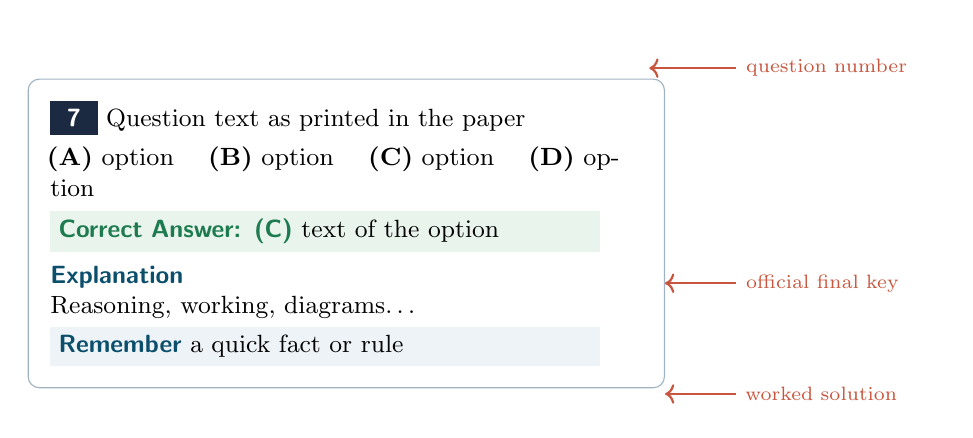
\begin{tikzpicture}[font=\small,every node/.style={align=left}]
\node[draw=rule,rounded corners,fill=white,text width=0.62\linewidth,inner sep=8pt] (q) {%
\colorbox{ink}{\makebox[1.2em]{\sffamily\bfseries\small\color{white}7}}\ Question text as printed in the paper\\[3pt]
\textbf{(A)} option \quad \textbf{(B)} option \quad \textbf{(C)} option \quad \textbf{(D)} option\\[4pt]
\colorbox{softgood}{\parbox{0.9\linewidth}{\sffamily\small\textbf{\color{good}Correct Answer: (C)}\ \rmfamily text of the option}}\\[4pt]
{\sffamily\small\bfseries\color{brand}Explanation}\\ Reasoning, working, diagrams\ldots\\[3pt]
\colorbox{soft}{\parbox{0.9\linewidth}{\sffamily\small\bfseries\color{brand}Remember\ \rmfamily\mdseries\color{black} a quick fact or rule}}};
\draw[<-,accent,thick] ([yshift=18pt]q.north east) ++(-0.2,-0.5) -- ++(1.1,0) node[right,font=\scriptsize,text width=2.4cm]{question number};
\draw[<-,accent,thick] ([yshift=-18pt]q.east) -- ++(0.9,0) node[right,font=\scriptsize,text width=2.4cm]{official final key};
\draw[<-,accent,thick] ([yshift=-58pt]q.east) -- ++(0.9,0) node[right,font=\scriptsize,text width=2.4cm]{worked solution};
\end{tikzpicture}
\end{center}

\section*{Suggested study plan}
\begin{enumerate}
\item \textbf{Attempt first, read later.} Take each paper as a timed test: 50 questions (or 60 in the older papers where 50 were to be answered) in one hour. Mark your answers, then check them against the \emph{Official Final Answer Key} grid at the start of each chapter. Each question number in the grid is a link in the PDF edition.
\item \textbf{Study every explanation}, including those for the questions you got right. Many explanations add the surrounding facts (for example, all SWAYAM national coordinators, all NAAC criteria, or all the Nyaya pramanas), which are exactly what later papers ask.
\item \textbf{Redo the reasoning questions} (series, coding, clocks, dice, Venn diagrams, data interpretation) without looking at the working. These are the scoring questions of Paper~I.
\item \textbf{Keep a mistake log} of topics you get wrong, and revise them with the tips in the grey \emph{Remember} boxes.
\end{enumerate}

\section*{Symbols and conventions}
\begin{tabularx}{\linewidth}{@{}lX@{}}\toprule
\textbf{Mark} & \textbf{Meaning}\\\midrule
\colorbox{softgood}{\sffamily\small\color{good}\textbf{Correct Answer}} & Answer as per the GSET Agency's final key.\\[3pt]
\colorbox{soft}{\sffamily\small\color{accent}\textbf{Dropped question}} & Question marked Z/X in the final key: not evaluated. The most defensible answer is still discussed.\\[3pt]
{\sffamily\small\color{accent}\textbf{Note on the key}} & The official key differs from what the question strictly supports; both are explained.\\[3pt]
Framed box & A reading passage, table or chart shared by a group of questions.\\\bottomrule
\end{tabularx}

\medskip
Diagrams, charts and tables have been \textbf{redrawn} from the original booklets. In a handful of figure-based questions (for example, symbol sequences) the original figure has been reproduced as an image so that nothing is lost.

{\hypersetup{linkcolor=ink}\setcounter{tocdepth}{0}\tableofcontents}
\chapter*{About GSET Paper I}
\addcontentsline{toc}{chapter}{About GSET Paper I}
\markboth{About GSET Paper I}{About GSET Paper I}

\section*{The examination}
The \textbf{Gujarat State Eligibility Test (GSET)} is conducted by the GSET Agency, \textbf{The Maharaja Sayajirao University of Baroda, Vadodara}, as the UGC-accredited State Eligibility Test for Gujarat (and Goa in some years). Qualifying GSET makes a candidate eligible for the post of \textbf{Assistant Professor} in universities and colleges of the State.

\section*{Pattern of Paper I}
\begin{center}\small
\begin{tabularx}{\linewidth}{@{}lX@{}}\toprule
\textbf{Feature} & \textbf{Details}\\\midrule
Nature & General paper on teaching and research aptitude, common to all subjects\\
Questions & 50 compulsory MCQs (2017 and earlier: 60 given, any 50 to be answered, the first 50 attempted being evaluated)\\
Marks & 2 marks each, 100 marks in total; no negative marking\\
Medium & Bilingual question booklet (English and Gujarati)\\
Duration & 1 hour (Paper I, followed by Paper II on the subject)\\\bottomrule
\end{tabularx}
\end{center}

\section*{Syllabus (UGC-aligned units)}
\begin{enumerate}[leftmargin=2em]
\item \textbf{Teaching Aptitude}: concept, objectives, levels of teaching (memory, understanding, reflective); learner characteristics; factors affecting teaching; methods of teaching; teaching support systems; evaluation systems.
\item \textbf{Research Aptitude}: meaning, types and characteristics of research; positivism and post-positivism; methods (experimental, descriptive, historical, qualitative, quantitative); steps; thesis and article writing; research ethics.
\item \textbf{Comprehension}: a passage followed by questions.
\item \textbf{Communication}: meaning, types and characteristics; effective communication; verbal and non-verbal; inter-cultural and group communication; classroom communication; barriers; mass media and society.
\item \textbf{Mathematical Reasoning and Aptitude}: types of reasoning; number, letter and code series; relationships; fractions, time and distance, ratio, proportion, percentages, profit and loss, interest, discounting, averages.
\item \textbf{Logical Reasoning}: structure of arguments; deductive and inductive reasoning; analogies; Venn diagrams; Indian logic (pramanas, anumana, vyapti, hetvabhasa).
\item \textbf{Data Interpretation}: sources, acquisition and classification of data; quantitative and qualitative data; graphical representation (bar chart, histogram, pie chart, table chart, line chart); data and governance.
\item \textbf{Information and Communication Technology (ICT)}: general abbreviations and terminology; basics of the internet, intranet, e-mail, audio and video conferencing; digital initiatives in higher education; ICT and governance.
\item \textbf{People, Development and Environment}: development and environment (MDGs and SDGs); human--environment interaction; environmental issues; pollutants and their impact; natural and energy resources; natural hazards and disasters; environmental protection acts and international agreements.
\item \textbf{Higher Education System}: institutions of learning in ancient India; evolution of higher learning after independence; oriental, conventional and non-conventional learning; professional, technical and skill-based education; value education; policies, governance and administration (including NEP~2020).
\end{enumerate}

\section*{Papers in this book}
\begin{center}\small
\begin{tabular}{llcc}\toprule
\textbf{Examination} & \textbf{Date} & \textbf{Booklet} & \textbf{Questions}\\\midrule
November 2025 & 16 Nov 2025 & A & 50\\ December 2024 & 1 Dec 2024 & A & 50\\ November 2023 & 26 Nov 2023 & A & 50\\ November 2022 & 6 Nov 2022 & A & 50\\ December 2021 & 23 Jan 2022 & A & 50\\ December 2019 & 29 Dec 2019 & A & 50\\ September 2018 & 30 Sep 2018 & A & 50\\ August 2017 & 27 Aug 2017 & A & 60\\ September 2016 & 25 Sep 2016 & A & 60\\ October 2014 & Oct 2014 & A & 60\\ December 2013 & Dec 2013 & A & 60\\ September 2013 & Sep 2013 & A & 60\\ October 2011 & Oct 2011 & A & 60\\ October 2010 & Oct 2010 & A & 60\\ December 2008 & 7 Dec 2008 & C & 50\\ July 2006 & Jul 2006 & A & 50\\ July 2004 & 25 Jul 2004 & C & 50\\ December 2003 & 7 Dec 2003 & C & 50\\ December 2002 & 1 Dec 2002 & B & 50\\ January 2002 & 20 Jan 2002 & B & 50\\\midrule
\textbf{Total} & & & \textbf{1{,}070}\\\bottomrule
\end{tabular}
\end{center}


\mainmatter
\paperchapter{November 2025}{16 November 2025}{A}{50}{19th GSET}
\keytable{\kcell{1}{A} & \kcell{2}{B} & \kcell{3}{D} & \kcell{4}{D} & \kcell{5}{A} & \kcell{6}{C} & \kcell{7}{C} & \kcell{8}{A} & \kcell{9}{A} & \kcell{10}{D} \\
\kcell{11}{A} & \kcell{12}{A} & \kcell{13}{C} & \kcell{14}{B} & \kcell{15}{B} & \kcell{16}{B} & \kcell{17}{B} & \kcell{18}{B} & \kcell{19}{A} & \kcell{20}{C} \\
\kcell{21}{B} & \kcell{22}{C} & \kcell{23}{A} & \kcell{24}{C} & \kcell{25}{C} & \kcell{26}{D} & \kcell{27}{D} & \kcell{28}{C} & \kcell{29}{B} & \kcell{30}{C} \\
\kcell{31}{D} & \kcell{32}{B} & \kcell{33}{C} & \kcell{34}{C} & \kcell{35}{A} & \kcell{36}{C} & \kcell{37}{A} & \kcell{38}{A} & \kcell{39}{D} & \kcell{40}{C} \\
\kcell{41}{C} & \kcell{42}{A} & \kcell{43}{D} & \kcell{44}{A} & \kcell{45}{C} & \kcell{46}{B} & \kcell{47}{B} & \kcell{48}{B} & \kcell{49}{B} & \kcell{50}{C}}
\begin{question}{1}
{Which of the following is an example of synchronous communication in ICT?\par}
\optstwo{Video conferencing}{E-mails}{Blogs}{Wikis}
\answer{A}{Video conferencing}
\begin{explain}
In \textbf{synchronous} communication all participants are present \emph{at the same time} and interact in real time. Video conferencing (Zoom, Google Meet, Microsoft Teams), live chat, telephone calls and live webinars are synchronous.
\why{E-mails, blogs and wikis are \textbf{asynchronous}: the sender writes now and the receiver reads or edits later, at a time of their own choosing.}
\tip{Synchronous = same time (live). Asynchronous = different time (stored and forwarded).}
\end{explain}
\end{question}

\begin{question}{2}
{Who is known as the Inventor of Artificial Intelligence?\par}
\optstwo{Charles Babbage}{John McCarthy}{Andrew Ng}{Mark Zuckerberg}
\answer{B}{John McCarthy}
\begin{explain}
\textbf{John McCarthy} (1927--2011) coined the term \emph{Artificial Intelligence} in the 1955 proposal for the \textbf{Dartmouth Summer Research Project (1956)}, the event regarded as the birth of AI as a field. He also created the \textbf{LISP} programming language (1958), long the main language of AI research.
\why{Charles Babbage designed the Analytical Engine and is called the ``father of the computer''. Andrew Ng is a modern machine-learning researcher (co-founder of Coursera and Google Brain). Mark Zuckerberg founded Facebook.}
\end{explain}
\end{question}

\begin{question}{3}
{Identify the incorrect pair of Swayam Prabha DTH Channel and its theme/subject.\par}
\optsone{Channel 01 VAGEESH : Language and Literature}{Channel 03 PRABODH : Social and Behavioral Science}{Channel 06 VIDHIK : Law, Legal Studies and Human Rights}{Channel 10 DAKSH : Life Sciences}
\answer{D}{Channel 10 DAKSH : Life Sciences}
\begin{explain}
The 40 SWAYAM Prabha DTH channels are each dedicated to a theme. Channel~01 \emph{Vageesh} (Language \& Literature), Channel~03 \emph{Prabodh} (Social \& Behavioural Sciences) and Channel~06 \emph{Vidhik} (Law, Legal Studies \& Human Rights) are correctly matched. Channel~10 \emph{Daksh} is devoted to \emph{Applied Sciences}; Life Sciences is carried by Channel~09 \emph{Spandan}. Hence pair (D) is incorrect.
\tip{SWAYAM Prabha: 40 free 24$\times$7 educational DTH channels via GSAT-15, launched 9 July 2017; content from CEC--UGC, NPTEL (IITs), IGNOU, NCERT, NIOS and others.}
\end{explain}
\end{question}

\begin{question}{4}
{Which of the following softwares are used in India for plagiarism checking?\newline I. Turnitin\newline II. Drill Bit\newline III. Urkund\newline Choose the correct option:\par}
\optstwo{I and II only}{I and III only}{II and III only}{I, II and III}
\answer{D}{I, II and III}
\begin{explain}
All three are plagiarism-detection tools used by Indian institutions:
\begin{itemize}
\item \textbf{Turnitin} -- widely used international service.
\item \textbf{DrillBit} -- Indian-developed software; provided free to universities by the Ministry of Education/INFLIBNET under the \emph{ShodhShuddhi} initiative (from 2022).
\item \textbf{Urkund} (now \emph{Ouriginal}) -- the tool originally supplied by INFLIBNET under ShodhShuddhi (2019).
\end{itemize}
The UGC (Promotion of Academic Integrity and Prevention of Plagiarism in HEIs) Regulations, 2018 require such checks for theses and dissertations. Hence I, II and III.
\end{explain}
\end{question}

\begin{question}{5}
{Put the following units of storage into the correct order, starting with the largest unit first and going down to the smallest unit.\newline i. Kilobyte\newline ii. Byte\newline iii. Megabyte\newline iv. Terabyte\newline v. Gigabyte\newline vi. Bit\newline Choose the correct option:\par}
\optstwo{iv, v, iii, i, ii, vi}{v, iv, iii, i, ii, vi}{iv, iii, v, i, ii, vi}{iv, v, i, ii, iii, vi}
\answer{A}{iv, v, iii, i, ii, vi}
\begin{explain}
Storage units from the largest to the smallest:
\[\text{Terabyte (iv)} > \text{Gigabyte (v)} > \text{Megabyte (iii)} > \text{Kilobyte (i)} > \text{Byte (ii)} > \text{Bit (vi)}\]
(1~TB = 1024~GB, 1~GB = 1024~MB, 1~MB = 1024~KB, 1~KB = 1024~bytes, 1~byte = 8~bits.) The order iv, v, iii, i, ii, vi is option (A).
\end{explain}
\end{question}

\begin{question}{6}
{The encoding of the communication message which takes into consideration the circumstances and environment refers to the\par}
\optsfour{Decoding}{Channel}{Context}{Response}
\answer{C}{Context}
\begin{explain}
\textbf{Context} is the setting (physical, social, cultural, psychological and temporal) in which communication takes place. A sender who encodes a message keeping the circumstances and environment in mind is taking the \emph{context} into account; the same words may carry different meanings in different contexts.
\why{Decoding is the receiver interpreting the message; the channel is the medium that carries it; the response is the receiver's reaction or feedback.}
\end{explain}
\end{question}

\begin{question}{7}
{Two students who stand apart from each other, maintaining their territorial boundaries, refers to\par}
\optsfour{Haptics}{Kinesics}{Proxemics}{Chronemics}
\answer{C}{Proxemics}
\begin{explain}
\textbf{Proxemics} (term coined by Edward T.~Hall, 1966) is the study of how people use \emph{space and distance} in communication: intimate, personal, social and public zones. Students keeping a distance to maintain their ``territory'' is a proxemic behaviour.
\why{Haptics = touch; Kinesics = body movements, gestures and facial expressions; Chronemics = use of time.}
\end{explain}
\end{question}

\begin{question}{8}
{The teachers give regular feedback to their institutional heads on student performance through \blank{} of communication.\par}
\optstwo{Upward channel}{Horizontal channel}{Downward channel}{Lateral channel}
\answer{A}{Upward channel}
\begin{explain}
Communication that flows from subordinates to superiors (teacher $\rightarrow$ head of institution) is \textbf{upward communication}. Reports, feedback, suggestions and grievances travel upward.
\why{Downward flows from superior to subordinate (circulars, instructions); horizontal/lateral flows between people at the same level (teacher to teacher).}
\end{explain}
\end{question}

\begin{question}{9}
{Perception barrier in communication occurs because people perceive the\par}
\optsone{Same phenomena from different frame of reference}{Different phenomena from different frame of reference}{Different phenomena from same frame of reference}{Same phenomena from same frame of reference}
\answer{A}{Same phenomena from different frame of reference}
\begin{explain}
A \textbf{perceptual barrier} arises because different people look at the \emph{same} event, message or phenomenon from \emph{different frames of reference} (their experiences, beliefs, culture and expectations) and therefore interpret it differently.
\tip{Frame of reference = the mental ``lens'' formed by one's background. Same reality + different lenses = different perceptions.}
\end{explain}
\end{question}

\begin{question}{10}
{Yellow journalism is\par}
\optstwo{Development Journalism}{Print Journalism}{Investigative Journalism}{Tabloid Journalism}
\answer{D}{Tabloid Journalism}
\begin{explain}
\textbf{Yellow journalism} is sensational, exaggerated and poorly researched reporting meant to attract readers; the term comes from the 1890s circulation war in New York between Pulitzer's \emph{New York World} and Hearst's \emph{New York Journal}. Its modern form is \textbf{tabloid journalism}.
\why{Development journalism reports on development issues; investigative journalism involves in-depth, fact-based inquiry; print journalism is simply the medium.}
\end{explain}
\end{question}

\begin{question}{11}
{Find the odd one out from the following.\newline 1. Doctor\newline 2. Hospital\newline 3. Nurse\newline 4. Patient\par}
\optsfour{2}{3}{1}{4}
\answer{A}{2}
\begin{explain}
Doctor, Nurse and Patient are all \emph{persons} found in a hospital; \textbf{Hospital} (item~2) is the \emph{place} itself. Hence item~2 is the odd one out, which is option (A).
\end{explain}
\end{question}

\begin{question}{12}
{The abhava of thing is known through\par}
\optsfour{Anupalabdhi}{Arthapalthi}{Upasthiti}{Upalabdhi}
\answer{A}{Anupalabdhi}
\begin{explain}
In Bhatta Mimamsa and Advaita Vedanta, \textbf{Anupalabdhi} (non-perception or non-cognition) is the independent \emph{pramana} (means of valid knowledge) through which the \textbf{abhava} (non-existence or absence) of a thing is known. For example, ``there is no pot on the floor'' is known by the non-perception of a pot where it would have been perceived.
\why{Arthapatti is postulation or presumption (e.g.\ ``fat Devadatta does not eat by day, so he eats at night''). Upalabdhi means perception, which is the opposite. Upasthiti is not a pramana.}
\tip{Six pramanas (Mimamsa/Vedanta): Pratyaksha, Anumana, Upamana, Shabda, Arthapatti, Anupalabdhi.}
\end{explain}
\end{question}

\begin{question}{13}
{What are the missing letters in the following series?\newline pqr \_ \_ rsprs \_ \_ spq \_\par}
\optsfour{pqppq}{spqpr}{sqpqr}{sqprq}
\answer{C}{sqpqr}
\begin{explain}
Fill the blanks with \textbf{s, q, p, q, r}:
\[\text{pqr\underline{s}}\ \ \text{\underline{q}rsp}\ \ \text{rs\underline{p}\underline{q}}\ \ \text{spq\underline{r}}\]
Each block of four letters is the previous block shifted one place to the left (pqrs $\rightarrow$ qrsp $\rightarrow$ rspq $\rightarrow$ spqr). The missing letters are s, q, p, q, r, i.e.\ ``sqpqr'', option (C).
\end{explain}
\end{question}

\begin{question}{14}
{If `ideas' related to `brain', then `money' related to \blank{}.\par}
\optsfour{Cash}{Bank}{Loan}{Investment}
\answer{B}{Bank}
\begin{explain}
The relation is \emph{thing : place where it is stored or kept}. Ideas are stored in the brain; money is kept (deposited) in a bank.
\why{Cash is a form of money, a loan is borrowed money, and an investment is a use of money. None of these is the place where money is kept.}
\end{explain}
\end{question}

\begin{question}{15}
{What is the correct sequence of the five membered syllogism (Avayavas) in the Nyaya System?\par}
\optsone{Hetu -- Pratijna -- Upanaya -- Udharana -- Nigamana}{Pratijna -- Hetu -- Udharana -- Upanaya -- Nigamana}{Udharana -- Hetu -- Upanaya -- Nigamana -- Pratijna}{Pratijna -- Udharana -- Hetu -- Nigamana -- Upanaya}
\answer{B}{Pratijna -- Hetu -- Udharana -- Upanaya -- Nigamana}
\begin{explain}
The \textbf{Nyaya five-membered syllogism (Panchavayava)} in its correct order:
\begin{enumerate}
\item \textbf{Pratijna} (proposition): The hill has fire.
\item \textbf{Hetu} (reason): Because it has smoke.
\item \textbf{Udaharana} (example): Wherever there is smoke there is fire, as in a kitchen.
\item \textbf{Upanaya} (application): The hill has smoke, which is invariably accompanied by fire.
\item \textbf{Nigamana} (conclusion): Therefore the hill has fire.
\end{enumerate}
This is option (B).
\end{explain}
\end{question}

\begin{question}{16}
{Which of the following best defines descriptive research?\par}
\optsone{Research focused solely on creating new theories}{Investigation focused on presenting status of a phenomena as they exist}{Study to prove scientific law under controlled situation}{Research designed to change existing conditions}
\answer{B}{Investigation focused on presenting status of a phenomena as they exist}
\begin{explain}
\textbf{Descriptive research} describes ``what is'', meaning the current status of a phenomenon as it naturally exists, without manipulating variables. Surveys, case studies, developmental and correlational studies are descriptive.
\why{Creating new theory is the aim of fundamental or grounded-theory research; proving laws under controlled conditions is experimental research; changing existing conditions is the aim of action research.}
\end{explain}
\end{question}

\begin{question}{17}
{An opinionnaire based study on social issues will have\par}
\optstwo{Historical method}{Survey method}{Experimental method}{Quantitative method}
\answer{B}{Survey method}
\begin{explain}
An \textbf{opinionnaire} (attitude scale or opinion questionnaire) collects the opinions of a large number of respondents on social issues. Collecting such data from a sample to describe a population is the \textbf{survey method}, a form of descriptive research.
\why{The historical method studies past records; the experimental method manipulates variables; ``quantitative'' is a type of data or approach, not a specific method of this kind.}
\end{explain}
\end{question}

\begin{question}{18}
{What is an ethically appropriate method when referring to individual participants in research?\par}
\optsone{List all their names with their responses}{Use code language or anonymous identifiers}{Ask participants to publish their own data}{Replace names with name of data collectors}
\answer{B}{Use code language or anonymous identifiers}
\begin{explain}
Research ethics require \textbf{confidentiality and anonymity}: participants should be referred to by codes, pseudonyms or anonymous identifiers (e.g.\ Respondent R-12, Teacher T3) so that responses cannot be traced back to individuals.
\why{Listing names with responses violates confidentiality; asking participants to publish their own data is irrelevant; replacing names with those of the data collectors is misleading.}
\end{explain}
\end{question}

\begin{question}{19}
{Which of the following set has only qualitative measurement?\par}
\optstwo{Values, attitude, anecdotes}{Capital investment, vision, mission}{Values, performance, profit}{Expenditure, investment, profit}
\answer{A}{Values, attitude, anecdotes}
\begin{explain}
Qualitative measurement deals with \emph{non-numerical} attributes. \textbf{Values, attitudes and anecdotes} are all qualitative, described in words, categories or ratings of quality.
\why{Every other set contains quantitative items: capital investment, profit, performance scores and expenditure are measured in numbers.}
\end{explain}
\end{question}

\begin{question}{20}
{What percentage of observations are broadly covered from `0' SD to `-3' SD of normal probability distribution curve?\par}
\optsfour{100\%}{0\%}{50\%}{30\%}
\answer{C}{50\%}
\begin{explain}
The normal curve is symmetric about the mean (0~SD), so exactly half the observations lie on each side. The area from the mean to $-3\,\sigma$ is 49.87\%, which is broadly \textbf{50\%}.
\begin{center}
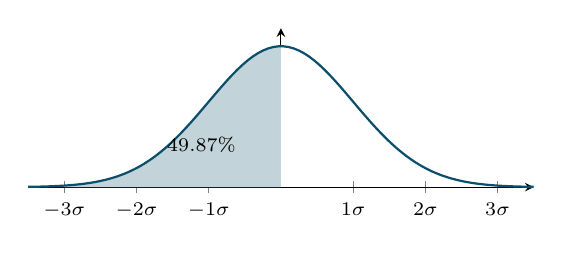
\begin{tikzpicture}
\begin{axis}[width=8cm,height=3.6cm,axis lines=middle,ytick=\empty,xtick={-3,-2,-1,0,1,2,3},
  xticklabels={$-3\sigma$,$-2\sigma$,$-1\sigma$,$0$,$1\sigma$,$2\sigma$,$3\sigma$},
  ymin=0,ymax=0.45,xmin=-3.5,xmax=3.5,tick label style={font=\scriptsize}]
\addplot[domain=-3:0,samples=60,fill=brand!25,draw=none] {exp(-x^2/2)/sqrt(2*pi)} \closedcycle;
\addplot[domain=-3.5:3.5,samples=100,thick,brand] {exp(-x^2/2)/sqrt(2*pi)};
\node[font=\scriptsize] at (axis cs:-1.1,0.12) {49.87\%};
\end{axis}
\end{tikzpicture}
\end{center}
\tip{Mean to $\pm1\sigma$: 34.13\% each side (68.26\% total); $\pm2\sigma$: 95.44\%; $\pm3\sigma$: 99.73\%.}
\end{explain}
\end{question}

\begin{question}{21}
{`Gujarat Public Universities Bill' was passed in Gujarat Legislative Assembly in the year\par}
\optsfour{2022}{2023}{2020}{2021}
\answer{B}{2023}
\begin{explain}
The \textbf{Gujarat Public Universities Bill, 2023} was passed by the Gujarat Legislative Assembly in \textbf{September 2023} and became the \emph{Gujarat Public Universities Act, 2023}. It brings 11 state public universities (e.g.\ Gujarat University, M.S.~University of Baroda, Saurashtra University) under a common Act, replacing their separate Acts, with a Board of Management and a Chancellor appointed by the State.
\end{explain}
\end{question}

\begin{question}{22}
{The primary focus of the National Education Policy -- 2020 is\par}
\optsone{Creating an expensive education system}{Providing free education for all}{Transforming India into a knowledge based society and economy}{Emphasizing traditional education}
\answer{C}{Transforming India into a knowledge based society and economy}
\begin{explain}
NEP~2020 states its vision as an India-centred education system that contributes directly to \textbf{transforming India into an equitable and vibrant knowledge society}, by providing high-quality education to all and making India a global knowledge superpower.
\why{It does not seek an expensive system; ``free education for all'' is not its primary focus (RTE already covers ages 6--14); it blends traditional knowledge with modern education rather than emphasising only tradition.}
\end{explain}
\end{question}

\begin{question}{23}
{Name the parent/route organization for DTH Channel 7 (Kautilya) of Swayam Prabha managed by CEC-UGC, New Delhi.\par}
\optstwo{Gujarat University, EMRC, Ahmedabad}{Punjabi University, EMRC, Patiala}{Calicut University, EMRC, Calicut}{IIT, Delhi}
\answer{A}{Gujarat University, EMRC, Ahmedabad}
\begin{explain}
SWAYAM Prabha channels are produced by partner institutions. Channels coordinated by CEC--UGC are prepared through its \textbf{Educational Multimedia Research Centres (EMRCs)}. Channel~7 (\emph{Kautilya}) is handled by the \textbf{EMRC, Gujarat University, Ahmedabad}.
\tip{CEC (Consortium for Educational Communication) is an inter-university centre of UGC with a network of about 21 EMRCs/AVRCs across India.}
\end{explain}
\end{question}

\begin{question}{24}
{Which University in India is offering the largest number of courses through distance mode?\par}
\optsone{University of Mumbai}{University of Delhi}{Indira Gandhi National Open University, Delhi}{Baba Saheb Ambedkar Open University, Ahmedabad}
\answer{C}{Indira Gandhi National Open University, Delhi}
\begin{explain}
\textbf{IGNOU}, the Indira Gandhi National Open University (est.~1985, New Delhi), is a central open university and the largest in the world by enrolment. It offers the largest number of programmes (over 200) through Open and Distance Learning. It also serves as the national apex body for ODL.
\why{Mumbai and Delhi universities offer distance courses through their distance-education wings, but far fewer. BAOU is Gujarat's state open university.}
\end{explain}
\end{question}

\begin{question}{25}
{Which of the following is a common entrance exam for admission to Medical College in India?\par}
\optsfour{JEE}{CAT}{NEET}{GATE}
\answer{C}{NEET}
\begin{explain}
\textbf{NEET-UG} (National Eligibility-cum-Entrance Test), conducted by the \textbf{National Testing Agency (NTA)}, is the single common entrance examination for MBBS, BDS and AYUSH courses in India.
\why{JEE is for engineering (IITs/NITs); CAT is for management (IIMs); GATE is for postgraduate engineering admissions and PSU recruitment.}
\end{explain}
\end{question}

\begin{question}{26}
{The data on the sales of cellular phones (in '000 Rs.) during 2017 -- 2022 years are 48, 40, 30, 25, 28, 40, respectively. The two years between which the rate of change of sales of cellular phones has been minimum are\par}
\optsfour{2017 -- 2018}{2018 -- 2019}{2019 -- 2020}{2020 -- 2021}
\answer{D}{2020 -- 2021}
\begin{explain}
Year-to-year changes in sales:
\begin{center}\small
\begin{tabular}{lccc}\toprule
Period & From $\rightarrow$ To & Change & \% change\\\midrule
2017--18 & 48 $\rightarrow$ 40 & $-8$ & $-16.7\%$\\
2018--19 & 40 $\rightarrow$ 30 & $-10$ & $-25.0\%$\\
2019--20 & 30 $\rightarrow$ 25 & $-5$ & $-16.7\%$\\
\textbf{2020--21} & \textbf{25 $\rightarrow$ 28} & $\mathbf{+3}$ & $\mathbf{+12.0\%}$\\
2021--22 & 28 $\rightarrow$ 40 & $+12$ & $+42.9\%$\\\bottomrule
\end{tabular}
\end{center}
The smallest change, in both absolute and percentage terms, is between \textbf{2020 and 2021}.
\end{explain}
\end{question}

\begin{question}{27}
{The number of candidates (in lakhs) appearing in an entrance examination from five different locations along with the ratio of passing and failing is given as follows.\par}
\qfigure{\begin{tabular}{ccc}\toprule
\textbf{Location} & \textbf{Candidates (lakh)} & \textbf{Pass : Fail}\\\midrule
P & 1.25 & 7 : 3\\ Q & 3.14 & 5 : 3\\ R & 1.08 & 4 : 5\\ S & 2.27 & 1 : 3\\ T & 1.85 & 3 : 2\\\bottomrule
\end{tabular}}
What is the ratio of the number of candidates failing the exam from location S to that of those failing the exam from location P?
\optsfour{50 : 227}{42 : 289}{289 : 42}{227 : 50}
\answer{D}{227 : 50}
\begin{explain}
Failed from S $= 2.27 \times \dfrac{3}{1+3} = 2.27\times\dfrac34 = 1.7025$ lakh.\\
Failed from P $= 1.25 \times \dfrac{3}{7+3} = 1.25\times\dfrac{3}{10} = 0.375$ lakh.
\[\frac{1.7025}{0.375} = \frac{2.27\times 3/4}{1.25\times 3/10} = \frac{2.27\times 10}{1.25\times 4} = \frac{22.7}{5} = \frac{227}{50}\]
Ratio S : P $=$ \textbf{227 : 50}.
\end{explain}
\end{question}

\begin{question}{28}
{The chance that doctor A will diagnose a disease X correctly is 60 percent. The chance that a patient will die by his treatment after correct diagnosis is 40 percent, and the chance of death by wrong diagnosis is 70 percent. A patient of doctor A, who had disease X died. What is the probability that his disease was diagnosed correctly?\par}
\optsfour{0.28}{0.39}{0.46}{0.52}
\answer{C}{0.46}
\begin{explain}
This is Bayes' theorem. Let $C$ = correct diagnosis and $D$ = death.
\[P(C)=0.6,\quad P(D\,|\,C)=0.4;\qquad P(\bar C)=0.4,\quad P(D\,|\,\bar C)=0.7\]
\[P(C\,|\,D)=\frac{0.6\times0.4}{0.6\times0.4+0.4\times0.7}=\frac{0.24}{0.24+0.28}=\frac{0.24}{0.52}\approx \mathbf{0.46}\]
\begin{center}

\begin{tikzpicture}[font=\scriptsize,>=Stealth,node distance=4mm]
\node (p) {Patient with X};
\node (c) at (3,0.6) {Correct (0.6)}; \node (w) at (3,-0.6) {Wrong (0.4)};
\node (cd) at (6.2,0.6) {Dies (0.4): $0.24$}; \node (wd) at (6.2,-0.6) {Dies (0.7): $0.28$};
\draw[->] (p.east) -- (c.west); \draw[->] (p.east) -- (w.west);
\draw[->] (c) -- (cd); \draw[->] (w) -- (wd);
\end{tikzpicture}
\end{center}
\end{explain}
\end{question}

\begin{question}{29}
{The probability that a student is not a swimmer is 1/5. Out of 5 students, what is the probability that atleast 4 are swimmers?\par}
\optsfour{0.65}{0.74}{0.79}{0.82}
\answer{B}{0.74}
\begin{explain}
$P(\text{not swimmer})=\tfrac15 \Rightarrow p=P(\text{swimmer})=\tfrac45=0.8,\ q=0.2$, $n=5$ (binomial).
\[P(X\ge4)=\binom54(0.8)^4(0.2)+\binom55(0.8)^5=5(0.4096)(0.2)+0.32768=0.4096+0.32768=0.73728\]
$\approx$ \textbf{0.74}.
\end{explain}
\end{question}

\begin{question}{30}
{Some tickets are numbered from 1, 2, \ldots{}, 100 for a random draw. What is the probability that the number drawn is a multiple of 3 or 5?\par}
\optsfour{0.27}{0.37}{0.47}{0.57}
\answer{C}{0.47}
\begin{explain}
Multiples of 3 in 1--100: $\lfloor100/3\rfloor=33$. Multiples of 5: $20$. Multiples of both (i.e.\ of 15): $6$.
\[n(3\cup5)=33+20-6=47\qquad\Rightarrow\qquad P=\frac{47}{100}=\mathbf{0.47}\]
\end{explain}
\end{question}

\begin{question}{31}
{Which of the following is not a state of memory level?\par}
\optsfour{Retention}{Recall}{Recognition}{Assimilation}
\answer{D}{Assimilation}
\begin{explain}
Memory is studied through the processes of \textbf{encoding/learning, retention (storage), recall and recognition}, and these are the recognised states or levels at which memory is measured. \textbf{Assimilation} is a Piagetian concept of \emph{cognitive development} (fitting new experience into existing schemas). It is not a state of memory.
\end{explain}
\end{question}

\begin{question}{32}
{For teachers, it is important to consider the individual differences amongst learners. This helps to\par}
\optsone{Classify the students in to subgroups for different activities}{Guide learning and develop students' cognitive processes}{Ensure uniform teaching for all students}{Reduce the need for assessment}
\answer{B}{Guide learning and develop students' cognitive processes}
\begin{explain}
Recognising individual differences (in ability, pace, learning style, interest and background) lets a teacher \textbf{guide learning} appropriately and \textbf{develop each student's cognitive processes} through differentiated instruction.
\why{Classifying students into subgroups is at best a tool, not the purpose; uniform teaching ignores differences; individual differences do not reduce the need for assessment.}
\end{explain}
\end{question}

\begin{question}{33}
{Which of the following is most significant for student learning?\par}
\optstwo{Student background}{Prior academic achievement}{Active learning processes}{Availability of textbooks}
\answer{C}{Active learning processes}
\begin{explain}
Modern learning theory (constructivism) holds that learning happens when learners \textbf{actively} construct knowledge by doing, discussing, questioning and reflecting. Active learning processes therefore matter most, while background, prior achievement and textbooks are supporting factors.
\end{explain}
\end{question}

\begin{question}{34}
{What type of content is broadcast on the Swayam Prabha Channel?\par}
\optsone{Weather and entertainment programmes}{Political debate programmes}{Educational programmes covering diverse fields for the 18+ age group learners}{Telecast of job opportunities to apply}
\answer{C}{Educational programmes covering diverse fields for the 18+ age group learners}
\begin{explain}
SWAYAM Prabha telecasts high-quality \textbf{educational programmes in diverse disciplines} (arts, science, commerce, engineering, social sciences, law, medicine, agriculture and more) for school, higher-education and lifelong learners. For the higher-education channels the target group is learners aged roughly 18 and above.
\end{explain}
\end{question}

\begin{question}{35}
{Under CBCS system, the requirement for awarding degree is determined by\par}
\optsone{Number of credits earned by the students}{Number of years spent in the programme}{Marks obtained in semester examination}{Attendance and Internal Assessment (IA) marks only}
\answer{A}{Number of credits earned by the students}
\begin{explain}
Under the \textbf{Choice Based Credit System (CBCS)}, introduced by UGC in 2015, each course carries credits, and a degree is awarded when the student earns the \textbf{prescribed minimum number of credits} across core, elective and ability- or skill-enhancement courses. Grades are expressed as SGPA/CGPA.
\why{Years of study, raw marks or attendance alone do not decide the award of the degree under CBCS.}
\end{explain}
\end{question}

\begin{question}{36}
{`Fly ash' produced in thermal power plant is useful in\newline i. Road construction\newline ii. Wasteland development\newline iii. Agriculture as micro-nutrient\newline iv. Brick making\newline Choose the correct option:\par}
\optstwo{i, ii and iii only}{ii, iii and iv only}{i, ii, iii and iv}{i, ii and iv only}
\answer{C}{i, ii, iii and iv}
\begin{explain}
Fly ash, the fine residue of coal combustion, is used for:
\begin{itemize}
\item \textbf{road and embankment construction} (the MoRTH/IRC encourage its use);
\item \textbf{wasteland reclamation and development};
\item \textbf{agriculture}, as a soil conditioner supplying micro-nutrients (B, Mo, Zn, S) and improving water-holding capacity;
\item \textbf{brick making}: fly-ash bricks are mandated near thermal power plants by the MoEF notification of 1999.
\end{itemize}
All four uses are correct, so the answer is (C).
\end{explain}
\end{question}

\begin{question}{37}
{Arrange the following themes of Sustainable Development Goals according to their goal number in decreasing order.\newline I. Life below water\newline II. Clean water and sanitation\newline III. Life on land\newline IV. Climate action\newline V. Affordable and clean energy\newline Choose the correct option:\par}
\optstwo{III, I, IV, V, II}{III, I, V, IV, II}{III, I, II, IV, V}{III, I, IV, II, V}
\answer{A}{III, I, IV, V, II}
\begin{explain}
SDG numbers: Life on land = \textbf{15}, Life below water = \textbf{14}, Climate action = \textbf{13}, Affordable and clean energy = \textbf{7}, Clean water and sanitation = \textbf{6}.
Decreasing order: 15 (III), 14 (I), 13 (IV), 7 (V), 6 (II), giving \textbf{III, I, IV, V, II}.
\tip{SDGs 6--7--13--14--15 = Water, Energy, Climate, Oceans, Land.}
\end{explain}
\end{question}

\begin{question}{38}
{Given below are two statements.\newline Statement -- I : Cyclones developed in the region lying between the Tropic of Capricorn and Cancer are called tropical cyclones.\newline Statement -- II : Hurricane Helene was a large, catastrophic and deadly tropical cyclone that caused widespread destruction and fatalities across the South-Eastern United States in September 2024.\newline In light of the above statements, choose the correct answer from the options given below:\par}
\optsone{Both Statement -- I and Statement -- II are true}{Both Statement -- I and Statement -- II are false}{Statement -- I is true, but Statement -- II is false}{Statement -- I is false, but Statement -- II is true}
\answer{A}{Both Statement -- I and Statement -- II are true}
\begin{explain}
\textbf{Statement I} is true: cyclones that originate over warm tropical oceans, in the belt between the Tropic of Cancer and the Tropic of Capricorn, are called tropical cyclones (hurricanes, typhoons and so on).
\textbf{Statement II} is true: Hurricane Helene (late September 2024) made landfall in Florida's Big Bend as a Category~4 storm and caused catastrophic flooding and more than 200 deaths across the south-eastern US, especially North Carolina.
Both statements are true, so the answer is (A).
\end{explain}
\end{question}

\begin{question}{39}
{How many States in India are identified as highly vulnerable to climate change as per the National Climate Vulnerability Assessment Report by the Department of Science and Technology, Govt. of India (2024)?\par}
\optsfour{5}{6}{7}{8}
\answer{D}{8}
\begin{explain}
The Department of Science \& Technology's national report \emph{Climate Vulnerability Assessment for Adaptation Planning in India using a Common Framework} identified \textbf{eight} eastern and north-eastern states as highly vulnerable: Jharkhand, Mizoram, Odisha, Chhattisgarh, Assam, Bihar, Arunachal Pradesh and West Bengal.
\end{explain}
\end{question}

\begin{question}{40}
{Which of the following oxides of Nitrogen is a constituent of Air Quality Index?\par}
\optstwo{Nitric Oxide (NO)}{Nitrous Oxide (N$_2$O)}{Nitrogen Dioxide (NO$_2$)}{Dinitrogen Tetroxide (N$_2$O$_4$)}
\answer{C}{Nitrogen Dioxide (NO$_2$)}
\begin{explain}
India's \textbf{National Air Quality Index} (launched 2014) uses eight pollutants: PM$_{10}$, PM$_{2.5}$, \textbf{NO$_2$}, SO$_2$, CO, O$_3$, NH$_3$ and Pb. Of the nitrogen oxides, only \textbf{nitrogen dioxide} is an AQI constituent.
\tip{AQI categories: Good (0--50), Satisfactory (51--100), Moderately polluted (101--200), Poor (201--300), Very poor (301--400), Severe (401--500).}
\end{explain}
\end{question}

\begin{question}{41}
{If the first and second letter in the word `COMMUNICATIONS' were interchanged, also the third and the fourth letters, the fifth and the sixth letters and so on, which letter would be the tenth letter counting from your right?\par}
\optsfour{A}{T}{N}{U}
\answer{C}{N}
\begin{explain}
COMMUNICATIONS has 14 letters. Swap each pair:
\begin{center}\ttfamily
\begin{tabular}{*{14}{c}}
C&O&M&M&U&N&I&C&A&T&I&O&N&S\\
O&C&M&M&N&U&C&I&T&A&O&I&S&N\\
\end{tabular}
\end{center}
10th from the right = $(14-10+1)$ = 5th from the left = \textbf{N}.
\end{explain}
\end{question}

\begin{question}{42}
{The angle A of a triangle ABC is equal to the sum of the two other angles. Also the ratio of the angle B to angle C is 4 : 5. The three angles are\par}
\optsfour{90\textdegree{}, 40\textdegree{}, 50\textdegree{}}{90\textdegree{}, 55\textdegree{}, 35\textdegree{}}{90\textdegree{}, 60\textdegree{}, 30\textdegree{}}{90\textdegree{}, 70\textdegree{}, 20\textdegree{}}
\answer{A}{90\textdegree{}, 40\textdegree{}, 50\textdegree{}}
\begin{explain}
$A=B+C$ and $A+B+C=180^\circ \Rightarrow 2A=180^\circ \Rightarrow A=90^\circ$, so $B+C=90^\circ$.
With $B:C=4:5$: $B=\tfrac49\times90^\circ=40^\circ$, $C=\tfrac59\times90^\circ=50^\circ$. The angles are \textbf{90\textdegree, 40\textdegree, 50\textdegree}.
\end{explain}
\end{question}

\begin{question}{43}
{Find the missing number (?) in the following series.\newline 4, 8, 12, 24, 36, 72, (?)\par}
\optsfour{92}{96}{98}{108}
\answer{D}{108}
\begin{explain}
The series alternately multiplies by 2 and by 1.5:
\[4\xrightarrow{\times2}8\xrightarrow{\times1.5}12\xrightarrow{\times2}24\xrightarrow{\times1.5}36\xrightarrow{\times2}72\xrightarrow{\times1.5}\mathbf{108}\]
(Equivalently, the differences run $+4,+4,+12,+12,+36,+36$.)
\end{explain}
\end{question}

\begin{question}{44}
{The monthly income of a person was Rs. 13,500 and his monthly expenditure was Rs. 9,000. Next year, his income increased by 14\% and his expenditure by 7\%. Find the percentage increase in his savings.\par}
\optsfour{28\%}{30\%}{32\%}{34\%}
\answer{A}{28\%}
\begin{explain}
Original saving $=13{,}500-9{,}000=4{,}500$.\\
New income $=13{,}500\times1.14=15{,}390$; new expenditure $=9{,}000\times1.07=9{,}630$.\\
New saving $=15{,}390-9{,}630=5{,}760$.
\[\text{Increase}=\frac{5{,}760-4{,}500}{4{,}500}\times100=\frac{1{,}260}{4{,}500}\times100=\mathbf{28\%}\]
\end{explain}
\end{question}

\begin{question}{45}
{Find the compound interest on Rs. 1,000 at the rate of 10\% per annum for 18 months when interest is compounded half-yearly.\par}
\optsfour{Rs. 145.25}{Rs. 152.75}{Rs. 157.63}{Rs. 161.49}
\answer{C}{Rs. 157.63}
\begin{explain}
Half-yearly compounding: rate $=10/2=5\%$ per half-year, periods $=18$ months $\div 6 = 3$.
\[A=1000(1.05)^3=1000\times1.157625=1157.63\qquad CI=1157.63-1000=\textbf{Rs.\ 157.63}\]
\end{explain}
\end{question}

\begin{context}
\textbf{Directions for Q.~46 to 50:} Read the following paragraph and answer the questions that follow.\par\smallskip
Effective learning requires a comprehensive approach that involves appropriate curriculum, engaging pedagogy, continuous formative assessment, and adequate student support. The curriculum must be interesting and relevant, and updated regularly to align with the latest knowledge requirements and to meet specified learning outcomes. High-quality pedagogy is then necessary to successfully impart the curricular material to students; pedagogical practices determine the learning experiences that are provided to students, thus directly influencing learning outcomes. The assessment methods must be scientific, designed to continuously improve learning and test the application of knowledge.

To promote creativity, institutions and faculty will have the autonomy to innovate on matters of curriculum, pedagogy, and assessment within a broad framework of higher education qualifications that ensures consistency across institutions and programmes and across the ODL, online, and traditional `in-class' modes. All assessment systems shall also be decided by the HEI, including those that lead to final certification. The Choice Based Credit System (CBCS) will be revised for instilling innovation and flexibility. HEIs shall move to a criterion-based grading system that assesses student's achievement based on the learning goals for each programme, making the system fairer and outcomes more comparable.
\end{context}
\begin{question}{46}
{What are the essential components of effective learning?\par}
\optsone{Curriculum, textbooks, examination and evaluation}{Curriculum, pedagogy, assessment and student support}{Teachers, pedagogy, technology and curricular material}{Student support, knowledge application, assessment and syllabus}
\answer{B}{Curriculum, pedagogy, assessment and student support}
\begin{explain}
The opening sentence lists the four components: ``appropriate \textbf{curriculum}, engaging \textbf{pedagogy}, continuous formative \textbf{assessment}, and adequate \textbf{student support}.''
(This passage is taken from NEP~2020, paragraph~12.1.)
\end{explain}
\end{question}

\begin{question}{47}
{How do pedagogical practices influence students?\par}
\optsone{Enhance grades}{Influence learning experiences and outcomes}{Reduce homework}{Improve classroom interactions}
\answer{B}{Influence learning experiences and outcomes}
\begin{explain}
The passage says pedagogical practices ``determine the \textbf{learning experiences} that are provided to students, thus directly influencing \textbf{learning outcomes}.''
\why{Grades, homework and classroom interaction are not what the passage names.}
\end{explain}
\end{question}

\begin{question}{48}
{What type of autonomy will institutions and faculty have to promote creativity?\par}
\optsone{Autonomy in determining student fees}{Autonomy in curriculum, pedagogy and assessment}{Autonomy in teacher recruitment}{Autonomy in time-table planning}
\answer{B}{Autonomy in curriculum, pedagogy and assessment}
\begin{explain}
``To promote creativity, institutions and faculty will have the autonomy to innovate on matters of \textbf{curriculum, pedagogy, and assessment}.''
\end{explain}
\end{question}

\begin{question}{49}
{What will the revised Choice Based Credit System (CBCS) aim to achieve?\par}
\optstwo{Simplify exams}{Encourage innovation}{Shorten the academic year}{Reduce the number of courses}
\answer{B}{Encourage innovation}
\begin{explain}
``The Choice Based Credit System (CBCS) will be revised for instilling \textbf{innovation} and flexibility.''
\end{explain}
\end{question}

\begin{question}{50}
{What grading system will HEIs adopt for final certification?\par}
\optstwo{Percentage based}{Rank based}{Criterion based}{Time based}
\answer{C}{Criterion based}
\begin{explain}
``HEIs shall move to a \textbf{criterion-based grading system} that assesses student's achievement based on the learning goals for each programme.'' Criterion-referenced grading measures attainment against fixed learning goals rather than against other students (norm-referenced grading).
\end{explain}
\end{question}

\paperchapter{December 2024}{1 December 2024}{A}{50}{18th GSET}
\keytable{\kcell{1}{A} & \kcell{2}{C} & \kcell{3}{A} & \kcell{4}{D} & \kcell{5}{A} & \kcell{6}{B} & \kcell{7}{A} & \kcell{8}{B} & \kcell{9}{A} & \kcell{10}{A} \\
\kcell{11}{A} & \kcell{12}{D} & \kcell{13}{C} & \kcell{14}{D} & \kcell{15}{D} & \kcell{16}{B} & \kcell{17}{B} & \kcell{18}{B} & \kcell{19}{D} & \kcell{20}{B} \\
\kcell{21}{A} & \kcell{22}{B} & \kcell{23}{B} & \kcell{24}{B} & \kcell{25}{A} & \kcell{26}{D} & \kcell{27}{A} & \kcell{28}{A} & \kcell{29}{D} & \kcell{30}{A} \\
\kcell{31}{C} & \kcell{32}{A} & \kcell{33}{B} & \kcell{34}{A} & \kcell{35}{B} & \kcell{36}{A} & \kcell{37}{A} & \kcell{38}{C} & \kcell{39}{B} & \kcell{40}{D} \\
\kcell{41}{B} & \kcell{42}{C} & \kcell{43}{C} & \kcell{44}{B} & \kcell{45}{B} & \kcell{46}{C} & \kcell{47}{B} & \kcell{48}{D} & \kcell{49}{B} & \kcell{50}{C}}
\begin{question}{1}
{Semantic barrier in communication is\par}
\optstwo{Use of technical/difficult language}{Use of technology}{Lack of attention}{Lack of co-ordination}
\answer{A}{Use of technical/difficult language}
\begin{explain}
A \textbf{semantic barrier} arises from problems of \emph{meaning}: words, symbols, jargon or technical terms that the receiver does not understand, or understands differently. Using technical or difficult language is the classic example.
\why{Use of technology relates to channel or technological barriers; lack of attention is a psychological barrier; lack of co-ordination is an organisational barrier.}
\end{explain}
\end{question}

\begin{question}{2}
{The key purpose of effective communication is\par}
\optstwo{Create barriers}{Promote misunderstanding}{Effect change}{Confuse audience}
\answer{C}{Effect change}
\begin{explain}
Communication is purposeful: it aims to inform, persuade, motivate and so \textbf{bring about a change} in the knowledge, attitude or behaviour of the receiver. Effective communication achieves the intended effect.
\why{Barriers, misunderstanding and confusion are the \emph{opposite} of effective communication.}
\end{explain}
\end{question}

\begin{question}{3}
{Identify the correct sequence of the elements in the communication system.\newline a. Speech\newline b. Speaker\newline c. Receiver\newline d. Effect\newline The correct choice is :\par}
\optsfour{b, a, c, d}{a, b, d, c}{b, a, d, c}{c, d, b, a}
\answer{A}{b, a, c, d}
\begin{explain}
In \textbf{Aristotle's model} of communication (the earliest linear model) the elements occur in this order:
\begin{center}
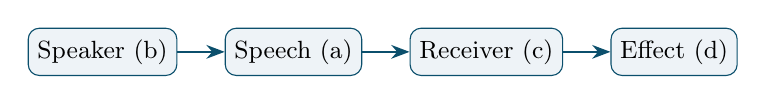
\begin{tikzpicture}[node distance=6mm,every node/.style={draw=brand,rounded corners,fill=soft,font=\small,minimum height=6mm}]
\node (a) {Speaker (b)}; \node[right=of a] (b) {Speech (a)}; \node[right=of b] (c) {Receiver (c)}; \node[right=of c] (d) {Effect (d)};
\draw[-Stealth,thick,brand] (a)--(b); \draw[-Stealth,thick,brand] (b)--(c); \draw[-Stealth,thick,brand] (c)--(d);
\end{tikzpicture}
\end{center}
Speaker $\rightarrow$ Speech $\rightarrow$ Audience (receiver) $\rightarrow$ Effect, i.e.\ \textbf{b, a, c, d}. (Lasswell's later model follows the same logic: \emph{Who says What, in Which channel, to Whom, with What effect}.)
\end{explain}
\end{question}

\begin{question}{4}
{Which of the following is an example of non-verbal communication ?\par}
\optstwo{Writing on the blackboard}{Speaking on microphone}{Sending a voice message}{Nodding head to indicate disagreement}
\answer{D}{Nodding head to indicate disagreement}
\begin{explain}
\textbf{Non-verbal} communication uses no words: gestures, facial expressions, posture, eye contact, head movements, touch, space and time. \textbf{Nodding the head} (to agree or disagree) is a gesture, which falls under kinesics.
\why{Writing on the blackboard is written verbal communication; speaking on a microphone and sending a voice message are oral verbal communication.}
\end{explain}
\end{question}

\begin{question}{5}
{'Encoding' in the communication system means\par}
\optsone{Converting thoughts or ideas into a message}{Translating messages into ideas or thoughts}{Providing opinions on the sender}{Avoiding difficult words in the message}
\answer{A}{Converting thoughts or ideas into a message}
\begin{explain}
\textbf{Encoding} is the sender's act of converting thoughts, ideas or feelings into a message using symbols (words, pictures, gestures).
\why{Option (B) describes \emph{decoding}, which is done by the receiver.}
\end{explain}
\end{question}

\begin{question}{6}
{Which one among the following is the common language for AI ?\par}
\optsfour{Lisp}{Python}{PHP}{JAVA}
\answer{B}{Python}
\begin{explain}
\textbf{Python} is the most widely used language in present-day AI and machine learning, thanks to libraries such as TensorFlow, PyTorch, scikit-learn, NumPy and Keras. The key treats it as the common language for AI.
\why{LISP (1958) was the historical language of AI research, but today it is niche. PHP is a web scripting language, and Java, though usable, is not the common AI language.}
\end{explain}
\end{question}

\begin{question}{7}
{Regarding ICT based governance, which of the following statements is/are correct?\newline i. Increasing transparency is an advantage of ICT based governance.\newline ii. e-governance is related to automation of administrative processes.\newline iii. Due to ICT based governance, workforce gets reduced.\newline Choose the correct option:\par}
\optstwo{i, ii and iii}{i and ii only}{i and iii only}{ii and iii only}
\answer{A}{i, ii and iii}
\begin{explain}
All three statements are correct:
\begin{itemize}
\item ICT increases \textbf{transparency} (online records, RTI portals, e-tendering).
\item e-Governance involves \textbf{automation of administrative processes} (e-office, online services).
\item Automation reduces paperwork and manual jobs, so the \textbf{workforce needed is reduced}.
\end{itemize}
Hence i, ii and iii.
\end{explain}
\end{question}

\begin{question}{8}
{Which among the following are the National Co-ordinators for SWAYAM?\newline 1. Indian Institute of Technology Kanpur (IITK)\newline 2. University Grants Commission (UGC)\newline 3. Consortium for Educational Communication (CEC)\newline 4. Indian Institute of Management Bangalore (IIMB)\newline 5. National Institute of Open Schooling (NIOS)\newline Choose the correct answer from the options given below :\par}
\optsfour{1, 2, 3 and 4}{2, 3, 4 and 5}{1, 2, 3 and 5}{2, 3 and 4}
\answer{B}{2, 3, 4 and 5}
\begin{explain}
SWAYAM has \textbf{nine National Coordinators}, each responsible for one type of content: AICTE (self-paced and international courses), \textbf{NPTEL/IIT Madras} (engineering), \textbf{UGC} (non-technical postgraduate education), \textbf{CEC} (undergraduate education), \textbf{NCERT} and \textbf{NIOS} (school education), IGNOU (out-of-school students), \textbf{IIM Bangalore} (management studies) and NITTTR (teacher training).
Among the given names, UGC, CEC, IIMB and NIOS are national coordinators. IIT Kanpur is not (NPTEL is coordinated through IIT Madras), so the answer is \textbf{2, 3, 4 and 5}.
\end{explain}
\end{question}

\begin{question}{9}
{Given below are two statements:\newline Statement I: SWAYAM is India's own MOOC platform, which offers free online courses in almost all the discipline to students/learners.\newline Statement - II: Coursera, Udemy, Udacity, Iversity are other MOOC platforms.\newline In light of the above statements, choose the correct answer from the options given below\par}
\optsone{Both statement I and statement II are true}{Both statement I and statement II are false}{Statement I is true but statement II is false}{Statement I is false but statement II is true}
\answer{A}{Both statement I and statement II are true}
\begin{explain}
\textbf{Statement I} is true: SWAYAM (Study Webs of Active-Learning for Young Aspiring Minds), launched in 2017 by MHRD, is India's own MOOC platform offering free courses from Class~9 to postgraduate level. \textbf{Statement II} is true: Coursera, Udemy, Udacity and iversity are well-known international MOOC providers.
\end{explain}
\end{question}

\begin{question}{10}
{Given below are two statements, one is labeled as Assertion (A) and the other is labeled as Reason (R).\newline Assertion (A): 'Touch screen' is considered as both input and output device.\newline Reason (R): 'Touch screen' can send data and receive data at the same time.\newline In light of the above statements, choose the correct answer from the options given below :\par}
\optsone{Both (A) and (R) are true and (R) is the correct explanation of (A)}{Both (A) and (R) are true but (R) is not the correct explanation of (A)}{(A) is true but (R) is false}{(A) is false but (R) is true}
\answer{A}{Both (A) and (R) are true and (R) is the correct explanation of (A)}
\begin{explain}
A touch screen both \textbf{displays} output and \textbf{accepts} touch input, so it is an input as well as an output device. The reason, that it can send and receive data at the same time, correctly explains why it plays both roles. Both are true and (R) explains (A).
\end{explain}
\end{question}

\begin{question}{11}
{Which of the following components fall under presage stage of presage processor-product model of teaching-learning process ?\newline 1. Content analysis\newline 2. Learning testing\newline 3. Classroom interaction\newline 4. Learning outcome plan\newline 5. Learning supervision\newline 6. Learner's motivation\newline The correct choice is :\par}
\optsfour{1, 4, 6}{2, 3, 5}{1, 5, 6}{1, 4, 5}
\answer{A}{1, 4, 6}
\begin{explain}
In Dunkin and Biddle's \textbf{Presage--Process--Product} model:
\begin{itemize}
\item \textbf{Presage} variables come \emph{before} teaching: teacher characteristics, planning, \emph{content analysis}, the \emph{learning outcome plan}, and learner characteristics such as \emph{motivation}.
\item \textbf{Process} variables operate \emph{during} teaching: classroom interaction and learning supervision.
\item \textbf{Product} variables are the \emph{results}: learning and its testing.
\end{itemize}
Presage components here are 1, 4 and 6.
\end{explain}
\end{question}

\begin{question}{12}
{Discussion method of teaching does NOT have the advantage of developing\par}
\optsone{Understanding and experiencing}{Reflective level of experiencing}{Active learning}{Organisation of content flow in a structured sequence}
\answer{D}{Organisation of content flow in a structured sequence}
\begin{explain}
The discussion method promotes understanding, reflective thinking and active participation, but because it follows the flow of the group's ideas it does \textbf{not} guarantee that content is organised in a structured, logical sequence. That is the strength of the lecture or programmed method.
\end{explain}
\end{question}

\begin{question}{13}
{A teacher through experience found that learners were able to memorise and recall content, if given in brief summarised form. Of the given below which one is NOT the implication ?\par}
\optsone{Brief summarisation will motivate learner for active participation}{Brief summarisation will improve understanding and conceptualisation}{Brief summarisation will focus on memorisation irrespective of understanding}{Brief summarisation is key for cognitive learning}
\answer{C}{Brief summarisation will focus on memorisation irrespective of understanding}
\begin{explain}
The teacher observed that brief summaries help learners \emph{memorise and recall}. Sensible implications are that summaries motivate participation, aid understanding and conceptualisation, and support cognitive learning. Saying that summarisation focuses on memorisation \textbf{irrespective of understanding} contradicts good pedagogy and is \emph{not} a valid implication.
\end{explain}
\end{question}

\begin{question}{14}
{The online teaching has advantage with reference to\par}
\optstwo{use of multimedia system}{well structuring of teaching}{objective based teaching}{all of the above}
\answer{D}{all of the above}
\begin{explain}
Online teaching allows rich \textbf{multimedia} (video, animation, simulation), requires content to be \textbf{well structured} into modules, and is built around clear \textbf{learning objectives}. All three are advantages, so the answer is \emph{all of the above}.
\end{explain}
\end{question}

\begin{question}{15}
{Which of the following learner characteristics disturb classroom teaching?\newline 1. Self confidence\newline 2. Absence of teacher clarification\newline 3. Logical arguments for clarification\newline 4. Classroom noise by learners\newline 5. Peer attention seeking argument\newline 6. Access to large amount of digital material on net\newline Choose the correct option:\par}
\optsfour{1, 2, 5}{2, 4, 6}{3, 4, 6}{2, 4, 5}
\answer{D}{2, 4, 5}
\begin{explain}
Factors that \emph{disturb} classroom teaching:
\begin{itemize}
\item 2. absence of teacher clarification, which leaves learners confused;
\item 4. classroom noise by learners;
\item 5. peer attention-seeking arguments.
\end{itemize}
Self-confidence (1) and logical arguments for clarification (3) help learning, and access to digital material (6) is a resource rather than a disturbing \emph{characteristic}. The answer is 2, 4, 5.
\end{explain}
\end{question}

\begin{question}{16}
{In the following series of numbers, one number is wrong in the series :\newline 864, 420, 200, 96, 40, 16, 6\newline Which is the wrong number?\par}
\optsfour{40}{96}{200}{420}
\answer{B}{96}
\begin{explain}
Rule: each term $=\dfrac{\text{previous}}{2}-k$, with $k$ decreasing by 2:
\[864\xrightarrow{\div2-12}420\xrightarrow{\div2-10}200\xrightarrow{\div2-8}\mathbf{92}\xrightarrow{\div2-6}40\xrightarrow{\div2-4}16\xrightarrow{\div2-2}6\]
The series should have \textbf{92}, so \textbf{96} is the wrong number (and $92/2-6=40$ confirms it).
\end{explain}
\end{question}

\begin{question}{17}
{The difference between compound and simple interest on a certain sum of money at the interest rate of 10\% per annum for 1.5 years is 183, when the interest is compounded semi annually. What is the sum of money?\par}
\optsfour{19,200}{24,000}{35,000}{38,060}
\answer{B}{24,000}
\begin{explain}
Semi-annual: rate $=5\%$ per half-year, $n=3$ half-years.
\[CI=P[(1.05)^3-1]=0.157625P,\qquad SI=P\times10\%\times1.5=0.15P\]
\[CI-SI=0.007625P=183\ \Rightarrow\ P=\frac{183}{0.007625}=\textbf{Rs.\ 24{,}000}\]
\end{explain}
\end{question}

\begin{question}{18}
{The following table gives the percentage distribution of population of five States A, B, C, D and E on the basis of poverty line and also on the basis of gender:\par}
\qfigure{\small
\begin{tabular}{c c cc}\toprule
& & \multicolumn{2}{c}{\textbf{Males : Females}}\\\cmidrule(l){3-4}
\textbf{State} & \textbf{\% below poverty line} & \textbf{Below PL} & \textbf{Above PL}\\\midrule
A & 35 & 5 : 6 & 6 : 7\\ B & 25 & 3 : 5 & 4 : 5\\ C & 24 & 1 : 2 & 2 : 3\\ D & 19 & 3 : 2 & 4 : 3\\ E & 15 & 5 : 3 & 3 : 2\\\bottomrule
\end{tabular}}
What will be the number of females above poverty line in the State D if it is known that the population of State D is 7 million?
\optsfour{2.87 million}{2.43 million}{2.17 million}{1.98 million}
\answer{B}{2.43 million}
\begin{explain}
State D: 19\% below poverty line, so $100-19=81\%$ are above.\\
Population above poverty line $=81\%\times7=5.67$ million.\\
Males : Females above PL $=4:3$, so females $=\tfrac37\times5.67=\textbf{2.43 million}$.
\end{explain}
\end{question}

\begin{question}{19}
{The information about the students of a college is given below :\newline Members of Cricket Club only: 5\%\newline Members of Football Club only: 15\%\newline Members of both the Club: 75\%\newline Non members: 40\newline What is the number of students who are members of both the Clubs ?\par}
\optsfour{450}{500}{550}{600}
\answer{D}{600}
\begin{explain}
Cricket only $+$ Football only $+$ Both $=5+15+75=95\%$, so non-members $=5\%$.
\[5\%\text{ of total}=40\ \Rightarrow\ \text{total}=800\qquad \text{Both clubs}=75\%\times800=\mathbf{600}\]
\end{explain}
\end{question}

\begin{question}{20}
{The number of auto-parts manufactured by 5 identical machines during 5 days is given below:\par}
\qfigure{\small
\begin{tabular}{lccccc}\toprule
\textbf{Day} $\backslash$ \textbf{Machine} & \textbf{A} & \textbf{B} & \textbf{C} & \textbf{D} & \textbf{E}\\\midrule
Monday & 139 & 147 & 211 & 141 & 184\\ Tuesday & 141 & 189 & 164 & 189 & 151\\ Wednesday & 115 & 141 & 159 & 156 & 136\\ Thursday & 89 & 223 & 120 & 147 & 113\\ Friday & 187 & 93 & 257 & 160 & 124\\\bottomrule
\end{tabular}}
The number of auto-parts manufactured by Machine E on Monday is what percent more than the number of parts manufactured by Machine C on Thursday?
\optsfour{47.66\%}{53.33\%}{59.66\%}{62.33\%}
\answer{B}{53.33\%}
\begin{explain}
Machine E on Monday $=184$; Machine C on Thursday $=120$.
\[\frac{184-120}{120}\times100=\frac{64}{120}\times100=\mathbf{53.33\%}\]
\end{explain}
\end{question}

\begin{question}{21}
{Which agency in India conducts NEET Examination for admission into medical colleges ?\par}
\optstwo{National Testing Agency}{National Board of Assessment}{Medical Council of India}{All India Institute of Medical Science}
\answer{A}{National Testing Agency}
\begin{explain}
Since 2019 \textbf{NEET-UG} has been conducted by the \textbf{National Testing Agency (NTA)}, an autonomous body set up in 2017 under the Ministry of Education. It also conducts JEE (Main), CUET and UGC-NET.
\why{CBSE conducted NEET before 2019. The Medical Council of India was replaced by the National Medical Commission in 2020.}
\end{explain}
\end{question}

\begin{question}{22}
{'ICSSR' stands for\par}
\optsone{International Council for Social Science Research}{Indian Council of Social Science Research}{Indian Council of Scientific Sustainable Research}{International Conference on Solid Science Research}
\answer{B}{Indian Council of Social Science Research}
\begin{explain}
\textbf{ICSSR} is the \textbf{Indian Council of Social Science Research}, established in 1969 under the Ministry of Education to promote research in the social sciences.
\tip{Other councils: ICHR (Historical Research, 1972), ICPR (Philosophical Research, 1977), ICAR (Agricultural Research), ICMR (Medical Research), CSIR (Scientific \& Industrial Research).}
\end{explain}
\end{question}

\begin{question}{23}
{Which Institution is scored rank one (1), according to India Overall Rankings-2024 of NIRF, Govt. of India ?\par}
\optstwo{IISC, Bangalore}{IIT, Madras}{IIT, Delhi}{JNU, Delhi}
\answer{B}{IIT, Madras}
\begin{explain}
In \textbf{NIRF 2024} (India Rankings, Ministry of Education), \textbf{IIT Madras} was ranked No.~1 in the \emph{Overall} category for the sixth consecutive year (2019--2024). IISc Bangalore was 2nd and IIT Bombay 3rd.
\tip{In the \emph{University} category, IISc Bangalore is ranked 1st.}
\end{explain}
\end{question}

\begin{question}{24}
{'NIRF' stands for\par}
\optsone{National Industrial Ranking Framework}{National Institutional Ranking Framework}{National Individual Ranking Framework}{National Innovative Research Framework}
\answer{B}{National Institutional Ranking Framework}
\begin{explain}
\textbf{NIRF} is the \textbf{National Institutional Ranking Framework}, launched by MHRD in 2015 (first rankings 2016). Its five parameters are Teaching, Learning \& Resources; Research \& Professional Practice; Graduation Outcomes; Outreach \& Inclusivity; and Perception.
\end{explain}
\end{question}

\begin{question}{25}
{Name of the centres established to develop competencies among faculty members in Higher Education for better teaching, learning, research and academic leadership for effective implementation of NEP-2020\par}
\optsone{Malaviya Mission Teacher Training Centres}{Pandit Madan Mohan Malaviya Training Centres}{National Centre for Professional Development of Teacher}{Human Development and Research Centre}
\answer{A}{Malaviya Mission Teacher Training Centres}
\begin{explain}
The \textbf{Malaviya Mission Teacher Training Programme (MMTTP)} was launched by the Ministry of Education in 2023, renaming and revamping the earlier Human Resource Development Centres (formerly Academic Staff Colleges). Its \textbf{Malaviya Mission Teacher Training Centres} build the competencies of higher-education faculty in line with NEP~2020.
\end{explain}
\end{question}

\begin{question}{26}
{Which of the following is NOT a characteristic of basic research ?\par}
\optsone{Knowledge findings are replicable}{Generalisation of knowledge claims}{Concept and procedure of knowledge creation are publicly accessible}{Research knowledge is human centric}
\answer{D}{Research knowledge is human centric}
\begin{explain}
Basic (fundamental) research aims at \emph{general, objective} knowledge. Its findings are replicable, its claims generalisable, and its concepts and procedures publicly accessible for verification. Being \textbf{human-centric} (value-laden, focused on human problems) is not a defining characteristic of basic research; it describes applied or action-oriented research better.
\end{explain}
\end{question}

\begin{question}{27}
{Which one of the following is NOT a tool for quantitative data analysis in educational research?\par}
\optsfour{MS Word}{MS Excel}{SPSS}{Math Lab}
\answer{A}{MS Word}
\begin{explain}
\textbf{MS Word} is a word processor for creating documents; it is not a data-analysis tool.
\why{MS Excel (functions, pivot tables, Data Analysis ToolPak), SPSS (Statistical Package for the Social Sciences) and MATLAB are all used for quantitative analysis.}
\end{explain}
\end{question}

\begin{question}{28}
{A researcher intends to explore the results of possible factors for the organisation of 'Girl student support system development in the college campus'. Which research method will be most appropriate for the study ?\par}
\optstwo{Descriptive survey method}{Historical method}{Philosophical method}{Experimental method}
\answer{A}{Descriptive survey method}
\begin{explain}
The researcher wants to \emph{explore} the factors behind organising a support system for girl students as it exists or could exist on campus, typically by gathering views from students, teachers and administrators. Collecting such present-status information from a group is the \textbf{descriptive survey method}.
\why{Historical research studies past events; philosophical research analyses concepts and values; experimental research manipulates variables under control, which is not the aim here.}
\end{explain}
\end{question}

\begin{question}{29}
{What percentage of observation are broadly covered in $\pm2$ standard deviation (2$\sigma$) of a normal probability distribution ?\par}
\optsfour{60\%}{68\%}{90\%}{95\%}
\answer{D}{95\%}
\begin{explain}
In a normal distribution: $\pm1\sigma$ covers 68.26\%, $\pm2\sigma$ covers \textbf{95.44\%} ($\approx$ 95\%), and $\pm3\sigma$ covers 99.73\%.
\end{explain}
\end{question}

\begin{question}{30}
{Which one of the following is called non-probabilistic sampling?\par}
\optstwo{Quota sampling}{Cluster sampling}{Systematic sampling}{Random sampling}
\answer{A}{Quota sampling}
\begin{explain}
In \textbf{non-probability sampling} not every unit has a known chance of selection. Examples are quota, purposive, convenience, snowball and judgement sampling. \textbf{Quota sampling} is non-probabilistic.
\why{Cluster, systematic and simple random sampling are all \emph{probability} sampling techniques.}
\end{explain}
\end{question}

\begin{question}{31}
{Given : $U=-2$, $V=\frac{1}{2}$, $W=3$, $X=-4$, $Y=9$ and $Z=\frac{1}{6}$ . What is the value of $\sqrt{\frac{(W-2)^{2}}{V}+\frac{(Y-5)^{2}}{Z}+U-X}$ ?\par}
\optsfour{8}{9}{10}{11}
\answer{C}{10}
\begin{explain}
\[\frac{(W-2)^2}{V}=\frac{(3-2)^2}{1/2}=2,\qquad \frac{(Y-5)^2}{Z}=\frac{(9-5)^2}{1/6}=96,\qquad U-X=-2-(-4)=2\]
\[\sqrt{2+96+2}=\sqrt{100}=\mathbf{10}\]
\end{explain}
\end{question}

\begin{question}{32}
{If the compound interest on a certain sum at $16\frac{2}{3}\%$ for 3 years is 1,270, what is the simple interest on the same sum at the same rate and for the same period ?\par}
\optsfour{1,080}{2,010}{2,410}{2,560}
\answer{A}{1,080}
\begin{explain}
$16\tfrac23\%=\tfrac16$. The CI factor for 3 years is $\left(\tfrac76\right)^3-1=\tfrac{343}{216}-1=\tfrac{127}{216}$.
\[P=1270\times\frac{216}{127}=2160\qquad SI=2160\times\frac16\times3=\textbf{Rs.\ 1{,}080}\]
\end{explain}
\end{question}

\begin{question}{33}
{Complete the letter series:\newline ab\_a\_b\_aab\_aabb\_\par}
\optsfour{aabba}{babba}{babab}{ababa}
\answer{B}{babba}
\begin{explain}
Filling in \textbf{b, a, b, b, a} gives
\[\text{ab\underline{b}a}\ \ \text{\underline{a}b\underline{b}a}\ \ \text{ab\underline{b}a}\ \ \text{abb\underline{a}}\]
The block ``abba'' repeats four times, so the answer is ``babba'', option (B).
\end{explain}
\end{question}

\begin{question}{34}
{The average of three numbers is given as 44. If the second number is twice the first and is also thrice the third, what is the largest number ?\par}
\optsfour{72}{68}{64}{58}
\answer{A}{72}
\begin{explain}
Let the second number be $6k$. Then the first is $3k$ and the third is $2k$.
\[3k+6k+2k=3\times44=132\Rightarrow 11k=132\Rightarrow k=12\]
The numbers are 36, 72 and 24, so the largest is \textbf{72}.
\end{explain}
\end{question}

\begin{question}{35}
{10\% of the inhabitants of a village having died of cholera, during which 20\% remaining inhabitants left the village. The population is then reduced to 5040. What is the original inhabitants ?\par}
\optsfour{6000}{7000}{8000}{9000}
\answer{B}{7000}
\begin{explain}
After 10\% die, 90\% remain; then 20\% of these leave, so 80\% of 90\% remain.
\[P\times0.9\times0.8=5040\Rightarrow 0.72P=5040\Rightarrow P=\mathbf{7000}\]
\end{explain}
\end{question}

\begin{question}{36}
{Match the following and choose the correct option from given below:\par\smallskip\begin{tabularx}{\linewidth}{@{}>{\raggedright\arraybackslash}X>{\raggedright\arraybackslash}X@{}}\toprule
\textbf{SDG Number} & \textbf{Goal}\\\midrule
I. 4 & a. Clean water and sanitation\\
II. 6 & b. Climate action\\
III. 7 & c. Quality education\\
IV. 13 & d. Affordable and clean energy\\
\bottomrule\end{tabularx}\par\smallskip
\par}
\optstwo{I-c, II-a, III-d, IV-b}{I-c, II-d, III-a, IV-b}{I-a, II-b, III-c, IV-d}{I-b, II-c, III-a, IV-d}
\answer{A}{I-c, II-a, III-d, IV-b}
\begin{explain}
SDG~4 Quality education (c); SDG~6 Clean water \& sanitation (a); SDG~7 Affordable \& clean energy (d); SDG~13 Climate action (b). The match is \textbf{I-c, II-a, III-d, IV-b}.
\end{explain}
\end{question}

\begin{question}{37}
{Given below are two statements:\newline Statement I: The environmental disasters are natural and hence these are also termed as natural hazardous processes.\newline Statement -II: Earthquake, Tsunamis, Flood and Avalanche are examples of natural hazards.\newline In light of the above statements, choose the correct answer from the options given below :\par}
\optsone{Both statement I and statement II are true}{Both statement I and statement II are false}{Statement I is true but statement II is false}{Statement I is false but statement II is true}
\answer{A}{Both statement I and statement II are true}
\begin{explain}
The key treats both statements as true. Earthquakes, tsunamis, floods and avalanches are standard examples of \textbf{natural hazards} (Statement II). Statement I describes the disasters referred to as arising from natural hazardous processes, and the official key accepts it as true.
\tip{Hazard = a potentially damaging natural process. Disaster = a hazard that actually causes serious loss because the community is vulnerable.}
\end{explain}
\end{question}

\begin{question}{38}
{Which of the following are effect of global warming?\newline 1. Change in the rainfall pattern.\newline 2. Rise in the sea level.\newline 3. Loss of biodiversity.\newline 4. Shrinking of forest cover.\newline Choose the correct answer from the options given below :\par}
\optsfour{1, 2 and 3}{1, 3 and 4}{1, 2, 3 and 4}{1, 2 and 4}
\answer{C}{1, 2, 3 and 4}
\begin{explain}
Global warming leads to changed rainfall patterns, sea-level rise (thermal expansion and melting ice), loss of biodiversity, and shrinking forests (droughts, forest fires, species shifts). All four are effects, so the answer is (C).
\end{explain}
\end{question}

\begin{question}{39}
{Which of the following cyclone has affected the West Coast of India in last few years ?\newline 1. Cyclone Biparjoy\newline 2. Cyclone Fani\newline 3. Cyclone Tauktae\newline 4. Cyclone Amphan\newline Choose the correct answer from the options given below :\par}
\optsfour{1, 2 and 3}{1 and 3}{2 and 4}{1, 3 and 4}
\answer{B}{1 and 3}
\begin{explain}
West coast (Arabian Sea) cyclones: \textbf{Biparjoy} (June 2023, landfall near Jakhau, Kutch, Gujarat) and \textbf{Tauktae} (May 2021, landfall in Saurashtra, Gujarat).
East coast (Bay of Bengal) cyclones: \textbf{Fani} (2019, Odisha) and \textbf{Amphan} (2020, West Bengal).
The answer is 1 and 3.
\end{explain}
\end{question}

\begin{question}{40}
{The soil pollutant among the following are:\newline 1. Pesticides\newline 2. Radioactive wastes\newline 3. Municipal wastes\newline 4. Mining wastes\newline 5. Electronic wastes\newline Choose the correct answer from the options given below :\par}
\optstwo{1, 2, 3 and 5}{1, 2, 4 and 5}{1, 3, 4 and 5}{1, 2, 3, 4 and 5}
\answer{D}{1, 2, 3, 4 and 5}
\begin{explain}
Soil is polluted by pesticides and fertilisers, radioactive waste, municipal solid waste, mining waste (heavy metals, acid mine drainage) and e-waste (lead, mercury, cadmium). All five are soil pollutants.
\end{explain}
\end{question}

\begin{context}
\textbf{Directions for Q.~41 to 45:} Read the following paragraph and answer the questions.\par\smallskip
There are several other fields in which it is desirable that a clear policy should be laid down on an all-India basis. One of the fundamental rights guaranteed by the Constitution is the right of every citizen of the Union to free and compulsory education up to the age of 14. For the proper functioning of democracy, the Centre must see that every individual is equipped with the necessary knowledge, skill and aptitudes to discharge his duties as a responsible and co-operative citizen. What James Madison said about his country, the United States, many years ago, holds good today in our country also. ``A popular Government without popular information or the means of acquiring it is but a prologue to a farce of tragedy or perhaps both. Knowledge will forever govern ignorance, and the people who mean to be their own governors must arm themselves with the power which knowledge gives.'' We should, however like to add that it is not only knowledge that is required, but also the right kind of social training and the inculcation of right ideals without which knowledge by itself may be sterile or worse. Training for democracy postulates a balanced education in which social virtues, intellectual development and practical skill all receive due consideration and the pattern of such an education must be envisaged on an all-India basis.
\end{context}
\begin{question}{41}
{Which fundamental right is guaranteed by the Constitution of India as mentioned in the paragraph ?\par}
\optsone{The right to vote}{The right to free and compulsory education}{The right to freedom of speech}{The right to work and employment}
\answer{B}{The right to free and compulsory education}
\begin{explain}
The passage states: ``One of the fundamental rights guaranteed by the Constitution is the right of every citizen \ldots\ to \textbf{free and compulsory education} up to the age of 14.'' (Article 21A was added by the 86th Amendment, 2002, and implemented through the RTE Act, 2009.)
\end{explain}
\end{question}

\begin{question}{42}
{According to the paragraph, why is it important for every individual to acquire knowledge, skills and aptitudes ?\par}
\optsone{To become successful in life}{To participate in the global economy}{To discharge duties as a responsible and co-operative citizen}{To obtain government jobs}
\answer{C}{To discharge duties as a responsible and co-operative citizen}
\begin{explain}
``\ldots every individual is equipped with the necessary knowledge, skill and aptitudes \textbf{to discharge his duties as a responsible and co-operative citizen}.''
\end{explain}
\end{question}

\begin{question}{43}
{What did James Madison say about popular government ?\par}
\optsone{It cannot function without wealth.}{It must be led by knowledgeable people.}{Popular government without popular information is like a farce of tragedy.}{Democracy is the best form of government.}
\answer{C}{Popular government without popular information is like a farce of tragedy.}
\begin{explain}
Madison said that a popular government without popular information ``is but a \textbf{prologue to a farce of tragedy}.'' Option (C) paraphrases this.
\end{explain}
\end{question}

\begin{question}{44}
{What does 'training for democracy' postulate according to the paragraph ?\par}
\optsone{Training focused purely on intellectual development}{A balanced education that includes social virtues, intellectual development and practical skills}{A technical education system}{Education focused on leadership and politics}
\answer{B}{A balanced education that includes social virtues, intellectual development and practical skills}
\begin{explain}
``Training for democracy postulates a \textbf{balanced education} in which \textbf{social virtues, intellectual development and practical skill} all receive due consideration.''
\end{explain}
\end{question}

\begin{question}{45}
{Why does the author believe that educational policies should be established as an all-India basis ?\par}
\optsone{To promote political unity in India}{To ensure uniformity and balanced education across the country}{To provide higher education over primary education}{To ensure more students join government services}
\answer{B}{To ensure uniformity and balanced education across the country}
\begin{explain}
The author wants a policy on an all-India basis so that every citizen receives the same kind of \textbf{balanced education}, with uniform standards across the country. The pattern ``must be envisaged on an all-India basis.''
\end{explain}
\end{question}

\begin{question}{46}
{'X' is East of 'Y' which is in the North of 'Z'. If 'P' is to the East of 'Z', then in which direction of 'X' is 'P'?\par}
\optsfour{South-West}{South-East}{South}{West}
\answer{C}{South}
\begin{explain}
\begin{center}
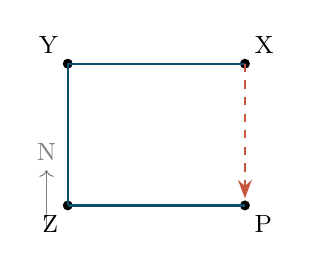
\begin{tikzpicture}[scale=0.9,every node/.style={font=\small}]
\draw[->,gray] (-0.3,-0.3)--(-0.3,0.5) node[above]{N};
\fill (0,0) circle(2pt) node[below left]{Z};
\fill (0,2) circle(2pt) node[above left]{Y};
\fill (2.5,2) circle(2pt) node[above right]{X};
\fill (2.5,0) circle(2pt) node[below right]{P};
\draw[thick,brand] (0,0)--(0,2)--(2.5,2); \draw[thick,brand] (0,0)--(2.5,0);
\draw[-Stealth,thick,accent,dashed] (2.5,2)--(2.5,0.1);
\end{tikzpicture}
\end{center}
Y is north of Z. X is east of Y. P is east of Z. Taking the standard layout, X and P are at the same east--west position, with X directly above P. So P is to the \textbf{South} of X.
\end{explain}
\end{question}

\begin{question}{47}
{Match the following four terms of Column A with that of Column B, correctly as per Pramana's reasoning.\par\smallskip\begin{tabularx}{\linewidth}{@{}>{\raggedright\arraybackslash}X>{\raggedright\arraybackslash}X@{}}\toprule
\textbf{Column A} & \textbf{Column B}\\\midrule
1. Pramana & a. The subject who knows\\
2. Pramata & b. The means of validity\\
3. Prameya & c. The resultant valid knowledge\\
4. Prama & d. The object of knowledge\\
\bottomrule\end{tabularx}\par\smallskip
The correct match is\par}
\optstwo{1-d, 2-a, 3-b, 4-c}{1-b, 2-a, 3-d, 4-c}{1-c, 2-a, 3-b, 4-d}{1-d, 2-c, 3-b, 4-a}
\answer{B}{1-b, 2-a, 3-d, 4-c}
\begin{explain}
In Nyaya epistemology:
\begin{itemize}
\item \textbf{Pramana}: the means of valid knowledge (b)
\item \textbf{Pramata}: the knower, the subject who knows (a)
\item \textbf{Prameya}: the object of knowledge (d)
\item \textbf{Prama}: the resulting valid knowledge (c)
\end{itemize}
The match is \textbf{1-b, 2-a, 3-d, 4-c}.
\end{explain}
\end{question}

\begin{question}{48}
{The ratio of the number of students studying in schools A, B and C is 6:8:7 respectively. If the number of students studying in each of the schools is increased by 20\%, 15\% and 20\% respectively, what will be the new ratio of the number of students in schools A, B and C ?\par}
\optsfour{20:19:18}{20:22:24}{21:22:23}{18:23:21}
\answer{D}{18:23:21}
\begin{explain}
New ratio $=6\times1.20 : 8\times1.15 : 7\times1.20=7.2:9.2:8.4=72:92:84=\mathbf{18:23:21}$.
\end{explain}
\end{question}

\begin{question}{49}
{The average of $1^{2}$, $2^{2}$, $3^{2}$, $4^{2}$, $5^{2}$, $6^{2}$ is\par}
\optsfour{14.69}{15.17}{16.21}{17.48}
\answer{B}{15.17}
\begin{explain}
\[\frac{1+4+9+16+25+36}{6}=\frac{91}{6}=\mathbf{15.17}\]
(Using $\sum n^2=\tfrac{n(n+1)(2n+1)}{6}=\tfrac{6\cdot7\cdot13}{6}=91$.)
\end{explain}
\end{question}

\begin{question}{50}
{The bacterial count in a certain culture (colony) increased from 1000 to 4000 in 3 days. What was the average percentage increase per day?\par}
\optsfour{49.2\%}{54.3\%}{58.7\%}{62.9\%}
\answer{C}{58.7\%}
\begin{explain}
The growth is compound (per day): $1000(1+r)^3=4000\Rightarrow(1+r)^3=4\Rightarrow1+r=\sqrt[3]4\approx1.587$.
Average daily increase $\approx\mathbf{58.7\%}$.
\end{explain}
\end{question}

\paperchapter{November 2023}{26 November 2023}{A}{50}{17th GSET}
\keytable{\kcell{1}{A} & \kcell{2}{A} & \kcell{3}{A} & \kcell{4}{B} & \kcell{5}{B} & \kcell{6}{B} & \kcell{7}{B} & \kcell{8}{C} & \kcell{9}{A} & \kcell{10}{C} \\
\kcell{11}{A} & \kcell{12}{D} & \kcell{13}{B} & \kcell{14}{B} & \kcell{15}{A} & \kcell{16}{C} & \kcell{17}{D} & \kcell{18}{B} & \kcell{19}{C} & \kcell{20}{A} \\
\kcell{21}{A} & \kcell{22}{B} & \kcell{23}{A} & \kcell{24}{D} & \kcell{25}{C} & \kcell{26}{A} & \kcell{27}{B} & \kcell{28}{A} & \kcell{29}{C} & \kcell{30}{A} \\
\kcell{31}{C} & \kcell{32}{C} & \kcell{33}{C} & \kcell{34}{C} & \kcell{35}{B} & \kcell{36}{B} & \kcell{37}{B} & \kcell{38}{D} & \kcell{39}{C} & \kcell{40}{Z} \\
\kcell{41}{A} & \kcell{42}{A} & \kcell{43}{D} & \kcell{44}{B} & \kcell{45}{C} & \kcell{46}{C} & \kcell{47}{B} & \kcell{48}{A} & \kcell{49}{C} & \kcell{50}{A}}
\begin{question}{1}
{Match X with Y.\\[2pt]
\begin{tabular}{@{}ll@{}}
\textbf{X} & \textbf{Y}\\
1. Proxemics & a. Use of touch\\
2. Kinesics & b. Use of body language\\
3. Haptics & c. Use of space\\
\end{tabular}\par}
\optsfour{1-c, 2-b, 3-a}{1-a, 2-b, 3-c}{1-b, 2-a, 3-c}{1-c, 2-a, 3-b}
\answer{A}{1-c, 2-b, 3-a}
\begin{explain}
\textbf{Proxemics} is the use of \emph{space} (c), \textbf{Kinesics} the use of \emph{body language} such as gestures, posture and facial expression (b), and \textbf{Haptics} the use of \emph{touch} (a). The match is 1-c, 2-b, 3-a.
\tip{Non-verbal codes: Kinesics (body), Proxemics (space), Haptics (touch), Chronemics (time), Paralanguage (voice qualities), Oculesics (eye contact), Artifacts (dress and objects).}
\end{explain}
\end{question}

\begin{question}{2}
{Use of 'space' in communication is called\par}
\optsfour{Proximics}{Chronomics}{Para language}{Haptics}
\answer{A}{Proximics}
\begin{explain}
The use of space and distance in communication is \textbf{Proxemics} (Edward T.~Hall). Hall described four zones: intimate (0--18 in), personal (1.5--4 ft), social (4--12 ft) and public (over 12 ft).
\why{Chronemics = use of time; Paralanguage = tone, pitch, pace and other vocal cues; Haptics = touch.}
\end{explain}
\end{question}

\begin{question}{3}
{The connotative meaning of a word is\par}
\optstwo{Subjective meaning}{Oppositive meaning}{Donotative meaning}{Real meaning}
\answer{A}{Subjective meaning}
\begin{explain}
\textbf{Connotative meaning} is the associated, emotional or \emph{subjective} meaning that a word carries beyond its dictionary sense. For example, ``home'' connotes warmth and security. \textbf{Denotative} meaning is the literal, dictionary (``real'') meaning.
\end{explain}
\end{question}

\begin{question}{4}
{In the process of communication, the receiver\par}
\optstwo{Encodes the message}{Decodes the message}{Is a channel}{Has no role}
\answer{B}{Decodes the message}
\begin{explain}
The receiver \textbf{decodes} the message, interpreting the symbols to extract meaning. The sender encodes, and the channel carries the message.
\end{explain}
\end{question}

\begin{question}{5}
{'Demophobia' refers to\par}
\optstwo{Fear of death}{Fear of crowd}{Fear of speaking}{Fear of failure}
\answer{B}{Fear of crowd}
\begin{explain}
\textbf{Demophobia} (Greek \emph{demos}, people) is the fear of crowds. It is also called enochlophobia or ochlophobia.
\why{Fear of death = thanatophobia; fear of public speaking = glossophobia; fear of failure = atychiphobia.}
\end{explain}
\end{question}

\begin{question}{6}
{Which of the following institutions responsible for quality technical and Management Higher Education in India?\par}
\optsfour{NCERT}{AICTE}{NCTE}{NIEPA}
\answer{B}{AICTE}
\begin{explain}
The \textbf{All India Council for Technical Education (AICTE)}, a statutory body under the AICTE Act 1987 (set up as an advisory body in 1945), regulates and ensures the quality of \emph{technical and management} education: engineering, pharmacy, architecture, MBA/PGDM and MCA.
\why{NCERT deals with school curriculum; NCTE with teacher education; NIEPA with educational planning and administration.}
\end{explain}
\end{question}

\begin{question}{7}
{'NAAC' assessment cycle is for\par}
\optsfour{3 years}{5 years}{10 years}{7 years}
\answer{B}{5 years}
\begin{explain}
NAAC accreditation is valid for \textbf{5 years}, after which an institution must undergo the next cycle of assessment and accreditation. (NAAC was established in 1994 by UGC and is headquartered in Bengaluru.)
\end{explain}
\end{question}

\begin{question}{8}
{The National Education Day in India is celebrated every year on\par}
\optsfour{14th November}{5th September}{11th November}{2nd October}
\answer{C}{11th November}
\begin{explain}
\textbf{National Education Day} is observed on \textbf{11 November}, the birth anniversary of \emph{Maulana Abul Kalam Azad}, India's first Education Minister (1947--58). It has been celebrated since 2008.
\why{14 November is Children's Day (Nehru), 5 September is Teachers' Day (Dr.~S.~Radhakrishnan), and 2 October is Gandhi Jayanti.}
\end{explain}
\end{question}

\begin{question}{9}
{What is the full form of ABC, according to NEP (2020) ?\par}
\optstwo{Academic Bank of Credits}{Academic Bank of Certification}{Annual Book of Credits}{Academic Basic Certification}
\answer{A}{Academic Bank of Credits}
\begin{explain}
NEP~2020 proposed an \textbf{Academic Bank of Credits (ABC)}, a digital store of the credits earned by students from recognised HEIs. It enables multiple entry and exit, credit transfer and lifelong learning. The UGC ABC Regulations were notified in 2021.
\end{explain}
\end{question}

\begin{question}{10}
{According to NIRF overall ranking 2023, which institution ranked one in India?\par}
\optstwo{IISc, Bangalore}{IISER, Pune}{IIT, Madras}{IIM, Ahmedabad}
\answer{C}{IIT, Madras}
\begin{explain}
In \textbf{NIRF 2023} (Overall category), \textbf{IIT Madras} was ranked first, as it has been every year since 2019. IISc Bengaluru was 2nd and IIT Delhi 3rd. (IISc tops the \emph{University} category.)
\end{explain}
\end{question}

\begin{question}{11}
{Which of the following diagrams correctly represents the relationship among tennis fans, cricket players and students?\par}
\optsfour{\tikz[baseline=-0.5ex,scale=0.28]{\draw (0,0.45) circle(1); \draw (-0.55,-0.45) circle(1); \draw (0.55,-0.45) circle(1);}}{\tikz[baseline=-0.5ex,scale=0.28]{\draw (0,0) circle(1); \draw (1.4,0) circle(1); \draw (2.8,0) circle(1);}}{\tikz[baseline=-0.5ex,scale=0.28]{\draw (0,0) circle(1.2); \draw (0,0) circle(0.8); \draw (0,0) circle(0.4);}}{\tikz[baseline=-0.5ex,scale=0.28]{\draw (0,0) circle(1.2); \draw (0,0) circle(0.6); \draw (2.2,0) circle(0.7);}}
\answer{A}{\tikz[baseline=-0.5ex,scale=0.28]{\draw (0,0.45) circle(1); \draw (-0.55,-0.45) circle(1); \draw (0.55,-0.45) circle(1);}}
\begin{explain}
None of the three groups is contained in another, and any two (or all three) can share members. A student may be a tennis fan, a cricket player may be a student, and a student who plays cricket may also be a tennis fan. So the diagram must show \textbf{three mutually overlapping circles} with a common central region, which is option (A).
\begin{center}
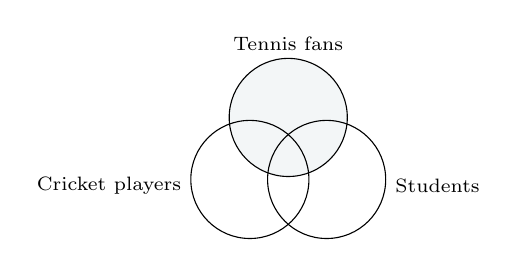
\begin{tikzpicture}[scale=0.75,font=\scriptsize]
\draw[fill=brand!10,fill opacity=0.5] (0,0.55) circle(1); \node at (0,1.8) {Tennis fans};
\draw (-0.65,-0.5) circle(1); \node[left] at (-1.65,-0.6) {Cricket players};
\draw (0.65,-0.5) circle(1); \node[right] at (1.65,-0.6) {Students};
\end{tikzpicture}
\end{center}
\end{explain}
\end{question}

\begin{question}{12}
{'Umpire' is related to 'Match' in the same way as 'Judge' is related to\par}
\optsfour{Court}{Lawyer}{Judgement}{Law suit}
\answer{D}{Law suit}
\begin{explain}
An \textbf{umpire} presides over and gives decisions in a \textbf{match}; likewise, a \textbf{judge} presides over and decides a \textbf{law suit} (case). The relation is \emph{adjudicator : the event being adjudicated}.
\why{A court is the \emph{place} (the analogue of the stadium), a lawyer is a participant, and a judgement is the decision itself (the analogue of the umpire's ruling).}
\end{explain}
\end{question}

\begin{question}{13}
{In question below is given a statement followed by assumptions numbered I and II. Consider the statement and decide which of the given assumption is implicit ?\newline Statement: If you want to give any advertisement give it in newspaper "X" - A tells to B.\newline Assumptions: \newline I. 'B' wants to publicise his products.\newline II. Newspaper 'X' has a wide circulation.\par}
\optstwo{Only assumption I is implicit}{Only assumption II is implicit}{Either I or II is implicit}{Neither I nor II is implicit}
\answer{B}{Only assumption II is implicit}
\begin{explain}
A advises B to advertise in newspaper X. This advice assumes that X reaches many people, i.e.\ that it has a wide circulation, so assumption II is implicit. The statement is conditional (``\emph{If} you want to give any advertisement \ldots''), so it does not assume that B actually wants to publicise products. Assumption I is not implicit.
\textbf{Only II is implicit.}
\end{explain}
\end{question}

\begin{question}{14}
{P, Q, R, S and U are the family members. P and Q are real brothers. R is a sister of P. S is a father of P. U is a father of S. What is the relation between P and U?\par}
\optstwo{Granddaughter and grandfather}{Grandson and grandfather}{Father and son}{Father and daughter}
\answer{B}{Grandson and grandfather}
\begin{explain}
S is P's father and U is S's father, so U is P's paternal \textbf{grandfather}. P is a ``real brother'' of Q, so P is male, a \textbf{grandson}.
\begin{center}
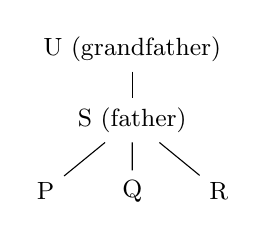
\begin{tikzpicture}[font=\small,level distance=9mm,sibling distance=11mm]
\node{U (grandfather)} child{node{S (father)} child{node{P}} child{node{Q}} child{node{R}}};
\end{tikzpicture}
\end{center}
\end{explain}
\end{question}

\begin{question}{15}
{Find the next term of given series.\newline A7T, E12Q, I19L, \blank{}\par}
\optsfour{M28E}{M25E}{M24C}{M29E}
\answer{A}{M28E}
\begin{explain}
Three independent patterns:
\begin{itemize}
\item First letters: A, E, I, \textbf{M} (+4 each).
\item Numbers: 7, 12, 19, \textbf{28} (+5, +7, +9).
\item Last letters: T, Q, L, \textbf{E} ($-3$, $-5$, $-7$: T(20)$\rightarrow$Q(17)$\rightarrow$L(12)$\rightarrow$E(5)).
\end{itemize}
The next term is \textbf{M28E}.
\end{explain}
\end{question}

\begin{question}{16}
{Which of the following are a web browser?\newline 1. Microsoft edge\newline 2. Google chrome\newline 3. Mozilla firefox\newline 4. Opera\newline 5. Safari\par}
\optstwo{1, 2, 3 and 4}{1, 2, 4 and 5}{1, 2, 3, 4 and 5}{1, 2, 3 and 5}
\answer{C}{1, 2, 3, 4 and 5}
\begin{explain}
All five are web browsers: Microsoft Edge, Google Chrome, Mozilla Firefox, Opera and Apple Safari. The answer is 1, 2, 3, 4 and 5.
\end{explain}
\end{question}

\begin{question}{17}
{Which of the following are used in video-conferencing ?\newline 1. Google Meet\newline 2. Microsoft Team\newline 3. Cisco WebEx\newline 4. Skype\newline 5. Zoom meeting\par}
\optstwo{1, 2, 3 and 5}{1, 2, 4 and 5}{1, 3, 4 and 5}{1, 2, 3, 4 and 5}
\answer{D}{1, 2, 3, 4 and 5}
\begin{explain}
All five are video-conferencing tools: Google Meet, Microsoft Teams, Cisco WebEx, Skype and Zoom. The answer is (D).
\end{explain}
\end{question}

\begin{question}{18}
{The first page of website is called\par}
\optsfour{Main page}{Home page}{Front page}{Open page}
\answer{B}{Home page}
\begin{explain}
The first (main entry) page of a website is its \textbf{home page}, usually reached at the site's root URL (e.g.\ \texttt{www.example.com/}). It links to all other sections of the site.
\end{explain}
\end{question}

\begin{question}{19}
{Given below are two statements:\newline Statement I: SWAYAM stands for study webs of active learning for young aspiring minds.\newline Statement II: All MOOCs on the SWAYAM portal are credit-based MOOCs.\newline In light of the above statements, choose the correct answer from the options given below:\par}
\optsone{Both Statement I and Statement II are true}{Both Statement I and Statement II are false}{Statement I is true but Statement II is false}{Statement I is false but Statement II is true}
\answer{C}{Statement I is true but Statement II is false}
\begin{explain}
\textbf{Statement I} is true: SWAYAM stands for \emph{Study Webs of Active-Learning for Young Aspiring Minds}.
\textbf{Statement II} is false: not all SWAYAM courses are credit-based. Many are non-credit or certificate courses. Credit transfer (up to 40\% of a programme's credits under the UGC SWAYAM Regulations, 2021) applies only to courses so designated and accepted by the parent university.
\end{explain}
\end{question}

\begin{question}{20}
{Given below are two statements, one is labeled as Assertion A and the other is labeled as Reason R.\newline Assertion (A): 'Router' is considered as both input and output device.\newline Reason (R): 'Router' can send data and receive data at the same time.\newline In light of the above statements, choose the correct answer from the options given below:\par}
\optsone{Both (A) and (R) are true and (R) is the correct explanation of (A)}{Both (A) and (R) are true but (R) is not the correct explanation of (A)}{(A) is true but (R) is false}{(A) is false but (R) is true}
\answer{A}{Both (A) and (R) are true and (R) is the correct explanation of (A)}
\begin{explain}
The official key accepts both statements, with R explaining A. A router both \emph{receives} data packets (from a network or modem) and \emph{sends} (forwards) them to other devices, so it performs input and output functions at the same time. Its two-way data transfer is the reason it is treated as both an input and an output device.
\tip{Strictly, a router is a \emph{networking} device. In exam questions, devices that both send and receive data (modem, router, touch screen) are usually accepted as ``input--output'' devices.}
\end{explain}
\end{question}

\begin{question}{21}
{Teaching at higher education should avoid the approach of\par}
\optsone{Covering every bit of content step by step in the class}{Guided learning and self learning}{Motivating learner, use of self learning and lectures on difficult content}{Combination of self learning with digital platform based teaching}
\answer{A}{Covering every bit of content step by step in the class}
\begin{explain}
Higher education aims at developing independent, critical and self-directed learners. \textbf{Covering every bit of content step by step in class} (spoon-feeding) should be avoided. Guided learning, self-learning, motivation, lectures on difficult content and blended digital learning are all desirable.
\end{explain}
\end{question}

\begin{question}{22}
{In Discussion method of teaching which type of questions have limited role ?\par}
\optstwo{Higher order questions}{Yes-no type of questions}{Hypothetical issue related questions}{Critical awareness related questions}
\answer{B}{Yes-no type of questions}
\begin{explain}
A discussion thrives on open-ended, thought-provoking questions. \textbf{Yes/no (closed) questions} have a limited role because they end the exchange with a one-word answer and do not stimulate reasoning or debate.
\end{explain}
\end{question}

\begin{question}{23}
{Which of the following set belongs to teaching?\par}
\optsone{Instruction, scientific inquiry, case study, brainstorming}{Preaching, case study, brainstorming and indoctrination}{Brainstorming, preaching, surmons, instruction}{Tutorial, case study, brainstorming, indoctrination}
\answer{A}{Instruction, scientific inquiry, case study, brainstorming}
\begin{explain}
\textbf{Teaching} involves rational, democratic activities that respect the learner's reasoning: instruction, scientific inquiry, case study and brainstorming. \textbf{Indoctrination} and \textbf{preaching} (sermons) try to implant beliefs without inviting reasoning, so they are not teaching in the true sense.
\why{Options (B), (C) and (D) each contain preaching, sermons or indoctrination.}
\end{explain}
\end{question}

\begin{question}{24}
{Which of the following set of variables of learner largely influence the learning outcomes?\par}
\optsone{Motivation, comprehension, gender, cognition}{Study habit, religion, motivation, socio-economic status}{Religion, socio-economic status, vocabulary, cognition}{Cognition, study habit, comprehension, motivation}
\answer{D}{Cognition, study habit, comprehension, motivation}
\begin{explain}
The learner variables that largely determine learning outcomes are psychological and academic: \textbf{cognition} (intellectual ability), \textbf{study habits}, \textbf{comprehension} and \textbf{motivation}.
\why{Gender and religion are not determinants of learning outcomes, so any set containing them is wrong.}
\end{explain}
\end{question}

\begin{question}{25}
{Characteristics of teaching as profession does not ensure\par}
\optsone{Having a code of conduct}{Freedom to work independently}{Good earning and family life}{Freedom of research and student counselling}
\answer{C}{Good earning and family life}
\begin{explain}
Teaching as a profession is characterised by a \textbf{code of conduct (ethics)}, \textbf{professional autonomy} (freedom to work independently) and \textbf{academic freedom} in research and counselling. A \textbf{good income and family life} is a personal benefit, not a defining characteristic that the profession ensures.
\end{explain}
\end{question}

\begin{question}{26}
{Which of the following are Sustainable Development Goals (SDGs)?\newline 1. Clean water and sanitation\newline 2. Deforestation\newline 3. Climate action\newline 4. Quality education\newline 5. Affordable and clean energy\newline Choose the correct answer from the options given below :\par}
\optsfour{1, 3, 4 and 5}{1, 3 and 5}{1, 2, 3 and 5}{1, 3 and 4}
\answer{A}{1, 3, 4 and 5}
\begin{explain}
SDG~6 (Clean water \& sanitation), SDG~13 (Climate action), SDG~4 (Quality education) and SDG~7 (Affordable \& clean energy) are all goals. \textbf{Deforestation} is a \emph{problem}, not a goal (forests fall under SDG~15, \emph{Life on land}). The answer is 1, 3, 4 and 5.
\end{explain}
\end{question}

\begin{question}{27}
{Match the following and choose the correct option given below:\\[2pt]
\begin{tabular}{@{}ll@{}}
\textbf{G20 Presidency year} & \textbf{Nation}\\
I. 2022 & a. Brazil\\
II. 2023 & b. India\\
III. 2024 & c. South Africa\\
IV. 2025 & d. Indonesia\\
\end{tabular}\par}
\optstwo{I-d, II-b, III-c, IV-a}{I-d, II-b, III-a, IV-c}{I-a, II-b, III-c, IV-d}{I-b, II-c, III-d, IV-a}
\answer{B}{I-d, II-b, III-a, IV-c}
\begin{explain}
G20 presidencies: \textbf{2022 Indonesia} (Bali Summit), \textbf{2023 India} (New Delhi Summit; theme \emph{Vasudhaiva Kutumbakam: One Earth, One Family, One Future}), \textbf{2024 Brazil} (Rio de Janeiro), \textbf{2025 South Africa} (Johannesburg). The match is I-d, II-b, III-a, IV-c.
\end{explain}
\end{question}

\begin{question}{28}
{Recently in February 2023, a large lithium mineral reserve was found in which State ?\par}
\optstwo{Jammu and Kashmir}{Gujarat}{Jharkhand}{Bihar}
\answer{A}{Jammu and Kashmir}
\begin{explain}
In February 2023 the Geological Survey of India announced inferred lithium resources of about \textbf{5.9 million tonnes} in the \textbf{Salal-Haimana area of Reasi district, Jammu \& Kashmir}, India's first major lithium find. Lithium is vital for EV batteries.
\end{explain}
\end{question}

\begin{question}{29}
{Which of the following cyclone has affected the east coast of India in last few years?\newline 1. Cyclone Biparjoy\newline 2. Cyclone Fani\newline 3. Cyclone Taukte\newline 4. Cyclone Amphan\newline Choose the correct answer from the options given below :\par}
\optsfour{1, 2 and 3}{1 and 3}{2 and 4}{1, 3 and 4}
\answer{C}{2 and 4}
\begin{explain}
East-coast (Bay of Bengal) cyclones: \textbf{Fani} (May 2019, Odisha) and \textbf{Amphan} (May 2020, West Bengal).
Biparjoy (2023) and Tauktae (2021) struck the \emph{west} coast (Gujarat). The answer is 2 and 4.
\end{explain}
\end{question}

\begin{question}{30}
{Given below are two statements, one is labeled as Assertion (A) and the other is labeled as Reason (R).\newline Assertion (A): Air Quality Index (AQI) of City-X is 257, while that of City-Y is 65 in the month of August - 2023.\newline Reason (R): City-X is more air polluted than City-Y.\newline In light of the above statements, choose the correct answer from the options given below:\par}
\optsone{Both (A) and (R) are true and (R) is the correct explanation of (A)}{Both (A) and (R) are true but (R) is not the correct explanation of (A)}{(A) is true but (R) is false}{(A) is false but (R) is true}
\answer{A}{Both (A) and (R) are true and (R) is the correct explanation of (A)}
\begin{explain}
An AQI of 257 falls in the \emph{Poor} band (201--300), while an AQI of 65 is \emph{Satisfactory} (51--100). A higher AQI means more air pollution, so City-X is more polluted, and this is exactly what explains the AQI values. Both are true and R explains A.
\end{explain}
\end{question}

\begin{question}{31}
{Scientific method of research involves the process of\par}
\optstwo{Induction}{Deduction}{Indo-deductive method}{Contemplation}
\answer{C}{Indo-deductive method}
\begin{explain}
The scientific method combines \textbf{induction} (observations $\rightarrow$ generalisation or hypothesis) and \textbf{deduction} (hypothesis $\rightarrow$ testable predictions $\rightarrow$ verification). This cycle is called the \textbf{inductive--deductive} method (the ``indo-deductive'' of the option). It is associated with Charles Darwin and John Dewey's reflective thinking.
\end{explain}
\end{question}

\begin{question}{32}
{Snowball sampling method\par}
\optsone{Is most preferred technique during survey method}{Provides representative sample for experimental study}{Is suitable to identify sample from unknown population}{Use rolling ball machine to get random sample}
\answer{C}{Is suitable to identify sample from unknown population}
\begin{explain}
In \textbf{snowball sampling} each respondent refers further respondents, so the sample ``snowballs''. It suits \textbf{hidden, rare or unknown populations} (drug users, migrant workers, rare-disease patients) for which no sampling frame exists.
\why{It is non-probability, so it does not give a representative sample, and it has nothing to do with a rolling-ball machine.}
\end{explain}
\end{question}

\begin{question}{33}
{Which of the following is the correct statement of historical research?\par}
\optsone{It is not a scientific inquiry}{The extrinsic data validation is assumptive}{The findings are subjective to a great extent}{Reveals past with no contribution to future}
\answer{C}{The findings are subjective to a great extent}
\begin{explain}
Historical research reconstructs the past from documents and relics, and the researcher's interpretation plays a large role. Its findings are therefore \textbf{subjective to a great extent}.
\why{It \emph{is} a scientific inquiry. Sources are validated through external criticism (authenticity) and internal criticism (credibility), so validation is not ``assumptive''. It helps us understand the present and plan for the future.}
\end{explain}
\end{question}

\begin{question}{34}
{Which of the following is a discrete variable?\par}
\optstwo{Human IQ score}{Human height}{Number of human beings}{Human weight}
\answer{C}{Number of human beings}
\begin{explain}
A \textbf{discrete variable} takes only separate, countable values (0, 1, 2, \ldots). The \textbf{number of human beings} is counted in whole numbers, so it is discrete.
\why{Height and weight are continuous (they can take any value in a range). IQ is treated as a continuous measure on an interval scale.}
\end{explain}
\end{question}

\begin{question}{35}
{Which of the following statement is true for Swayamprabha ?\par}
\optsone{They are MOOCs and certified for credit consideration by universities}{They are educational programmes under direct-to-home}{One has to pay to subscribe the programme}{They are focussed to the course content from 1st standard to 12th standard}
\answer{B}{They are educational programmes under direct-to-home}
\begin{explain}
SWAYAM Prabha is a group of 40 \textbf{DTH (Direct-to-Home)} educational TV channels telecasting 24$\times$7 via the GSAT-15 satellite. They are \textbf{free}, cover school, higher and lifelong education, and are not credit-bearing MOOCs.
\end{explain}
\end{question}

\begin{question}{36}
{Ravi travelled 4 km straight towards South. He turned left and travelled 6 km straight, then turned right and travelled 4 km straight. How far is he from the starting point ?\par}
\optsfour{8 km}{10 km}{12 km}{15 km}
\answer{B}{10 km}
\begin{explain}
\begin{center}
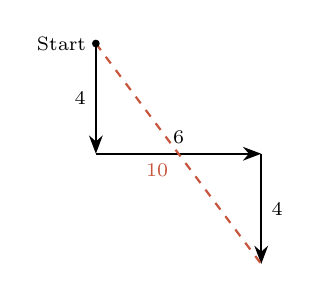
\begin{tikzpicture}[scale=0.35,font=\scriptsize,>=Stealth]
\draw[thick,->] (0,0) -- node[left]{4} (0,-4);
\draw[thick,->] (0,-4) -- node[above]{6} (6,-4);
\draw[thick,->] (6,-4) -- node[right]{4} (6,-8);
\draw[dashed,accent,thick] (0,0) -- node[below left]{10} (6,-8);
\fill (0,0) circle(4pt) node[left]{Start};
\end{tikzpicture}
\end{center}
South 4 km, left (east) 6 km, right (south) 4 km. Net: 8 km south and 6 km east.
\[\text{Distance}=\sqrt{8^2+6^2}=\sqrt{100}=\mathbf{10\ km}\]
\end{explain}
\end{question}

\begin{question}{37}
{The following diagram shows the number of students who got distinction in the subject out of 500 students.\par}
\qfigure{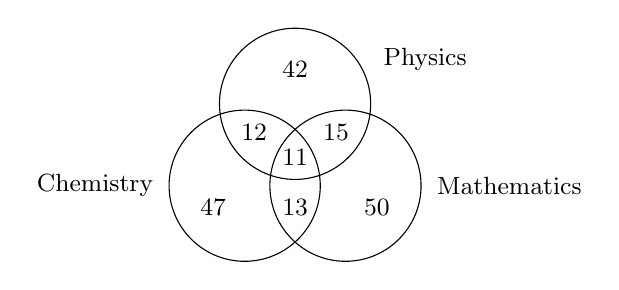
\begin{tikzpicture}[scale=0.8,font=\small]
\draw (0,0.9) circle(1.2); \draw (-0.8,-0.4) circle(1.2); \draw (0.8,-0.4) circle(1.2);
\node at (0,1.45) {42}; \node at (-1.3,-0.75) {47}; \node at (1.3,-0.75) {50};
\node at (-0.65,0.45) {12}; \node at (0.65,0.45) {15}; \node at (0,-0.75) {13}; \node at (0,0.05) {11};
\node[right] at (1.25,1.6) {Physics}; \node[left] at (-2.1,-0.4) {Chemistry}; \node[right] at (2.1,-0.4) {Mathematics};
\end{tikzpicture}}
What is the percentage of students who got distinction only in two subjects?
\optsfour{6\%}{8\%}{10\%}{12\%}
\answer{B}{8\%}
\begin{explain}
``Only two subjects'' means the pairwise overlaps, excluding the centre (11):
\[12\ (\text{P}\cap\text{C})+15\ (\text{P}\cap\text{M})+13\ (\text{C}\cap\text{M})=40\qquad\frac{40}{500}\times100=\mathbf{8\%}\]
\end{explain}
\end{question}

\begin{question}{38}
{A car travels 25 km at a speed of 25 kmh, next 25 km at a speed of 50 kmh and the next 25 km at a speed of 75 kmh. What is the average speed of the car?\par}
\optsfour{64 kmh}{50 kmh}{46 kmh}{41 kmh}
\answer{D}{41 kmh}
\begin{explain}
When equal \emph{distances} are covered at different speeds, find the total time:
\[t=\frac{25}{25}+\frac{25}{50}+\frac{25}{75}=1+\frac12+\frac13=\frac{11}{6}\text{ h}\qquad \bar v=\frac{75}{11/6}=\frac{450}{11}\approx\mathbf{41\ km/h}\]
(This is the harmonic mean of 25, 50 and 75.)
\end{explain}
\end{question}

\begin{question}{39}
{The quarterly sales of a particular mobile in rural and urban areas during year 2022 is as follows:\par}
\qfigure{\begin{tabular}{lcccc}\toprule
\textbf{Area} & \multicolumn{4}{c}{\textbf{Sales in 100 units}}\\\cmidrule(l){2-5}
& Q$_1$ & Q$_2$ & Q$_3$ & Q$_4$\\\midrule
Rural & 30 & 25 & 40 & 35\\ Urban & 40 & 60 & 40 & 70\\\bottomrule
\end{tabular}}
What is the percentage of sales during Q$_3$?
\optsfour{20.5\%}{25.0\%}{23.5\%}{30.9\%}
\answer{C}{23.5\%}
\begin{explain}
Total sales $=(30+25+40+35)+(40+60+40+70)=130+210=340$.\\
Q$_3$ sales $=40+40=80$.
\[\frac{80}{340}\times100=\mathbf{23.5\%}\]
\end{explain}
\end{question}

\begin{question}{40}
{Given the following data:
\begin{center}
\begin{tabular}{ccccc}
22 & 26 & 18 & 15 & 30\\ 20 & 16 & 22 & 24 & 25\\ 38 & 36 & 28 & 26 & 25\\ 40 & 34 & 36 & 20 & 22\\
\end{tabular}
\end{center}
What is the percentage of observation below average?\par}
\optsfour{40\%}{45\%}{50\%}{60\%}
\dropped{}
\begin{explain}
Sum of the 20 observations $=111+107+153+152=523$, so the mean $=523/20=26.15$.
Values below 26.15: 22, 26, 18, 15 (row 1); 20, 16, 22, 24, 25 (row 2); 26, 25 (row 3); 20, 22 (row 4), which is 13 values.
\[\frac{13}{20}\times100=65\%\]
65\% is not among the options, which is why the agency \textbf{dropped} the question.
\end{explain}
\end{question}

\begin{context}
\textbf{Directions for Q.~41 to 45:} Read the following paragraph and answer the questions given below it.\par\smallskip
You have studied that elemental oxygen is found in the atmosphere in the form of a diatomic molecule (O$_2$). However, in the upper part of the atmosphere, oxygen is present in its triatomic form called ozone (O$_3$). Ozone forms a layer at a height of 15--60 km in the stratosphere. The ozone levels are low over or near the equator and high near the poles.

Ozone is a highly reactive form of molecular oxygen and is poisonous for us. But we are protected from its harmful effects as it is unstable near the surface of the earth. Further, ozone protects the biosphere from the harmful ultraviolet radiations. It filters out the radiations coming to the earth and maintains the temperature of the earth.

Over the last few years, it has been observed that ozone layer is thinning out because of the excessive use of chlorofluorocarbons (CFCs) by human beings. Once considered as miracle compounds, CFCs were being used as propellants in aerosols and as coolants for refrigerators and air conditioners. But now, they are considered harmful compounds as they are stable, do not degrade by any biological process and harm the protective O$_3$ layer by reacting with O$_3$ molecules.
\end{context}
\begin{question}{41}
{The ozone levels is low at\par}
\optstwo{Equator}{Poles}{Both equator and poles}{Neither equator nor poles}
\answer{A}{Equator}
\begin{explain}
``The ozone levels are \textbf{low over or near the equator} and high near the poles.''
\end{explain}
\end{question}

\begin{question}{42}
{Ozone means\par}
\optstwo{A triatomic form of oxygen}{Diatomic molecular}{Elementary oxygen}{Carbon dioxide (CO2)}
\answer{A}{A triatomic form of oxygen}
\begin{explain}
``\ldots oxygen is present in its \textbf{triatomic form} called ozone (O$_3$).''
\end{explain}
\end{question}

\begin{question}{43}
{Ozone is a molecular oxygen which is\par}
\optstwo{Neutral}{Inactive}{Non-poisonous}{Highly reactive}
\answer{D}{Highly reactive}
\begin{explain}
``Ozone is a \textbf{highly reactive} form of molecular oxygen and is poisonous for us.''
\end{explain}
\end{question}

\begin{question}{44}
{Ozone protects biosphere from\par}
\optstwo{Clouds and acid rains}{Ultraviolet radiations}{Pollution}{Cyclone}
\answer{B}{Ultraviolet radiations}
\begin{explain}
``\ldots ozone protects the biosphere from the harmful \textbf{ultraviolet radiations}.''
\end{explain}
\end{question}

\begin{question}{45}
{The reason for thinning of ozone level\par}
\optstwo{Excess use of O2}{Release of CO2}{Excessive use of chlorofluorocarbons}{Excess release of carbon monoxide}
\answer{C}{Excessive use of chlorofluorocarbons}
\begin{explain}
``\ldots ozone layer is thinning out because of the \textbf{excessive use of chlorofluorocarbons (CFCs)}.''
\tip{The Montreal Protocol (1987) phases out ozone-depleting substances; 16 September is International Day for the Preservation of the Ozone Layer.}
\end{explain}
\end{question}

\begin{question}{46}
{A mixture contains sugar solution and colored water in the ratio 4: 3. If 10 litres of colored water is added to the mixture, the ratio becomes 4: 5. What is the initial quantity of sugar solution in the given mixture ?\par}
\optsfour{8 litres}{10 litres}{20 litres}{25 litres}
\answer{C}{20 litres}
\begin{explain}
Let sugar solution $=4x$ and coloured water $=3x$.
\[\frac{4x}{3x+10}=\frac45\Rightarrow20x=12x+40\Rightarrow x=5\]
Initial sugar solution $=4x=\mathbf{20}$ litres.
\end{explain}
\end{question}

\begin{question}{47}
{Three friends P, Q and R started a business, each investing Rs. 10,000. After 5 months, P withdrews Rs. 3,000, Q withdrews Rs. 2,000 and R invested Rs. 3,000 more. At the end of the year a total profit of Rs. 34,600 was recorded. What is the share of P, Q and R respectively?\par}
\optstwo{10,600, 9,900, 14,100}{9,900, 10,600, 14,100}{14,100, 10,600, 9,900}{10,600, 14,100, 9,900}
\answer{B}{9,900, 10,600, 14,100}
\begin{explain}
Profit is shared in the ratio of capital $\times$ time (month-units):
\begin{center}\small
\begin{tabular}{lll}\toprule
Partner & Investment $\times$ months & Total\\\midrule
P & $10{,}000\times5+7{,}000\times7$ & 99{,}000\\
Q & $10{,}000\times5+8{,}000\times7$ & 1{,}06{,}000\\
R & $10{,}000\times5+13{,}000\times7$ & 1{,}41{,}000\\\bottomrule
\end{tabular}
\end{center}
Ratio $=99:106:141$ (sum 346). Shares of Rs.~34{,}600: P $=9{,}900$, Q $=10{,}600$, R $=14{,}100$.
\end{explain}
\end{question}

\begin{question}{48}
{Five ships J, K, L, M and N are to be unloaded on 5 consecutive days beginning from Monday to Friday.\newline I. Each ship takes exactly one day to unload.\newline II. K must be unloaded on the day preceding the day on which M and N are unloaded.\newline III. L cannot be unloaded on Tuesday.\newline IV. M is the second ship to be unloaded after J is unloaded.\newline If M is unloaded on Friday, which one of the following is true?\par}
\optstwo{J is unloaded on Wednesday}{K is unloaded on Tuesday}{L is unloaded on Monday}{N is unloaded on Thursday}
\answer{A}{J is unloaded on Wednesday}
\begin{explain}
M is on Friday. M is the second ship after J, so J is on \textbf{Wednesday}. K must come before both M and N, and L cannot be on Tuesday. The remaining days (Mon, Tue, Thu) take K, L, N with K before N, e.g.\ K--Mon, N--Tue, L--Thu. Among the options, only ``J is unloaded on Wednesday'' is necessarily true.
\begin{center}\small
\begin{tabular}{ccccc}\toprule Mon & Tue & Wed & Thu & Fri\\\midrule K & N & \textbf{J} & L & \textbf{M}\\\bottomrule\end{tabular}
\end{center}
\end{explain}
\end{question}

\begin{question}{49}
{If $+$ means $\times$, $-$ means $+$, $\times$ means $\div$ and $\div$ means $-$, then the value of $6-9+8\times3\div20$ is\par}
\optsfour{-2}{6}{10}{12}
\answer{C}{10}
\begin{explain}
Substitute the symbols: $6-9+8\times3\div20$ becomes
\[6+9\times8\div3-20=6+\frac{72}{3}-20=6+24-20=\mathbf{10}\]
\end{explain}
\end{question}

\begin{question}{50}
{Three positions of the same dice are given below. Which number will come in place of x?\par}
\qfigure{\die{1}{6}{3}\qquad\die{3}{5}{4}\qquad\die{4}{2}{x}}
\optsfour{1}{3}{5}{6}
\answer{A}{1}
\begin{explain}
Die (i): top 1, front 6, right 3. Die (ii): top 3, front 5, right 4. Die (iii): top 4, front 2, right x.
\begin{enumerate}
\item Faces adjacent to 3 are 1, 6 (die i) and 5, 4 (die ii), so \textbf{3 is opposite 2}.
\item Turning die (i) so that 3 comes on top and matching die (ii) gives the opposite pairs \textbf{1--5}, \textbf{6--4}, \textbf{3--2}.
\item In die (iii), 4 is on top (so 6 is at the bottom) and 2 is in front (so 3 is at the back). The two side faces are 1 and 5. Using the orientation fixed by die (i) (with 4 behind and 2 on the left when 1 is on top and 6 in front), bringing 4 to the top and 2 to the front puts \textbf{1 on the right}.
\end{enumerate}
Hence x $=$ \textbf{1}.
\end{explain}
\end{question}

\paperchapter{November 2022}{6 November 2022}{A}{50}{16th GSET}
\keytable{\kcell{1}{C} & \kcell{2}{C} & \kcell{3}{D} & \kcell{4}{C} & \kcell{5}{C} & \kcell{6}{B} & \kcell{7}{D} & \kcell{8}{A} & \kcell{9}{B} & \kcell{10}{C} \\
\kcell{11}{D} & \kcell{12}{B} & \kcell{13}{B} & \kcell{14}{C} & \kcell{15}{A} & \kcell{16}{A} & \kcell{17}{D} & \kcell{18}{C} & \kcell{19}{B} & \kcell{20}{C} \\
\kcell{21}{Z} & \kcell{22}{D} & \kcell{23}{A} & \kcell{24}{C} & \kcell{25}{A} & \kcell{26}{B} & \kcell{27}{C} & \kcell{28}{A} & \kcell{29}{A} & \kcell{30}{D} \\
\kcell{31}{B} & \kcell{32}{A} & \kcell{33}{B} & \kcell{34}{D} & \kcell{35}{B} & \kcell{36}{D} & \kcell{37}{B} & \kcell{38}{B} & \kcell{39}{D} & \kcell{40}{B} \\
\kcell{41}{A} & \kcell{42}{D} & \kcell{43}{B} & \kcell{44}{D} & \kcell{45}{C} & \kcell{46}{D} & \kcell{47}{C} & \kcell{48}{C} & \kcell{49}{D} & \kcell{50}{D}}
\begin{context}
\textbf{Directions for Q.~1 to 5:} Read the following passage and answer the questions.\par\smallskip
At first sight silence would seem to be the essence of non communication. Yet we know that in some circumstances silence can speak volumes. It is also a potent tool in the communication tool box, for the speaker, as it adds emphasis to point, allowing time for its full significance to sink in. Handled skillfully, it can build up anticipation for what is to come the pregnant pause. It gives opportunity to make eye contact with audience and gauge their reactions. It is an essential component of the timing of one's delivery. For the listener silence can buy time, either to digest what has been said or to consider a response, or both. Silence will, often lure the speaker into saying more than he or she may have intended.
\end{context}
\begin{question}{1}
{Silence is an essential component of\par}
\optstwo{Non-communication}{Gauging reaction of people}{The timing of one's delivery}{Distraction}
\answer{C}{The timing of one's delivery}
\begin{explain}
The passage states directly: ``It is an essential component of \textbf{the timing of one's delivery}.''
\why{``Non-communication'' is what silence \emph{seems} to be at first sight, a view the passage then rejects. Gauging reactions is an \emph{opportunity} that silence gives. Distraction is not mentioned.}
\end{explain}
\end{question}

\begin{question}{2}
{According to the author, the pregnant pause\par}
\optstwo{Breaks up communication}{Helps communication}{Build up anticipation}{Leads to confusion}
\answer{C}{Build up anticipation}
\begin{explain}
``Handled skillfully, it can \textbf{build up anticipation} for what is to come: the pregnant pause.'' A pregnant pause is a deliberate silence full of meaning that makes the audience wait for what follows.
\end{explain}
\end{question}

\begin{question}{3}
{For the listener silence can\par}
\optstwo{Emphasize a point}{Be a potent tool}{Speak volumes}{Buy time}
\answer{D}{Buy time}
\begin{explain}
``For the listener silence can \textbf{buy time}, either to digest what has been said or to consider a response.''
\why{Emphasising a point, being a potent tool and speaking volumes are described as uses of silence for the \emph{speaker} or in general.}
\end{explain}
\end{question}

\begin{question}{4}
{Silence seems to be essence of\par}
\optstwo{Communication}{Transmission}{Non-Communication}{Communication tool box}
\answer{C}{Non-Communication}
\begin{explain}
``At first sight silence would seem to be the essence of \textbf{non communication}.''
\end{explain}
\end{question}

\begin{question}{5}
{What provides an opportunity to make eye contact with the audience ?\par}
\optsfour{Communication}{Discussion}{Silence}{Gesture}
\answer{C}{Silence}
\begin{explain}
``It [silence] gives opportunity to make \textbf{eye contact} with audience and gauge their reactions.''
\end{explain}
\end{question}

\begin{question}{6}
{Which of the following are considered as both input and output devices ?\newline a. Touch screen\newline b. USB memory devices\newline c. CD drive\newline d. Screen projector\par}
\optsfour{a, c and d}{a, b and c}{a, b and d}{b, c and d}
\answer{B}{a, b and c}
\begin{explain}
Devices that both \emph{accept} and \emph{deliver} data are input/output devices:
\begin{itemize}
\item \textbf{Touch screen}: displays output and takes touch input.
\item \textbf{USB memory (pen drive)}: data can be written to it and read from it.
\item \textbf{CD drive} (read/write): reads from and writes to discs.
\end{itemize}
A \textbf{screen projector} only displays output. Hence a, b and c.
\end{explain}
\end{question}

\begin{question}{7}
{Which of the following statements are true ?\newline a. Cache memory is used to enhance the performance of computer system.\newline b. Primary memory is also known as main memory.\newline c. Hard disk is an example of secondary memory.\newline d. Static Random Access Memory (SRAM) is not a Cache memory.\par}
\optsone{a and b are true, while c and d are false}{a and c are true, while b and d are false}{b, c and d are true, while a is false}{a, b and c are true, while d is false}
\answer{D}{a, b and c are true, while d is false}
\begin{explain}
(a) True: cache is a small, very fast memory between the CPU and RAM that speeds up processing.
(b) True: primary memory (RAM/ROM) is also called main memory.
(c) True: the hard disk is secondary (auxiliary) storage.
(d) False: \textbf{SRAM is precisely the memory used for cache}, because it is fast and needs no refreshing. DRAM is used for main memory.
Hence a, b and c are true and d is false.
\end{explain}
\end{question}

\begin{question}{8}
{Which of the following are characteristics of CC-BY SA?\newline a. Allows to copy and publish\newline b. Attribution required\newline c. Cannot be used commercially\newline d. Cannot be modified and adapted\newline e. Cannot change license\par}
\optsfour{a, b and e}{a, b, d and e}{a, c, d and e}{b, d and e}
\answer{A}{a, b and e}
\begin{explain}
\textbf{CC BY-SA} (Creative Commons \emph{Attribution--ShareAlike}):
\begin{itemize}
\item allows copying, redistribution and publishing (a);
\item requires \textbf{attribution} to the creator (b);
\item permits commercial use, so (c) is wrong;
\item permits modification and adaptation, so (d) is wrong;
\item derivatives must be released \textbf{under the same licence}, so the licence cannot be changed (e).
\end{itemize}
The answer is a, b and e.
\tip{CC elements: BY = attribution, SA = share-alike, NC = non-commercial, ND = no derivatives. CC0 = public-domain dedication.}
\end{explain}
\end{question}

\begin{question}{9}
{In relation to NMEICT mission document, which of the following is not true for opportunities of ICT in education?\par}
\optsone{Availability of EduSAT}{High power consumption connectivity and computing devices}{The abundance of knowledge on the internet}{Rapidly expanding network of cyber kiosks and cyber cafes}
\answer{B}{High power consumption connectivity and computing devices}
\begin{explain}
The \emph{National Mission on Education through ICT (NMEICT)} lists as opportunities the availability of EduSAT, the abundance of knowledge on the internet, and the fast-growing network of cyber kiosks and cafes. The mission document looks for \textbf{low}-power, low-cost connectivity and devices (e.g.\ the low-cost \emph{Aakash} tablet), so ``high power consumption'' is \emph{not} an opportunity.
\end{explain}
\end{question}

\begin{question}{10}
{Which of the following has been conceived as 'One Stop Education Portal'?\par}
\optsfour{SAMAGRA}{SAMARTH}{SAKSHAT}{DIKSHA}
\answer{C}{SAKSHAT}
\begin{explain}
\textbf{SAKSHAT}, launched on 30 October 2006 by MHRD, was conceived as a \textbf{``One Stop Education Portal''} addressing the educational needs of learners from school to postgraduate level. It is the portal of the NMEICT.
\why{DIKSHA is the national platform for school teachers and students (2017); SAMARTH is an e-governance ERP for universities; Samagra Shiksha is a scheme for school education.}
\end{explain}
\end{question}

\begin{question}{11}
{Look this series 40, 38, 34, 32, 28, what number should come next?\par}
\optsfour{24}{22}{27}{26}
\answer{D}{26}
\begin{explain}
The differences alternate between $-2$ and $-4$:
\[40\xrightarrow{-2}38\xrightarrow{-4}34\xrightarrow{-2}32\xrightarrow{-4}28\xrightarrow{-2}\mathbf{26}\]
\end{explain}
\end{question}

\begin{question}{12}
{Find the next term of given series.\newline ABD, DGK, HMS, MTB, SBL, \blank{}\par}
\optsfour{ZKU}{ZKW}{XKW}{ZAB}
\answer{B}{ZKW}
\begin{explain}
Treat the three letter positions as three separate series (A=1, \ldots, Z=26, counting cyclically):
\begin{itemize}
\item 1st letters: A, D, H, M, S (+3, +4, +5, +6), so next $+7$ gives \textbf{Z}.
\item 2nd letters: B, G, M, T, B (+5, +6, +7, +8), so next $+9$: B(2)$+9=$ \textbf{K}.
\item 3rd letters: D, K, S, B, L (+7, +8, +9, +10), so next $+11$: L(12)$+11=$ \textbf{W}.
\end{itemize}
The next term is \textbf{ZKW}.
\end{explain}
\end{question}

\begin{question}{13}
{Find the next term of given series.\newline C4X, F9U, I16R, \blank{}\par}
\optsfour{L25P}{L25O}{L27P}{L29S}
\answer{B}{L25O}
\begin{explain}
\begin{itemize}
\item First letters: C, F, I, \textbf{L} (+3).
\item Numbers: $4=2^2$, $9=3^2$, $16=4^2$, so next $5^2=$ \textbf{25}.
\item Last letters: X, U, R, \textbf{O} ($-3$).
\end{itemize}
The next term is \textbf{L25O}.
\end{explain}
\end{question}

\begin{question}{14}
{Which of the following is in descending order ?\par}
\optstwo{5/8, 9/13, 11/17}{5/8, 11/17, 9/13}{9/13, 11/17, 5/8}{11/17, 9/13, 5/8}
\answer{C}{9/13, 11/17, 5/8}
\begin{explain}
Decimal values: $\tfrac58=0.625$, $\tfrac{9}{13}\approx0.692$, $\tfrac{11}{17}\approx0.647$.
Descending order: $\tfrac{9}{13}>\tfrac{11}{17}>\tfrac58$, which is option (C).
\end{explain}
\end{question}

\begin{question}{15}
{4/7 of 2/3 of 5/6 of 5/8 of 1008 is\par}
\optsfour{200}{144}{64}{400}
\answer{A}{200}
\begin{explain}
\[\frac47\times\frac23\times\frac56\times\frac58\times1008=\frac{4\times2\times5\times5}{7\times3\times6\times8}\times1008=\frac{200}{1008}\times1008=\mathbf{200}\]
\end{explain}
\end{question}

\begin{question}{16}
{Which of the following pollutants pose the highest risk to human health and environment ?\par}
\optstwo{Particulate matter}{Nitrogen dioxide}{Sulphur dioxide}{Carbon monoxide}
\answer{A}{Particulate matter}
\begin{explain}
\textbf{Particulate matter}, especially PM$_{2.5}$, is regarded by WHO as the pollutant with the greatest health impact. The fine particles penetrate deep into the lungs and bloodstream and cause respiratory and cardiovascular disease and premature death.
\end{explain}
\end{question}

\begin{question}{17}
{Which of the following is not a priority area for Education for Sustainable Development' for 2030?\par}
\optstwo{Advancing Policy}{Transforming Learning Environments}{Empowering and mobilizing youth}{Building capacities of administrators}
\answer{D}{Building capacities of administrators}
\begin{explain}
UNESCO's \textbf{ESD for 2030} framework has five priority action areas: (1) advancing policy, (2) transforming learning environments, (3) building capacities of \emph{educators}, (4) empowering and mobilising youth, and (5) accelerating local-level actions. ``Building capacities of \textbf{administrators}'' is not one of them.
\end{explain}
\end{question}

\begin{question}{18}
{Match the following and choose the correct option given below.\\[2pt]
\begin{tabular}{@{}ll@{}}
\textbf{Movement} & \textbf{Activist}\\
I. Chipko Movement & a. M.~S.~Swaminathan\\
II. Narmada Bachao Movement & b. Medha Patkar\\
III. Green Revolution & c. Amrita Devi\\
IV. Bishnoi Movement & d. Sunderlal Bahuguna\\
\end{tabular}\par}
\optstwo{I-b, II-a, III-d, IV-c}{I-c, II-b, III-a, IV-d}{I-d, II-b, III-a, IV-c}{I-a, II-b, III-c, IV-d}
\answer{C}{I-d, II-b, III-a, IV-c}
\begin{explain}
\begin{itemize}
\item \textbf{Chipko} (1973, Uttarakhand): Sunderlal Bahuguna (also Chandi Prasad Bhatt and Gaura Devi), so I-d.
\item \textbf{Narmada Bachao Andolan} (1985): Medha Patkar, so II-b.
\item \textbf{Green Revolution} (1960s): M.~S.~Swaminathan, so III-a.
\item \textbf{Bishnoi movement} (1730, Khejarli, Rajasthan): Amrita Devi Bishnoi and 363 Bishnois gave their lives to save Khejri trees, so IV-c.
\end{itemize}
\end{explain}
\end{question}

\begin{question}{19}
{"The Future We Want" is an outcome document of\par}
\optsone{Brundtland Commission}{United Nations Conference on Sustainable Development}{World Commission on Environment and Development}{United Nations Environment Programme}
\answer{B}{United Nations Conference on Sustainable Development}
\begin{explain}
\emph{``The Future We Want''} is the outcome document of the \textbf{United Nations Conference on Sustainable Development (Rio+20)}, held in Rio de Janeiro in June 2012. It launched the process that led to the SDGs.
\why{The Brundtland Commission (World Commission on Environment and Development) produced \emph{Our Common Future} (1987).}
\end{explain}
\end{question}

\begin{question}{20}
{The Nagoya Protocol on 'Access to Genetic Resources and the fair and equitable sharing of Benefits' is an\par}
\optsone{International agreement that aims to lessen water pollution}{International agreement which aims at sharing the benefits arising from the utilization of genetic resources in all possible ways}{International agreement which aims at sharing the benefits arising from the utilization of genetic resources in a fair and equitable way}{International agreement which aims to ensure the safe handling, transport and use of living modified organisms (LMOs)}
\answer{C}{International agreement which aims at sharing the benefits arising from the utilization of genetic resources in a fair and equitable way}
\begin{explain}
The \textbf{Nagoya Protocol} (adopted 2010, in force 2014), a supplementary agreement to the Convention on Biological Diversity, concerns \textbf{Access and Benefit-Sharing (ABS)}: the benefits arising from the use of genetic resources must be shared in a \textbf{fair and equitable} way.
\why{Option (D) describes the \emph{Cartagena Protocol on Biosafety} (2000), which covers living modified organisms.}
\end{explain}
\end{question}

\begin{question}{21}
{Study the chart and answer the question. The pie chart given here represents the domestic expenditure of a family in percent. If the total monthly income of the family is Rs.~55,660/-, after PF deductions and payment of the house rent, the total monthly income of the family remains\par}
\qfigure{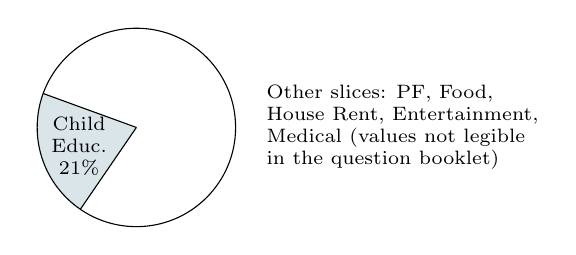
\begin{tikzpicture}[scale=0.9]
\fill[brand!15] (0,0) -- (160:1.4) arc (160:235.6:1.4) -- cycle;
\draw (0,0) circle (1.4);
\draw (0,0) -- (160:1.4); \draw (0,0) -- (235.6:1.4);
\node[font=\scriptsize,align=center] at (198:0.85) {Child\\Educ.\\21\%};
\node[font=\scriptsize,align=left,right] at (1.7,0) {Other slices: PF, Food,\\House Rent, Entertainment,\\Medical (values not legible\\in the question booklet)};
\end{tikzpicture}}
\optsfour{38662}{38862}{38962}{38752}
\dropped{}
\begin{explain}
Only the \emph{Child Education = 21\%} slice was legibly printed. The PF and house-rent percentages, which are needed to answer, could not be read from the chart, so the question could not be solved and the agency \textbf{dropped} it.
For reference, the options are about 70\% of the income: $0.70\times55{,}660=38{,}962$ (option C). This would be the answer if PF and house rent together formed 30\% of expenditure.
\end{explain}
\end{question}

\begin{question}{22}
{Choose the graph that best fits with this statement: "House prices rose in January and February, fell slightly in March and are now holding steady".\par}
\optsfour{\tikz[baseline=3mm,scale=0.45]{\draw[->](0,0)--(2.6,0);\draw[->](0,0)--(0,1.6);\draw[thick,brand](0,1)--(1.8,1);}}{\tikz[baseline=3mm,scale=0.45]{\draw[->](0,0)--(2.6,0);\draw[->](0,0)--(0,1.6);\draw[thick,brand](0,0.8) .. controls (1.2,0.8) and (1.8,1) .. (2,1.5);}}{\tikz[baseline=3mm,scale=0.45]{\draw[->](0,0)--(2.6,0);\draw[->](0,0)--(0,1.6);\draw[thick,brand](0,0)--(1.9,1.5);}}{\tikz[baseline=3mm,scale=0.45]{\draw[->](0,0)--(2.6,0);\draw[->](0,0)--(0,1.6);\draw[thick,brand](0,0.6) .. controls (0.4,1.3) and (0.6,1.4) .. (0.9,0.9) .. controls (1.1,0.6) and (1.3,0.9) .. (1.6,0.95) -- (2.3,0.95);}}
\answer{D}{\tikz[baseline=3mm,scale=0.45]{\draw[->](0,0)--(2.6,0);\draw[->](0,0)--(0,1.6);\draw[thick,brand](0,0.6) .. controls (0.4,1.3) and (0.6,1.4) .. (0.9,0.9) .. controls (1.1,0.6) and (1.3,0.9) .. (1.6,0.95) -- (2.3,0.95);}}
\begin{explain}
The statement has three phases. Prices \textbf{rise} (January--February), then \textbf{fall slightly} (March), then stay \textbf{steady} (now). Only graph (D) shows a rise, a small dip and then a flat line.
\why{(A) is flat throughout; (B) and (C) keep rising, with (B) accelerating and (C) at a constant rate.}
\end{explain}
\end{question}

\begin{question}{23}
{A researcher uses systematic random sampling from a company directory that has 500 employees listed in alphabetical order. If the desired samples size is 20, and the first name to be selected is number 9, which of the following will not be selected ?\par}
\optsfour{89}{134}{309}{484}
\answer{A}{89}
\begin{explain}
Sampling interval $k=\dfrac{N}{n}=\dfrac{500}{20}=25$. Selected numbers: $9, 34, 59, 84, 109, 134, \ldots, 309, \ldots, 484$, i.e.\ $9+25m$.
\begin{itemize}
\item $134=9+25\times5$ \checkmark, $309=9+25\times12$ \checkmark, $484=9+25\times19$ \checkmark
\item $89-9=80$ is not a multiple of 25, so \textbf{89 is not selected}.
\end{itemize}
\end{explain}
\end{question}

\begin{question}{24}
{The bar graph given below shows the Foreign Exchange Reserves of a Country (in millions US\$) from 1991-92 to 1998-99. The ratio of the number of years in which the foreign exchange reserves are above the average reserves, to those in which the reserves are below the average reserves is\par}
\qfigure{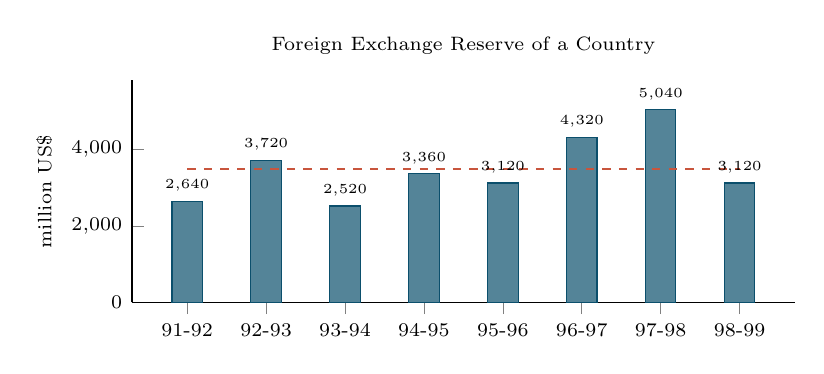
\begin{tikzpicture}
\begin{axis}[ybar,width=10cm,height=4.4cm,bar width=11pt,ymin=0,ymax=5800,
  symbolic x coords={91-92,92-93,93-94,94-95,95-96,96-97,97-98,98-99},xtick=data,
  nodes near coords,every node near coord/.append style={font=\tiny},
  tick label style={font=\scriptsize},ylabel={\scriptsize million US\$},
  title={\scriptsize Foreign Exchange Reserve of a Country},axis x line*=bottom,axis y line*=left]
\addplot[fill=brand!70,draw=brand] coordinates {(91-92,2640) (92-93,3720) (93-94,2520) (94-95,3360) (95-96,3120) (96-97,4320) (97-98,5040) (98-99,3120)};
\draw[accent,dashed,thick] (axis cs:91-92,3480) -- (axis cs:98-99,3480);
\end{axis}
\end{tikzpicture}}
\optsfour{2:6}{3:4}{3:5}{4:4}
\answer{C}{3:5}
\begin{explain}
\[\text{Average}=\frac{2640+3720+2520+3360+3120+4320+5040+3120}{8}=\frac{27840}{8}=3480\]
Above the average (dashed line): 3720, 4320 and 5040, which is \textbf{3 years}. Below: 2640, 2520, 3360, 3120 and 3120, which is \textbf{5 years}. The ratio is \textbf{3 : 5}.
\end{explain}
\end{question}

\begin{question}{25}
{What is the major purpose of Data Interpretation?\par}
\optsone{Getting meaning from the data and arriving as a conclusion}{Classification of data}{Analysis of data using suitable statistical tool}{Comparing different classified data}
\answer{A}{Getting meaning from the data and arriving as a conclusion}
\begin{explain}
\textbf{Data interpretation} means drawing meaning from analysed data, relating it to the research questions or hypotheses and \textbf{arriving at conclusions}. Classification, statistical analysis and comparison are \emph{earlier} steps that interpretation builds upon.
\end{explain}
\end{question}

\begin{question}{26}
{The main objective of formative evaluation\par}
\optsone{To find out the difficulties in learning}{To enhance students' learning}{To promote students to the next class}{To develop cooperation among students}
\answer{B}{To enhance students' learning}
\begin{explain}
\textbf{Formative evaluation} (Michael Scriven, 1967) is carried out \emph{during} instruction to give continuous feedback, so that teaching can be adjusted and \textbf{students' learning improved}. It is assessment \emph{for} learning.
\why{Identifying learning difficulties is \emph{diagnostic} evaluation; promotion to the next class is based on \emph{summative} evaluation.}
\end{explain}
\end{question}

\begin{question}{27}
{Which of the following options is not befitting to online teaching concept ?\par}
\optstwo{Swayamprabha}{Massive Open Online Courses}{Shodh Ganga}{Google meet}
\answer{C}{Shodh Ganga}
\begin{explain}
\textbf{Shodhganga} (INFLIBNET) is a digital \emph{repository of Indian PhD theses}; it is not an online teaching platform.
\why{SWAYAM Prabha (educational DTH), MOOCs and Google Meet (live classes) are all used for online or distance teaching.}
\end{explain}
\end{question}

\begin{question}{28}
{Which of the following statements about individual differences are true ?\newline 1. Every child is unique and different from each other.\newline 2. The same level of intelligence, the achievement level of student may be different.\newline 3. Heredity and environment both are the reason for individual differences.\newline 4. Individual differences are related to psychology only.\newline 5. Individual differences are there but it does not make any difference.\par}
\optsfour{1, 2 and 3}{1, 2 and 4}{2, 3 and 5}{3, 4 and 5}
\answer{A}{1, 2 and 3}
\begin{explain}
True statements:
\begin{itemize}
\item every child is unique (1);
\item students of the same intelligence may achieve differently, because of motivation, study habits and so on (2);
\item heredity and environment together cause individual differences (3).
\end{itemize}
Statement 4 is wrong because differences are physical, social and emotional as well as psychological. Statement 5 is wrong because differences do affect learning and teaching. The answer is 1, 2 and 3.
\end{explain}
\end{question}

\begin{question}{29}
{One of your student remains quite in the class discussion while he/she is very talkative and playful outside the class, what would you do?\newline 1. Try to find why he/she remains quite in the class discussion and talk to him/her.\newline 2. Assign him/her some topic to speak in the class.\newline 3. You will ask question to the student so he/she has to speak.\newline 4. Let him/her be quite as it is his/her nature.\newline 5. Send him/her to playground and let him play where he/she is comfortable.\par}
\optsfour{1, 2 and 3}{2, 3 and 4}{1, 3 and 5}{2, 4 and 5}
\answer{A}{1, 2 and 3}
\begin{explain}
A good teacher (i) finds out \emph{why} the student is quiet in class and talks to him or her, (ii) gives the student a topic to present so as to build confidence, and (iii) involves the student by asking questions. Leaving the student alone (4) or sending the student to play (5) neglects the teacher's responsibility. The answer is 1, 2 and 3.
\end{explain}
\end{question}

\begin{question}{30}
{Bright student causes disturbance in showing of his/her knowledge while you are teaching, what would you do ?\newline 1. Give him/her some work that he can not do so he realise that he/she doesn't know everything.\newline 2. Give him/her some difficult work in the area of his/her interest.\newline 3. Give him/her some books to read in the area of his/her interest.\newline 4. You will connect his/her points in your talk.\newline 5. Complain against him/her to his/her parents.\par}
\optsfour{1, 2 and 4}{2, 4 and 5}{2, 3 and 5}{2, 3 and 4}
\answer{D}{2, 3 and 4}
\begin{explain}
Constructive handling of a bright student who disrupts class: set challenging work in the area of interest (2), suggest enrichment reading (3), and connect the student's points with the lesson so the contribution is valued (4).
Setting impossible work to humiliate the student (1) or complaining to the parents (5) is negative. The answer is 2, 3 and 4.
\end{explain}
\end{question}

\begin{question}{31}
{Deep Ecology has focused upon\newline a. Ecosophy\newline b. Sustainable life style\newline c. Richness and diversity of life\newline d. Deforestation\newline e. Only abiotic ecosystem\newline Choose the correct option given below.\par}
\optstwo{Options b, d and e are correct}{Options a, c and b are correct}{Options a, b and e are correct}{Options b, c and e are correct}
\answer{B}{Options a, c and b are correct}
\begin{explain}
\textbf{Deep ecology} (Arne Naess, 1973) holds that all living beings have intrinsic value. It emphasises \textbf{ecosophy} (ecological wisdom or harmony), \textbf{richness and diversity of life}, and a \textbf{simple, sustainable lifestyle}. It is not limited to the abiotic ecosystem. The answer is a, b and c.
\end{explain}
\end{question}

\begin{question}{32}
{As per the latest report on 'All India Survey on Higher Education (2019-2020)', the Gender Parity Index in India is\par}
\optsfour{1.01}{1.02}{1.11}{1.21}
\answer{A}{1.01}
\begin{explain}
According to \textbf{AISHE 2019--20}, the \textbf{Gender Parity Index (GPI)} in higher education was \textbf{1.01}. This was the first time that female GER exceeded male GER. Total GER was 27.1\%.
\end{explain}
\end{question}

\begin{question}{33}
{Higher Education 4.0 has emphasized more upon\par}
\optstwo{Synchronous learning}{Blended mode of learning}{Face to face learning}{Adult and continuing learning}
\answer{B}{Blended mode of learning}
\begin{explain}
\emph{Higher Education 4.0}, aligned with Industry 4.0, promotes technology-integrated, flexible, personalised learning. It stresses \textbf{blended learning}, combining online and face-to-face modes.
\end{explain}
\end{question}

\begin{question}{34}
{Match the following given in List--I and List--II and select the correct option given below.\\[2pt]
\begin{tabular}{@{}p{0.3\linewidth}p{0.62\linewidth}@{}}
\textbf{List--I} & \textbf{List--II}\\
1. National Digital Library & a. Plenty of international electronic journals and e-books are made available to all HEIs\\
2. National Academic Depository & b. To incorporate Robotics in Engineering Education\\
3. e-Yantra & c. To facilitate digital issuance, storage, access and verification of Academic credentials\\
4. e-Shodh Sindhu & d. To develop a framework of virtual repository of learning resources with a single window search facility\\
\end{tabular}\par}
\optstwo{1-d, 2-b, 3-a, 4-c}{1-d, 2-a, 3-c, 4-b}{1-b, 2-c, 3-d, 4-a}{1-d, 2-c, 3-b, 4-a}
\answer{D}{1-d, 2-c, 3-b, 4-a}
\begin{explain}
\begin{itemize}
\item \textbf{National Digital Library of India} (IIT Kharagpur): a virtual repository of learning resources with single-window search, so 1-d.
\item \textbf{National Academic Depository (NAD)}: digital issue, storage, access and verification of academic awards, so 2-c.
\item \textbf{e-Yantra} (IIT Bombay): brings robotics into engineering education, so 3-b.
\item \textbf{e-ShodhSindhu} (INFLIBNET): e-journals and e-books for HEIs, so 4-a.
\end{itemize}
\end{explain}
\end{question}

\begin{question}{35}
{Which of the following core principle has not been mentioned in National Education Policy 2020?\par}
\optstwo{Extensive use of Technology}{Respect for Global Diversity}{Synergy in curriculum}{Creativity and critical thinking}
\answer{B}{Respect for Global Diversity}
\begin{explain}
The fundamental principles in NEP~2020 include extensive use of technology, creativity and critical thinking, multidisciplinarity and a holistic approach (synergy in curriculum), and ``respect for diversity and respect for the local context''. \textbf{``Respect for global diversity''} is not among the stated principles.
\end{explain}
\end{question}

\begin{question}{36}
{Match Section--I with Section--II.\\[2pt]
\begin{tabular}{@{}ll@{}}
\textbf{Section--I} & \textbf{Section--II}\\
1. Haptics & a. Use of body movement\\
2. Proxemics & b. Use of space and effects\\
3. Paralanguage & c. Communication through touching\\
4. Kinesics & d. Use of pitch and volume of voice\\
\end{tabular}\par}
\optstwo{1-a, 2-b, 3-c, 4-d}{1-b, 2-a, 3-d, 4-c}{1-c, 2-d, 3-a, 4-b}{1-c, 2-b, 3-d, 4-a}
\answer{D}{1-c, 2-b, 3-d, 4-a}
\begin{explain}
Haptics is touch (1-c); Proxemics is space (2-b); Paralanguage covers pitch, volume, tone and rate of voice (3-d); Kinesics is body movement (4-a). The match is 1-c, 2-b, 3-d, 4-a.
\end{explain}
\end{question}

\begin{question}{37}
{Which of the following are the example of communicative tool?\newline 1. Teleconferencing\newline 2. Voice mail\newline 3. Chat\newline 4. Multimedia Encyclopedia\par}
\optsfour{1, 3 and 4}{1, 2 and 3}{1, 2 and 4}{2, 3 and 4}
\answer{B}{1, 2 and 3}
\begin{explain}
Teleconferencing, voice mail and chat are \textbf{communication tools}: they carry messages between people, synchronously or asynchronously. A \textbf{multimedia encyclopaedia} is an information or reference resource, not a communication tool. The answer is 1, 2 and 3.
\end{explain}
\end{question}

\begin{question}{38}
{Which is not a characteristics of Effective Communication?\par}
\optstwo{Completeness}{Cultural heterogeneity}{Concreteness}{Correctness}
\answer{B}{Cultural heterogeneity}
\begin{explain}
The \textbf{7 Cs of effective communication} are Clarity, Conciseness, Concreteness, Correctness, Coherence, Completeness and Courtesy (some versions add Consideration). \textbf{Cultural heterogeneity} is not one of them; cultural differences are in fact a potential \emph{barrier}.
\end{explain}
\end{question}

\begin{question}{39}
{Which of the following is not a component of a communication system ?\par}
\optsfour{Sender}{Message}{Feedback}{Reinforcement}
\answer{D}{Reinforcement}
\begin{explain}
The components of a communication system are \textbf{sender (source), message, encoding, channel, receiver, decoding and feedback}, along with noise and context. \textbf{Reinforcement} is a learning-theory concept (Skinner), not a component of communication.
\end{explain}
\end{question}

\begin{question}{40}
{What are the causes of semantic barriers in communication ?\newline 1. Poorly expressed message\newline 2. Use of technical language\newline 3. Unnatural assumption\newline 4. Lack of attention\par}
\optsfour{2, 3, 4}{1, 2, 3}{1, 3, 4}{1, 2, 4}
\answer{B}{1, 2, 3}
\begin{explain}
\textbf{Semantic barriers} are barriers of \emph{meaning}. They include a badly expressed message (1), technical language or jargon (2), and unclarified or wrong assumptions (3). \textbf{Lack of attention} (4) is a \emph{psychological} barrier. The answer is 1, 2 and 3.
\end{explain}
\end{question}

\begin{question}{41}
{Given below are two statements - One is labeled as Assertion (A) and the other is labeled as Reason (R).\newline Assertion (A): Government of India has established higher educational bodies to ensure the quality of education.\newline Reason (R): There are some educational institutions in India which do not provide quality education.\newline In the context of the above two statements, choose the correct option.\par}
\optsone{Both (A) and (R) are true and (R) is the correct explanation of (A)}{Both (A) and (R) are true but (R) is not the correct explanation of (A)}{(A) is true, but (R) is false}{(A) is false, but (R) is true}
\answer{A}{Both (A) and (R) are true and (R) is the correct explanation of (A)}
\begin{explain}
The Government has set up regulatory and quality-assurance bodies (UGC, AICTE, NAAC, NBA, NCTE and others) because some institutions fall short on quality. The Reason gives exactly why these bodies were established, so both are true and R explains A.
\end{explain}
\end{question}

\begin{question}{42}
{Which of the following statements are true in the context of Vyapti?\newline 1. It is the relation between middle and major term in the logical ground of inference.\newline 2. It means a state of pervasion.\newline 3. Vyapti serves a basis of Nyaya syllogism.\par}
\optsfour{1 and 2}{2 and 3}{1 and 3}{1, 2 and 3}
\answer{D}{1, 2 and 3}
\begin{explain}
In Nyaya logic, \textbf{Vyapti} (invariable concomitance) is:
\begin{itemize}
\item the relation between the \emph{middle term} (hetu, e.g.\ smoke) and the \emph{major term} (sadhya, e.g.\ fire) (1);
\item literally a state of \emph{pervasion}, in which smoke is pervaded by fire (2);
\item the logical basis of inference and hence of the Nyaya syllogism, expressed in its \emph{Udaharana} step (3).
\end{itemize}
All three statements are true.
\end{explain}
\end{question}

\begin{question}{43}
{Find the next term of given series.\newline ATTRIBUTION, TTRIBUTIO, RIBUTIO, IBUTI.\ldots{}?\par}
\optsfour{BUT}{UTI}{UT}{IBU}
\answer{B}{UTI}
\begin{explain}
Letters are removed alternately from both ends and from the front:
\begin{center}
ATTRIBUTION $\xrightarrow{\text{drop 1st \& last}}$ TTRIBUTIO $\xrightarrow{\text{drop first 2}}$ RIBUTIO $\xrightarrow{\text{drop 1st \& last}}$ IBUTI $\xrightarrow{\text{drop first 2}}$ \textbf{UTI}
\end{center}
\end{explain}
\end{question}

\begin{question}{44}
{In a certain relationship\newline $S\times T$ means S is brother of T\newline S-T means S is mother of T\newline $S+T$ means S is father of T\newline Answer the following question based on data above.\newline In the pattern $M+N+O$ how is M related to O?\par}
\optsfour{Uncle}{Father}{Cousin}{Grandfather}
\answer{D}{Grandfather}
\begin{explain}
$M+N$: M is the father of N. $N+O$: N is the father of O. So M is the father of O's father, i.e.\ O's \textbf{grandfather}.
\end{explain}
\end{question}

\begin{question}{45}
{Which of the following diagrams indicates the best relation between Travelers, Train and Bus?\par}
\optsfour{\tikz[baseline=-0.5ex,scale=0.3]{\draw (0,0) circle(1.2); \draw (0,0) circle(0.6); \draw (2.2,0) ellipse(0.6 and 0.4);}}{\tikz[baseline=-0.5ex,scale=0.3]{\draw (0,0.5) circle(0.7); \draw (1.3,0.5) circle(0.7); \draw (0.65,-0.6) circle(0.7);}}{\tikz[baseline=-0.5ex,scale=0.3]{\draw (0,0) circle(1.3); \draw (-0.55,0) circle(0.5); \draw (0.55,0) circle(0.5);}}{\tikz[baseline=-0.5ex,scale=0.3]{\draw (0,0) circle(0.8); \draw (1.1,0) circle(0.8); \draw (2.2,0) circle(0.8);}}
\answer{C}{\tikz[baseline=-0.5ex,scale=0.3]{\draw (0,0) circle(1.3); \draw (-0.55,0) circle(0.5); \draw (0.55,0) circle(0.5);}}
\begin{explain}
In the official answer, \textbf{Travellers} is the large set, and the two means of travel, \textbf{train} (train travellers) and \textbf{bus} (bus travellers), are two separate groups inside it. They are shown as two disjoint circles, since a journey is made by one or the other, within one big circle. This is diagram (C).
\begin{center}
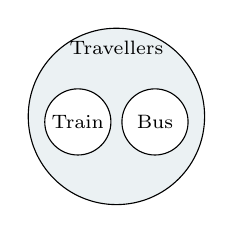
\begin{tikzpicture}[scale=0.7,font=\scriptsize]
\draw[fill=brand!8] (0,0) circle(1.6); \node at (0,1.25) {Travellers};
\draw[fill=white] (-0.7,-0.1) circle(0.6) node {Train}; \draw[fill=white] (0.7,-0.1) circle(0.6) node {Bus};
\end{tikzpicture}
\end{center}
\end{explain}
\end{question}

\begin{question}{46}
{How an achievement test is different from Entrance test ?\par}
\optsone{Achievement test needs high content validity whereas Entrance test needs high construct validity.}{Achievement test needs high construct validity whereas Entrance test needs high content validity.}{Achievement test needs high predictive validity whereas Entrance test needs high content validity.}{Achievement test needs high content validity whereas Entrance test needs high predictive validity.}
\answer{D}{Achievement test needs high content validity whereas Entrance test needs high predictive validity.}
\begin{explain}
An \textbf{achievement test} measures how well the content taught has been learnt, so it must have high \textbf{content validity} (it must sample the syllabus adequately). An \textbf{entrance test} is used to predict future success in a course, so it must have high \textbf{predictive validity}.
\end{explain}
\end{question}

\begin{question}{47}
{Sequential use of the three levels of coding - open coding, selective coding and theoretical coding is done in\par}
\optstwo{Phenomenological research}{Ethnographic research}{Grounded theory research}{Case study research}
\answer{C}{Grounded theory research}
\begin{explain}
The sequence \emph{open coding $\rightarrow$ selective coding $\rightarrow$ theoretical coding} belongs to Glaser's version of \textbf{grounded theory}. Strauss and Corbin's version uses open $\rightarrow$ axial $\rightarrow$ selective coding. In both, theory is generated from data by constant comparison.
\end{explain}
\end{question}

\begin{question}{48}
{In a reaction scale, the scale values are from 0 to 5. Which of the following scales of measurement is applicable for the data collected by this scale ?\par}
\optsfour{Nominal scale}{Ordinal scale}{Interval scale}{Ratio scale}
\answer{C}{Interval scale}
\begin{explain}
A reaction (rating) scale scored 0--5 has equal intervals between successive points. In educational research such summated rating data are treated as \textbf{interval-scale} data, which allows means and standard deviations to be computed. The official key accepts this answer.
\tip{Scales: Nominal (names or categories), Ordinal (rank order), Interval (equal intervals, arbitrary zero), Ratio (equal intervals with a true zero).}
\end{explain}
\end{question}

\begin{question}{49}
{Which of the following is a normal group ?\par}
\optsone{Skewness is zero and it is Platykurtic}{Mean = Median = Mode and it is Leptokurtic}{Mean = Median = Mode and it is Platykurtic}{Skewness is zero and it is Mesokurtic}
\answer{D}{Skewness is zero and it is Mesokurtic}
\begin{explain}
A \textbf{normal distribution} is perfectly symmetrical (\textbf{skewness $=0$}, mean $=$ median $=$ mode) and has \textbf{mesokurtic} peakedness (kurtosis $=3$, or excess kurtosis $=0$).
\why{Leptokurtic curves are more peaked and platykurtic curves flatter than normal.}
\end{explain}
\end{question}

\begin{question}{50}
{The transformation of human mind from theological metaphysical to a rational and scientific belief led to the emergence of\par}
\optstwo{Holism}{Rationalism}{Critical consciousness}{Positivism}
\answer{D}{Positivism}
\begin{explain}
Auguste Comte's \emph{Law of Three Stages} holds that human thought passes from the \textbf{theological} to the \textbf{metaphysical} and then to the \textbf{positive (scientific)} stage. This transformation to rational, scientific thinking gave rise to \textbf{Positivism}, the philosophy that only knowledge verified through observation and the scientific method is valid.
\end{explain}
\end{question}

\paperchapter{December 2021}{23 January 2022}{A}{50}{15th GSET}
\keytable{\kcell{1}{A} & \kcell{2}{A} & \kcell{3}{B} & \kcell{4}{B} & \kcell{5}{C} & \kcell{6}{B} & \kcell{7}{D} & \kcell{8}{B} & \kcell{9}{C} & \kcell{10}{A} \\
\kcell{11}{B} & \kcell{12}{B} & \kcell{13}{B} & \kcell{14}{B} & \kcell{15}{A} & \kcell{16}{B} & \kcell{17}{A} & \kcell{18}{C} & \kcell{19}{C} & \kcell{20}{B} \\
\kcell{21}{B} & \kcell{22}{A} & \kcell{23}{D} & \kcell{24}{D} & \kcell{25}{D} & \kcell{26}{C} & \kcell{27}{B} & \kcell{28}{A} & \kcell{29}{B} & \kcell{30}{D} \\
\kcell{31}{B} & \kcell{32}{C} & \kcell{33}{C} & \kcell{34}{D} & \kcell{35}{C} & \kcell{36}{A} & \kcell{37}{D} & \kcell{38}{D} & \kcell{39}{C} & \kcell{40}{C} \\
\kcell{41}{C} & \kcell{42}{D} & \kcell{43}{D} & \kcell{44}{B} & \kcell{45}{D} & \kcell{46}{C} & \kcell{47}{C} & \kcell{48}{C} & \kcell{49}{A} & \kcell{50}{D}}
\begin{question}{1}
{Identify which of the following steps are carried out for constant comparison in grounded theory research?\par}
\optsone{Data collection, note taking, coding and memoing}{Data collection, data reduction, data display, conclusion drawing and verification}{Data collection, axial coding, categorization and narrative description}{Data collection, contrasting, comparing and generating themes and patterns}
\answer{A}{Data collection, note taking, coding and memoing}
\begin{explain}
In \textbf{grounded theory} (Glaser \& Strauss, 1967) the \emph{constant comparative method} runs as a cycle. The researcher \textbf{collects data}, takes \textbf{field notes}, \textbf{codes} the data (open, axial and selective coding) and writes \textbf{memos}, comparing each new piece of data with earlier codes and categories until theoretical saturation is reached.
\why{(B) is Miles \& Huberman's interactive model of qualitative analysis; (C) mixes coding with narrative description; (D) describes generic thematic analysis.}
\end{explain}
\end{question}

\begin{question}{2}
{Which of the following is common in all true experimental and Quasi experimental designs?\par}
\optstwo{Control group}{Randomization}{Pre-testing and post-testing}{Pre-testing}
\answer{A}{Control group}
\begin{explain}
True experimental designs always have a \emph{control group} and random assignment. Quasi-experimental designs (e.g.\ the non-equivalent control group design) \emph{lack randomization} but still compare treated units with a control or comparison group. The common element, as per the official key, is the \textbf{control group}.
\why{Randomization is absent in quasi-experiments, and pre-testing is not used in every design (e.g.\ the post-test-only control group design).}
\end{explain}
\end{question}

\begin{question}{3}
{Find the wrong term in the letter-number series given below.\newline G4T, J10R, M20P, P43N, S90L\par}
\optsfour{G4T}{J10R}{M20P}{P43N}
\answer{B}{J10R}
\begin{explain}
\begin{itemize}
\item Letters: G, J, M, P, S (+3) and T, R, P, N, L ($-2$) are both regular.
\item Numbers should follow $\times2+1, \times2+2, \times2+3, \times2+4$: $4\rightarrow\mathbf{9}\rightarrow20\rightarrow43\rightarrow90$.
\end{itemize}
The second term should be J\textbf{9}R, so \textbf{J10R} is wrong.
\end{explain}
\end{question}

\begin{question}{4}
{A cube whose each corner is named as A, B, C, D, F, G and H is segmented into 27 equal tiny cubes. Before dividing the cube, each face of its varnished with different colours. How many tiny cubes will be formed having more than one colour?\par}
\optsfour{64}{20}{55}{53}
\answer{B}{20}
\begin{explain}
A cube cut into $3\times3\times3=27$ small cubes, with each face painted a different colour:
\begin{itemize}
\item corner cubes have 3 colours: \textbf{8};
\item edge (middle-of-edge) cubes have 2 colours: $12\times(3-2)=\mathbf{12}$;
\item face-centre cubes have 1 colour: 6; the central cube has none: 1.
\end{itemize}
Cubes with more than one colour $=8+12=\mathbf{20}$.
\end{explain}
\end{question}

\begin{question}{5}
{Which of the following is not true in relation to 'SWAYAM'?\par}
\optsone{It is Sanskrit acronym that stands for 'Study Webs of Active-Learning for Young Aspiring Minds'}{It is an Indian Massive Open Online Course (MOOC) platform}{It has been developed jointly by MHRD (now MoE) and UGC with the help of Infosys}{It is under 'Digital India' to give a coordinated stage and free entry to web courses covering all advance education and skill sector courses}
\answer{C}{It has been developed jointly by MHRD (now MoE) and UGC with the help of Infosys}
\begin{explain}
SWAYAM was developed by \textbf{MHRD (now MoE) and AICTE with the help of Microsoft}, not by UGC with Infosys. So statement (C) is not true. The other statements are correct: SWAYAM stands for \emph{Study Webs of Active-Learning for Young Aspiring Minds}, is India's MOOC platform, and was launched under Digital India.
\end{explain}
\end{question}

\begin{question}{6}
{Which of the following are game based learning platforms?\newline a. Kahoot\newline b. Socrative\newline c. Quizizz\newline d. e-PG Pathshala\newline e. Edmodo\par}
\optsfour{e, d and b}{a, b and c}{a, c and d}{c, e and a}
\answer{B}{a, b and c}
\begin{explain}
\textbf{Kahoot}, \textbf{Socrative} and \textbf{Quizizz} are game-based, quiz-style learning and assessment platforms with points, leaderboards and timers.
\why{e-PG Pathshala is a UGC/INFLIBNET e-content repository for postgraduate subjects; Edmodo is a learning-management and social-classroom platform.}
\end{explain}
\end{question}

\begin{question}{7}
{In a certain relationship\newline $M/N$ means M is daughter of N\newline $M+N$ means M is father of N\newline M-N means M is mother of N\newline Answer the following question based on data above.\newline In the pattern $F^{*}G/H-I$, how is I related to G?\par}
\optsfour{Mother}{Sister}{Niece}{No relation}
\answer{D}{No relation}
\begin{explain}
$G/H$: G is the daughter of H. $H-I$: H is the mother of I. So I is a child of H, i.e.\ a sibling of G. The symbol ``$*$'' in $F*G$ is not defined in the code, and I's gender is not given, so ``Sister'' cannot be concluded. Mother and niece are clearly wrong. The official key gives \textbf{(D) No relation} (i.e.\ none of the definite relations offered can be established).
\end{explain}
\end{question}

\begin{question}{8}
{In the following figure triangle represents 'girls', square 'players' and circle 'coach'. Which part of the diagram represents the girls are player but not coach?\par}
\qfigure{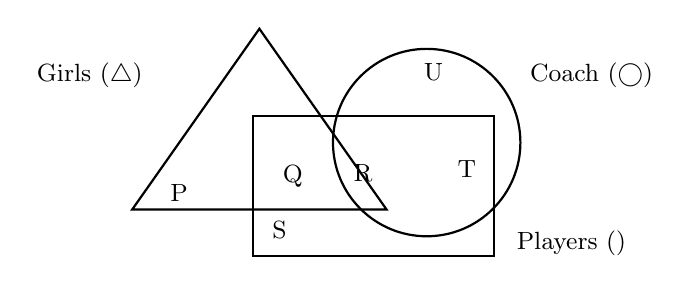
\begin{tikzpicture}[scale=0.85,font=\small]
\draw[thick] (-1.6,-0.5) -- (0.3,2.2) -- (2.2,-0.5) -- cycle;
\draw[thick] (0.2,-1.2) rectangle (3.8,0.9);
\draw[thick] (2.8,0.5) circle (1.4);
\node at (-0.9,-0.25) {P}; \node at (0.8,0) {Q}; \node at (1.85,0.05) {R}; \node at (0.6,-0.8) {S}; \node at (2.9,1.55) {U}; \node at (3.4,0.1) {T};
\node[left] at (-1.3,1.5) {Girls ($\triangle$)}; \node[right] at (4.2,1.5) {Coach ($\bigcirc$)}; \node[right] at (4.0,-1.0) {Players ($\square$)};
\end{tikzpicture}}
\optsfour{P}{Q}{R}{S}
\answer{B}{Q}
\begin{explain}
Girls who are players but not coaches lie \textbf{inside the triangle and inside the square but outside the circle}. That region is \textbf{Q}.
\why{P = girls only; R = girls who are players \emph{and} coaches; S = players only (not girls).}
\end{explain}
\end{question}

\begin{question}{9}
{If a student ask you a question whose answer is not known to you, then\newline 1. Give this question as a homework and start teaching.\newline 2. Tell him this question will be answered the next day.\newline 3. Ask him to come later and then send him to library.\newline 4. After the class you will go to library and try to find the answer.\newline 5. Appreciate the question and accept that you don't have information right now.\par}
\optsfour{1, 2 and 4}{3, 4 and 5}{2, 4 and 5}{2, 3 and 5}
\answer{C}{2, 4 and 5}
\begin{explain}
A good teacher is honest and a model learner: \textbf{appreciates the question and admits not knowing (5)}, \textbf{consults the library after class (4)} and \textbf{answers it the next day (2)}. Giving it as homework to hide ignorance (1) or sending the student away (3) is inappropriate. The answer is 2, 4 and 5.
\end{explain}
\end{question}

\begin{question}{10}
{Which of the following is most applicable to split half method of finding reliability ?\par}
\optsone{It shows the internal consistency of the test}{It shows the internal consistency of half of the test}{It can be used for tests having both subjective and objective type questions}{It can be used for tests with any number of items}
\answer{A}{It shows the internal consistency of the test}
\begin{explain}
In the \textbf{split-half method} one test is divided into two comparable halves (e.g.\ odd and even items), the two half-scores are correlated, and the result is stepped up with the Spearman--Brown formula $r_{tt}=\frac{2r_{hh}}{1+r_{hh}}$. It measures the \textbf{internal consistency of the whole test}.
\why{It needs a sufficiently large, even number of homogeneous items that can be split, and is unsuitable for speed tests.}
\end{explain}
\end{question}

\begin{question}{11}
{Match the List--I with List--II and choose the correct option given below.\\[2pt]
\begin{tabular}{@{}p{0.44\linewidth}p{0.5\linewidth}@{}}
\textbf{List--I} & \textbf{List--II}\\
1. National Institute of Educational Planning and Administration (NIEPA) & a. Deemed to be a University, 1964, under Section 3 of UGC Act, 1956\\
2. Tata Institute of Social Sciences (TISS) & b. A Central University and An Institution of National Importance\\
3. Mahatma Gandhi Antarrashtriya Hindi Vishwavidyalaya (MGAHV) & c. A Central University, established by an Act of Parliament, Act No.~3 of 1997\\
4. Visva-Bharati & d. Deemed to be University, 2006, under Section 3 of UGC Act, 1956\\
\end{tabular}\par}
\optstwo{1-b, 2-a, 3-c, 4-d}{1-d, 2-a, 3-c, 4-b}{1-b, 2-d, 3-c, 4-a}{1-c, 2-b, 3-d, 4-a}
\answer{B}{1-d, 2-a, 3-c, 4-b}
\begin{explain}
\begin{itemize}
\item \textbf{NIEPA} (now NIEPA, New Delhi) became a deemed university in \textbf{2006}, so 1-d.
\item \textbf{TISS}, Mumbai (founded 1936) was declared deemed in \textbf{1964}, so 2-a.
\item \textbf{MGAHV}, Wardha was established by \textbf{Act No.~3 of 1997}, so 3-c.
\item \textbf{Visva-Bharati}, Santiniketan (founded by Tagore) is a central university and an \textbf{institution of national importance} (Visva-Bharati Act, 1951), so 4-b.
\end{itemize}
\end{explain}
\end{question}

\begin{question}{12}
{Which of the following is not an independent vertical of one umbrella institution i.e. Higher Education Commission of India (HECI) as proposed in NEP 2020?\par}
\optsone{National Higher Education Regulatory Council (NHERC)}{University Education Council (UEC)}{General Education Council (GEC)}{Higher Education Grants Council (HEGC)}
\answer{B}{University Education Council (UEC)}
\begin{explain}
NEP~2020 proposes the \textbf{Higher Education Commission of India (HECI)} with four independent verticals:
\begin{enumerate}
\item \textbf{NHERC}, the National Higher Education Regulatory Council (regulation);
\item \textbf{NAC}, the National Accreditation Council (accreditation);
\item \textbf{HEGC}, the Higher Education Grants Council (funding);
\item \textbf{GEC}, the General Education Council (standard setting).
\end{enumerate}
A ``University Education Council'' is not one of them.
\end{explain}
\end{question}

\begin{question}{13}
{In a certain code $E=P$, $Z=C,$ $N=O$ $K=B$, $C=Q$ $A=X$ $R=H$, $B=R.$ How will BREAK be written in the same code?\par}
\optsfour{RHPBX}{RHPXB}{RHPXC}{ROPXB}
\answer{B}{RHPXB}
\begin{explain}
Using the given code: B$\rightarrow$R, R$\rightarrow$H, E$\rightarrow$P, A$\rightarrow$X, K$\rightarrow$B.
BREAK $\rightarrow$ \textbf{RHPXB}.
\end{explain}
\end{question}

\begin{question}{14}
{A and B travels from point P to Q at $17~km/hr$ and $19~km/hr$. respectively. P is 72 km away from Q. B reaches Q first and returns immediately and meets A at R. What is the distance between Q and R?\par}
\optsfour{10 km}{4 km}{15 km}{36 km}
\answer{B}{4 km}
\begin{explain}
Until they meet, A and B together cover $PQ+QR+PR=2\times72=144$ km.
\[t=\frac{144}{17+19}=4\text{ h};\quad\text{B covers }19\times4=76\text{ km}=72+QR\ \Rightarrow\ QR=\mathbf{4\ km}\]
\end{explain}
\end{question}

\begin{question}{15}
{Match List - I with List - II and select the correct option given below.\par\smallskip\begin{tabularx}{\linewidth}{@{}>{\raggedright\arraybackslash}X>{\raggedright\arraybackslash}X@{}}\toprule
\textbf{List-I (Software)} & \textbf{List - II (Application)}\\\midrule
1. Mendeley & a. Quantitative data analysis\\
2. SPSS & b. Reference manager\\
3. Turnitin & c. Plagiarism check\\
4. Nvivo & d. Qualitative data analysis\\
\bottomrule\end{tabularx}\par\smallskip
\par}
\optstwo{1-b, 2-a, 3-c, 4-d}{1-d, 2-a, 3-c, 4-b}{1-c, 2-a, 3-b, 4-d}{1-c, 2-a, 3-d, 4-b}
\answer{A}{1-b, 2-a, 3-c, 4-d}
\begin{explain}
Mendeley is a \textbf{reference manager} (1-b); SPSS does \textbf{quantitative} analysis (2-a); Turnitin checks \textbf{plagiarism} (3-c); NVivo does \textbf{qualitative} analysis (4-d).
\end{explain}
\end{question}

\begin{question}{16}
{Which of the following statement/s is/are correct?\newline a. For the sequence of integers represented in binary 00111, 01001, 01011, P.\ldots{} the next integer P would be represented as 011101.\newline b. A byte is a binary number consisting of exactly 8 bits.\newline Choose the correct option:\par}
\optstwo{a only}{b only}{both a and b}{neither a nor b}
\answer{B}{b only}
\begin{explain}
(a) $00111=7$, $01001=9$, $01011=11$: odd numbers, so next is $13=\mathbf{01101}$, not $011101$ ($=29$). Statement (a) is false.
(b) A byte is exactly 8 bits. Statement (b) is true. So \textbf{b only}.
\end{explain}
\end{question}

\begin{question}{17}
{Study the chart and answer the question. The pie chart given here represents the domestic expenditure of a family in percent. If the total monthly income of the family is Rs.~55,660/-, the annual savings in the form of PF would be (in nearest Rs.)\par}
\qfigure{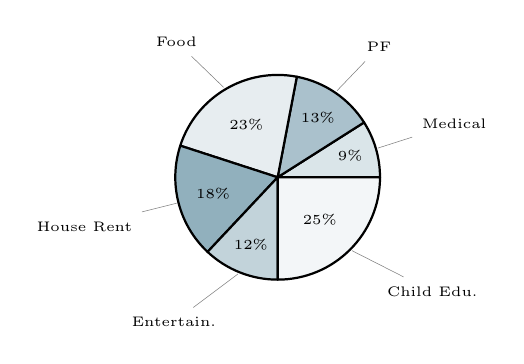
\begin{tikzpicture}[scale=1]
\pie[radius=1.3,text=pin,color={brand!15,brand!35,brand!10,brand!45,brand!25,brand!5},font=\tiny]{9/Medical,13/PF,23/Food,18/House Rent,12/Entertain.,25/Child Edu.}
\end{tikzpicture}}
\optsfour{86830}{86155}{96830}{76830}
\answer{A}{86830}
\begin{explain}
Monthly PF $=13\%\times55{,}660=7{,}235.80$.
Annual PF $=7{,}235.80\times12=86{,}829.6\approx$ \textbf{Rs.~86,830}.
\end{explain}
\end{question}

\begin{question}{18}
{Choose the graph that best fits with this statement: "This car has excellent acceleration".\par}
\optsfour{\tikz[baseline=3mm,scale=0.45]{\draw[->](0,0)--(2.6,0);\draw[->](0,0)--(0,1.6);\draw[thick,brand](0,1)--(1.8,1);}}{\tikz[baseline=3mm,scale=0.45]{\draw[->](0,0)--(2.6,0);\draw[->](0,0)--(0,1.6);\draw[thick,brand](0,0.8) .. controls (1.2,0.8) and (1.8,1) .. (2,1.5);}}{\tikz[baseline=3mm,scale=0.45]{\draw[->](0,0)--(2.6,0);\draw[->](0,0)--(0,1.6);\draw[thick,brand](0,0)--(1.9,1.5);}}{\tikz[baseline=3mm,scale=0.45]{\draw[->](0,0)--(2.6,0);\draw[->](0,0)--(0,1.6);\draw[thick,brand](0,0.6) .. controls (0.4,1.3) and (0.6,1.4) .. (0.9,0.9) .. controls (1.1,0.6) and (1.3,0.9) .. (1.6,0.95) -- (2.3,0.95);}}
\answer{C}{\tikz[baseline=3mm,scale=0.45]{\draw[->](0,0)--(2.6,0);\draw[->](0,0)--(0,1.6);\draw[thick,brand](0,0)--(1.9,1.5);}}
\begin{explain}
Plotting speed against time, excellent acceleration means the speed rises \textbf{quickly and steadily from rest}: a straight, steep line through the origin, as in graph (C).
\why{(A) shows constant speed (no acceleration); (B) starts with an almost flat curve (sluggish at first); (D) rises, falls and levels off.}
\end{explain}
\end{question}

\begin{question}{19}
{A group of students of your class face problem in learning, you want to identify the deficiencies and difficulties of the learner, which evaluation would you choose?\par}
\optstwo{Formative evaluation}{Summative evaluation}{Diagnostic evaluation}{Qualitative evaluation}
\answer{C}{Diagnostic evaluation}
\begin{explain}
\textbf{Diagnostic evaluation} identifies the specific learning difficulties and their causes, so that remedial teaching can follow.
\why{Formative evaluation monitors progress during teaching; summative evaluation certifies achievement at the end.}
\end{explain}
\end{question}

\begin{question}{20}
{What should be done to ensure optimum growth of the slow learner?\newline 1. They should be treated like others, they will grow themself.\newline 2. They should be given challenging task as per their level in the area of their interest.\newline 3. They should be left at their own.\newline 4. They should get sufficient resources.\newline 5. Regular activities regarding diagnosis and remedy.\par}
\optsfour{1, 3 and 5}{2, 4 and 5}{2, 3 and 4}{3, 4 and 5}
\answer{B}{2, 4 and 5}
\begin{explain}
Slow learners need \textbf{tasks matched to their level and interests (2)}, \textbf{sufficient resources (4)} and \textbf{regular diagnosis and remediation (5)}. Treating them like everyone else or leaving them on their own (1, 3) neglects their needs. The answer is 2, 4 and 5.
\end{explain}
\end{question}

\begin{question}{21}
{Which of the following is a lead agency for 'Education for Sustainable Development'?\par}
\optstwo{Brundtland Commission}{UNESCO}{UNDP}{UNICEF}
\answer{B}{UNESCO}
\begin{explain}
\textbf{UNESCO} is the lead UN agency for \textbf{Education for Sustainable Development (ESD)}. It led the UN Decade of ESD (2005--2014), the Global Action Programme (2015--2019) and now the \emph{ESD for 2030} framework.
\end{explain}
\end{question}

\begin{question}{22}
{The Global Education Development Agenda reflected in the Goal 4 (SDG4) of the 2030 Agenda for Sustainable Development, adopted by India in 2015, seeks to\par}
\optsone{"ensure inclusive and equitable quality education and promote lifelong learning opportunities for all" by 2030}{"ensure inclusive and affordable education and desired learning opportunities for all" by 2030}{"ensure accountable and quality education and promote creative learning opportunities for all" by 2030}{"ensure equity, equality, quality and promote lifelong learning opportunities for all" by 2030}
\answer{A}{"ensure inclusive and equitable quality education and promote lifelong learning opportunities for all" by 2030}
\begin{explain}
SDG~4 reads: ``\textbf{Ensure inclusive and equitable quality education and promote lifelong learning opportunities for all}'' by 2030.
\end{explain}
\end{question}

\begin{question}{23}
{A researcher uses systematic random sampling from a company directory that has 600 employees listed in alphabetical order. If the desired samples size is 30, and the first name to be selected is number 8, which of the following will not be selected?\par}
\optsfour{88}{368}{428}{558}
\answer{D}{558}
\begin{explain}
Interval $k=600/30=20$. The selected numbers are $8, 28, 48, \ldots$, i.e.\ $8+20m$.
$88=8+80$ \checkmark, $368=8+360$ \checkmark, $428=8+420$ \checkmark, but $558-8=550$ is not a multiple of 20. So \textbf{558 is not selected}.
\end{explain}
\end{question}

\begin{question}{24}
{The bar graph given below shows the Foreign Exchange Reserves of a Country (in millions US \$) from 1991-92 to 1998-99. The foreign exchange reserves in 1997-98 was how many times that in 1994-95.\par}
\qfigure{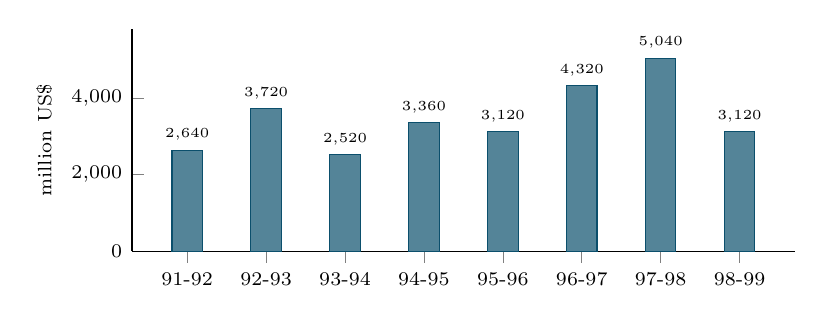
\begin{tikzpicture}
\begin{axis}[ybar,width=10cm,height=4.4cm,bar width=11pt,ymin=0,ymax=5800,
  symbolic x coords={91-92,92-93,93-94,94-95,95-96,96-97,97-98,98-99},xtick=data,
  nodes near coords,every node near coord/.append style={font=\tiny},
  tick label style={font=\scriptsize},ylabel={\scriptsize million US\$},
  axis x line*=bottom,axis y line*=left]
\addplot[fill=brand!70,draw=brand] coordinates {(91-92,2640) (92-93,3720) (93-94,2520) (94-95,3360) (95-96,3120) (96-97,4320) (97-98,5040) (98-99,3120)};
\end{axis}
\end{tikzpicture}}
\optsfour{0.7}{1.2}{1.4}{1.5}
\answer{D}{1.5}
\begin{explain}
\[\frac{\text{Reserves in 1997--98}}{\text{Reserves in 1994--95}}=\frac{5040}{3360}=\mathbf{1.5}\]
\end{explain}
\end{question}

\begin{question}{25}
{Which of the following is not a barrier of the Effective Communication?\par}
\optstwo{Poor ability to listen others}{Lack of transparency and trust}{Cultural and language differences}{Differences in economic status}
\answer{D}{Differences in economic status}
\begin{explain}
Poor listening, lack of trust and transparency, and cultural and language differences all hinder communication. A mere \textbf{difference in economic status} does not by itself prevent effective communication, so it is not a barrier in this list.
\end{explain}
\end{question}

\begin{question}{26}
{What are the major components of effective classroom communication?\newline 1. Sense of Humour\newline 2. Feedback\newline 3. Classroom cleanliness\newline 4. Body Language\newline 5. Safe Environment\par}
\optsfour{1, 2, 3, 4}{2, 3, 4, 5}{1, 2, 4, 5}{1, 3, 4, 5}
\answer{C}{1, 2, 4, 5}
\begin{explain}
Effective classroom communication depends on the teacher's \textbf{sense of humour} (1), continuous \textbf{feedback} (2), appropriate \textbf{body language} (4) and a psychologically \textbf{safe environment} (5). Classroom cleanliness is a physical-hygiene factor, not a component of communication. The answer is 1, 2, 4, 5.
\end{explain}
\end{question}

\begin{question}{27}
{A second commitment period of Kyoto protocol that was agreed to in 2012 to extend the agreement to 2020, known as the\par}
\optstwo{Paris Agreement}{Doha Amendment}{International Solar Alliance}{Environment Protection Act}
\answer{B}{Doha Amendment}
\begin{explain}
The \textbf{Doha Amendment} (COP18, Doha, December 2012) set up the \emph{second commitment period} of the Kyoto Protocol, from 2013 to 2020. (The first period ran 2008--2012.)
\why{The Paris Agreement (2015) is a separate treaty; the International Solar Alliance was launched by India and France in 2015; the Environment Protection Act is India's 1986 law.}
\end{explain}
\end{question}

\begin{question}{28}
{Which of the following Statement is true in relation to Agenda 21 of the Earth Summit in Rio de Janerio, Brazil 1992?\par}
\optsone{It was plan of action to be taken globally, nationally and locally in every area in which human impacts on the environment.}{It was planning for base-plan of Millennium Development Goals.}{It was planning for base-plan of Sustainable Development Goals.}{It was plan of action to be taken globally, nationally, locally in every area of gender disparity and inequality.}
\answer{A}{It was plan of action to be taken globally, nationally and locally in every area in which human impacts on the environment.}
\begin{explain}
\textbf{Agenda 21}, adopted at the Rio Earth Summit (UNCED, 1992), is a comprehensive, non-binding plan of action to be taken \textbf{globally, nationally and locally} by the UN, governments and major groups in \textbf{every area in which humans impact the environment}. The ``21'' refers to the 21st century.
\end{explain}
\end{question}

\begin{question}{29}
{Which of the following research need hypothesis testing?\par}
\optstwo{Historical Research}{Ex-post Facto Research}{Ethnographic Research}{Case Study Research}
\answer{B}{Ex-post Facto Research}
\begin{explain}
\textbf{Ex-post facto (causal-comparative) research} studies cause--effect relations after the fact. It starts from hypotheses about possible causes and \textbf{tests} them statistically.
\why{Historical, ethnographic and case-study research are mostly qualitative and exploratory; they generate hypotheses rather than test them.}
\end{explain}
\end{question}

\begin{question}{30}
{Which of the following idea paved the way for a post-positivist paradigm?\par}
\optsone{Evidence-based reality that can be mathematically interpreted}{Evidence-based reality that can be empirically verified}{Empirical evidence is essential for a posteriori knowledge}{All observation including objective reality is fallible}
\answer{D}{All observation including objective reality is fallible}
\begin{explain}
\textbf{Post-positivism} (Karl Popper and others) holds that all observation is theory-laden and \textbf{fallible}; objective reality exists but can be known only imperfectly and probabilistically. This critique of naive positivism opened the way to post-positivism.
\why{Options (A)--(C) restate \emph{positivist} ideas.}
\end{explain}
\end{question}

\begin{question}{31}
{The price of the sugar rise by 25\%, if a family wants to keep their expenses on sugar the same as earlier, the family will have to decrease its consumption of sugar by\par}
\optsfour{25\%}{20\%}{80\%}{75\%}
\answer{B}{20\%}
\begin{explain}
If the price rises by $r\%$, then to keep the expenditure the same, consumption must fall by
\[\frac{r}{100+r}\times100=\frac{25}{125}\times100=\mathbf{20\%}\]
\end{explain}
\end{question}

\begin{question}{32}
{Consider the example of Anumana given below.\newline I. There is fire in mountain\newline II. Because it has smoke\newline III. Wherever there is a smoke, there is fire\newline Which one of the following expresses Vyapti?\par}
\optstwo{Mountain and fire}{Mountain and smoke}{Fire and smoke}{Perceiver and smoke}
\answer{C}{Fire and smoke}
\begin{explain}
\textbf{Vyapti} is the invariable concomitance between the \emph{hetu} (middle term, \textbf{smoke}) and the \emph{sadhya} (major term, \textbf{fire}): ``wherever there is smoke there is fire''. So Vyapti is expressed by \textbf{fire and smoke}.
\end{explain}
\end{question}

\begin{question}{33}
{Report of Kothari Commission 1964-66, National Policy on Education 1986 and National Education Policy 2020 proposed which of the following share of GDP to be invested on Education?\par}
\optsfour{4.5\% of GDP}{5.0\% of GDP}{6.0\% of GDP}{7.5\% of GDP}
\answer{C}{6.0\% of GDP}
\begin{explain}
The \textbf{Kothari Commission} (1964--66) recommended spending \textbf{6\% of GDP} on education. The NPE 1986 (and its 1992 revision) and \textbf{NEP~2020} reiterated this target.
\end{explain}
\end{question}

\begin{question}{34}
{Which of the following is not a function of National Council for Vocational Education and Training (NCVET)?\par}
\optsone{Grants the recognition to quality awarding bodies}{Grants the recognition to quality assessing agencies}{Regulates the functioning through standardised norms, procedures and continuous quality governance}{Assess and accredit institutions of higher learning to work continuously and improve the quality of education}
\answer{D}{Assess and accredit institutions of higher learning to work continuously and improve the quality of education}
\begin{explain}
The \textbf{NCVET} (set up in 2018 under the Ministry of Skill Development) regulates the vocational education and training ecosystem. It recognises and regulates \emph{awarding bodies} and \emph{assessment agencies} and lays down standardised norms for quality. \textbf{Assessing and accrediting institutions of higher learning} is the job of NAAC, not NCVET.
\end{explain}
\end{question}

\begin{question}{35}
{The distinction between laukika and alaukika is made reference to which one of the following pramanas?\par}
\optstwo{Anumana (Inference)}{Upamana (Comparison)}{Pratyaksa (Perception)}{Sbada (Verbal Testimony)}
\answer{C}{Pratyaksa (Perception)}
\begin{explain}
In Nyaya philosophy, \textbf{Pratyaksha} (perception) is classified as \textbf{laukika} (ordinary perception through sense--object contact) and \textbf{alaukika} (extraordinary perception, namely samanya-lakshana, jnana-lakshana and yogaja).
\end{explain}
\end{question}

\begin{question}{36}
{Find the next term of given series:\newline SEQUENTIAL, EQUENTIAL, EQUENTI \ldots{}?\ldots{} QUEN\par}
\optsfour{QUENTI}{QUENT}{UENTI}{EQUENT}
\answer{A}{QUENTI}
\begin{explain}
Letters are removed alternately from the front (one letter) and from the end (two letters):
\begin{center}
SEQUENTIAL $\xrightarrow{-\text{S}}$ EQUENTIAL $\xrightarrow{-\text{AL}}$ EQUENTI $\xrightarrow{-\text{E}}$ \textbf{QUENTI} $\xrightarrow{-\text{TI}}$ QUEN
\end{center}
\end{explain}
\end{question}

\begin{question}{37}
{Which of the following are related to data mapping?\newline 1. It is a process of matching fields from one databases to another.\newline 2. It enables one to accurately connect sensitive data to the identity of the person associated with it.\newline 3. This reduces the potential for errors, helps standardize data, and makes it easier to understand.\newline 4. Data mapping is a critical element of any data privacy framework.\newline 5. It is related to preparing suitable graphs.\par}
\optsfour{1, 2, 3, 5}{2, 3, 4, 5}{1, 3, 4, 5}{1, 2, 3, 4}
\answer{D}{1, 2, 3, 4}
\begin{explain}
\textbf{Data mapping} matches fields from one database or dataset to another (1). It links sensitive data to the individual it belongs to (2), reduces errors and standardises data (3), and is central to data-privacy compliance such as the GDPR (4). Preparing graphs (5) is data \emph{visualisation}, not data mapping. The answer is 1, 2, 3, 4.
\end{explain}
\end{question}

\begin{question}{38}
{Which of the following is not a Cardinal Philosophy of NMEICT mission?\par}
\optsone{No talent of the country should be allowed to go waste.}{All the services available through the content delivery portal 'SAKSHAT' should be free.}{Freely available material on the web should be used so as to avoid reinventing the wheel.}{Rapid expansion of optical fibre cable network for terrestrial broadband connectivity.}
\answer{D}{Rapid expansion of optical fibre cable network for terrestrial broadband connectivity.}
\begin{explain}
The cardinal philosophy of the NMEICT includes: no talent should go waste; all services through SAKSHAT should be free; freely available web material should be used rather than reinventing the wheel. \textbf{Rapid expansion of the optical-fibre network} is an infrastructure activity (connectivity component), not a cardinal philosophy.
\end{explain}
\end{question}

\begin{question}{39}
{Which of the followings are the UNDP Sustainable Development Goals?\newline a. Quality Education\newline b. Reduced Inequalities\newline c. Life beyond water\newline d. Industry, Innovation and Infrastructure\newline e. Gender Inequalities\par}
\optsfour{e, d and b}{a, c and d}{a, b and d}{c, e and a}
\answer{C}{a, b and d}
\begin{explain}
Among the 17 SDGs: SDG~4 \textbf{Quality Education}, SDG~10 \textbf{Reduced Inequalities} and SDG~9 \textbf{Industry, Innovation and Infrastructure}.
\why{The goals are ``Life \emph{below} water'' (SDG~14) and ``Gender \emph{Equality}'' (SDG~5), not ``life beyond water'' or ``gender inequalities''.}
\end{explain}
\end{question}

\begin{question}{40}
{Match the List - I with List - II and select the correct option given below.\par\smallskip\begin{tabularx}{\linewidth}{@{}>{\raggedright\arraybackslash}X>{\raggedright\arraybackslash}X@{}}\toprule
\textbf{List-I (Air Pollutant)} & \textbf{List - II (Effect)}\\\midrule
1. Chlorofluorocarbon & a. Acid Rain\\
2. Sulphur Dioxide & b. Depletion in Ozone Layer in the Atmosphere\\
3. Lead Compound & c. Topmost contribution to greenhouse effect\\
4. Carbon Dioxide & d. Harmful for human nervous system\\
\bottomrule\end{tabularx}\par\smallskip
\par}
\optstwo{1-a, 2-d, 3-c, 4-b}{1-b, 2-d, 3-c, 4-a}{1-b, 2-a, 3-d, 4-c}{1-b, 2-a, 3-c, 4-d}
\answer{C}{1-b, 2-a, 3-d, 4-c}
\begin{explain}
CFCs cause \textbf{ozone depletion} (1-b); SO$_2$ causes \textbf{acid rain} (2-a); lead harms the \textbf{nervous system} (3-d); CO$_2$ is the largest contributor to the \textbf{greenhouse effect} (4-c). The match is 1-b, 2-a, 3-d, 4-c.
\end{explain}
\end{question}

\begin{question}{41}
{Which one is not the organizational barriers in communication?\par}
\optsone{Complexity in organizational structure}{Too rigid or loose organizational policy}{Prematured evaluation}{Poor organizational facilities}
\answer{C}{Prematured evaluation}
\begin{explain}
Organisational barriers arise from the organisation itself: a complex structure, rigid or loose policies, poor facilities, and too many hierarchical levels. \textbf{Premature evaluation}, meaning judging a message before fully receiving it, is a \emph{psychological/personal} barrier.
\end{explain}
\end{question}

\begin{question}{42}
{What are the functions of mass communication?\newline 1. Surveillance\newline 2. Correction\newline 3. Feedback\newline 4. Entertainment\par}
\optsfour{2, 3, 4}{1, 2, 3}{1, 3, 4}{1, 2, 4}
\answer{D}{1, 2, 4}
\begin{explain}
Following Lasswell and Wright, the functions of mass communication are \textbf{surveillance} of the environment, \textbf{correlation} of society's responses (printed here as ``correction''), transmission of culture, and \textbf{entertainment}. Feedback is an element of the communication process, not a function of the mass media. The answer is 1, 2, 4.
\end{explain}
\end{question}

\begin{context}
\textbf{Directions for Q.~43 to 47:} Read the passage and answer the questions.\par\smallskip
International trade represents a significant share of Gross Domestic Product (GDP). While international trade has been present throughout much of history, its economic, social and political importance has been on the rise in recent times.

Industrialization, advances in technology, transportation, globalization, multi-national corporations, and outsourcing are having a major impact on the international trade. Increasing international trade is crucial to the continuance of globalization. International trade is, in principle, not different from domestic as the motivation and the behaviour of parties is across a boarder or not. International trade ``is typically more costly than domestic trade''. Another difference between domestic and international trade is that factors of production such as capital and labour are typically more mobile within a country than across countries.
\end{context}
\begin{question}{43}
{Which of the following is not a factor of production?\par}
\optsfour{Capital}{Land}{Labour}{Profit}
\answer{D}{Profit}
\begin{explain}
The passage names \emph{capital and labour} as factors of production. In economics the factors are \textbf{land, labour, capital and entrepreneurship}. \textbf{Profit} is the \emph{reward} to the entrepreneur, not a factor.
\end{explain}
\end{question}

\begin{question}{44}
{Which of the following has a major impact on international trade ?\par}
\optstwo{Contribution to GDP}{Industrialization}{Per capita income}{Domestic trade}
\answer{B}{Industrialization}
\begin{explain}
``\textbf{Industrialization}, advances in technology, transportation, globalization, multi-national corporations, and outsourcing are having a major impact on the international trade.''
\end{explain}
\end{question}

\begin{question}{45}
{What is the main difference between international trade and domestic trade?\par}
\optstwo{One is more significant than the other}{One is more attractive than the other}{One is more advanced than the other}{One is more crucial than the other}
\answer{D}{One is more crucial than the other}
\begin{explain}
The passage says international trade is ``in principle, not different from domestic'' trade, but that it is more costly and involves factors that are less mobile across borders. Of the four options, the official key takes (D): international trade is the more \textbf{crucial} of the two, since it is ``crucial to the continuance of globalization'' and forms a significant share of GDP.
\end{explain}
\end{question}

\begin{question}{46}
{According to the author, increasing international trade\par}
\optsone{Brings about speedy industrialization}{Uplifts technology and transportation}{Is crucial to continuance of globalization}{Encourages multinational corporations}
\answer{C}{Is crucial to continuance of globalization}
\begin{explain}
``Increasing international trade is \textbf{crucial to the continuance of globalization}.''
\end{explain}
\end{question}

\begin{question}{47}
{According to this passage what is typical of International trade ?\par}
\optstwo{Easier than domestic trade}{Influences domestic trade}{Costlier than domestic trade}{Facilitates domestic trade}
\answer{C}{Costlier than domestic trade}
\begin{explain}
International trade ``is typically \textbf{more costly than domestic trade}'', because of transport, tariffs, currency exchange and so on.
\end{explain}
\end{question}

\begin{question}{48}
{Match Section - I with Section - II.\par\smallskip\begin{tabularx}{\linewidth}{@{}>{\raggedright\arraybackslash}X>{\raggedright\arraybackslash}X@{}}\toprule
\textbf{Section - I} & \textbf{Section - II}\\\midrule
1. Interpersonal Communication & a. Communication with a group sharing a common goal\\
2. Intrapersonal Communication & b. Strategic communication to convey ideas\\
3. Small group Communication & c. Face-to-face exchange of information\\
4. Public Communication & d. Communication with oneself\\
\bottomrule\end{tabularx}\par\smallskip
\par}
\optstwo{1-a, 2-b, 3-c, 4-d}{1-b, 2-a, 3-d, 4-c}{1-c, 2-d, 3-a, 4-b}{1-c, 2-b, 3-d, 4-a}
\answer{C}{1-c, 2-d, 3-a, 4-b}
\begin{explain}
Interpersonal communication is a \textbf{face-to-face exchange} (1-c); intrapersonal is \textbf{with oneself} (2-d); small group is \textbf{with a group sharing a common goal} (3-a); public communication is \textbf{strategic communication to convey ideas} to an audience (4-b). The match is 1-c, 2-d, 3-a, 4-b.
\end{explain}
\end{question}

\begin{question}{49}
{Which of the following statements are related to teaching and learning more appropriately?\newline 1. Learning can occur without teaching but teaching without learning is meaningless.\newline 2. Learning is like receiving, while teaching is giving.\newline 3. Learning is an art and teaching is a science.\newline 4. Teaching is an individual activity while learning is a collaborative activity.\newline 5. Teaching is defined as facilitation of learning.\par}
\optsfour{1, 2 and 5}{1, 3 and 5}{1, 2 and 4}{2, 4 and 5}
\answer{A}{1, 2 and 5}
\begin{explain}
Appropriate statements: learning can occur without teaching, but teaching without learning is meaningless (1); teaching is giving and learning is receiving (2); teaching is the facilitation of learning (5).
Statement 3 has it backwards: teaching is usually called an \emph{art as well as a science}. Statement 4 is wrong because teaching is interactive and learning is often individual. The answer is 1, 2 and 5.
\end{explain}
\end{question}

\begin{question}{50}
{In order to make teaching more effective, what will do?\newline 1. Learn the lesson by heart.\newline 2. Appropriate use of teaching aid.\newline 3. Employ illustrations for better understanding.\newline 4. Write everything on the blackboard so student can learn better.\newline 5. Try to make two way communication in the classroom.\par}
\optsfour{1, 2 and 4}{1, 3 and 4}{2, 4 and 5}{2, 3 and 5}
\answer{D}{2, 3 and 5}
\begin{explain}
Effective teaching uses \textbf{appropriate teaching aids (2)}, \textbf{illustrations and examples (3)} and \textbf{two-way communication (5)}. Rote-learning the lesson (1) or writing everything on the board (4) makes teaching mechanical. The answer is 2, 3 and 5.
\end{explain}
\end{question}

\paperchapter{December 2019}{29 December 2019}{A}{50}{14th GSET}
\keytable{\kcell{1}{A} & \kcell{2}{D} & \kcell{3}{A} & \kcell{4}{C} & \kcell{5}{C} & \kcell{6}{A} & \kcell{7}{B} & \kcell{8}{C} & \kcell{9}{A} & \kcell{10}{D} \\
\kcell{11}{D} & \kcell{12}{C} & \kcell{13}{B} & \kcell{14}{C} & \kcell{15}{D} & \kcell{16}{A} & \kcell{17}{D} & \kcell{18}{B} & \kcell{19}{A} & \kcell{20}{D} \\
\kcell{21}{Z} & \kcell{22}{A} & \kcell{23}{D} & \kcell{24}{D} & \kcell{25}{D} & \kcell{26}{B} & \kcell{27}{D} & \kcell{28}{A} & \kcell{29}{B} & \kcell{30}{D} \\
\kcell{31}{B} & \kcell{32}{B} & \kcell{33}{C} & \kcell{34}{B} & \kcell{35}{C} & \kcell{36}{B} & \kcell{37}{A} & \kcell{38}{D} & \kcell{39}{A} & \kcell{40}{D} \\
\kcell{41}{C} & \kcell{42}{D} & \kcell{43}{C} & \kcell{44}{C} & \kcell{45}{C} & \kcell{46}{C} & \kcell{47}{B} & \kcell{48}{A} & \kcell{49}{B} & \kcell{50}{A}}
\begin{question}{1}
{Which set of the following differentiate the offline with that of online testing method ? The statements are:\newline (1) Offline is local centered, online is centralized\newline (2) Offline is non-digital, online is digital\newline (3) Offline is subjective, online is objective\newline (4) Internet is must for online, and not a necessity for offline\newline (5) Online usually provides instant evaluation, offline need not\par}
\optsfour{1, 4 and 5}{1, 2 and 5}{1, 3 and 5}{2, 3 and 4}
\answer{A}{1, 4 and 5}
\begin{explain}
The features that really distinguish online testing from offline testing are:
\begin{itemize}
\item (1) offline testing is \emph{local} (conducted at the centre), while online testing is \emph{centralised} (server-based);
\item (4) the internet is a must for online testing but not for offline testing;
\item (5) online testing usually gives \emph{instant} evaluation, while offline testing need not.
\end{itemize}
Statement (2) does not hold, since offline tests may also be digital (e.g.\ OMR). Statement (3) is false, since both modes can be subjective or objective. The answer is 1, 4 and 5.
\end{explain}
\end{question}

\begin{question}{2}
{The strength of project method lies in:\par}
\optstwo{Social participation}{Collection of information}{Role of teacher as instructor}{Individualised engagement}
\answer{D}{Individualised engagement}
\begin{explain}
In Kilpatrick's \textbf{project method} (based on Dewey's pragmatism) each learner \emph{plans, executes and evaluates} a purposeful activity in a real-life setting. Its strength lies in the learner's \textbf{individualised, active engagement}: learning by doing. The teacher acts as a guide rather than an instructor.
\end{explain}
\end{question}

\begin{question}{3}
{Computer based testing is essential to:\par}
\optsone{Make testing transparent, objective and efficient}{Ease teacher from burden of evaluation}{Prepare digitised evaluation sheets for speedy results}{Minimise human bias in testing}
\answer{A}{Make testing transparent, objective and efficient}
\begin{explain}
Computer-based testing (CBT) makes testing \textbf{transparent, objective and efficient}: standardised administration, randomised question sets, automatic scoring, quick results and secure records. The other options are narrower by-products of this main purpose.
\end{explain}
\end{question}

\begin{question}{4}
{Open book examination is to:\par}
\optsone{do away from malpractice of copying}{test ability of candidates to refer books and learn}{to test candidates ability on application based knowledge}{to increase the quality of question paper}
\answer{C}{to test candidates ability on application based knowledge}
\begin{explain}
An \textbf{open-book examination} lets candidates consult books. It therefore does not test memory; it tests the \textbf{ability to apply knowledge}: analysis, interpretation and problem solving.
\end{explain}
\end{question}

\begin{question}{5}
{By reflective teaching learner :\par}
\optsone{updates skills to be competent}{will be a good achiever in his examination}{will internalise knowledge and be judgemental}{will get content mastery}
\answer{C}{will internalise knowledge and be judgemental}
\begin{explain}
\textbf{Reflective teaching} makes learners think about what they learn and how. They \textbf{internalise} knowledge and develop the ability to \emph{judge} and evaluate critically (the reflective level of learning in Hunt's model: memory $\rightarrow$ understanding $\rightarrow$ reflective).
\end{explain}
\end{question}

\begin{question}{6}
{The data derived through experimental method:\par}
\optstwo{is not from a natural setting}{lacks specific measurement}{is unrealistic}{is artificial}
\answer{A}{is not from a natural setting}
\begin{explain}
In the \textbf{experimental method} the researcher manipulates independent variables and controls extraneous ones, often in a laboratory. The data therefore come from a \textbf{contrived, not a natural setting}. This is its main limitation (low ecological validity).
\why{Experimental data actually involve \emph{precise} measurement, so (B) is wrong. ``Unrealistic'' and ``artificial'' overstate the point; the defining feature is the controlled rather than natural setting.}
\end{explain}
\end{question}

\begin{question}{7}
{Which one of the following is a constraint for adopting historical method of research ?\par}
\optstwo{Lack of technical advancement}{Non-availability of primary data}{Ambiguity of concepts}{Subjective information}
\answer{B}{Non-availability of primary data}
\begin{explain}
Historical research depends on records of the past. Its biggest constraint is the \textbf{non-availability of primary sources} (original documents, eyewitness accounts), which are often lost, destroyed or inaccessible. Researchers then have to rely on secondary sources.
\end{explain}
\end{question}

\begin{question}{8}
{After completion of work, on a research problem, the report was discussed in a scholar's meet, and researcher was suggested to change title of problem and hypothesis, based on the data analysis. This is:\par}
\optstwo{Logical and appropriate}{Processes systematisation of report}{Illogical and not desirable}{Improving the validity of report}
\answer{C}{Illogical and not desirable}
\begin{explain}
The title and hypotheses are formulated \emph{before} data collection and guide the entire study. Changing them after the data have been analysed, to fit the results, amounts to HARKing (Hypothesising After the Results are Known). It is \textbf{illogical and not desirable} and undermines the scientific integrity of the research.
\end{explain}
\end{question}

\begin{question}{9}
{Title of the thesis is :\par}
\optsfour{An assertion}{An observation}{A fact}{An elaboration}
\answer{A}{An assertion}
\begin{explain}
A research title is a precise statement of what the study is about: the variables, population and relationship being investigated. As per the official key, the title is treated as an \textbf{assertion}, a declarative statement of the research problem.
\end{explain}
\end{question}

\begin{question}{10}
{Given below are the steps of a scientific research. Arrange them in order:\newline (1) Formulation of hypothesis\newline (2) Development of research tool\newline (3) Identification of research problem\newline (4) Selection of sample\newline (5) Data analysis and interpretation\par}
\optsfour{1, 2, 3, 5, 4}{1, 4, 3, 2, 5}{3, 4, 1, 2, 5}{3, 1, 2, 4, 5}
\answer{D}{3, 1, 2, 4, 5}
\begin{explain}
The logical sequence of scientific research:
\begin{center}
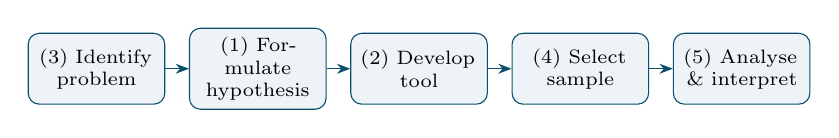
\begin{tikzpicture}[node distance=3mm,every node/.style={draw=brand,rounded corners,fill=soft,font=\scriptsize,align=center,text width=15mm,minimum height=9mm}]
\node (a) {(3) Identify problem}; \node[right=of a] (b) {(1) Formulate hypothesis}; \node[right=of b] (c) {(2) Develop tool}; \node[right=of c] (d) {(4) Select sample}; \node[right=of d] (e) {(5) Analyse \& interpret};
\foreach \x/\y in {a/b,b/c,c/d,d/e} \draw[-Stealth,brand] (\x)--(\y);
\end{tikzpicture}
\end{center}
The order is \textbf{3, 1, 2, 4, 5}.
\end{explain}
\end{question}

\begin{context}
\textbf{Directions for Q.~11 to 15:} Read the following passage and answer the questions.\par\smallskip
If the world is different today, we need to think, talk and engage accordingly. Falling back is unlikely to help, he said adding ``purposeful pursuit of national interest is shifting global dynamics''. Highlighting India's new approach in dealing with terrorism he compared ``lack of response to the terror attack of Mumbai in comparison to the way the country responded to the Uri and Pulwama strikes. On India walking away from the Regional Comprehensive Economic Partnership, the external affair minister said no agreement was better than having a bad agreement.

Giving a historical perspective to geopolitical issues, Jai-Shankar said ``For years India's position on the world state seemed assured but the 1962 conflict with China significantly damaged India's standing.
\end{context}
\begin{question}{11}
{RCEP stands for:\par}
\optsone{Regional Common Economic Party}{Regional Common Election Party}{Regional Comprehensive Election Partnership}{Regional Comprehensive Economic Partnership}
\answer{D}{Regional Comprehensive Economic Partnership}
\begin{explain}
\textbf{RCEP} is the \textbf{Regional Comprehensive Economic Partnership}, a free-trade agreement among the 10 ASEAN countries and China, Japan, South Korea, Australia and New Zealand (signed 2020). India withdrew from the negotiations in November 2019.
\end{explain}
\end{question}

\begin{question}{12}
{What was country's idea about Economic Partnership?\par}
\optsone{All Agreements are good}{Agreements are superior than country}{Nothing wrong in saying no to unfavourable agreement than having an awful agreement}{Say yes to all agreement}
\answer{C}{Nothing wrong in saying no to unfavourable agreement than having an awful agreement}
\begin{explain}
The minister said that ``\textbf{no agreement was better than having a bad agreement}''. Option (C) expresses this: there is nothing wrong in saying no to an unfavourable agreement rather than accepting an awful one.
\end{explain}
\end{question}

\begin{question}{13}
{The above statement was given by:\par}
\optstwo{Subhramanyam Swami}{Subhramanyam Jayshankar}{Ravi Shankar}{K. Subhramanyam}
\answer{B}{Subhramanyam Jayshankar}
\begin{explain}
The passage names \textbf{(S.) Jaishankar}, India's External Affairs Minister, as the speaker. Option (B) (``Subhramanyam Jayshankar'') refers to Dr.~Subrahmanyam Jaishankar.
\end{explain}
\end{question}

\begin{question}{14}
{India's New Approach on Terrorism is:\par}
\optsone{Wait till any action takes place}{Deny for any type of Action}{Earliest it was reactive, at present it is proactive}{Ready to loose for Peace}
\answer{C}{Earliest it was reactive, at present it is proactive}
\begin{explain}
The passage contrasts the ``lack of response'' to the 2008 Mumbai attack with India's response to the Uri (2016, surgical strikes) and Pulwama (2019, Balakot air strike) attacks. The approach has changed from \textbf{reactive to proactive}.
\end{explain}
\end{question}

\begin{question}{15}
{Year's back conflict of India with China was:\par}
\optstwo{National Issue}{International Issue}{Political Issue}{Geopolitical Issue}
\answer{D}{Geopolitical Issue}
\begin{explain}
The minister was ``giving a historical perspective to \textbf{geopolitical} issues'' when he spoke of the 1962 conflict with China, so the conflict is described as a geopolitical issue.
\end{explain}
\end{question}

\begin{question}{16}
{During the process of communication :\par}
\optsone{Sender encodes for the media and receiver decodes the message}{Sender decodes for the media and receiver encodes the message}{Medium encodes and decodes the message from sender}{Medium encodes and decodes the message from receiver}
\answer{A}{Sender encodes for the media and receiver decodes the message}
\begin{explain}
In the communication process the \textbf{sender encodes} the message into symbols suited to the medium, and the \textbf{receiver decodes} it to extract the meaning. The medium only carries the message.
\end{explain}
\end{question}

\begin{question}{17}
{Proxemics is the type of non-verbal communication which deals with:\par}
\optsfour{Appearance}{Touch}{Body organs}{Space}
\answer{D}{Space}
\begin{explain}
\textbf{Proxemics} deals with the use of \textbf{space} and distance in communication.
\why{Appearance belongs to artifactual communication; touch is haptics; movements of body organs are kinesics.}
\end{explain}
\end{question}

\begin{question}{18}
{Language barriers in communication exist due to :\par}
\optsone{the difference in the sender's recognition vocabulary and the receiver's user vocabulary}{the difference in sender's user vocabulary and the receiver's recognition vocabulary}{the sender's user vocabulary and the receiver's recognition vocabulary being alike}{the sender's recognition vocabulary and the receiver's user vocabulary being the same}
\answer{B}{the difference in sender's user vocabulary and the receiver's recognition vocabulary}
\begin{explain}
Every person has a larger \emph{recognition} vocabulary (words understood) than \emph{use} vocabulary (words actually used). A language barrier arises when the sender's \textbf{use vocabulary} contains words that are not in the receiver's \textbf{recognition vocabulary}, i.e.\ the two differ.
\end{explain}
\end{question}

\begin{question}{19}
{In intra-personal communication :\par}
\optsone{sender sends and receives the message}{sender sends and another receiver receives the message}{sender sends and two receivers receive the message}{sender sends and the group receives the message}
\answer{A}{sender sends and receives the message}
\begin{explain}
In \textbf{intrapersonal communication} a person communicates \emph{with oneself} (thinking, self-talk, reflection), so the same person is both sender and receiver.
\end{explain}
\end{question}

\begin{question}{20}
{The mass media impacts our society in different ways except:\par}
\optstwo{for influencing public opinion}{for modification of behaviour}{for changing values and belief system}{for judicial decisions}
\answer{D}{for judicial decisions}
\begin{explain}
Mass media shape public opinion, modify behaviour and change values and beliefs. \textbf{Judicial decisions} must be based on law and evidence and should not be influenced by the media, so this is the exception.
\end{explain}
\end{question}

\begin{question}{21}
{Find out the missing number: 4, 9, 20, 43, \ldots{}\par}
\optsfour{84}{96}{108}{133}
\dropped{}
\begin{explain}
The pattern is $\times2+1, \times2+2, \times2+3, \ldots$:
\[4\xrightarrow{\times2+1}9\xrightarrow{\times2+2}20\xrightarrow{\times2+3}43\xrightarrow{\times2+4}\mathbf{90}\]
90 is not among the options, so the agency \textbf{dropped} the question.
\end{explain}
\end{question}

\begin{question}{22}
{From Vadodara station, if we buy two tickets to station P and three tickets to station Q, the total cost is Rs. 77, but if we buy 3 tickets to station P and 5 tickets to station Q, the total cost is Rs. 124. The fare from Vadodara to P is:\par}
\optsfour{Rs. 13}{Rs. 14}{Rs. 18}{Rs. 20}
\answer{A}{Rs. 13}
\begin{explain}
$2P+3Q=77$ and $3P+5Q=124$.
Multiply the first equation by 5 and the second by 3: $10P+15Q=385$ and $9P+15Q=372$. Subtracting gives $P=\mathbf{13}$ (and $Q=17$).
Check: $2(13)+3(17)=77$ \checkmark; $3(13)+5(17)=124$ \checkmark.
\end{explain}
\end{question}

\begin{question}{23}
{300 gm of sugar solution has 40\% sugar in it. How much sugar should be added to make it 50\% in the solution ?\par}
\optsfour{30 gm}{40 gm}{50 gm}{60 gm}
\answer{D}{60 gm}
\begin{explain}
Sugar $=40\%\times300=120$ g. Let $x$ g of sugar be added.
\[\frac{120+x}{300+x}=\frac12\Rightarrow240+2x=300+x\Rightarrow x=\mathbf{60\ g}\]
\end{explain}
\end{question}

\begin{question}{24}
{Numbers in boxes given below follow the same arrangement. Find the missing numbers in the third box.\par}
\qfigure{\pyr{29}{16}{13}{27}{9}{33}\qquad\pyr{38}{21}{17}{35}{16}{43}\qquad\pyr{55}{30}{25}{?}{?}{?}}
\optsfour{65, 36, 63}{53, 24, 63}{49, 32, 53}{51, 25, 61}
\answer{D}{51, 25, 61}
\begin{explain}
Two rules hold in every box:
\begin{itemize}
\item \textbf{Bottom middle} $=$ (difference of the middle row)$^2$: $(16-13)^2=9$, $(21-17)^2=16$, so $(30-25)^2=\mathbf{25}$.
\item \textbf{Bottom left $+$ bottom right} $=2\times\text{top}+2$: $27+33=60=2(29)+2$, $35+43=78=2(38)+2$, so the sum must be $2(55)+2=112$. Also bottom right $-$ bottom left $=6, 8, \ldots$, so $\mathbf{10}$.
\end{itemize}
Left $+$ right $=112$ and right $-$ left $=10$ give \textbf{51 and 61}. The missing numbers are \textbf{51, 25, 61}.
\end{explain}
\end{question}

\begin{question}{25}
{By selling a mobile for Rs. 1,536, Amit lost 20\%. What percent shall he gain or loose by selling it for Rs. 2,000?\par}
\optstwo{A loss of 8.25\%}{A profit of 8.25\%}{A loss of 4.17\%}{A profit of 4.17\%}
\answer{D}{A profit of 4.17\%}
\begin{explain}
CP $=\dfrac{1536}{0.80}=1920$. New SP $=2000$, so profit $=80$.
\[\text{Profit \%}=\frac{80}{1920}\times100=\mathbf{4.17\%}\]
\end{explain}
\end{question}

\begin{question}{26}
{The Sanskrit word `Upamana' means:\par}
\optsfour{Implication}{Comparison}{Inference}{Perception}
\answer{B}{Comparison}
\begin{explain}
\textbf{Upamana} is knowledge by \textbf{comparison} or analogy. For example, a person told that ``a gavaya (wild ox) resembles a cow'' recognises a gavaya on seeing one.
\tip{Pratyaksha = perception; Anumana = inference; Upamana = comparison; Shabda = verbal testimony; Arthapatti = postulation; Anupalabdhi = non-perception.}
\end{explain}
\end{question}

\begin{question}{27}
{Odometer is to milage as compass is to:\par}
\optsfour{Speed}{Hiking}{Needle}{Direction}
\answer{D}{Direction}
\begin{explain}
An odometer is the instrument that measures \emph{mileage} (distance travelled); a compass is the instrument that shows \textbf{direction}. The relation is \emph{instrument : what it measures}.
\end{explain}
\end{question}

\begin{question}{28}
{Which of the following diagrams correctly represents Lions, Elephants and Animals?\par}
\optsfour{\tikz[baseline=-0.5ex,scale=0.3]{\draw (0,0) circle(1.3); \draw (-0.55,0) circle(0.5); \draw (0.55,0) circle(0.5);}}{\tikz[baseline=-0.5ex,scale=0.3]{\draw (0,0) circle(0.8); \draw (1.1,0) circle(0.8); \draw (2.2,0) circle(0.8);}}{\tikz[baseline=-0.5ex,scale=0.3]{\draw (0,0) circle(1.1); \draw (0,0.1) circle(0.5); \draw (1.6,0) circle(0.9);}}{\tikz[baseline=-0.5ex,scale=0.3]{\draw (0,0) circle(0.8); \draw (1.1,0) circle(0.8); \draw (3,0) circle(0.8);}}
\answer{A}{\tikz[baseline=-0.5ex,scale=0.3]{\draw (0,0) circle(1.3); \draw (-0.55,0) circle(0.5); \draw (0.55,0) circle(0.5);}}
\begin{explain}
Lions and elephants are both \textbf{animals}, and no lion is an elephant. So the two small circles must be \textbf{separate} and both lie \textbf{inside} the large ``Animals'' circle, as in diagram (A).
\begin{center}
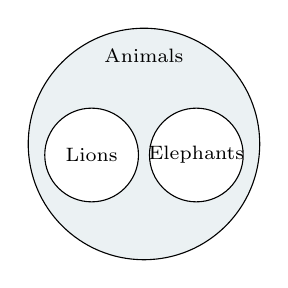
\begin{tikzpicture}[scale=0.7,font=\scriptsize]
\draw[fill=brand!8] (0,0) circle(2.1); \node at (0,1.6) {Animals};
\draw[fill=white] (-0.95,-0.2) circle(0.85) node {Lions}; \draw[fill=white] (0.95,-0.2) circle(0.85) node {Elephants};
\end{tikzpicture}
\end{center}
\end{explain}
\end{question}

\begin{question}{29}
{Nyaya Syllogism has \blank{} statement.\par}
\optsfour{One}{Five}{Three}{Two}
\answer{B}{Five}
\begin{explain}
The Nyaya syllogism (\emph{Panchavayava}) has \textbf{five} members: Pratijna (proposition), Hetu (reason), Udaharana (example), Upanaya (application) and Nigamana (conclusion).
\end{explain}
\end{question}

\begin{question}{30}
{Should high chimneys be installed in industries?\newline Arguments:\newline (I) Yes, it reduces pollution at ground level.\newline (II) No, it increases pollution in upper atmosphere.\par}
\optstwo{Only argument I is strong}{Only argument II is strong}{Either I or II is strong}{Both I and II are strong}
\answer{D}{Both I and II are strong}
\begin{explain}
Both arguments are \textbf{strong}. Tall chimneys disperse pollutants high up and so reduce ground-level concentration, which directly protects people (I). But they spread the pollution into the upper atmosphere and over larger areas, contributing to acid rain and similar problems (II). Each argument is important and directly related to the question.
\end{explain}
\end{question}

\begin{question}{31}
{The sum of squares of three numbers is 138, while sum of their products taken two at a time is 131. Their sum is:\par}
\optsfour{16}{20}{24}{26}
\answer{B}{20}
\begin{explain}
\[(a+b+c)^2=(a^2+b^2+c^2)+2(ab+bc+ca)=138+2(131)=400\ \Rightarrow\ a+b+c=\mathbf{20}\]
\end{explain}
\end{question}

\begin{question}{32}
{Given the following wage distributions:\par}
\qfigure{\begin{tabular}{lc}\toprule \textbf{Wages (Rs.)} & \textbf{No.\ of workers}\\\midrule
Less than 50 & 4\\ Less than 60 & 10\\ Less than 70 & 20\\ Less than 80 & 40\\ Less than 90 & 50\\\bottomrule\end{tabular}}
What percentage of workers earn wage more than Rs.~70?
\optsfour{50}{60}{65}{75}
\answer{B}{60}
\begin{explain}
This is a cumulative (``less than'') distribution. Total workers $=50$, and those earning less than Rs.~70 number 20.
Workers earning more than Rs.~70 $=50-20=30$, and $\dfrac{30}{50}\times100=\mathbf{60\%}$.
\end{explain}
\end{question}

\begin{question}{33}
{Study of the following graph carefully and answer the question:\par}
\qfigure{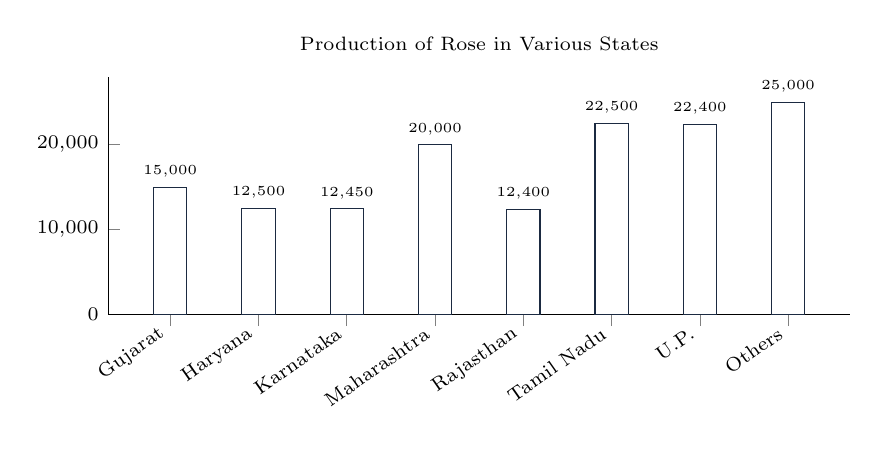
\begin{tikzpicture}
\begin{axis}[ybar,width=11cm,height=4.6cm,bar width=12pt,ymin=0,ymax=28000,
  symbolic x coords={Gujarat,Haryana,Karnataka,Maharashtra,Rajasthan,Tamil Nadu,U.P.,Others},xtick=data,
  x tick label style={rotate=35,anchor=east,font=\scriptsize},yticklabel style={font=\scriptsize},
  nodes near coords,every node near coord/.append style={font=\tiny},
  title={\scriptsize Production of Rose in Various States},axis x line*=bottom,axis y line*=left,
  scaled y ticks=false]
\addplot[fill=white,draw=ink] coordinates {(Gujarat,15000) (Haryana,12500) (Karnataka,12450) (Maharashtra,20000) (Rajasthan,12400) (Tamil Nadu,22500) (U.P.,22400) (Others,25000)};
\end{axis}
\end{tikzpicture}}
Which of the following state(s) contribute(s) less than 10 per cent in the total Rose production?
\optsone{Rajasthan and Karnataka}{Only Rajasthan}{Rajasthan, Karnataka, Harayana}{Rajasthan, Karnataka, Haryana and Gujarat}
\answer{C}{Rajasthan, Karnataka, Harayana}
\begin{explain}
Total $=15000+12500+12450+20000+12400+22500+22400+25000=142{,}250$, so 10\% $=14{,}225$.
States below 14,225: \textbf{Haryana} (12,500), \textbf{Karnataka} (12,450) and \textbf{Rajasthan} (12,400). Gujarat (15,000) is above 10\%.
\end{explain}
\end{question}

\begin{question}{34}
{Study the pie-chart carefully to answer the question:\par}
\qfigure{\begin{minipage}{0.45\linewidth}\centering
{\scriptsize\bfseries Percentage of students (Total 4500)}\\[2pt]
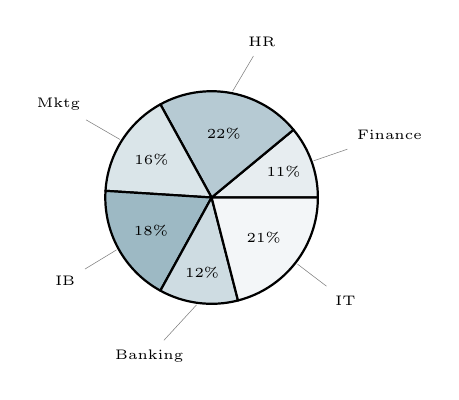
\begin{tikzpicture}\pie[radius=1.35,text=pin,font=\tiny,color={brand!10,brand!30,brand!15,brand!40,brand!20,brand!5}]{11/Finance,22/HR,16/Mktg,18/IB,12/Banking,21/IT}\end{tikzpicture}
\end{minipage}\hfill
\begin{minipage}{0.45\linewidth}\centering
{\scriptsize\bfseries Ratio of Men to Women}\\[2pt]\small
\begin{tabular}{lcc}\toprule Specialization & Men & Women\\\midrule
HR & 2 & 3\\ Marketing & 7 & 5\\ IB & 5 & 1\\ Banking & 17 & 10\\ IT & 1 & 2\\ Finance & 5 & 4\\\bottomrule\end{tabular}
\end{minipage}}
The number of women studying Finance is what percentage of the number of men studying the same?
\optsfour{70}{80}{85}{90}
\answer{B}{80}
\begin{explain}
Only the Finance ratio is needed: Men : Women $=5:4$.
\[\frac{\text{Women}}{\text{Men}}\times100=\frac45\times100=\mathbf{80\%}\]
(Numerically: Finance $=11\%$ of 4500 $=495$, of whom men $=275$ and women $=220$; $220/275=80\%$.)
\end{explain}
\end{question}

\begin{question}{35}
{The distribution of weights (in kg) of 50 students in a class is as follows:\par}
\qfigure{\begin{tabular}{cc}\toprule \textbf{Weight (kg)} & \textbf{No.\ of students}\\\midrule
35--38 & 3\\ 38--41 & 13\\ 41--44 & 19\\ 44--47 & 10\\ 47--50 & 5\\\bottomrule\end{tabular}}
What is the average weight of the class?
\optsfour{40.26}{41.88}{42.56}{43.25}
\answer{C}{42.56}
\begin{explain}
Use class mid-points $x$:
\begin{center}\small
\begin{tabular}{cccc}\toprule Class & $x$ & $f$ & $fx$\\\midrule
35--38 & 36.5 & 3 & 109.5\\ 38--41 & 39.5 & 13 & 513.5\\ 41--44 & 42.5 & 19 & 807.5\\ 44--47 & 45.5 & 10 & 455.0\\ 47--50 & 48.5 & 5 & 242.5\\\midrule
& & 50 & 2128.0\\\bottomrule\end{tabular}
\end{center}
Mean $=2128/50=\mathbf{42.56}$ kg.
\end{explain}
\end{question}

\begin{question}{36}
{`Internet Explorer' is a type of:\par}
\optstwo{Operating System}{Browser}{IP Address}{Compiler}
\answer{B}{Browser}
\begin{explain}
Internet Explorer (Microsoft, 1995--2022) is a \textbf{web browser}, software for accessing and viewing websites. Its successor is Microsoft Edge.
\end{explain}
\end{question}

\begin{question}{37}
{Which of the following is an open source software?\par}
\optstwo{Mozilla Firefox}{Acrobat Reader}{MS PowerPoint}{Windows}
\answer{A}{Mozilla Firefox}
\begin{explain}
\textbf{Mozilla Firefox} is free and open-source (released under the Mozilla Public License), so its source code is publicly available to study and modify.
\why{Acrobat Reader is freeware but proprietary; MS PowerPoint and Windows are proprietary commercial software.}
\end{explain}
\end{question}

\begin{question}{38}
{NMEICT stands for:\par}
\optsone{National Mission on Environment through ICT}{National Mission on English through ICT}{National Mission on Economics through ICT}{National Mission on Education through ICT}
\answer{D}{National Mission on Education through ICT}
\begin{explain}
\textbf{NMEICT} is the \textbf{National Mission on Education through Information and Communication Technology}, launched by MHRD in 2009. It supports e-content (e.g.\ NPTEL, e-PG Pathshala), connectivity and the SAKSHAT portal.
\end{explain}
\end{question}

\begin{question}{39}
{Dr. Ramesh is Assistant Professor in one college and wishes to do refresher course in his subject. Which of the following will be useful to him?\par}
\optsfour{ARPIT}{MOODLE}{NPTEL}{ePG Pathshala}
\answer{A}{ARPIT}
\begin{explain}
\textbf{ARPIT} (Annual Refresher Programme in Teaching), launched by MHRD in November 2018 on the SWAYAM platform, provides online refresher courses for higher-education faculty. Completing it counts for career advancement, like a conventional refresher course.
\why{MOODLE is an open-source LMS; NPTEL provides engineering and science courses; e-PG Pathshala provides PG e-content.}
\end{explain}
\end{question}

\begin{question}{40}
{Which of the following is not a social network?\par}
\optsfour{Linkedin}{Instagram}{Twitter}{ebay}
\answer{D}{ebay}
\begin{explain}
LinkedIn, Instagram and Twitter (X) are social-networking platforms. \textbf{eBay} is an \emph{e-commerce} (online auction and shopping) website.
\end{explain}
\end{question}

\begin{question}{41}
{Which steps are to be taken for abatement of air pollution?\newline (i) Use a CNG Car.\newline (ii) Stop the use of fire crackers during festivals.\newline (iii) Plant more number of trees.\newline (iv) Not to burn agricultural waste.\newline Choose the correct options:\par}
\optstwo{(iii) only}{(i), (iii) and (iv) only}{(i), (ii), (iii) and (iv)}{(i), (ii) and (iv) only}
\answer{C}{(i), (ii), (iii) and (iv)}
\begin{explain}
All four help abate air pollution: CNG vehicles emit fewer pollutants (i); avoiding firecrackers prevents spikes in particulate matter (ii); trees absorb pollutants and dust (iii); and not burning crop residue (stubble) prevents severe smog (iv). The answer is (i), (ii), (iii) and (iv).
\end{explain}
\end{question}

\begin{question}{42}
{Ozone depletion in the stratosphere causes:\par}
\optsone{increase in greenhouse effect}{cooling of the earth atmosphere system}{increase of infrared radiation in the troposphere}{increase of ultraviolet radiation in the troposphere}
\answer{D}{increase of ultraviolet radiation in the troposphere}
\begin{explain}
The stratospheric ozone layer absorbs most of the Sun's harmful UV-B radiation. When it is depleted, \textbf{more ultraviolet radiation reaches the troposphere} and the Earth's surface, causing skin cancer, cataracts and crop damage.
\end{explain}
\end{question}

\begin{question}{43}
{According to report of NITI Aayog, which city from South India will have zero ground water by 2020?\par}
\optstwo{Kozhikode}{Thiruvananthapuram}{Chennai}{Mysuru}
\answer{C}{Chennai}
\begin{explain}
NITI Aayog's \emph{Composite Water Management Index} report (2018) warned that 21 Indian cities, including Delhi, Bengaluru, \textbf{Chennai} and Hyderabad, could run out of groundwater by 2020. Among the options, Chennai is the South Indian city named. It faced an acute ``Day Zero'' water crisis in 2019.
\end{explain}
\end{question}

\begin{question}{44}
{The Air Quality Index (AQI) of one of the city is 190. It falls under which category?\par}
\optsfour{Very poor}{Poor}{Moderate}{Good}
\answer{C}{Moderate}
\begin{explain}
India's AQI bands: Good (0--50), Satisfactory (51--100), \textbf{Moderate (101--200)}, Poor (201--300), Very poor (301--400), Severe (401--500). An AQI of 190 is \textbf{Moderate}.
\end{explain}
\end{question}

\begin{question}{45}
{Which among the following is an environmental friendly polymer?\par}
\optstwo{Poly styrene}{Poly ethylene}{Poly lactic acid}{Poly propylene}
\answer{C}{Poly lactic acid}
\begin{explain}
\textbf{Poly lactic acid (PLA)} is made from renewable resources such as corn starch or sugarcane and is \textbf{biodegradable} and compostable, so it is environment-friendly.
\why{Polystyrene, polyethylene and polypropylene are petroleum-based, non-biodegradable plastics.}
\end{explain}
\end{question}

\begin{question}{46}
{The purpose of the National Assessment and Accreditation Council (NAAC) in India is \blank{}.\par}
\optstwo{Granting research funds}{Approving Academic Programs}{Quality Assurance}{Establishing Universities}
\answer{C}{Quality Assurance}
\begin{explain}
\textbf{NAAC} (est.~1994 by UGC, Bengaluru) assesses and accredits higher-education institutions, so its purpose is \textbf{quality assurance}.
\why{Grants are given by UGC/HEGC, programmes are approved by statutory councils and universities, and universities are established by legislatures.}
\end{explain}
\end{question}

\begin{question}{47}
{Which of the following organizations is responsible for Technical Education in India?\par}
\optsfour{AIU}{AICTE}{NCTE}{AIIMS}
\answer{B}{AICTE}
\begin{explain}
The \textbf{AICTE} (All India Council for Technical Education) is the statutory body for technical education: planning, standards, approvals and so on.
\why{AIU is the Association of Indian Universities; NCTE regulates teacher education; AIIMS is a medical institute.}
\end{explain}
\end{question}

\begin{question}{48}
{`IMPRINT' is a program that addresses \blank{}.\par}
\optsone{Major Science \& Engineering Challenges in India}{Major Agriculture Challenges}{Improvement of Academic Research}{Major Language and Literacy Challenges}
\answer{A}{Major Science \& Engineering Challenges in India}
\begin{explain}
\textbf{IMPRINT} (IMPacting Research INnovation and Technology), launched in 2015 by MHRD and led by the IITs and IISc, is a national initiative to address \textbf{major science and engineering challenges} in ten technology domains (health, energy, water, environment, security and others).
\end{explain}
\end{question}

\begin{question}{49}
{Which institution secured first rank in over all category of NIRF ranking 2019?\par}
\optstwo{IISc, Bangalore}{IIT, Madras}{IIT, Delhi}{IIT, Mumbai}
\answer{B}{IIT, Madras}
\begin{explain}
In \textbf{NIRF 2019} the \textbf{IIT Madras} ranked 1st in the Overall category, followed by IISc Bengaluru and IIT Delhi.
\end{explain}
\end{question}

\begin{question}{50}
{10+2+3 pattern of Education system in India was recommended by \blank{}.\par}
\optstwo{Kothari Commission}{Radhakrishnan Commission}{Balvantrai Mehta Committee}{Janardhan Reddy Committee}
\answer{A}{Kothari Commission}
\begin{explain}
The \textbf{Kothari Commission} (Education Commission, 1964--66) recommended a uniform \textbf{10+2+3} pattern of education, which the National Policy on Education 1968 adopted.
\why{The Radhakrishnan Commission (1948--49) dealt with university education; the Balwantrai Mehta Committee (1957) dealt with Panchayati Raj; the Janardhan Reddy Committee (1992) reviewed the NPE 1986.}
\end{explain}
\end{question}

\paperchapter{September 2018}{30 September 2018}{A}{50}{13th GSET}
\keytable{\kcell{1}{B} & \kcell{2}{A} & \kcell{3}{B} & \kcell{4}{C} & \kcell{5}{B} & \kcell{6}{B} & \kcell{7}{A} & \kcell{8}{D} & \kcell{9}{C} & \kcell{10}{B} \\
\kcell{11}{D} & \kcell{12}{B} & \kcell{13}{D} & \kcell{14}{C} & \kcell{15}{C} & \kcell{16}{A} & \kcell{17}{B} & \kcell{18}{C} & \kcell{19}{D} & \kcell{20}{B} \\
\kcell{21}{B} & \kcell{22}{A} & \kcell{23}{C} & \kcell{24}{B} & \kcell{25}{A} & \kcell{26}{A} & \kcell{27}{D} & \kcell{28}{C} & \kcell{29}{C} & \kcell{30}{D} \\
\kcell{31}{D} & \kcell{32}{C} & \kcell{33}{B} & \kcell{34}{B} & \kcell{35}{C} & \kcell{36}{C} & \kcell{37}{A} & \kcell{38}{C} & \kcell{39}{A} & \kcell{40}{D} \\
\kcell{41}{A} & \kcell{42}{C} & \kcell{43}{A} & \kcell{44}{B} & \kcell{45}{A} & \kcell{46}{C} & \kcell{47}{B} & \kcell{48}{C} & \kcell{49}{C} & \kcell{50}{D}}
\begin{question}{1}
{Name the philosopher who proposed the technique of questioning:\par}
\optsfour{John Dewey}{Socrates}{Comte}{Froebel}
\answer{B}{Socrates}
\begin{explain}
\textbf{Socrates} (469--399 BCE) taught by systematic questioning. The \emph{Socratic method} (maieutics, the ``midwife'' method) leads learners, through a chain of questions, to discover contradictions in their views and arrive at knowledge themselves.
\why{Dewey gave the problem/project method, Comte founded positivism, and Froebel founded the kindergarten (play-way method).}
\end{explain}
\end{question}

\begin{question}{2}
{Which of the following skills does not require high intellectual ability?\par}
\optstwo{Technical skills}{Mechanical skills}{Teaching skills}{Management skills}
\answer{A}{Technical skills}
\begin{explain}
According to the official key, \textbf{technical skills} (routine operational or procedural skills) require the least intellectual ability. Teaching and management skills demand high-level conceptual and interpersonal thinking.
\end{explain}
\end{question}

\begin{question}{3}
{Primary education in the mother tongue has been safeguarded in Article :\par}
\optsfour{29}{350}{220}{351}
\answer{B}{350}
\begin{explain}
\textbf{Article 350A} of the Constitution directs every State to provide adequate facilities for instruction in the \textbf{mother tongue at the primary stage} to children of linguistic minority groups.
\why{Article 29 protects the culture and language of minorities in general; Article 351 concerns the development of Hindi.}
\end{explain}
\end{question}

\begin{question}{4}
{What is the full form of CAI ?\par}
\optstwo{Computer Associated Instruction}{Computer Associated Information}{Computer Assisted Instruction}{Computer Assisted Information}
\answer{C}{Computer Assisted Instruction}
\begin{explain}
\textbf{CAI} is \textbf{Computer Assisted Instruction}: using computers to present instructional material, drill and practice, tutorials and simulations, with immediate feedback. It grew out of Skinner's programmed learning.
\end{explain}
\end{question}

\begin{question}{5}
{For maintaining discipline in the class:\par}
\optsone{Students should be severely punished for acts of indiscipline}{Teacher should try to make his teaching interesting}{Non-attending students should be turned out of the class}{Parents of the indisciplined students should be informed}
\answer{B}{Teacher should try to make his teaching interesting}
\begin{explain}
The best preventive discipline is \textbf{interesting, well-planned teaching}. When learners are engaged, indiscipline rarely arises.
\why{Severe punishment, expulsion from class or complaining to parents are negative measures that do not address the cause.}
\end{explain}
\end{question}

\begin{question}{6}
{If the sample drawn does not specify any condition about the parameter of the population, it is called :\par}
\optstwo{Selected statistics}{Distribution free statistics}{Parametric statistics}{Inferential statistics}
\answer{B}{Distribution free statistics}
\begin{explain}
Statistical tests that make \textbf{no assumptions about population parameters} (such as normality or equal variance) are called \textbf{non-parametric} or \textbf{distribution-free} statistics. Examples are chi-square, Mann--Whitney U, Wilcoxon, Kruskal--Wallis and Spearman's rho.
\end{explain}
\end{question}

\begin{question}{7}
{Validity of an experimental design refers to:\par}
\optsone{Maximise treatment variance and minimise error variance}{Minimise both treatment variance and error variance}{Testing the difference between treatment variance and error variance}{Minimise treatment variance and maximise error variance}
\answer{A}{Maximise treatment variance and minimise error variance}
\begin{explain}
Kerlinger's \textbf{MAX-MIN-CON} principle for a good experimental design: \textbf{MAX}imise systematic (treatment) variance, \textbf{MIN}imise error variance and \textbf{CON}trol extraneous variance. A design that does this yields valid conclusions.
\end{explain}
\end{question}

\begin{question}{8}
{Which one of the following is not considered as plagiarism?\par}
\optsone{Make use of the work of another and misrepresent it as your own}{Drawing content from the work of another without acknowledging the source}{Paraphrasing too closely to the original text}{Drawing content from another work and adapting it with due acknowledgement}
\answer{D}{Drawing content from another work and adapting it with due acknowledgement}
\begin{explain}
Using someone else's work \textbf{with proper acknowledgement} (citation) is legitimate scholarship, not plagiarism.
\why{Passing off others' work as one's own, using content without acknowledgement, and paraphrasing too closely are all forms of plagiarism.}
\end{explain}
\end{question}

\begin{question}{9}
{Bibliography refers to:\par}
\optsone{A true story written about someone}{A record of events presented in a report}{A list of sources used in a report and where they can be found}{List of abbreviations used in the report}
\answer{C}{A list of sources used in a report and where they can be found}
\begin{explain}
A \textbf{bibliography} is a list of all the \emph{sources} (books, articles, websites) consulted or cited, with enough detail (author, title, publisher, year, pages, URL) for readers to locate them.
\why{A true story about someone is a \emph{biography}; a list of abbreviations is a glossary or abbreviation list.}
\end{explain}
\end{question}

\begin{question}{10}
{Snowball sampling technique falls under the category of:\par}
\optstwo{Probability sampling}{Non-probability sampling}{Random sampling}{Quota sampling}
\answer{B}{Non-probability sampling}
\begin{explain}
\textbf{Snowball sampling} is a \textbf{non-probability} technique: existing participants recruit further participants from among their acquaintances. It is useful for hidden populations.
\end{explain}
\end{question}

\begin{context}
\textbf{Question Nos.~11--15 should be attempted from the following paragraph.} Below is given a passage followed by possible inferences which can be drawn from the facts stated in the passage. You have to examine each inference separately in the context of the passage and decide upon its degree of truth or falsity.\par\smallskip
\textbf{Passage:} ``The fifth conference of Labour Ministers of Non-Aligned and other developing countries which concluded in New Delhi on January 23, was not just another conference held under the auspices of International Labour Organization to discuss labour welfare. For one it was in the run-up to the world summit on social development that the conference was held, and for another, it was under the shadow of the demand by the industrialised countries to link labour standards to International trade through a social cause. The conference covered a large part of the agenda to be discussed at the summit to be held at Copenhagen in March, i.e.\ employment creation, poverty reduction and eradication and social integration.''
\end{context}
\begin{question}{11}
{The fourth conference of Labour Ministers was not held at New Delhi:\par}
\optstwo{The inference is probably true}{The inference is probably false}{The inference is definitely false}{The data are inadequate}
\answer{D}{The data are inadequate}
\begin{explain}
The passage tells us only where the \emph{fifth} conference was held (New Delhi). It says nothing about the venue of the fourth conference, so the \textbf{data are inadequate}.
\end{explain}
\end{question}

\begin{question}{12}
{blank{} organization took an active part in a conference of Labour Ministers for the first time.\par}
\optstwo{International Monetary Fund}{International Labour Organization}{World Health Organization}{UNICEF}
\answer{B}{International Labour Organization}
\begin{explain}
The conference was held ``under the auspices of the \textbf{International Labour Organization}''. The ILO is the organisation concerned with labour; the IMF, WHO and UNICEF are not mentioned. The key accepts (B).
\end{explain}
\end{question}

\begin{question}{13}
{Linking Labour standards to International trade would benefit the blank{} countries.\par}
\optsfour{Advanced}{Developing}{Developed}{Industrial}
\answer{D}{Industrial}
\begin{explain}
The demand to link labour standards to trade came from the \textbf{industrialised countries}. It would help them by making the products of low-wage developing countries less competitive, so the linkage would benefit the industrial countries.
\end{explain}
\end{question}

\begin{question}{14}
{Among the following topics which of them is \emph{not} discussed at the Copenhagen Conference?\par}
\optstwo{Employment}{Poverty}{Technology}{Social Integration}
\answer{C}{Technology}
\begin{explain}
The Copenhagen agenda was ``employment creation, poverty reduction and eradication and social integration''. \textbf{Technology} is not mentioned.
\end{explain}
\end{question}

\begin{question}{15}
{Which of the following is the reason for organizing the fifth conference of Labour Ministers?\par}
\optstwo{Compulsion by ILO}{To satisfy the government}{To run-up to the world summit}{Causal meeting of Ministers}
\answer{C}{To run-up to the world summit}
\begin{explain}
``\ldots it was \textbf{in the run-up to the world summit} on social development that the conference was held.''
\end{explain}
\end{question}

\begin{question}{16}
{Message is any signal that triggers the response of a\par}
\optsfour{Receiver}{Sender}{Channel}{Feedback}
\answer{A}{Receiver}
\begin{explain}
A message is any signal (verbal or non-verbal) sent by the source that stimulates a response in the \textbf{receiver}.
\end{explain}
\end{question}

\begin{question}{17}
{Our dress code is an example of \ldots{} communication.\par}
\optsfour{Verbal}{Non-verbal}{Written}{Spoken}
\answer{B}{Non-verbal}
\begin{explain}
Dress, appearance and personal artefacts communicate without words, so they are \textbf{non-verbal communication} (artifactics).
\end{explain}
\end{question}

\begin{question}{18}
{\ldots{} is the process by which the receiver interprets the symbols used by the source of the message.\par}
\optsfour{Listing}{Listening}{Decoding}{Encoding}
\answer{C}{Decoding}
\begin{explain}
\textbf{Decoding} is the receiver's interpretation of the symbols (words, signs, gestures) used by the sender, i.e.\ converting the message back into meaning.
\end{explain}
\end{question}

\begin{question}{19}
{Identify the correct sequence in the communication process:\par}
\optstwo{Sender - Channel - Message - Receiver}{Sender - Receiver - Message - Channel}{Sender - Receiver - Channel - Message}{Sender - Message - Channel - Receiver}
\answer{D}{Sender - Message - Channel - Receiver}
\begin{explain}
The communication process runs \textbf{Sender $\rightarrow$ Message $\rightarrow$ Channel $\rightarrow$ Receiver} (Berlo's SMCR model), with feedback returning to the sender.
\end{explain}
\end{question}

\begin{question}{20}
{The study of body language is called\par}
\optsfour{Proxemics}{Kinesics}{Phonetics}{Chronemics}
\answer{B}{Kinesics}
\begin{explain}
\textbf{Kinesics} (Ray Birdwhistell, 1952) is the study of body language: gestures, posture, facial expressions and eye movements.
\why{Proxemics = space; Phonetics = speech sounds; Chronemics = time.}
\end{explain}
\end{question}

\begin{question}{21}
{Find out missing number in the following:\par}
\qfigure{\petal{5}{3}{6}{8}{63}\quad\petal{2}{7}{3}{9}{41}\quad\petal{6}{7}{8}{5}{?}}
\optsfour{26}{82}{83}{86}
\answer{B}{82}
\begin{explain}
Centre $=$ (product of the top pair) $+$ (product of the bottom pair):
\[5\times3+6\times8=15+48=63,\qquad 2\times7+3\times9=14+27=41\]
\[6\times7+8\times5=42+40=\mathbf{82}\]
\end{explain}
\end{question}

\begin{question}{22}
{If P means x, R means +, T means $\div$ and S means -, then 18T3P9S8R6 = ?\par}
\optsfour{52}{2/3}{46}{58}
\answer{A}{52}
\begin{explain}
Replace the letters: $18\div3\times9-8+6$.
By BODMAS: $18\div3=6$; $6\times9=54$; $54-8+6=\mathbf{52}$.
\end{explain}
\end{question}

\begin{question}{23}
{Young is related to Old, in the same way Wide is related to\par}
\optsfour{Short}{Big}{Narrow}{Long}
\answer{C}{Narrow}
\begin{explain}
Young and old are \textbf{antonyms}; the antonym of wide is \textbf{narrow}.
\end{explain}
\end{question}

\begin{question}{24}
{If SUMMER is coded as RUNNER, the code for WINTER will be:\par}
\optsfour{SUITER}{VIOUER}{WALKER}{SUFFER}
\answer{B}{VIOUER}
\begin{explain}
SUMMER $\rightarrow$ RUNNER: S$\rightarrow$R ($-1$), U$\rightarrow$U, M$\rightarrow$N ($+1$), M$\rightarrow$N ($+1$), E$\rightarrow$E, R$\rightarrow$R.
Applying the same shifts to WINTER: W$-1=$V, I, N$+1=$O, T$+1=$U, E, R, giving \textbf{VIOUER}.
\end{explain}
\end{question}

\begin{question}{25}
{Find out the missing term in the following series : 0 7 26 63 124 \ldots{}\par}
\optsfour{215}{216}{248}{157}
\answer{A}{215}
\begin{explain}
Each term is $n^3-1$: $1-1=0$, $8-1=7$, $27-1=26$, $64-1=63$, $125-1=124$, so next $216-1=\mathbf{215}$.
\end{explain}
\end{question}

\begin{question}{26}
{In the following question choose the group of words that shows the same relationship as given at the top of the question : Play : Win : Lose\par}
\optstwo{Accident : Death : Survive}{Examination : Success : Determination}{Read : Book : Magazine}{Music : Dance : Art}
\answer{A}{Accident : Death : Survive}
\begin{explain}
Play has two opposite possible outcomes, win or lose. Likewise an \textbf{accident} may end in \textbf{death} or the victim may \textbf{survive}.
\why{In (B), determination is not an outcome of an examination; (C) and (D) are not outcome pairs.}
\end{explain}
\end{question}

\begin{question}{27}
{What is the missing number in the following sequence of numbers ? 84/14,12 81/18,9 88/?,11\par}
\optsfour{13}{14}{15}{16}
\answer{D}{16}
\begin{explain}
The number above each fraction is half the product of the two numbers below it:
\[\frac{14\times12}{2}=84,\qquad\frac{18\times9}{2}=81,\qquad\frac{?\times11}{2}=88\Rightarrow ?=\mathbf{16}\]
\end{explain}
\end{question}

\begin{question}{28}
{In a group of persons travelling in a bus, 6 persons can speak Malayalam, 15 can speak Hindi and 6 can speak Gujarati. In that group, none can speak any other language. If 2 persons in the group can speak two languages and one person can speak all the three languages, then how many persons are there in the group?\par}
\optsfour{21}{22}{23}{24}
\answer{C}{23}
\begin{explain}
Adding the language groups ($6+15+6=27$) counts a person who speaks exactly two languages twice and the person who speaks all three three times.
\[\text{Persons}=27-(\text{exactly two})-2(\text{all three})=27-2-2\times1=\mathbf{23}\]
\end{explain}
\end{question}

\begin{question}{29}
{In this question, two statements followed by four conclusions are given...\newline Statements:\newline (1) Some doors are mangoes.\newline (2) All mangoes are bananas.\newline Conclusions :\newline (I) All bananas are mangoes.\newline (II) All doors are bananas.\newline (III) Some doors are bananas.\newline (IV) Some mangoes are doors.\newline Which of the given conclusions logically follows...?\par}
\optstwo{Only I and II follows}{Only II and III follows}{Only III and IV follows}{Only II and IV follows}
\answer{C}{Only III and IV follows}
\begin{explain}
\begin{center}
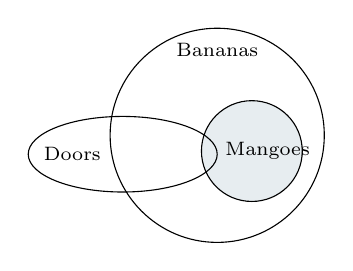
\begin{tikzpicture}[scale=0.8,font=\scriptsize]
\draw (0,0) circle(1.7); \node at (0,1.35){Bananas};
\draw[fill=brand!10] (0.55,-0.25) circle(0.8); \node at (0.8,-0.25){Mangoes};
\draw (-1.5,-0.3) ellipse(1.5 and 0.6); \node at (-2.3,-0.3){Doors};
\end{tikzpicture}
\end{center}
Some doors are mangoes, and all mangoes are bananas, so \textbf{some doors are bananas} (III follows). ``Some doors are mangoes'' converts to \textbf{some mangoes are doors} (IV follows). ``All bananas are mangoes'' (I) and ``All doors are bananas'' (II) do not follow. The answer is \textbf{only III and IV}.
\end{explain}
\end{question}

\begin{question}{30}
{The pie-diagram below shows various expenditures incurred in publishing a book:\par}
\qfigure{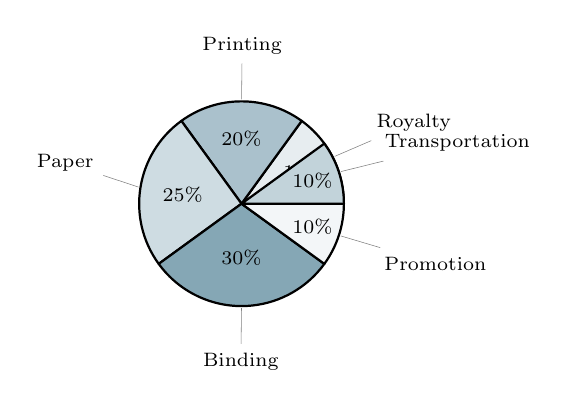
\begin{tikzpicture}\pie[radius=1.3,text=pin,font=\scriptsize,color={brand!10,brand!35,brand!20,brand!50,brand!5,brand!25}]{15/Royalty,20/Printing,25/Paper,30/Binding,10/Promotion,10/Transportation}\end{tikzpicture}}
If for an edition of the book, the cost of paper is Rs.~20,000, then what is the promotion cost for this edition?
\optsfour{Rs. 5,000}{Rs. 6,000}{Rs. 7,000}{Rs. 8,000}
\answer{D}{Rs. 8,000}
\begin{explain}
Paper $=25\%$ corresponds to Rs.~20,000, so $1\%=$ Rs.~800.
Promotion $=10\%=10\times800=$ \textbf{Rs.~8,000}.
\end{explain}
\end{question}

\begin{question}{31}
{If ${}^{2n}C_{n-1} : {}^{2n-1}C_{n} = 5:3$, then what is the value of $n$?\par}
\optsfour{2}{3}{4}{5}
\answer{D}{5}
\begin{explain}
\[\frac{{}^{2n}C_{n-1}}{{}^{2n-1}C_n}=\frac{\frac{(2n)!}{(n-1)!\,(n+1)!}}{\frac{(2n-1)!}{n!\,(n-1)!}}=\frac{2n\cdot n!}{(n+1)!}=\frac{2n}{n+1}\]
\[\frac{2n}{n+1}=\frac53\Rightarrow6n=5n+5\Rightarrow n=\mathbf{5}\]
\end{explain}
\end{question}

\begin{question}{32}
{The average of a set of 7 observations is 36 and that of another set of 13 observations is 46. What is the combined average of the set ?\par}
\optsfour{40.5}{41.5}{42.5}{43.5}
\answer{C}{42.5}
\begin{explain}
\[\bar x=\frac{7\times36+13\times46}{7+13}=\frac{252+598}{20}=\frac{850}{20}=\mathbf{42.5}\]
\end{explain}
\end{question}

\begin{question}{33}
{The following circuit operates only if there is a path of functional devices from left to right. The proportion that each device functions is shown on the graph. Assume that devices fail independently. What is the proportion that the circuit operates?\par}
\qfigure{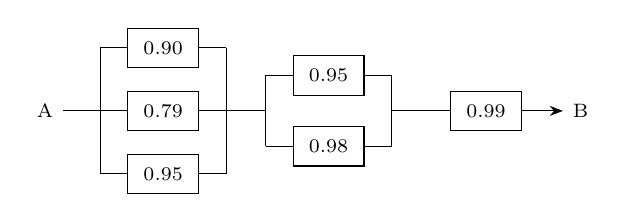
\begin{tikzpicture}[font=\scriptsize,box/.style={draw,minimum width=9mm,minimum height=5mm}]
\node (A) at (0,0) {A}; \node[box] (a) at (1.5,0.8) {0.90}; \node[box] (b) at (1.5,0) {0.79}; \node[box] (c) at (1.5,-0.8) {0.95};
\node[box] (d) at (3.6,0.45) {0.95}; \node[box] (e) at (3.6,-0.45) {0.98}; \node[box] (f) at (5.6,0) {0.99}; \node (B) at (6.8,0) {B};
\draw (A) -- (0.7,0); \draw (0.7,0.8) -- (0.7,-0.8); \foreach \n in {a,b,c} {\draw (0.7,0 |- \n.west) -- (\n.west); \draw (\n.east) -- (2.3,0 |- \n.east);}
\draw (2.3,0.8) -- (2.3,-0.8); \draw (2.3,0) -- (2.8,0); \draw (2.8,0.45) -- (2.8,-0.45);
\foreach \n in {d,e} {\draw (2.8,0 |- \n.west) -- (\n.west); \draw (\n.east) -- (4.4,0 |- \n.east);}
\draw (4.4,0.45) -- (4.4,-0.45); \draw (4.4,0) -- (f.west); \draw[-Stealth] (f.east) -- (B);
\end{tikzpicture}}
\optsfour{0.9725}{0.9879}{0.9915}{0.9998}
\answer{B}{0.9879}
\begin{explain}
A parallel block works unless \emph{all} its devices fail; blocks in series must \emph{all} work.
\[P_1=1-(0.10)(0.21)(0.05)=1-0.00105=0.99895\]
\[P_2=1-(0.05)(0.02)=0.999,\qquad P_3=0.99\]
\[P=0.99895\times0.999\times0.99\approx\mathbf{0.9879}\]
\end{explain}
\end{question}

\begin{question}{34}
{The value of $\dfrac{6^{2/3}\times\sqrt[3]{6^7}}{\sqrt[3]{6^6}}$ is:\par}
\optsfour{3}{6}{9}{12}
\answer{B}{6}
\begin{explain}
\[\frac{6^{2/3}\times6^{7/3}}{6^{6/3}}=6^{\frac23+\frac73-2}=6^{3-2}=\mathbf{6}\]
\end{explain}
\end{question}

\begin{question}{35}
{A bag contains 2 red, 3 green and 2 blue balls. Two balls are drawn at random. What is the probability that none of the balls drawn is blue ?\par}
\optsfour{$\dfrac27$}{$\dfrac{11}{21}$}{$\dfrac{10}{21}$}{$\dfrac57$}
\answer{C}{$\dfrac{10}{21}$}
\begin{explain}
Total balls $=7$, of which non-blue $=5$ (2 red $+$ 3 green).
\[P(\text{no blue})=\frac{{}^5C_2}{{}^7C_2}=\frac{10}{21}\]
\end{explain}
\end{question}

\begin{question}{36}
{CD-ROM stands for:\par}
\optstwo{Compactable Read Only Memory}{Compactable Data Read Only Memory}{Compact Disk Read Only Memory}{Common Disk Read Only Memory}
\answer{C}{Compact Disk Read Only Memory}
\begin{explain}
\textbf{CD-ROM} is \textbf{Compact Disc Read-Only Memory}, an optical disc holding about 700 MB that can be read but not rewritten.
\end{explain}
\end{question}

\begin{question}{37}
{WAN stands for:\par}
\optstwo{Wide Area Network}{Wireless Access Network}{Wireless Area Network}{Wide Access Network}
\answer{A}{Wide Area Network}
\begin{explain}
\textbf{WAN} is \textbf{Wide Area Network}, a network spanning large geographical areas (cities or countries). The Internet is the largest WAN.
\tip{PAN $<$ LAN $<$ MAN $<$ WAN, in increasing geographical coverage.}
\end{explain}
\end{question}

\begin{question}{38}
{A computer cannot 'boot', if it does not have the :\par}
\optstwo{Compiler}{Loader}{Operating System}{Keypad}
\answer{C}{Operating System}
\begin{explain}
\textbf{Booting} means loading the \textbf{operating system} into main memory when the computer starts (the BIOS/UEFI runs POST and then the boot loader). Without an OS the computer cannot boot.
\end{explain}
\end{question}

\begin{question}{39}
{Human beings are referred to as Homo sapiens. Which device is called Sillico sapiens ?\par}
\optsfour{Computer}{Hardware}{Robot}{Drone}
\answer{A}{Computer}
\begin{explain}
The \textbf{computer} is popularly called \emph{Silico sapiens}, a ``wise'' (thinking) machine built on silicon chips, just as humans are \emph{Homo sapiens}.
\end{explain}
\end{question}

\begin{question}{40}
{1 GB is equal to\par}
\optsfour{1250 megabytes}{1296 megabytes}{1150 megabytes}{1024 megabytes}
\answer{D}{1024 megabytes}
\begin{explain}
In the binary system, $1\ \text{GB}=2^{10}\ \text{MB}=\mathbf{1024\ MB}$.
\end{explain}
\end{question}

\begin{question}{41}
{Which is India's first bullet train project?\par}
\optstwo{Mumbai-Ahmedabad}{Delhi-Chandigarh}{Delhi-Jaipur}{Chennai-Kolkata}
\answer{A}{Mumbai-Ahmedabad}
\begin{explain}
India's first high-speed rail (bullet train) project is the \textbf{Mumbai--Ahmedabad High Speed Rail} corridor (about 508 km), built with Japanese Shinkansen technology. Its foundation stone was laid in September 2017.
\end{explain}
\end{question}

\begin{question}{42}
{Supreme Court of India has ordered the transition of vehicles to which BS level?\par}
\optsfour{BS-V}{BS-III}{BS-VI}{BS-IV}
\answer{C}{BS-VI}
\begin{explain}
In 2016 the Government decided to leapfrog from BS-IV directly to \textbf{BS-VI} emission norms. In October 2018 the Supreme Court ordered that no BS-IV vehicle be sold or registered from 1 April 2020, so the transition was to \textbf{BS-VI}.
\end{explain}
\end{question}

\begin{question}{43}
{Scientists have developed a new battery material based in \ldots{} with charging speed 5 times faster than lithium-ion batteries.\par}
\optsfour{Graphene}{Carbon}{Nitrate}{Chromium}
\answer{A}{Graphene}
\begin{explain}
Researchers (notably at the Samsung Advanced Institute of Technology) developed a \textbf{graphene}-based battery material (``graphene balls'') that allows charging about \textbf{five times faster} than conventional lithium-ion batteries.
\end{explain}
\end{question}

\begin{question}{44}
{Which is regarded as one of the world's hottest hotspots of biological diversity ?\par}
\optsfour{Rann of Kutch}{Western Ghats}{Eastern Ghats}{Thar Deserts}
\answer{B}{Western Ghats}
\begin{explain}
The \textbf{Western Ghats} (with Sri Lanka) form one of the world's 36 biodiversity hotspots and are regarded as one of the ``hottest'', with very high endemism. They are a UNESCO World Heritage Site (2012).
\tip{India's four hotspots: Himalaya, Indo-Burma, Western Ghats--Sri Lanka, and Sundaland (Nicobar Islands).}
\end{explain}
\end{question}

\begin{question}{45}
{Which Indian astrophysicist and Nobel laureate predicted rapidly rotating stars emitting polarised light ?\par}
\optstwo{S. Chandrasekhar}{C.V. Raman}{S. Ramanujam}{Venkat Raman Ramakrishnan}
\answer{A}{S. Chandrasekhar}
\begin{explain}
\textbf{S.~Chandrasekhar} (Nobel Prize in Physics, 1983) predicted that rapidly rotating stars would emit \textbf{polarised light}. Astronomers confirmed the prediction in 2017, about 70 years later, observing the star Regulus.
\end{explain}
\end{question}

\begin{question}{46}
{What is the full form of NIRF a methodology to rank higher education institutions in India?\par}
\optsone{National Institute of Research Framework}{National and International Ranking Framework}{National Institutional Ranking Framework}{National Inventory of Research Funding}
\answer{C}{National Institutional Ranking Framework}
\begin{explain}
\textbf{NIRF} is the \textbf{National Institutional Ranking Framework} (MHRD, 2015), which ranks HEIs on five parameters: TLR, RPP, GO, OI and Perception.
\end{explain}
\end{question}

\begin{question}{47}
{'SWAYAM' is a portal initiated by:\par}
\optstwo{NITI Aayog}{MHRD}{Ministry of I\&B}{Ministry of Railways}
\answer{B}{MHRD}
\begin{explain}
\textbf{SWAYAM} was initiated by the \textbf{Ministry of Human Resource Development (MHRD)}, now the Ministry of Education, and launched on 9 July 2017.
\end{explain}
\end{question}

\begin{question}{48}
{'AICTE' is responsible for the planning, coordination and management of:\par}
\optstwo{Teacher Education}{Distance Education}{Technical and Management Education}{School Education}
\answer{C}{Technical and Management Education}
\begin{explain}
The \textbf{AICTE} plans, coordinates and manages \textbf{technical and management education} (engineering, technology, management, pharmacy, architecture, hotel management and others).
\end{explain}
\end{question}

\begin{question}{49}
{In who's name the National Mission on Teachers and Teaching has been launched in India?\par}
\optstwo{Pt. Dindayal Upadhyaya}{Pt. Jawaharlal Nehru}{Pt. Madan Mohan Malaviya}{Pt. Ravishankar}
\answer{C}{Pt. Madan Mohan Malaviya}
\begin{explain}
The \textbf{Pandit Madan Mohan Malaviya National Mission on Teachers and Teaching (PMMMNMTT)} was launched in December 2014 to strengthen teacher education and faculty development at all levels.
\end{explain}
\end{question}

\begin{question}{50}
{In which state the first children's university was established in India?\par}
\optsfour{Maharashtra}{Rajasthan}{Madhya Pradesh}{Gujarat}
\answer{D}{Gujarat}
\begin{explain}
India's first \textbf{Children's University} was established at \textbf{Gandhinagar, Gujarat} in 2009 under the Children's University Act. It carries out research on child development and education.
\end{explain}
\end{question}

\paperchapter{August 2017}{27 August 2017}{A}{60}{GSET 2017}
\keytable{\kcell{1}{C} & \kcell{2}{A} & \kcell{3}{D} & \kcell{4}{D} & \kcell{5}{D} & \kcell{6}{C} & \kcell{7}{B} & \kcell{8}{B} & \kcell{9}{C} & \kcell{10}{B} \\
\kcell{11}{D} & \kcell{12}{B} & \kcell{13}{B} & \kcell{14}{C} & \kcell{15}{A} & \kcell{16}{C} & \kcell{17}{D} & \kcell{18}{B} & \kcell{19}{B} & \kcell{20}{D} \\
\kcell{21}{B} & \kcell{22}{B} & \kcell{23}{B} & \kcell{24}{B} & \kcell{25}{A} & \kcell{26}{B} & \kcell{27}{B} & \kcell{28}{A} & \kcell{29}{A} & \kcell{30}{D} \\
\kcell{31}{B} & \kcell{32}{A} & \kcell{33}{C} & \kcell{34}{D} & \kcell{35}{C} & \kcell{36}{B} & \kcell{37}{D} & \kcell{38}{B} & \kcell{39}{B} & \kcell{40}{A} \\
\kcell{41}{B} & \kcell{42}{B} & \kcell{43}{B} & \kcell{44}{D} & \kcell{45}{B} & \kcell{46}{C} & \kcell{47}{D} & \kcell{48}{D} & \kcell{49}{B} & \kcell{50}{B} \\
\kcell{51}{C} & \kcell{52}{D} & \kcell{53}{D} & \kcell{54}{B} & \kcell{55}{C} & \kcell{56}{A} & \kcell{57}{B} & \kcell{58}{B} & \kcell{59}{C} & \kcell{60}{C}}
\begin{question}{1}
{Education would be meaningful when it is \blank{} centric.\par}
\optsfour{Curriculum}{Society}{Student}{Teacher}
\answer{C}{Student}
\begin{explain}
Modern education is \textbf{child-centred (student-centred)}: the curriculum, methods and evaluation are organised around the learner's needs, interests, abilities and pace (Rousseau, Froebel, Dewey, Montessori). Education is meaningful only when it engages the learner actively.
\end{explain}
\end{question}

\begin{question}{2}
{The strength of project method lies in:\par}
\optstwo{Social participation}{Collection of information}{Teacher's instructions}{Individual engagement}
\answer{A}{Social participation}
\begin{explain}
In this paper the official key credits \textbf{social participation}. The project method, developed by W.~H.~Kilpatrick from Dewey's philosophy, has learners work together in groups on real-life, purposeful tasks. Learning thus takes place through cooperation and \emph{social participation}, in a lifelike social setting.
\tip{The same question in GSET Dec 2019 was keyed ``individualised engagement''. Both views are defensible, so always read the options carefully.}
\end{explain}
\end{question}

\begin{question}{3}
{Continuous and comprehensive and scholaristic evaluation means:\par}
\optsone{Scholaristic evaluation of students}{Physical evaluation of students}{Evaluation of students through continuous examination}{Evaluation of overall development of students through continuous evaluation}
\answer{D}{Evaluation of overall development of students through continuous evaluation}
\begin{explain}
\textbf{Continuous and Comprehensive Evaluation (CCE)} evaluates the \textbf{overall (scholastic and co-scholastic) development} of students \textbf{continuously} throughout the year. Continuous means regular formative and summative assessment. Comprehensive means covering cognitive, affective and psychomotor domains (academics, life skills, attitudes, co-curricular activities).
\end{explain}
\end{question}

\begin{question}{4}
{By using audio-visual teaching aids:\par}
\optsone{Students become active in classroom learning}{Teacher becomes active in teaching}{Teaching becomes effective}{All of the above}
\answer{D}{All of the above}
\begin{explain}
Audio-visual aids appeal to several senses at once. They make learners active participants, make the teacher's presentation more dynamic, and so make teaching more effective (``Seeing is believing''; Edgar Dale's Cone of Experience). All three statements are true.
\end{explain}
\end{question}

\begin{question}{5}
{Main objective of diagnostic test, is \blank{}\par}
\optsone{to know the content weakness of student}{to know the scholastic achievement of student}{to do remedial teaching}{(A) and (C) both}
\answer{D}{(A) and (C) both}
\begin{explain}
A \textbf{diagnostic test} pinpoints the specific \textbf{weaknesses or learning difficulties} of a student in the content, and its purpose is to plan \textbf{remedial teaching}. Hence (A) and (C) both.
\why{Measuring overall scholastic achievement is the job of an \emph{achievement} test.}
\end{explain}
\end{question}

\begin{question}{6}
{Who is a better teacher?\par}
\optsone{The one strictly following the disciplinary guidelines}{The one devoting full time to the school}{The one who is interested in overall development of students}{The one who develops quality leadership in his students}
\answer{C}{The one who is interested in overall development of students}
\begin{explain}
The best teacher is concerned with the \textbf{all-round (holistic) development} of students: intellectual, emotional, social, moral and physical. Strict discipline, long hours or leadership training alone are narrower goals.
\end{explain}
\end{question}

\begin{question}{7}
{`Placebo' effect means:\par}
\optstwo{Negative effect}{Positive effect}{Natural effect}{No effect}
\answer{B}{Positive effect}
\begin{explain}
A \textbf{placebo} is an inert treatment (e.g.\ a sugar pill). The \textbf{placebo effect} is the \emph{positive} improvement that occurs simply because the subject believes a treatment is being given. In experiments a placebo group controls for this expectation effect.
\tip{A negative effect produced by negative expectations is called the \emph{nocebo} effect.}
\end{explain}
\end{question}

\begin{question}{8}
{How many variables are there in the factorial research design of 2 $\times$ 3 $\times$ 2?\par}
\optsfour{two}{three}{seven}{twelve}
\answer{B}{three}
\begin{explain}
In a factorial design the notation $2\times3\times2$ gives one number \emph{per independent variable} (factor), each number being the number of levels of that factor. Three numbers mean \textbf{three} variables (with $2\times3\times2=12$ treatment combinations).
\end{explain}
\end{question}

\begin{question}{9}
{In the true experimental research design:\par}
\optsone{No control on external variables}{Less control on external variables}{Control on external variables by randomization}{No use of randomization}
\answer{C}{Control on external variables by randomization}
\begin{explain}
A \textbf{true experimental design} has three features: manipulation of the independent variable, a control group, and \textbf{random assignment} (randomisation), which controls extraneous (external) variables.
\end{explain}
\end{question}

\begin{question}{10}
{What is the full form of APA?\par}
\optstwo{American Philosophical Association}{American Psychological Association}{American Physics Association}{American Pharmacy Association}
\answer{B}{American Psychological Association}
\begin{explain}
\textbf{APA} is the \textbf{American Psychological Association}. Its \emph{Publication Manual} (7th ed., 2019) sets the ``APA style'' of referencing widely used in education and the social sciences.
\end{explain}
\end{question}

\begin{question}{11}
{During the process of data collection from the sample respondents, you obtained some sensitive information, what will be your ethical response in this regard?\par}
\optsone{Sharing the information with family members}{Sharing the information within colleagues}{Sharing the information with general public}{Keeping the information confidential}
\answer{D}{Keeping the information confidential}
\begin{explain}
Research ethics require \textbf{confidentiality}: information from respondents, especially sensitive information, must be kept private and used only for research purposes, with anonymity protected. Sharing it with family, colleagues or the public violates the informed-consent agreement.
\end{explain}
\end{question}

\begin{question}{12}
{In the historical research, external criticism means:\par}
\optstwo{content validity of documents}{validity of originality of documents}{to get information about documents}{to receive documents}
\answer{B}{validity of originality of documents}
\begin{explain}
In historical research, \textbf{external criticism} tests the \textbf{authenticity (genuineness or originality)} of a document or source: is it what it claims to be? (author, date, place, forgery). \textbf{Internal criticism} tests the \emph{credibility, accuracy and meaning of the content}.
\end{explain}
\end{question}

\begin{context}
\textbf{Read the following text and answer the questions 13 to 18.}\par\smallskip
The term `Street Children' is used to refer to children who live on the streets and are deprived of family care and protection. They live in abandoned buildings, containers, automobiles, parks or on street itself. A great deal has been written defining street children. The problem is that there are no precise categories but rather a continuum ranging from children who spend some time in the streets but basically live at home to those who live entirely in the streets and have no adult care. The street children live and work amidst trash, animals and open sewers. They are exposed to many diseases and are unlikely to receive any medical treatment as they cannot afford doctors or medicine. Other major problems of street children are: abuse, child labour, gender discrimination, homelessness and poverty. How can the civil society provide such children their basic constitutional right to health, freedom from violence and abuse is a big challenge.
\end{context}
\begin{question}{13}
{The nature of the above paragraph is:\par}
\optsfour{Analytical}{Descriptive}{Synthesis}{Consequential}
\answer{B}{Descriptive}
\begin{explain}
The paragraph \textbf{describes} who street children are, where they live and the problems they face. It does not analyse causes, synthesise views or trace consequences, so it is \textbf{descriptive}.
\end{explain}
\end{question}

\begin{question}{14}
{The term `Street Children' is a:\par}
\optstwo{Concept}{Definition}{Coined term}{Theoretical framework}
\answer{C}{Coined term}
\begin{explain}
The expression ``street children'' is a \textbf{coined term}: a phrase specially coined (by UNICEF and welfare agencies in the 1980s) to label children who live and work on the streets. The passage itself notes that ``a great deal has been written defining'' them, i.e.\ it is a label rather than a precise definition, concept or theoretical framework.
\end{explain}
\end{question}

\begin{question}{15}
{`Street Children' in this paragraph have been painted as children:\par}
\optstwo{Without home and without parents}{Working as child labourer}{Susceptible to diseases}{Devoid of their basic right}
\answer{A}{Without home and without parents}
\begin{explain}
The opening sentence paints street children as those ``who live on the streets and are deprived of family care and protection'', i.e.\ children \textbf{without home and without parents} (family). The other options (child labour, disease, lack of rights) are consequences mentioned later.
\end{explain}
\end{question}

\begin{question}{16}
{`Street Children' are exposed to many diseases because:\par}
\optstwo{They do not have home}{They have no adult care}{They live near open sewer}{They are discriminated}
\answer{C}{They live near open sewer}
\begin{explain}
According to the official key the main reason is that they \textbf{have no adult care}. With no one to look after them, they live amid trash and sewers and cannot get medical treatment.
\end{explain}
\end{question}

\begin{question}{17}
{Choose the correct answer -- Street children:\par}
\optsone{Live secured life}{They are poor but get care from society}{Get free medical treatment}{Deprived from family care}
\answer{D}{Deprived from family care}
\begin{explain}
Street children are ``\textbf{deprived of family care} and protection'' (first sentence). The other options contradict the passage.
\end{explain}
\end{question}

\begin{question}{18}
{Which one given below is not correct for street children?\par}
\optstwo{They live in abandoned buildings}{They get medical treatment}{They do not get any care}{They are exposed to many diseases}
\answer{B}{They get medical treatment}
\begin{explain}
The passage says they ``are unlikely to receive any medical treatment''. So ``they get medical treatment'' is \textbf{not correct}.
\end{explain}
\end{question}

\begin{question}{19}
{In communication, attributing our own thoughts and feelings to others is called \blank{}\par}
\optsfour{Stereotyping}{Projection}{Halo effect}{Barrier}
\answer{B}{Projection}
\begin{explain}
\textbf{Projection} is the perceptual tendency to attribute one's own thoughts, feelings or motives to others.
\why{Stereotyping judges a person by the group they belong to; the halo effect lets one good trait colour the overall impression.}
\end{explain}
\end{question}

\begin{question}{20}
{Rearrange the steps in order in the process of interpersonal communication:\newline (1) Sender\newline (2) Receiver\newline (3) Message\newline (4) Feedback\newline (5) Channel\newline (6) Encoding\par}
\optsfour{123456}{134265}{132146}{163524}
\answer{D}{163524}
\begin{explain}
The interpersonal communication process in order:
\begin{center}
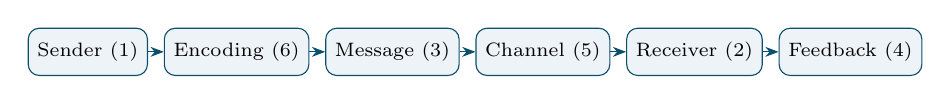
\begin{tikzpicture}[node distance=2mm,every node/.style={draw=brand,rounded corners,fill=soft,font=\scriptsize,minimum height=6mm}]
\node (a) {Sender (1)}; \node[right=of a] (b) {Encoding (6)}; \node[right=of b] (c) {Message (3)}; \node[right=of c] (d) {Channel (5)}; \node[right=of d] (e) {Receiver (2)}; \node[right=of e] (f) {Feedback (4)};
\foreach \x/\y in {a/b,b/c,c/d,d/e,e/f} \draw[-Stealth,brand] (\x)--(\y);
\end{tikzpicture}
\end{center}
The order is \textbf{1-6-3-5-2-4}, i.e.\ 163524.
\end{explain}
\end{question}

\begin{question}{21}
{The content of communication is called \blank{}\par}
\optsfour{noise}{message}{channel}{distortion}
\answer{B}{message}
\begin{explain}
The \textbf{message} is the content of communication: the information, idea or feeling that the sender wants to convey.
\end{explain}
\end{question}

\begin{question}{22}
{The process by which the receiver interprets the symbols used by the source of message by converting them into concept and ideas is called \blank{}\par}
\optsfour{Encoding}{Decoding}{Listening}{Speaking}
\answer{B}{Decoding}
\begin{explain}
\textbf{Decoding}: the receiver interprets the symbols and converts them back into concepts and ideas.
\end{explain}
\end{question}

\begin{question}{23}
{The main purpose of communication is to impart \blank{}\par}
\optsfour{Training}{Information}{Discipline}{Skill}
\answer{B}{Information}
\begin{explain}
The primary purpose of communication is to impart (share) \textbf{information}. Training, discipline and skills are specific outcomes that depend on communicating information.
\end{explain}
\end{question}

\begin{question}{24}
{Which of the following is the most effective way of communication?\par}
\optstwo{Verbal communication}{Written communication}{Non-verbal communication}{Silence}
\answer{B}{Written communication}
\begin{explain}
The official key gives \textbf{written communication}: it is precise, permanent, verifiable, can reach many people and can be referred to repeatedly, which makes it the most reliable and effective form, especially in formal settings.
\end{explain}
\end{question}

\begin{question}{25}
{Find out the next term in the following series:\newline 0, 3, 8, 15, 24, \ldots{}\par}
\optsfour{35}{32}{39}{37}
\answer{A}{35}
\begin{explain}
Each term is $n^2-1$: $1-1=0$, $4-1=3$, $9-1=8$, $16-1=15$, $25-1=24$, so next $36-1=\mathbf{35}$. (Differences: 3, 5, 7, 9, 11.)
\end{explain}
\end{question}

\begin{question}{26}
{Find the missing number in the following:\par}
\qfigure{\begin{tabular}{|c|c|c|}\hline 0 & 2 & 4\\\hline 1 & 3 & 5\\\hline 7 & 9 & 11\\\hline 0 & 24 & ?\\\hline\end{tabular}}
\optsfour{20}{64}{59}{29}
\answer{B}{64}
\begin{explain}
Work column by column: bottom $=$ top $\times$ (sum of the two middle numbers).
\[0\times(1+7)=0,\qquad 2\times(3+9)=24,\qquad 4\times(5+11)=\mathbf{64}\]
\end{explain}
\end{question}

\begin{question}{27}
{If HEALTH is written as GSKZDG, then how will NORTH be written in that code?\par}
\optsfour{OPSUI}{GSQNM}{FRPML}{IUSPO}
\answer{B}{GSQNM}
\begin{explain}
HEALTH $\rightarrow$ GSKZDG: \emph{reverse} the word (HTLAEH) and then move each letter \emph{one step back}: H$\rightarrow$G, T$\rightarrow$S, L$\rightarrow$K, A$\rightarrow$Z, E$\rightarrow$D, H$\rightarrow$G.
NORTH reversed is HTRON; one step back gives \textbf{GSQNM}.
\end{explain}
\end{question}

\begin{question}{28}
{If L stands for (+), M stands for (--), N stands for ($\times$) and P stands for ($\div$), then 14N 10L 42P 2M 8 = ?\par}
\optsfour{153}{216}{248}{251}
\answer{A}{153}
\begin{explain}
Substituting: $14\times10+42\div2-8=140+21-8=\mathbf{153}$.
\end{explain}
\end{question}

\begin{question}{29}
{A person's age is 3 times more than the age of his friend. The total of their ages is 64 years. Find the ages of the person and his friend:\par}
\optsfour{48, 16}{16, 64}{64, 16}{22, 42}
\answer{A}{48, 16}
\begin{explain}
The key reads ``3 times more than'' as ``3 times''. Friend $=x$, person $=3x$, $4x=64\Rightarrow x=16$. The ages are \textbf{48 and 16}.
\end{explain}
\end{question}

\begin{question}{30}
{If (A + B) > (C + D) and (B + C) > (A + D), then it is definite that:\par}
\optsfour{D > B}{C > D}{A > D}{B > D}
\answer{D}{B > D}
\begin{explain}
Add the two inequalities:
\[(A+B)+(B+C)>(C+D)+(A+D)\ \Rightarrow\ A+2B+C>A+C+2D\ \Rightarrow\ B>D\]
So \textbf{B $>$ D} is definite.
\end{explain}
\end{question}

\begin{question}{31}
{In the following question there is a certain relationship between two given words of one side of :: and one word on the other side of it, choose the correct alternative:\newline Aryabhatta : Mathematician :: Varahmihira : ?\par}
\optsfour{Physician}{Astronomer}{Scientist}{Architect}
\answer{B}{Astronomer}
\begin{explain}
Aryabhata was a mathematician (and astronomer); \textbf{Varahamihira} (6th century, \emph{Pancha-Siddhantika}, \emph{Brihat-Samhita}) is best known as an \textbf{astronomer} and astrologer.
\end{explain}
\end{question}

\begin{question}{32}
{Study the diagram below and identify the region representing youth who are employed but not educated:\par}
\qfigure{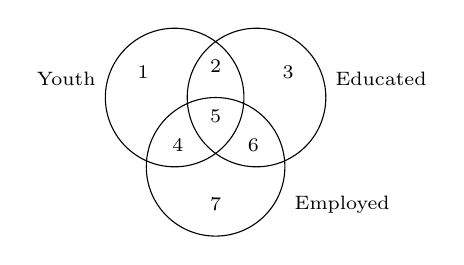
\begin{tikzpicture}[scale=0.8,font=\scriptsize]
\draw (0,0.5) circle(1.1); \draw (1.3,0.5) circle(1.1); \draw (0.65,-0.6) circle(1.1);
\node at (-0.5,0.9){1}; \node at (0.65,1.0){2}; \node at (1.8,0.9){3}; \node at (0.05,-0.25){4}; \node at (0.65,0.2){5}; \node at (1.25,-0.25){6}; \node at (0.65,-1.2){7};
\node[left] at (-1.1,0.8){Youth}; \node[right] at (2.4,0.8){Educated}; \node[right] at (1.75,-1.2){Employed};
\end{tikzpicture}}
\optsfour{4 only}{5, 6}{1, 4, 7}{4, 7}
\answer{A}{4 only}
\begin{explain}
The required region is \emph{inside} Youth, \emph{inside} Employed and \emph{outside} Educated. Only region \textbf{4} satisfies all three conditions.
\why{5 is also educated, 6 is not youth, and 7 is employed only (not youth).}
\end{explain}
\end{question}

\begin{question}{33}
{The question below consists of two statements numbered I and II. You have to decide whether the data provided in the statements are sufficient to answer the question.\\
\textbf{How is Tanya related to the man in the photograph?}\\
(I) Man in the photograph is the only son of Tanya's grandfather.\\
(II) The man in photograph has no brothers or sisters and his father is Tanya's grandfather.\par}
\optsone{Statement I alone is sufficient, II is not}{Statement II alone is sufficient, I is not}{Either statement I or II alone is sufficient}{Both statements together are not sufficient}
\answer{C}{Either statement I or II alone is sufficient}
\begin{explain}
The official key holds that each statement alone establishes that the man is the only son of Tanya's grandfather, and therefore \textbf{Tanya's father}. (Strictly, Tanya could also be a daughter's child; the setters assume the paternal line.) Both statements give the same information, so \textbf{either I or II} alone suffices.
\end{explain}
\end{question}

\begin{question}{34}
{How many triangles are there in the following figure?\par}
\qfigure{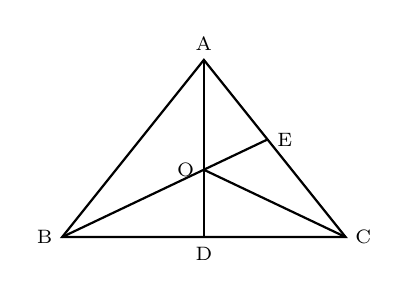
\begin{tikzpicture}[scale=0.9,font=\scriptsize]
\coordinate (A) at (0,2.5); \coordinate (B) at (-2,0); \coordinate (C) at (2,0); \coordinate (D) at (0,0);
\coordinate (O) at (0,0.95); \coordinate (E) at ($(A)!0.449!(C)$);
\draw[thick] (A)--(B)--(C)--cycle; \draw[thick] (A)--(D); \draw[thick] (B)--(E); \draw[thick] (C)--(O);
\foreach \p/\pos in {A/above,B/left,C/right,D/below,O/left,E/right} \node[\pos] at (\p) {\p};
\end{tikzpicture}}
\optsfour{6}{10}{11}{12}
\answer{D}{12}
\begin{explain}
Label the points as in the figure. The lines are AB, AC (through E), BC (through D), AD (through O), BE (through O) and CO. The triangles are:
\begin{center}\small
ABD, ABO, ABC, ABE, ADC, AOC, AOE, BOD, BOC, BEC, ODC, OEC
\end{center}
Total $=$ \textbf{12}.
\end{explain}
\end{question}

\begin{question}{35}
{In the following question, four words have been given, out of which three are alike in some manner and the fourth one is different. Choose the odd one.\par}
\optsfour{Veena}{Sitar}{Drum}{Guitar}
\answer{C}{Drum}
\begin{explain}
Veena, sitar and guitar are \textbf{string} instruments; the \textbf{drum} is a percussion instrument, so it is the odd one out.
\end{explain}
\end{question}

\begin{question}{36}
{In the question below, there are two statements labelled as Assertion (A) and Reason (R).\\
\textbf{Assertion (A):} Indian President is the head of country.\\
\textbf{Reason (R):} Indian Parliament consists of the President, Lok Sabha and Rajya Sabha.\par}
\optsone{If both (A) and (R) are true and (R) is the correct explanation of (A)}{Both (A) and (R) are true but (R) is not the correct explanation of (A)}{(A) is true (R) is false}{(A) is false (R) is true}
\answer{B}{Both (A) and (R) are true but (R) is not the correct explanation of (A)}
\begin{explain}
Both statements are true. The President is the constitutional Head of State (Art.~52--53), and Parliament consists of the President and the two Houses (Art.~79). But being part of Parliament is not \emph{why} the President is head of the country, so R does not explain A.
\end{explain}
\end{question}

\begin{question}{37}
{The bar graph given below shows the percentage distribution of total expenditure of a company under various expense heads during 2015. Study the graph and answer the questions that follows:\par}
\qfigure{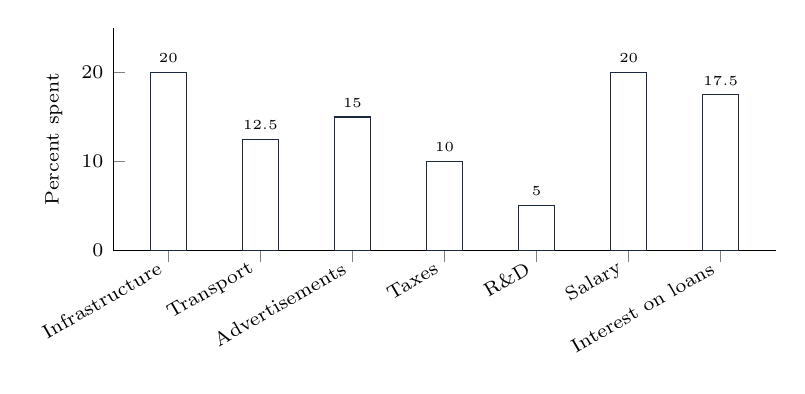
\begin{tikzpicture}
\begin{axis}[ybar,width=10cm,height=4.4cm,bar width=13pt,ymin=0,ymax=25,
  symbolic x coords={Infrastructure,Transport,Advertisements,Taxes,R\&D,Salary,Interest on loans},xtick=data,
  x tick label style={rotate=30,anchor=east,font=\scriptsize},yticklabel style={font=\scriptsize},
  nodes near coords,every node near coord/.append style={font=\tiny},ylabel={\scriptsize Percent spent},
  axis x line*=bottom,axis y line*=left]
\addplot[fill=white,draw=ink] coordinates {(Infrastructure,20) (Transport,12.5) (Advertisements,15) (Taxes,10) (R\&D,5) (Salary,20) (Interest on loans,17.5)};
\end{axis}
\end{tikzpicture}}
The expenditures on the interests on loans is by what percentage more than the expenditures on transport?
\optsfour{10\%}{20\%}{30\%}{40\%}
\answer{D}{40\%}
\begin{explain}
Interest on loans $=17.5\%$; transport $=12.5\%$.
\[\frac{17.5-12.5}{12.5}\times100=\frac{5}{12.5}\times100=\mathbf{40\%}\]
\end{explain}
\end{question}

\begin{question}{38}
{The following pie-chart shows the sources of funds to be collected by the National Highways Authority of India (NHAI) for its phase-II projects. Study the pie-chart and answer the question that follow:\par}
\qfigure{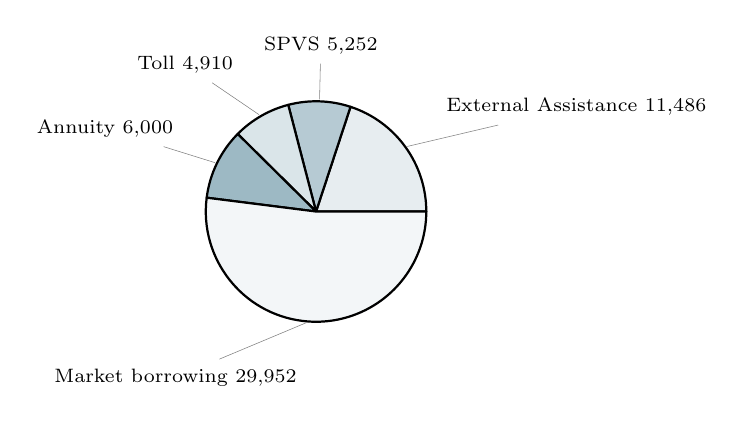
\begin{tikzpicture}\pie[radius=1.4,text=pin,hide number,font=\scriptsize,color={brand!10,brand!30,brand!15,brand!40,brand!5}]{19.94/External Assistance 11{,}486,9.12/SPVS 5{,}252,8.52/Toll 4{,}910,10.42/Annuity 6{,}000,52/Market borrowing 29{,}952}\end{tikzpicture}}
Total funds to be arranged for projects (phase II) $=$ Rs.~57,600 crores. The approximate ratio of funds to be arranged through toll and that through market borrowing is:
\optsfour{2 : 9}{1 : 6}{3 : 11}{2 : 5}
\answer{B}{1 : 6}
\begin{explain}
\[\frac{\text{Toll}}{\text{Market borrowing}}=\frac{4910}{29952}\approx\frac{1}{6.1}\approx\mathbf{1:6}\]
\end{explain}
\end{question}

\begin{question}{39}
{A researcher wants to study the association between gender and using a mobile phone. Data collected for this study will be \blank{}\par}
\optstwo{Quantitative data}{Qualitative data}{Continuous data}{Classified data}
\answer{B}{Qualitative data}
\begin{explain}
Gender (male/female) and mobile-phone use (user/non-user) are \textbf{categorical attributes}, i.e.\ qualities rather than measured quantities. The data are therefore \textbf{qualitative (nominal)}, typically analysed with a chi-square test of association.
\end{explain}
\end{question}

\begin{question}{40}
{A Government agency responsible for collection of various types of data in India is CSO. What is its full form?\par}
\optstwo{Central Statistical Office}{Central Statistical Organisation}{Central State Organisation}{Central Staff Organisation}
\answer{A}{Central Statistical Office}
\begin{explain}
\textbf{CSO} was the \textbf{Central Statistics Office} under the Ministry of Statistics and Programme Implementation (MoSPI), and the key's ``Central Statistical Office'' is this body. It compiled national accounts, GDP, IIP, CPI and so on. In 2019 it merged with the NSSO to form the \emph{National Statistical Office (NSO)}.
\end{explain}
\end{question}

\begin{question}{41}
{In order to show the strengths of PG and Ph.D. students in TEN different institutions of a state, most suitable diagram will be:\par}
\optstwo{Pie chart}{Two pie charts}{Multiple bar diagram}{Two Multiple bar diagrams}
\answer{B}{Two pie charts}
\begin{explain}
The official key gives \textbf{two pie charts}. Each chart shows how one category, PG students in one and PhD students in the other, is distributed among the ten institutions, i.e.\ each institution's share. (A multiple-bar diagram would be the choice for comparing absolute numbers side by side.)
\end{explain}
\end{question}

\begin{question}{42}
{The following table gives the percentage distribution of five states: P, Q, R, S and T on the basis of poverty line and also on the basis of gender. Study the table and answer the question:\par}
\qfigure{\small
\begin{tabular}{c c cc}\toprule
& & \multicolumn{2}{c}{\textbf{Males : Females}}\\\cmidrule(l){3-4}
\textbf{State} & \textbf{\% below poverty line} & \textbf{Below PL} & \textbf{Above PL}\\\midrule
P & 35 & 5 : 6 & 6 : 7\\ Q & 25 & 3 : 5 & 4 : 5\\ R & 24 & 1 : 2 & 2 : 3\\ S & 19 & 3 : 2 & 4 : 3\\ T & 15 & 5 : 3 & 3 : 2\\\bottomrule
\end{tabular}}
What will be the number of females above poverty line in the state S if it is known that population of state S is 7 million?
\optsfour{3 million}{2.43 million}{1.33 million}{5.7 million}
\answer{B}{2.43 million}
\begin{explain}
State S: above poverty line $=100-19=81\%$ of 7 million $=5.67$ million.
Females : males above PL $=3:(4+3)$, so females $=\tfrac37\times5.67=\textbf{2.43 million}$.
\end{explain}
\end{question}

\begin{question}{43}
{Created by Kevin Systrome and Mike Kriger, this app was acquired by facebook in April 2012, what it is?\par}
\optsfour{Twitter}{Instagram}{Whatsapp}{Linkedin}
\answer{B}{Instagram}
\begin{explain}
\textbf{Instagram} was created by Kevin Systrom and Mike Krieger (launched October 2010) and acquired by Facebook in April 2012 for about US\$1 billion.
\end{explain}
\end{question}

\begin{question}{44}
{`NPTEL' a project funded by MHRD, Govt. of India represents \blank{}\par}
\optsone{National Productivity Technique of Educational Leadership}{National Programme of Telephone Emergency Locator}{North Province Teacher Education Library}{National Programme on Technology Enhanced Learning}
\answer{D}{National Programme on Technology Enhanced Learning}
\begin{explain}
\textbf{NPTEL} is the \textbf{National Programme on Technology Enhanced Learning}, a joint initiative of the IITs and IISc funded by MHRD (since 2003). It offers online courses in engineering and science and is a SWAYAM national coordinator.
\end{explain}
\end{question}

\begin{question}{45}
{URL provides a standard hierarchical way of identifying and locating internet resources on World Wide Web (www). What does URL stand for?\par}
\optstwo{Uniform Recurrence Locator}{Uniform Resource Locator}{Uniform Remote Locator}{Uniform Revised Locator}
\answer{B}{Uniform Resource Locator}
\begin{explain}
\textbf{URL} is \textbf{Uniform Resource Locator}, the web address of a resource, e.g.\ \texttt{https://www.example.com/index.html} (protocol, domain, path).
\end{explain}
\end{question}

\begin{question}{46}
{It is a unique numeric identifier used to specify a particular host computer on a particular network, what it is?\par}
\optsfour{LP address}{UP address}{IP address}{IL address}
\answer{C}{IP address}
\begin{explain}
An \textbf{IP (Internet Protocol) address} is the unique numerical label assigned to each device on a network. IPv4 addresses are 32-bit (e.g.\ 192.168.1.1); IPv6 addresses are 128-bit.
\end{explain}
\end{question}

\begin{question}{47}
{This symbol was introduced by Ray Tomlinson in 1971. What it is?\par}
\optsfour{!}{\%}{\$}{@}
\answer{D}{@}
\begin{explain}
\textbf{Ray Tomlinson} sent the first network e-mail on ARPANET in 1971 and chose the \textbf{``@''} symbol to separate the user name from the host name.
\end{explain}
\end{question}

\begin{question}{48}
{HTML stands for:\par}
\optstwo{High text markup language}{Hypertext marketing language}{Hypertext makeup language}{Hypertext markup language}
\answer{D}{Hypertext markup language}
\begin{explain}
\textbf{HTML} is \textbf{HyperText Markup Language}, the standard language for creating web pages, devised by Tim Berners-Lee (1991).
\end{explain}
\end{question}

\begin{question}{49}
{Which plant is used in biodiesel?\par}
\optsfour{Palm tree}{Jatropha}{Coconut tree}{Eucalyptus}
\answer{B}{Jatropha}
\begin{explain}
\textbf{Jatropha curcas} is the main non-edible oilseed plant promoted for biodiesel in India (National Mission on Biodiesel, 2003). It grows on wasteland and does not compete with food crops.
\end{explain}
\end{question}

\begin{question}{50}
{Global environmental problem is mainly due to:\par}
\optstwo{Climate change}{Increasing population}{Rising temperature}{Melting of Iceberg}
\answer{B}{Increasing population}
\begin{explain}
The official key gives \textbf{increasing population}. A growing population drives higher consumption of resources, pollution, deforestation and emissions, and so underlies most global environmental problems. Climate change, rising temperature and melting icebergs are its \emph{consequences}.
\end{explain}
\end{question}

\begin{question}{51}
{Pesticide fertilizer causes which pollution?\par}
\optstwo{Air pollution}{Water pollution}{Soil pollution}{Oil pollution}
\answer{C}{Soil pollution}
\begin{explain}
Pesticides and chemical fertilisers applied to fields accumulate in the soil, alter soil chemistry, kill soil organisms and leave toxic residues. Their direct impact is \textbf{soil pollution}, though run-off can also pollute water.
\end{explain}
\end{question}

\begin{question}{52}
{Lead tetraethyl is added to gasoline to make:\par}
\optstwo{gasoline thin}{to increase its speed}{to decrease fumes}{because of antiknock property}
\answer{D}{because of antiknock property}
\begin{explain}
\textbf{Tetraethyl lead (TEL)} was added to petrol as an \textbf{anti-knock agent}. It raises the octane rating and prevents premature ignition (knocking) in engines. It was banned because it emits toxic lead; India phased out leaded petrol by 2000.
\end{explain}
\end{question}

\begin{question}{53}
{Which will not come under natural hazards?\par}
\optstwo{Flood}{Volcanic eruption}{Earthquake}{Plane crash}
\answer{D}{Plane crash}
\begin{explain}
Floods, volcanic eruptions and earthquakes are \textbf{natural} hazards. A \textbf{plane crash} is a \emph{man-made (technological)} disaster.
\end{explain}
\end{question}

\begin{question}{54}
{Which is not true for disturbing natural environment?\par}
\optstwo{Deforestation}{Afforestation}{Development of coastal zones}{Urban development}
\answer{B}{Afforestation}
\begin{explain}
Deforestation, development of coastal zones and urbanisation disturb the natural environment. \textbf{Afforestation} (planting trees) \emph{restores} the environment, so it is the one that does not disturb it.
\end{explain}
\end{question}

\begin{question}{55}
{Which one of the following is a Women's University?\par}
\optstwo{Gujarat University}{Gujarat Vidyapeeth}{Banasthali Vidyapeeth}{Sardar Patel University}
\answer{C}{Banasthali Vidyapeeth}
\begin{explain}
\textbf{Banasthali Vidyapith} (Rajasthan, founded 1935) is one of the largest residential \textbf{women's universities} in the world.
\why{Gujarat University, Gujarat Vidyapith and Sardar Patel University are co-educational.}
\end{explain}
\end{question}

\begin{question}{56}
{Which of the following was declared as an institution of national importance in India?\par}
\optsone{National Institute of Design, Ahmedabad}{Institution of Rural Management, Anand}{Pandit Deendayal Petroleum University, Gandhinagar}{Entrepreneurship Development Institute of India, Gandhinagar}
\answer{A}{National Institute of Design, Ahmedabad}
\begin{explain}
The \textbf{National Institute of Design (NID), Ahmedabad} was declared an \textbf{Institution of National Importance} by the NID Act, 2014.
\end{explain}
\end{question}

\begin{question}{57}
{NCTE is responsible for the quality of \blank{} in India.\par}
\optstwo{Technical Education}{Teacher Education}{Computer Education}{Commerce and Trade Education}
\answer{B}{Teacher Education}
\begin{explain}
The \textbf{National Council for Teacher Education (NCTE)} became a statutory body under the NCTE Act, 1993. It regulates norms, standards and quality in \textbf{teacher education} (B.Ed., D.El.Ed., M.Ed.).
\end{explain}
\end{question}

\begin{question}{58}
{What is the full form of NEET, an examination for admission into medical courses in India?\par}
\optstwo{National Employment Emergency Test}{National Eligibility cum Entrance Test}{National Entrance and Eligibility Test}{National Energy Efficient Test}
\answer{B}{National Eligibility cum Entrance Test}
\begin{explain}
\textbf{NEET} is the \textbf{National Eligibility cum Entrance Test} for admission to MBBS, BDS and allied courses, conducted by the NTA.
\end{explain}
\end{question}

\begin{question}{59}
{What is the full form of NAAC?\par}
\optsone{National Authority for Assessing Colleges}{National Accreditation Authority Council}{National Assessment and Accreditation Council}{National Agency for Accreditation of Colleges}
\answer{C}{National Assessment and Accreditation Council}
\begin{explain}
\textbf{NAAC} is the \textbf{National Assessment and Accreditation Council}, established in 1994 by UGC, Bengaluru.
\end{explain}
\end{question}

\begin{question}{60}
{Which Educational institute was declared the best in the over all India rankings 2017?\par}
\optsone{The Maharaja Sayajirao University of Baroda, Vadodara}{Banaras Hindu University, Varanasi}{Indian Institute of Science, Bangalore}{Indian Institute of Management, Ahmedabad}
\answer{C}{Indian Institute of Science, Bangalore}
\begin{explain}
In \textbf{NIRF 2017} (India Rankings), the \textbf{Indian Institute of Science, Bengaluru} was ranked first in the \emph{Overall} category.
\end{explain}
\end{question}

\paperchapter{September 2016}{25 September 2016}{A}{60}{GSET 2016}
\keytable{\kcell{1}{B} & \kcell{2}{A} & \kcell{3}{D} & \kcell{4}{C} & \kcell{5}{A} & \kcell{6}{B} & \kcell{7}{C} & \kcell{8}{C} & \kcell{9}{C} & \kcell{10}{B} \\
\kcell{11}{C} & \kcell{12}{D} & \kcell{13}{A} & \kcell{14}{A} & \kcell{15}{D} & \kcell{16}{C} & \kcell{17}{C} & \kcell{18}{C} & \kcell{19}{C} & \kcell{20}{B} \\
\kcell{21}{D} & \kcell{22}{A} & \kcell{23}{A} & \kcell{24}{B} & \kcell{25}{D} & \kcell{26}{B} & \kcell{27}{A} & \kcell{28}{C} & \kcell{29}{A} & \kcell{30}{B} \\
\kcell{31}{A} & \kcell{32}{A} & \kcell{33}{C} & \kcell{34}{B} & \kcell{35}{C} & \kcell{36}{C} & \kcell{37}{A} & \kcell{38}{B} & \kcell{39}{B} & \kcell{40}{C} \\
\kcell{41}{B} & \kcell{42}{C} & \kcell{43}{C} & \kcell{44}{C} & \kcell{45}{B} & \kcell{46}{C} & \kcell{47}{C} & \kcell{48}{B} & \kcell{49}{A} & \kcell{50}{B} \\
\kcell{51}{C} & \kcell{52}{A} & \kcell{53}{C} & \kcell{54}{C} & \kcell{55}{C} & \kcell{56}{D} & \kcell{57}{A} & \kcell{58}{C} & \kcell{59}{B} & \kcell{60}{A}}
\begin{question}{1}
{The purpose of evaluation is:\par}
\optstwo{Observation}{Decision-making}{Revision}{Review}
\answer{B}{Decision-making}
\begin{explain}
Evaluation collects evidence about learning in order to make judgements and \textbf{take decisions}: about promotion, selection, remedial teaching, improvement of methods and curriculum, and so on. Evaluation is essentially a \emph{decision-making} process.
\end{explain}
\end{question}

\begin{question}{2}
{What is the most essential factor for success of students learning?\par}
\optstwo{Readiness of learner}{Teacher's teaching}{Difficulty of content}{Classroom interaction}
\answer{A}{Readiness of learner}
\begin{explain}
\textbf{Readiness} of the learner is the foremost condition of learning. It covers physical, mental, emotional and motivational preparedness (Thorndike's \emph{Law of Readiness}). Without it, even the best teaching does not produce learning.
\end{explain}
\end{question}

\begin{question}{3}
{The student who keeps on asking questions in the class:\par}
\optsone{Should be advised to meet teacher personally}{Should be encouraged to participate in classroom discussion}{Should be encouraged for self learning}{Should be encouraged for continue questioning}
\answer{D}{Should be encouraged for continue questioning}
\begin{explain}
A student's questions show curiosity and active thinking. A good teacher \textbf{encourages continued questioning}, which sustains inquiry and critical thinking, and answers patiently rather than suppressing or diverting the student.
\end{explain}
\end{question}

\begin{question}{4}
{Heuristic is a method in which:\par}
\optsone{The teacher leads an inquiry}{ICT plays an important role}{The students strive to find out the solution}{Teaching of values is emphasised}
\answer{C}{The students strive to find out the solution}
\begin{explain}
In the \textbf{heuristic method} (H.~E.~Armstrong; Greek \emph{heurisko}, ``I discover'') the students themselves \textbf{strive to find out the solution}, behaving like discoverers. The teacher only guides.
\end{explain}
\end{question}

\begin{question}{5}
{Effective learning means:\par}
\optsone{Modification in behaviour of learner}{Consistency in behaviour of learner}{To recall information by the learner}{Good performance of learner in examination}
\answer{A}{Modification in behaviour of learner}
\begin{explain}
Learning is defined as a relatively permanent \textbf{modification of behaviour} resulting from experience. Effective learning brings desirable change in the learner's knowledge, skills and attitudes, not merely recall or examination scores.
\end{explain}
\end{question}

\begin{question}{6}
{Which is the most appropriate maxim for deductive method?\par}
\optstwo{Specific to General}{General to Specific}{Analytical to Integrative}{Known to Unknown}
\answer{B}{General to Specific}
\begin{explain}
Deduction moves from \textbf{general to specific}: a rule or principle is stated first and then applied to particular examples. Induction moves from specific to general.
\end{explain}
\end{question}

\begin{question}{7}
{If the purpose of the research is for theory building, then it is a:\par}
\optstwo{Action Research}{Historical Research}{Fundamental Research}{Applied Research}
\answer{C}{Fundamental Research}
\begin{explain}
\textbf{Fundamental (basic or pure) research} aims at extending knowledge and \textbf{building or testing theory}, without regard to immediate practical application.
\why{Action research solves immediate local problems; applied research solves practical problems; historical research studies the past.}
\end{explain}
\end{question}

\begin{question}{8}
{The list of titles-books, research reports, articles, papers etc., that may or may not have been referred to in the text of the research report is known as:\par}
\optsfour{References}{Footnotes}{Bibliography}{Appendices}
\answer{C}{Bibliography}
\begin{explain}
A \textbf{bibliography} lists all the sources consulted for the research, \emph{whether or not} they are cited in the text. \emph{References} include only the works actually cited.
\end{explain}
\end{question}

\begin{question}{9}
{Identify the unethical practice of a researcher from the following:\par}
\optstwo{Avoiding Plagiarism}{Avoiding Duplication}{Avoiding Reliable Information}{Avoiding Manipulation}
\answer{C}{Avoiding Reliable Information}
\begin{explain}
Every option except (C) describes an ethical practice. \textbf{Avoiding reliable information}, i.e.\ deliberately ignoring or suppressing trustworthy data, is unethical because it biases the findings.
\end{explain}
\end{question}

\begin{question}{10}
{Snowball sampling technique is a:\par}
\optsone{Probability sampling technique}{Non-probability sampling technique}{Both Probability and Non-probability sampling technique}{Not a sampling technique}
\answer{B}{Non-probability sampling technique}
\begin{explain}
\textbf{Snowball sampling} is a \textbf{non-probability} technique: each participant refers further participants from their own network. It is used for hidden or hard-to-reach populations.
\end{explain}
\end{question}

\begin{question}{11}
{In order to understand the classroom teaching-learning process, which of the following research tool is most appropriate?\par}
\optstwo{Rating Scale}{Questionnaire}{Observation Schedule}{Interview Schedule}
\answer{C}{Observation Schedule}
\begin{explain}
To study the actual classroom teaching--learning \emph{process}, the researcher must observe it directly as it happens, using an \textbf{observation schedule} (e.g.\ Flanders' Interaction Analysis Categories).
\end{explain}
\end{question}

\begin{question}{12}
{A hypothesis that states zero difference or no difference between the parameter and its assumed value is known as:\par}
\optstwo{Simple hypothesis}{Directional hypothesis}{Non-directional hypothesis}{Null hypothesis}
\answer{D}{Null hypothesis}
\begin{explain}
The \textbf{null hypothesis} ($H_0$) states \textbf{no difference} or no relationship, e.g.\ $\mu=\mu_0$ or $\mu_1=\mu_2$. It is the hypothesis that statistical tests evaluate.
\end{explain}
\end{question}

\begin{context}
\textbf{Read the paragraph and answer the Question Nos.~13--18.}\par\smallskip
Far from being a stern and severe intellectual remote from the world, Dr.~Radhakrishnan was a very humane person. Exceedingly popular among his students right from his early days as a professor at Presidency College, Madras he was an evocative teacher. He was offered the professorship in Calcutta University when he was less than 30 years old. He served as Vice-Chancellor of Andhra University from 1931--1936. In 1939 he was appointed the Vice-Chancellor of Banaras Hindu University. Two year later he took over the Sir Sayaji Rao chair of Indian culture and civilization in Banaras.

His mastery on his subject and his clearity of thought and expression made him even much sought after teacher. But what made him even more popular was his warmhearteness and his ability to draw out people. This aspect of his personality continued to win him countless admires throughout his long and illustrious life.

In the last decades of British rule he was the most sophisticated and exalted analysis of Gandhi's work and thought and in free India he provided the ideological armour for Nehru's foreign policy.
\end{context}
\begin{question}{13}
{Find synonym of `Armour':\par}
\optsfour{Shield}{Weapon}{Dress}{Stick}
\answer{A}{Shield}
\begin{explain}
\textbf{Armour} is protective covering, i.e.\ a \textbf{shield}. (In the passage, Radhakrishnan provided the ``ideological armour'', the intellectual defence, for Nehru's foreign policy.)
\end{explain}
\end{question}

\begin{question}{14}
{His role during last decades of British rule was:\par}
\optstwo{Analysed and exalted Gandhiji's work}{Helped Nehruji}{Encouraged students}{Did meeting with educationalists}
\answer{A}{Analysed and exalted Gandhiji's work}
\begin{explain}
``In the last decades of British rule he was the most sophisticated and exalted \textbf{analysis of Gandhi's work} and thought.''
\end{explain}
\end{question}

\begin{question}{15}
{Antonym of Humane is:\par}
\optsfour{Reasonable}{Kind}{Rational}{Brutal}
\answer{D}{Brutal}
\begin{explain}
\textbf{Humane} means kind and compassionate; its antonym is \textbf{brutal} (cruel).
\end{explain}
\end{question}

\begin{question}{16}
{Which quality of Radhakrishnan made him more popular in public life?\par}
\optstwo{Extraordinary Talent}{Personality}{Warmheartedness}{Intelligence}
\answer{C}{Warmheartedness}
\begin{explain}
``But what made him even more popular was his \textbf{warmheartedness} and his ability to draw out people.''
\end{explain}
\end{question}

\begin{question}{17}
{From which college he started his career?\par}
\optstwo{Calcutta University}{Banaras Hindu University}{Presidency College, Madras}{Delhi University}
\answer{C}{Presidency College, Madras}
\begin{explain}
``Exceedingly popular among his students right from his early days as a professor at \textbf{Presidency College, Madras}.''
\end{explain}
\end{question}

\begin{question}{18}
{In which year he was appointed as Vice-Chancellor in Banaras Hindu University?\par}
\optsfour{1931}{1936}{1939}{1942}
\answer{C}{1939}
\begin{explain}
``In \textbf{1939} he was appointed the Vice-Chancellor of Banaras Hindu University.''
\end{explain}
\end{question}

\begin{question}{19}
{`Extemporaneous method' is a method of:\par}
\optsfour{Listening}{Reading}{Speaking}{Writing}
\answer{C}{Speaking}
\begin{explain}
\textbf{Extempore (extemporaneous) speaking} is a method of \textbf{speaking}: delivering a speech with little preparation, from brief notes rather than a written text.
\end{explain}
\end{question}

\begin{question}{20}
{The basic purpose of communication is:\par}
\optsfour{to Confirm}{to Inform}{to Reform}{to Form}
\answer{B}{to Inform}
\begin{explain}
The basic purpose of communication is \textbf{to inform}, i.e.\ to share information, ideas and feelings. Persuading, motivating and entertaining are further purposes built on this.
\end{explain}
\end{question}

\begin{question}{21}
{The competency of an effective communicator can be judged on the basis of:\par}
\optstwo{Personality of Communicator}{Interactivity with the target audience}{Experience in the field}{Meeting the needs of target audience}
\answer{D}{Meeting the needs of target audience}
\begin{explain}
A communicator is effective to the extent that the message \textbf{meets the needs of the target audience}: it is understood, accepted and acted upon. Personality, interactivity and experience help, but success is judged by the audience's needs being met.
\end{explain}
\end{question}

\begin{question}{22}
{The person who transmits the message is called the:\par}
\optsfour{Sender}{Receiver}{Barrier}{Decoder}
\answer{A}{Sender}
\begin{explain}
The person who originates and transmits the message is the \textbf{sender} (source or encoder).
\end{explain}
\end{question}

\begin{question}{23}
{Which of the following is required as a skill while reading?\par}
\optstwo{Ability to comprehend}{Reason for reading}{Time for reading}{Help in reading}
\answer{A}{Ability to comprehend}
\begin{explain}
The essential reading skill is the \textbf{ability to comprehend}, i.e.\ to understand and interpret the meaning of the text.
\end{explain}
\end{question}

\begin{question}{24}
{When reading the text only for relevant and required information is called:\par}
\optsfour{Skimming}{Scanning}{Reading}{Reviewing}
\answer{B}{Scanning}
\begin{explain}
\textbf{Scanning} is reading quickly to locate \emph{specific, required information} (a name, date or figure). \textbf{Skimming} is reading quickly to get the general idea or gist.
\end{explain}
\end{question}

\begin{question}{25}
{One number in the following number series is wrong. Find out the wrong number:\newline 196, 169, 144, 121, 101\par}
\optsfour{121}{169}{196}{101}
\answer{D}{101}
\begin{explain}
The series consists of squares of consecutive numbers in descending order: $14^2=196$, $13^2=169$, $12^2=144$, $11^2=121$, $10^2=\mathbf{100}$. So \textbf{101} is wrong.
\end{explain}
\end{question}

\begin{question}{26}
{The following series contains various terms of an alphabet series with one or more terms missing as shown by ? Choose the missing terms out of the given alternatives:\newline T, R, P, N, L, ?, ?\par}
\optsfour{J, G}{J, H}{K, H}{K, I}
\answer{B}{J, H}
\begin{explain}
Each letter moves two steps back: T, R, P, N, L, \textbf{J}, \textbf{H}.
\end{explain}
\end{question}

\begin{question}{27}
{Find out the next term in the coded series:\newline Z1A, X2D, V6G, T21J, R88M, P445P\par}
\optsfour{N2676S}{N2676T}{T2670N}{T2676N}
\answer{A}{N2676S}
\begin{explain}
\begin{itemize}
\item First letters: Z, X, V, T, R, P, \textbf{N} ($-2$).
\item Numbers: $1\times1+1=2$, $2\times2+2=6$, $6\times3+3=21$, $21\times4+4=88$, $88\times5+5=445$, $445\times6+6=\mathbf{2676}$.
\item Last letters: A, D, G, J, M, P, \textbf{S} ($+3$).
\end{itemize}
The next term is \textbf{N2676S}.
\end{explain}
\end{question}

\begin{question}{28}
{Pointing towards a person, a man said to a woman, "his mother is the only daughter of your father." How is woman related to that person?\par}
\optsfour{Daughter}{Sister}{Mother}{Wife}
\answer{C}{Mother}
\begin{explain}
``The only daughter of your father'' is the woman herself. So the person's mother is the woman, and the woman is the person's \textbf{mother}.
\end{explain}
\end{question}

\begin{question}{29}
{Choose the word which is least like the other words in the group:\par}
\optsfour{Flute}{Gitar}{Sitar}{Violin}
\answer{A}{Flute}
\begin{explain}
Guitar, sitar and violin are \textbf{string} instruments; the \textbf{flute} is a wind instrument.
\end{explain}
\end{question}

\begin{question}{30}
{If GOLD is coded as HOME, COME is coded as DONE and CORD is coded as DOSE, how would you code SONS?\par}
\optsfour{TPOT}{TOOT}{TOOS}{TONT}
\answer{B}{TOOT}
\begin{explain}
Pattern: 1st letter $+1$, 2nd letter unchanged, 3rd letter $+1$, 4th letter $+1$ (GOLD $\rightarrow$ HOME, COME $\rightarrow$ DONE, CORD $\rightarrow$ DOSE).
SONS $\rightarrow$ S$+1$, O, N$+1$, S$+1$ $=$ \textbf{TOOT}.
\end{explain}
\end{question}

\begin{question}{31}
{Konkani is related to Goa in the same way, Dogri is related to:\par}
\optstwo{Himachal Pradesh}{Sikkim}{Assam}{West Bengal}
\answer{A}{Himachal Pradesh}
\begin{explain}
\textbf{Konkani} is the official language of Goa. \textbf{Dogri} is spoken mainly in the Jammu region and in adjoining parts of \textbf{Himachal Pradesh}; among the options given, it is related to Himachal Pradesh. (Dogri was added to the Eighth Schedule by the 92nd Amendment, 2003.)
\end{explain}
\end{question}

\begin{question}{32}
{In the question below is given a statement followed by two assumptions numbered I and II.\newline Statement: Use of cell phones is not allowed inside auditorium.\newline Assumption I: All those who have cell phone will switch it off before they take their seats in the auditorium.\newline Assumption II: Generally people do not bring cell phones when they come to attend functions in the auditorium.\par}
\optstwo{Only assumption I is correct}{Only assumption II is correct}{Either I or II assumption is correct}{Neither I nor II assumption is correct}
\answer{A}{Only assumption I is correct}
\begin{explain}
The official key gives \textbf{only assumption I}. A rule prohibiting cell phones assumes that people \emph{will comply}, switching their phones off before taking their seats. Assumption II contradicts the need for the rule: if people did not bring phones, no prohibition would be needed.
\end{explain}
\end{question}

\begin{question}{33}
{Should there be a complete ban on Indian professionals seeking jobs elsewhere after getting their education in India?\newline Arguments:\newline I: Yes -- this is the only way to sustain the present rate of technological development in India.\newline II: No -- the Indians settled abroad send huge amount of foreign exchange and this constitutes significant part of foreign exchange reserve.\newline III: No -- the practical knowledge gained by Indians working in the other country help India develop its economy.\par}
\optsone{None is strong statement}{All the statements I, II and III are strong}{Only I and II are strong}{Only III is strong}
\answer{C}{Only I and II are strong}
\begin{explain}
The official key gives \textbf{only I and II are strong}. Argument I argues from the need to retain talent for India's technological development. Argument II points to the large foreign-exchange remittances from Indians abroad. Argument III is a weaker, general claim, according to the key.
\end{explain}
\end{question}

\begin{question}{34}
{The words: stationery, paper and ink are related. The relationship among these can best represented by which of the following diagrams?\par}
\optsfour{\tikz[baseline=-0.5ex,scale=0.3]{\draw (0,0) circle(1.2); \draw (0,0.2) circle(0.55);}}{\tikz[baseline=-0.5ex,scale=0.3]{\draw (0,0) circle(1.3); \draw (-0.55,0) circle(0.5); \draw (0.55,0) circle(0.5);}}{\tikz[baseline=-0.5ex,scale=0.3]{\draw (0,0) circle(1.3); \draw (-0.35,0) circle(0.6); \draw (0.35,0) circle(0.6);}}{\tikz[baseline=-0.5ex,scale=0.3]{\draw (0,0) circle(0.8); \draw (1.1,0) circle(0.8); \draw (2.2,0) circle(0.8);}}
\answer{B}{\tikz[baseline=-0.5ex,scale=0.3]{\draw (0,0) circle(1.3); \draw (-0.55,0) circle(0.5); \draw (0.55,0) circle(0.5);}}
\begin{explain}
Paper and ink are both items of \textbf{stationery}, but they are completely different things (no paper is ink). They are two \textbf{separate circles inside} the stationery circle, as in diagram (B).
\end{explain}
\end{question}

\begin{question}{35}
{Find the missing number in the following:\par}
\qfigure{\begin{tabular}{|c|c|c|}\hline 1 & 2 & 3\\\hline 4 & 5 & 6\\\hline 7 & 8 & 9\\\hline 27 & 38 & ?\\\hline\end{tabular}}
\optsfour{49}{50}{51}{52}
\answer{C}{51}
\begin{explain}
In each column, bottom $=$ (middle $\times$ third) $-$ top:
\[4\times7-1=27,\qquad 5\times8-2=38,\qquad 6\times9-3=\mathbf{51}\]
\end{explain}
\end{question}

\begin{question}{36}
{Count the number of triangles and squares in the following figure:\par}
\qfigure{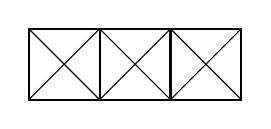
\begin{tikzpicture}[scale=0.9]
\foreach \x in {0,1,2} {\draw[thick] (\x,0) rectangle (\x+1,1); \draw (\x,0)--(\x+1,1); \draw (\x,1)--(\x+1,0);}
\end{tikzpicture}}
\optstwo{28 triangles, 3 squares}{24 triangles, 5 squares}{28 triangles, 5 squares}{24 triangles, 3 squares}
\answer{C}{28 triangles, 5 squares}
\begin{explain}
\textbf{Triangles.} Each square with both diagonals contains 4 small triangles and 4 half-square triangles, i.e.\ $8\times3=24$. Across each pair of adjacent squares, the diagonals meeting at the shared top (or bottom) corner form a larger triangle on the base of two squares: $2$ pairs $\times$ $2$ (top and bottom) $=4$. Total $=\mathbf{28}$.

\textbf{Squares.} There are 3 visible squares. Around each shared vertical edge, the diagonals of the two neighbouring squares form a tilted square (a diamond), which adds 2 more. Total $=\mathbf{5}$.
\end{explain}
\end{question}

\begin{question}{37}
{`CENSUS' data are:\par}
\optstwo{Primary data}{Secondary data}{Simulated data}{Cross-sectional data}
\answer{A}{Primary data}
\begin{explain}
The official key treats \textbf{census data as primary data}: they are collected directly, first-hand, from every unit of the population by the census organisation. (For other researchers who later use published census tables, the same data become secondary data.)
\end{explain}
\end{question}

\begin{question}{38}
{The data collected on various blood groups of a population of a city is:\par}
\optstwo{Quantitative data}{Qualitative data}{Continuous data}{Descriptive data}
\answer{B}{Qualitative data}
\begin{explain}
Blood groups (A, B, AB, O) are \textbf{categories}, not measurements, so they are \textbf{qualitative (nominal)} data.
\end{explain}
\end{question}

\begin{question}{39}
{The following pie diagram shows the amounts that a family spends on: Food, clothing, rent and miscellaneous expenditure and savings. If the monthly income of the family is 60,000, then monthly savings are:\par}
\qfigure{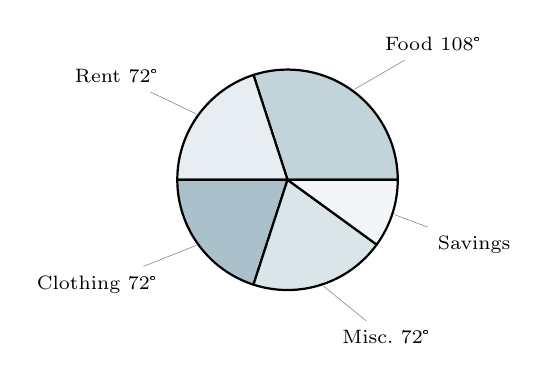
\begin{tikzpicture}\pie[radius=1.4,text=pin,font=\scriptsize,hide number,color={brand!25,brand!10,brand!35,brand!15,brand!5}]{30/Food 108\textdegree,20/Rent 72\textdegree,20/Clothing 72\textdegree,20/Misc.\ 72\textdegree,10/Savings}\end{tikzpicture}}
\optsfour{3,000}{6,000}{7,500}{9,000}
\answer{B}{6,000}
\begin{explain}
Savings $=360^\circ-(108+72+72+72)^\circ=36^\circ$.
\[\text{Savings}=\frac{36}{360}\times60{,}000=\mathbf{6{,}000}\]
\end{explain}
\end{question}

\begin{question}{40}
{The following bar diagram shows the registration of CARS and total vehicles during the first six months of the year 2004 in DELHI:\par}
\qfigure{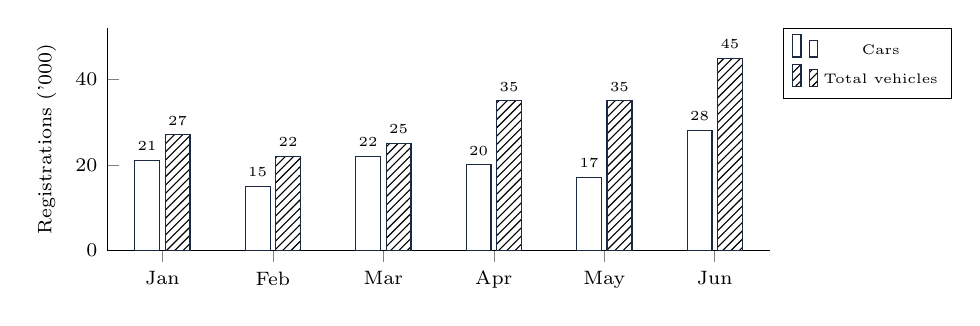
\begin{tikzpicture}
\begin{axis}[ybar,width=10cm,height=4.4cm,bar width=9pt,ymin=0,ymax=52,
  symbolic x coords={Jan,Feb,Mar,Apr,May,Jun},xtick=data,legend style={font=\tiny,at={(1.02,1)},anchor=north west},
  nodes near coords,every node near coord/.append style={font=\tiny},tick label style={font=\scriptsize},
  ylabel={\scriptsize Registrations ('000)},axis x line*=bottom,axis y line*=left]
\addplot[fill=white,draw=ink] coordinates {(Jan,21) (Feb,15) (Mar,22) (Apr,20) (May,17) (Jun,28)};
\addplot[pattern=north east lines,draw=ink] coordinates {(Jan,27) (Feb,22) (Mar,25) (Apr,35) (May,35) (Jun,45)};
\legend{Cars,Total vehicles}
\end{axis}
\end{tikzpicture}}
What was the percentage increase in registration of CARS from MAY to JUNE 2004?
\optsfour{64.2\%}{64.5\%}{64.7\%}{64.9\%}
\answer{C}{64.7\%}
\begin{explain}
Cars: May $=17$ thousand, June $=28$ thousand.
\[\frac{28-17}{17}\times100=\frac{11}{17}\times100\approx\mathbf{64.7\%}\]
\end{explain}
\end{question}

\begin{question}{41}
{The number of male and female students registered for their Ph.D. programme in various faculties along with their total strength in years 2006-2015 can be `best' represented by a:\par}
\optstwo{Simple bar diagram}{Multiple bar diagram}{Histogram}{Pie diagram}
\answer{B}{Multiple bar diagram}
\begin{explain}
The data show male and female numbers (and totals) for each faculty over several years, i.e.\ several related quantities side by side for each category. A \textbf{multiple (grouped) bar diagram} represents this best.
\why{A simple bar diagram shows one variable; a histogram is for continuous frequency distributions; a pie diagram shows the parts of one whole.}
\end{explain}
\end{question}

\begin{question}{42}
{Raw data collected on: height, weight, BMI and age can be:\par}
\optstwo{classified}{tabulated}{both classified and tabulated}{categorized}
\answer{C}{both classified and tabulated}
\begin{explain}
Raw data on height, weight, BMI and age can first be \textbf{classified} (grouped into classes) and then \textbf{tabulated} (arranged in rows and columns) for analysis.
\end{explain}
\end{question}

\begin{question}{43}
{Which of the following is the Web browser?\par}
\optsfour{Windows 7}{C++ Language}{Google Chrome}{Tally}
\answer{C}{Google Chrome}
\begin{explain}
\textbf{Google Chrome} is a web browser.
\why{Windows 7 is an operating system, C++ is a programming language, and Tally is accounting software.}
\end{explain}
\end{question}

\begin{question}{44}
{What is the full form of MOOC?\par}
\optstwo{Most Organised Offline Courses}{Modern Online Office Courses}{Massive Open Online Courses}{Massive Office Order Cell}
\answer{C}{Massive Open Online Courses}
\begin{explain}
\textbf{MOOC} is \textbf{Massive Open Online Course}, an online course open to unlimited participants (e.g.\ SWAYAM, Coursera, edX).
\end{explain}
\end{question}

\begin{question}{45}
{Which number system is used to store data and perform calculation in computers?\par}
\optsfour{Octal}{Binary}{Decimal}{Hexadecimal}
\answer{B}{Binary}
\begin{explain}
Computers store data and compute in the \textbf{binary} number system (0 and 1), matching the two states of electronic circuits.
\end{explain}
\end{question}

\begin{question}{46}
{Which law protects the crimes through Internet?\par}
\optsfour{IT Law}{Common Law}{Cyber Law}{Natural Law}
\answer{C}{Cyber Law}
\begin{explain}
Crimes committed through computers and the Internet are dealt with by \textbf{cyber law}. In India this is chiefly the Information Technology Act, 2000 (amended in 2008).
\end{explain}
\end{question}

\begin{question}{47}
{ATM stands for:\par}
\optstwo{All Time Money}{Auto Teller Machine}{Automated Teller Machine}{Arithmetic Teller Machine}
\answer{C}{Automated Teller Machine}
\begin{explain}
\textbf{ATM} is \textbf{Automated Teller Machine}.
\end{explain}
\end{question}

\begin{question}{48}
{Personal data is often transmitted over the internet. One method of securing the data before transmission is:\par}
\optstwo{Filtering}{Using encryption}{Using firewall}{Streaming}
\answer{B}{Using encryption}
\begin{explain}
\textbf{Encryption} converts data into a coded (cipher) form that only authorised parties with the key can read, e.g.\ SSL/TLS (HTTPS). This secures personal data in transit.
\end{explain}
\end{question}

\begin{question}{49}
{Chemistry of corrosion is:\par}
\optstwo{Electrochemical Phenomenon}{Physiochemical Phenomenon}{Reduction}{Hydrothermal Reaction}
\answer{A}{Electrochemical Phenomenon}
\begin{explain}
Corrosion (e.g.\ rusting of iron) is an \textbf{electrochemical} process. Anodic and cathodic regions form on the metal surface, with oxidation $\mathrm{Fe}\rightarrow\mathrm{Fe}^{2+}+2e^-$ and reduction of oxygen, and moisture acts as the electrolyte.
\end{explain}
\end{question}

\begin{question}{50}
{Which is not correct for `green chemistry'?\par}
\optsone{Design benign chemicals}{Design for non-degradation}{Design to reduce the use and generation of hazardous substances}{Design for strategic pathway to build a sustainable future}
\answer{B}{Design for non-degradation}
\begin{explain}
The \emph{12 Principles of Green Chemistry} (Anastas \& Warner) include designing safer (benign) chemicals, reducing hazardous substances and \textbf{designing for degradation}: products should break down into harmless substances after use. ``Design for \emph{non}-degradation'' is therefore not correct.
\end{explain}
\end{question}

\begin{question}{51}
{The work of Hargobind Khorana in which he got Nobel Prize was:\par}
\optstwo{Penicillin}{Sulpha drug}{Cracking of genetic code}{Pairing of nucleotide base}
\answer{C}{Cracking of genetic code}
\begin{explain}
\textbf{Har Gobind Khorana} shared the 1968 Nobel Prize in Physiology or Medicine (with Nirenberg and Holley) for the \textbf{interpretation (cracking) of the genetic code} and its role in protein synthesis.
\end{explain}
\end{question}

\begin{question}{52}
{Amount of organic pollutants found in surface water is measured by:\par}
\optstwo{COD (Chemical Oxygen Demand)}{Energy efficient batteries}{3-D printed structure}{Gas sensitive semiconductor technology}
\answer{A}{COD (Chemical Oxygen Demand)}
\begin{explain}
\textbf{COD (Chemical Oxygen Demand)} measures the oxygen needed to chemically oxidise organic pollutants in water. It is an indicator of organic pollution (together with BOD).
\end{explain}
\end{question}

\begin{question}{53}
{Bubblegum contains:\par}
\optstwo{Natural Rubber}{Synthetic Rubber}{Synthetic Styrenebutadiene Rubber}{Styrene Maleic Anhydride}
\answer{C}{Synthetic Styrenebutadiene Rubber}
\begin{explain}
Chewing-gum and bubble-gum bases use synthetic elastomers, mainly \textbf{styrene--butadiene rubber (SBR)} and polyisobutylene, which give them stretch and elasticity.
\end{explain}
\end{question}

\begin{question}{54}
{To raise global awareness, which day every year we celebrate Environment Day?\par}
\optsfour{10th May}{13th March}{5th June}{17th January}
\answer{C}{5th June}
\begin{explain}
\textbf{World Environment Day} is celebrated on \textbf{5 June} every year (UNEP; first observed in 1974, commemorating the 1972 Stockholm Conference).
\end{explain}
\end{question}

\begin{question}{55}
{What is the main objective of NAAC in India?\par}
\optstwo{Establishing Universities}{Evaluating Universities}{Accrediting Universities}{Funding Universities}
\answer{C}{Accrediting Universities}
\begin{explain}
The main objective of \textbf{NAAC} is the \textbf{assessment and accreditation} of higher-education institutions.
\end{explain}
\end{question}

\begin{question}{56}
{"Gujarat Vidyapith", Ahmedabad is a:\par}
\optstwo{Central University}{State University}{Private University}{Deemed University}
\answer{D}{Deemed University}
\begin{explain}
\textbf{Gujarat Vidyapith}, founded by Mahatma Gandhi in 1920, is a \textbf{deemed university} (since 1963).
\end{explain}
\end{question}

\begin{question}{57}
{Which of the following is a popular programme for promoting science and technology supported by Department of Science and Technology (DST), Govt. of India?\par}
\optsfour{INSPIRE}{SCOPE}{PMOST}{SSA}
\answer{A}{INSPIRE}
\begin{explain}
\textbf{INSPIRE} (Innovation in Science Pursuit for Inspired Research, 2008) is DST's flagship programme to attract young talent to science through scholarships, fellowships and awards (e.g.\ INSPIRE-MANAK).
\end{explain}
\end{question}

\begin{question}{58}
{Which of the following is a Central University?\par}
\optstwo{Gujarat University}{Mohanlal Sukhadia University}{Banaras Hindu University}{Mumbai University}
\answer{C}{Banaras Hindu University}
\begin{explain}
\textbf{Banaras Hindu University} (founded 1916 by Madan Mohan Malaviya) is a central university.
\why{Gujarat University, Mohanlal Sukhadia University (Udaipur) and the University of Mumbai are state universities.}
\end{explain}
\end{question}

\begin{question}{59}
{Which of the following is an Exclusive Women University?\par}
\optstwo{University of Delhi}{SNDT University}{Gujarat Vidyapeeth}{Visva-Bharati University}
\answer{B}{SNDT University}
\begin{explain}
\textbf{SNDT Women's University}, Mumbai (founded 1916 by Dhondo Keshav Karve) is India's first exclusively women's university.
\end{explain}
\end{question}

\begin{question}{60}
{For which field the Vikram Sarabhai Awards are given?\par}
\optstwo{Biological Research}{Agricultural Research}{Space Research}{Mathematical Research}
\answer{A}{Biological Research}
\keynote{The official key gives (A). Students should note that the best-known \emph{Vikram Sarabhai Research Award} (Physical Research Laboratory) and the \emph{Vikram Sarabhai Memorial Award} (COSPAR) relate to space science. Answer as per the key in the exam context.}
\begin{explain}
Awards named after Dr.~Vikram Sarabhai, the father of India's space programme, are given in several fields of science. The official GSET key identifies the field as \textbf{biological research}.
\end{explain}
\end{question}

\paperchapter{October 2014}{October 2014}{A}{60}{GSET 2014}
\keytable{\kcell{1}{C} & \kcell{2}{A} & \kcell{3}{C} & \kcell{4}{B} & \kcell{5}{B} & \kcell{6}{D} & \kcell{7}{D} & \kcell{8}{A} & \kcell{9}{C} & \kcell{10}{A} \\
\kcell{11}{D} & \kcell{12}{A} & \kcell{13}{D} & \kcell{14}{C} & \kcell{15}{B} & \kcell{16}{B} & \kcell{17}{D} & \kcell{18}{B} & \kcell{19}{C} & \kcell{20}{C} \\
\kcell{21}{C} & \kcell{22}{B} & \kcell{23}{C} & \kcell{24}{D} & \kcell{25}{B} & \kcell{26}{A} & \kcell{27}{B} & \kcell{28}{A} & \kcell{29}{D} & \kcell{30}{D} \\
\kcell{31}{C} & \kcell{32}{B} & \kcell{33}{C} & \kcell{34}{B} & \kcell{35}{A} & \kcell{36}{C} & \kcell{37}{A} & \kcell{38}{A} & \kcell{39}{B} & \kcell{40}{D} \\
\kcell{41}{A} & \kcell{42}{C} & \kcell{43}{A} & \kcell{44}{D} & \kcell{45}{A} & \kcell{46}{B} & \kcell{47}{D} & \kcell{48}{C} & \kcell{49}{A} & \kcell{50}{D} \\
\kcell{51}{C} & \kcell{52}{A} & \kcell{53}{B} & \kcell{54}{C} & \kcell{55}{A} & \kcell{56}{A} & \kcell{57}{C} & \kcell{58}{D} & \kcell{59}{A} & \kcell{60}{D}}
\begin{question}{1}
{Which of the following is least desirable outcome of teaching in higher education?\par}
\optsone{Enhancement of independent thinking of students}{Increase in students probing skills}{Good preparation for appearing in examination}{Helping students to think out of the box}
\answer{C}{Good preparation for appearing in examination}
\begin{explain}
Higher education aims at independent thinking, inquiry (probing), creativity and ``thinking out of the box''. Mere \textbf{preparation for examinations} is the \emph{least desirable} outcome: it encourages rote learning.
\end{explain}
\end{question}

\begin{question}{2}
{Here some qualities of the teachers are presented. Which one of the following combination of qualities is most suitable in an effective teacher?\newline (1) Knowledge of subject matter\newline (2) Effective oral communication\newline (3) Pleasant presence\newline (4) To be object of respect of the students\newline (5) To be object of respect of the leaders of the society\par}
\optsfour{1, 2, 4}{1, 2, 3}{2, 3, 4}{1, 2, 5}
\answer{A}{1, 2, 4}
\begin{explain}
An effective teacher combines \textbf{mastery of the subject (1)}, \textbf{effective oral communication (2)} and \textbf{the respect of students (4)}. Being respected by society's leaders (5) and a pleasant presence (3) are not essential qualities of teaching. The answer is 1, 2, 4.
\end{explain}
\end{question}

\begin{question}{3}
{Which of the following technique of teaching is more suitable for developing creativity in students?\par}
\optstwo{Lecture}{Demonstration}{Field study}{Providing self-learning material}
\answer{C}{Field study}
\begin{explain}
\textbf{Field study} puts learners in real, open-ended situations where they observe, explore, question and produce original ideas, which develops creativity.
\why{Lecture and demonstration are teacher-centred; self-learning material is structured and convergent.}
\end{explain}
\end{question}

\begin{question}{4}
{Assessment that take place during process of teaching in classroom is:\par}
\optstwo{Classroom assessment}{Formative assessment}{Summative assessment}{Comprehensive assessment}
\answer{B}{Formative assessment}
\begin{explain}
\textbf{Formative assessment} takes place \emph{during} the teaching--learning process to monitor progress and provide feedback (assessment \emph{for} learning). Summative assessment comes at the end.
\end{explain}
\end{question}

\begin{question}{5}
{Which of the following helps learner to learn better?\par}
\optstwo{Giving notes}{Discussion in the class}{Explaining the main points}{Knowledge of the teacher}
\answer{B}{Discussion in the class}
\begin{explain}
\textbf{Classroom discussion} involves learners actively: they express, question, listen and build on others' ideas. This deepens understanding far more than passively receiving notes or explanations.
\end{explain}
\end{question}

\begin{question}{6}
{In constructivist approach, learner is viewed as:\par}
\optstwo{responding being}{evolving being}{emotional being}{exploring being}
\answer{D}{exploring being}
\begin{explain}
In \textbf{constructivism} (Piaget, Vygotsky, Bruner) the learner is an active \textbf{explorer} who constructs knowledge through exploration and experience. The learner is not a passive responder.
\end{explain}
\end{question}

\begin{question}{7}
{When each unit of a population has an equal likelihood of being selected, the method of sampling is called:\par}
\optstwo{A non-random sampling}{A quota sampling}{A snowball sampling}{A random sampling}
\answer{D}{A random sampling}
\begin{explain}
When every unit of the population has an \textbf{equal (and independent) chance} of selection, the method is \textbf{random (probability) sampling}.
\end{explain}
\end{question}

\begin{question}{8}
{A researcher wants to study the future of an Institution. For the study which tool is most appropriate for him/her?\par}
\optsfour{Questionnaire}{Observation}{Interview}{Rating Scale}
\answer{A}{Questionnaire}
\begin{explain}
Studying the future of an institution requires the considered views of many stakeholders and experts. A \textbf{questionnaire} can collect these systematically from a large, spread-out group; futures studies such as the \emph{Delphi technique} use successive rounds of questionnaires to build consensus about the future.
\end{explain}
\end{question}

\begin{question}{9}
{Hypothesis cannot be stated in:\par}
\optstwo{Null and question form}{Declarative terms}{General terms}{Directional form}
\answer{C}{General terms}
\begin{explain}
A research hypothesis is a specific, testable statement. It can be declarative, null or directional, but it \textbf{cannot be in question form}. (A question is a research \emph{question}, not a hypothesis.)
\end{explain}
\end{question}

\begin{question}{10}
{A text taken from a source is placed in a research report without providing reference is called as:\par}
\optstwo{Plagiarism}{Popularism}{Perfectionism}{Post-referencism}
\answer{A}{Plagiarism}
\begin{explain}
Presenting someone else's text without acknowledging the source is \textbf{plagiarism}.
\end{explain}
\end{question}

\begin{question}{11}
{What is the correct sequence of steps in research?\par}
\optsone{Sampling; identification of problem; development of tools; data analysis; data collection}{Identification of problem; development of tools; sampling; data collection; data analysis}{Development of tools; identification of problem; data analysis; sampling; data collection}{Identification of problem; sampling; development of tools; data collection; data analysis}
\answer{D}{Identification of problem; sampling; development of tools; data collection; data analysis}
\begin{explain}
The logical research sequence: \textbf{identify the problem $\rightarrow$ select the sample $\rightarrow$ develop tools $\rightarrow$ collect data $\rightarrow$ analyse data}, which is option (D).
\tip{Some texts place tool development before sampling. Either way, the problem comes first and data analysis comes after data collection.}
\end{explain}
\end{question}

\begin{question}{12}
{Practitioners such as teachers, counsellors and other professionals attempt to find solutions to some issues in a systematic manner. This is known as:\par}
\optstwo{Action Research}{Basic Research}{Applied Research}{Developmental Research}
\answer{A}{Action Research}
\begin{explain}
\textbf{Action research} (Stephen Corey applied it to education) is carried out by practitioners such as teachers and counsellors to solve \emph{their own immediate problems} systematically and improve practice.
\end{explain}
\end{question}

\begin{context}
\textbf{Read the paragraph and answer the Question Nos.~13--18.}\par\smallskip
Adolescence is a period of rapid growth and development bridging childhood and adulthood. Practicing healthy eating behaviour is one of the most important factors to meet the nutritional needs of adolescents. Proper eating behaviours that are learned in early life are maintained in adulthood thus reducing the risk of major chronic diseases. Physical and psychological changes occurring during this period usually significantly influence their dietary behaviours. As teens become more independent, they make more of their own food choices. However, being influenced by a massive amount of factors (biological, social, physical, economic, psychological beliefs and knowledge about food) and changing of lifestyle may affect their dietary choices and eating behaviour, thus making them fail to adhere to healthy eating practices. Peer pressure in colleges leads adolescents to eating non-nutritional foods like pizzas and burgers. Due to irregular college schedules, intake of caffeinated drinks increases and water intake reduces. Poor nutrition can lead to reduced concentration in studies, low stamina, depression or poor posture.
\end{context}
\begin{question}{13}
{Adolescents succumb to unhealthy dietary habits due to:\par}
\optstwo{Physical and psychological changes}{Independence in making food choices}{Changing lifestyle}{Peer pressure in colleges}
\answer{D}{Peer pressure in colleges}
\begin{explain}
The official key gives \textbf{peer pressure in colleges}: ``Peer pressure in colleges \textbf{leads} adolescents to eating non-nutritional foods like pizzas and burgers.'' This is the direct cause the passage names for giving in to unhealthy foods.
\end{explain}
\end{question}

\begin{question}{14}
{Unhealthy dietary habits means:\par}
\optstwo{Eating pizzas and burgers}{Caffeinated drinks}{Poor nutritional diet}{Drinking less water}
\answer{C}{Poor nutritional diet}
\begin{explain}
Pizzas, burgers, caffeine and less water are examples. What they add up to is a \textbf{poor nutritional diet}, the general meaning of unhealthy dietary habits.
\end{explain}
\end{question}

\begin{question}{15}
{Reduced concentration in studies is because of:\par}
\optsone{Nature of Adolescent period}{Not being able to meet nutritional needs}{Influence of factors like biological and psychological}{Eating of foods like pizzas and burgers}
\answer{B}{Not being able to meet nutritional needs}
\begin{explain}
``\textbf{Poor nutrition} can lead to reduced concentration in studies.'' Poor nutrition means \textbf{not being able to meet nutritional needs}.
\end{explain}
\end{question}

\begin{question}{16}
{The author marks adolescent as bridging childhood and adulthood because it is a:\par}
\optsone{Period of independence in making dietary choices}{Period of physical and psychological changes}{Period of changing lifestyle}{Period of peer pressure}
\answer{B}{Period of physical and psychological changes}
\begin{explain}
Adolescence bridges childhood and adulthood because it is a period of rapid growth, i.e.\ \textbf{physical and psychological changes}.
\end{explain}
\end{question}

\begin{question}{17}
{What is the meaning of dietary behaviour?\par}
\optstwo{Taking different types of diet}{Taking caffeinated drinks}{Knowledge of different types of diets}{Making choices about diet}
\answer{D}{Making choices about diet}
\begin{explain}
Dietary behaviour refers to how a person \textbf{makes choices about diet}: what, when and how much to eat (``as teens become more independent, they make more of their own food choices'').
\end{explain}
\end{question}

\begin{question}{18}
{As per the author, how does dietary behaviour in adolescence affect health in adulthood?\par}
\optsone{Major chronic diseases are transferred from early stage to adulthood}{The seed of ill health in adulthood is sown by diet in early stages}{Dietary habits of adolescence are carried out in adulthood}{Dietary habits are maintained throughout life}
\answer{B}{The seed of ill health in adulthood is sown by diet in early stages}
\begin{explain}
``Proper eating behaviours that are learned in early life are maintained in adulthood, thus reducing the risk of major chronic diseases.'' By the same logic, poor eating in adolescence \textbf{sows the seeds of ill health in adulthood}.
\end{explain}
\end{question}

\begin{question}{19}
{Which one of the following functions a sender would perform during communication?\par}
\optsfour{Decoding}{Feedback}{Encoding}{Reception}
\answer{C}{Encoding}
\begin{explain}
The sender \textbf{encodes}: converts ideas into symbols (words, signs). Decoding and reception are the receiver's functions; feedback is the receiver's response.
\end{explain}
\end{question}

\begin{question}{20}
{Given the following components of communication, which combination represents classroom communication best?\newline (i) Individual to Individual\newline (ii) Individual to Group\newline (iii) Group to Individual\newline (iv) Group to Group\par}
\optstwo{(i) and (ii)}{(ii) and (iv)}{(i), (ii) and (iii)}{(iii) and (iv)}
\answer{C}{(i), (ii) and (iii)}
\begin{explain}
In a classroom the teacher speaks to individual students \textbf{(i)} and to the whole class \textbf{(ii)}, and the class or a group responds to the teacher \textbf{(iii)}. The answer is (i), (ii) and (iii).
\end{explain}
\end{question}

\begin{question}{21}
{In order to protect sensitive matter sent through e-mail, the sender should:\par}
\optstwo{write the matter in another language}{not provide self-address}{encrypt the matter}{not inform any one about this matter}
\answer{C}{encrypt the matter}
\begin{explain}
\textbf{Encryption} converts the content into a code that only the intended recipient (with the key) can read, protecting sensitive e-mail matter.
\end{explain}
\end{question}

\begin{question}{22}
{A manager of an organisation transfers a message to his/her subordinates. Which type of communication is this?\par}
\optsfour{Diagonal}{Downward}{Horizontal}{Upward}
\answer{B}{Downward}
\begin{explain}
Communication from a superior to subordinates is \textbf{downward communication}.
\end{explain}
\end{question}

\begin{question}{23}
{In what type of communication, sender transfers message using body movements?\par}
\optsfour{Verbal}{Written}{Gestural}{Silence}
\answer{C}{Gestural}
\begin{explain}
Communication through body movements (gestures, postures) is \textbf{gestural} (kinesic) non-verbal communication.
\end{explain}
\end{question}

\begin{question}{24}
{Arrange the elements of communication in a sequential order:\par}
\optstwo{Sender, receiver, message, feedback}{Sender, message, feedback, receiver}{Sender, feedback, message, receiver}{Sender, message, receiver, feedback}
\answer{D}{Sender, message, receiver, feedback}
\begin{explain}
\textbf{Sender $\rightarrow$ Message $\rightarrow$ Receiver $\rightarrow$ Feedback}.
\end{explain}
\end{question}

\begin{question}{25}
{If 2 $\times$ 7 = 41, 4 $\times$ 3 = 21, 5 $\times$ 5 = 52, then 3 $\times$ 6 = \blank{}\par}
\optsfour{39}{81}{121}{208}
\answer{B}{81}
\begin{explain}
The product is written with its digits reversed:
\[2\times7=14\rightarrow41,\qquad4\times3=12\rightarrow21,\qquad5\times5=25\rightarrow52\]
\[3\times6=18\rightarrow\mathbf{81}\]
\end{explain}
\end{question}

\begin{question}{26}
{Arrange in a meaningful sequence:\newline (1) Status\newline (2) Service\newline (3) Income\newline (4) Settlement\newline (5) Study\par}
\optsfour{5 $\rightarrow$ 2 $\rightarrow$ 3 $\rightarrow$ 1 $\rightarrow$ 4}{5 $\rightarrow$ 4 $\rightarrow$ 3 $\rightarrow$ 2 $\rightarrow$ 1}{4 $\rightarrow$ 3 $\rightarrow$ 2 $\rightarrow$ 1 $\rightarrow$ 5}{3 $\rightarrow$ 1 $\rightarrow$ 2 $\rightarrow$ 4 $\rightarrow$ 5}
\answer{A}{5 $\rightarrow$ 2 $\rightarrow$ 3 $\rightarrow$ 1 $\rightarrow$ 4}
\begin{explain}
A person first \textbf{studies (5)}, then gets \textbf{service} (a job) (2), which brings \textbf{income (3)}, which gives \textbf{status (1)}, and finally \textbf{settlement (4)} in life. The order is 5 $\rightarrow$ 2 $\rightarrow$ 3 $\rightarrow$ 1 $\rightarrow$ 4.
\end{explain}
\end{question}

\begin{question}{27}
{Put the correct number in the box:\newline 0, 2, 6, 12, [ ], 30\par}
\optsfour{18}{20}{28}{14}
\answer{B}{20}
\begin{explain}
Each term is $n(n-1)$: $1\cdot0=0$, $2\cdot1=2$, $3\cdot2=6$, $4\cdot3=12$, $5\cdot4=\mathbf{20}$, $6\cdot5=30$. (Differences: 2, 4, 6, 8, 10.)
\end{explain}
\end{question}

\begin{question}{28}
{If NOT is encoded as 415102, then SRP will have the code:\par}
\optsfour{918161}{191816}{1986}{689}
\answer{A}{918161}
\begin{explain}
Each letter is replaced by its alphabet position written \emph{in reverse}: N $=14\rightarrow41$, O $=15\rightarrow51$, T $=20\rightarrow02$, giving 415102.
SRP: S $=19\rightarrow91$, R $=18\rightarrow81$, P $=16\rightarrow61$, giving \textbf{918161}.
\end{explain}
\end{question}

\begin{question}{29}
{If 2 $\times$ 6 = 7, 4 $\times$ 2 = 27, 7 $\times$ 3 = 144, then 5 $\times$ 8 = \blank{}\par}
\optsfour{140}{142}{143}{144}
\answer{D}{144}
\keynote{No single consistent rule fits all three given examples. Students should record the official answer and not spend exam time on such items.}
\begin{explain}
The official key gives \textbf{(D) 144}. The first two examples fit $(b+1)^{a-1}$: $(6+1)^{2-1}=7$ and $(2+1)^{4-1}=27$. The third ($7\times3=144$) does not fit that rule, and no rule gives any of the options for $5\times8$ unambiguously. The question is best treated as defective; answer according to the key.
\end{explain}
\end{question}

\begin{question}{30}
{Complete the sequence by filling the blank using correct number:\newline 0, 2, 12, \blank{}, 80\par}
\optsfour{66}{52}{48}{36}
\answer{D}{36}
\begin{explain}
Each term is $n^2(n+1)$ for $n=0,1,2,3,4$: $0$, $1\cdot2=2$, $4\cdot3=12$, $9\cdot4=\mathbf{36}$, $16\cdot5=80$.
\end{explain}
\end{question}

\begin{question}{31}
{Put the correct number at "?" and complete the sequence:\newline A(4), F(9), M(?), Q(20)\par}
\optsfour{12}{14}{16}{17}
\answer{C}{16}
\begin{explain}
The number is the letter's position $+3$: A(1)$+3=4$, F(6)$+3=9$, M(13)$+3=\mathbf{16}$, Q(17)$+3=20$.
\end{explain}
\end{question}

\begin{question}{32}
{Complete the sequence by putting the correct letter:\newline C, H, M, \blank{}, W\par}
\optsfour{O}{R}{Q}{T}
\answer{B}{R}
\begin{explain}
The letters advance by 5: C(3), H(8), M(13), \textbf{R(18)}, W(23).
\end{explain}
\end{question}

\begin{context}
There are total 400 candidates applying for admission to one of the courses C1, C2, C3, C4 and C5, for study. The given table shows \% number of all 400 candidates admitted to these courses. Based on this table, answer the following questions (33--35):
\begin{center}
\begin{tabular}{lcccccc}\toprule \textbf{Course} & C1 & C2 & C3 & C4 & C5\\\midrule
\textbf{\% admitted} & 15 & 10 & 25 & 30 & 20\\
\textbf{Number} (of 400) & 60 & 40 & 100 & 120 & 80\\\bottomrule
\end{tabular}
\end{center}
\end{context}
\begin{question}{33}
{The sequence in increasing order of number of candidates in these courses, is:\par}
\optstwo{30, 65, 85, 90, 130}{35, 60, 80, 105, 120}{40, 60, 80, 100, 120}{50, 60, 70, 90, 130}
\answer{C}{40, 60, 80, 100, 120}
\begin{explain}
The numbers are 60, 40, 100, 120 and 80. In increasing order: \textbf{40, 60, 80, 100, 120}.
\end{explain}
\end{question}

\begin{question}{34}
{The ratio of number of candidates in course C3 to the number of candidates in course C5 is:\par}
\optsfour{3 : 2}{5 : 4}{6 : 4}{6 : 5}
\answer{B}{5 : 4}
\begin{explain}
C3 : C5 $=100:80=\mathbf{5:4}$ (equivalently $25\%:20\%$).
\end{explain}
\end{question}

\begin{question}{35}
{The sequence of admitted number of candidates, in order of courses C1 to C5, is:\par}
\optstwo{60, 40, 100, 120, 80}{50, 80, 100, 120, 50}{100, 50, 30, 130, 90}{90, 50, 30, 130, 100}
\answer{A}{60, 40, 100, 120, 80}
\begin{explain}
C1 to C5 in order: $15\%, 10\%, 25\%, 30\%, 20\%$ of 400 $=$ \textbf{60, 40, 100, 120, 80}.
\end{explain}
\end{question}

\begin{context}
The following graph records the number of employees who joined and left a company in the month of April, from the period 2005 to 2009. The initial number of employees in the company is 1000. Based on this graph, answer the questions 36--38.
\begin{center}
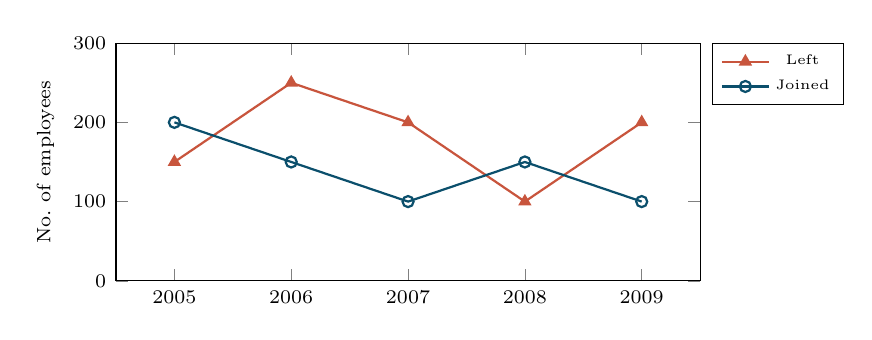
\begin{tikzpicture}
\begin{axis}[width=9cm,height=4.6cm,xmin=2004.5,xmax=2009.5,ymin=0,ymax=300,xtick={2005,...,2009},
  x tick label style={/pgf/number format/1000 sep=},tick label style={font=\scriptsize},
  ylabel={\scriptsize No.\ of employees},legend style={font=\tiny,at={(1.02,1)},anchor=north west}]
\addplot[mark=triangle*,thick,accent] coordinates {(2005,150) (2006,250) (2007,200) (2008,100) (2009,200)};
\addplot[mark=o,thick,brand] coordinates {(2005,200) (2006,150) (2007,100) (2008,150) (2009,100)};
\legend{Left,Joined}
\end{axis}
\end{tikzpicture}
\end{center}
\end{context}
\begin{question}{36}
{The ratio of total number of employees in 2005 to the total number of employees in 2006 is:\par}
\optsfour{11 : 10}{20 : 17}{21 : 19}{13 : 11}
\answer{C}{21 : 19}
\begin{explain}
Running total (start $=1000$):
\begin{center}\small
\begin{tabular}{lcccc}\toprule Year & Joined & Left & Net & Employees\\\midrule
2005 & 200 & 150 & $+50$ & \textbf{1050}\\ 2006 & 150 & 250 & $-100$ & \textbf{950}\\ 2007 & 100 & 200 & $-100$ & 850\\ 2008 & 150 & 100 & $+50$ & 900\\ 2009 & 100 & 200 & $-100$ & 800\\\bottomrule
\end{tabular}
\end{center}
2005 : 2006 $=1050:950=\mathbf{21:19}$.
\end{explain}
\end{question}

\begin{question}{37}
{How many employees were serving the company in 2005?\par}
\optsfour{1050}{1200}{1150}{900}
\answer{A}{1050}
\begin{explain}
$1000+200-150=\mathbf{1050}$ (see the table in Q.~36).
\end{explain}
\end{question}

\begin{question}{38}
{In which year, the number of employees was maximum?\par}
\optsfour{2005}{2007}{2008}{2009}
\answer{A}{2005}
\begin{explain}
The totals are 1050, 950, 850, 900 and 800, so the maximum is in \textbf{2005}.
\end{explain}
\end{question}

\begin{question}{39}
{Which of the following diagrams indicates all possible relations amongst milk-M, Sugar-S, Tea-T and Coffee-F?\par}
\optsfour{\tikz[baseline=-0.5ex,scale=0.32]{\draw (0,1.05) circle(1); \draw (-1.05,0) circle(1); \draw (1.05,0) circle(1); \draw (0,-1.05) circle(1);}}{\tikz[baseline=-0.5ex,scale=0.32]{\draw (0,0.8) circle(1); \draw (-0.8,0) circle(1); \draw (0.8,0) circle(1); \draw (0,-0.8) circle(1);}}{\tikz[baseline=-0.5ex,scale=0.32]{\draw (0,0) circle(2); \draw (0.3,0) circle(1.3); \draw (0.5,0.5) circle(0.4); \draw (0.5,-0.5) circle(0.4);}}{\tikz[baseline=-0.5ex,scale=0.32]{\draw (0,0) circle(2); \draw (0,-0.2) circle(1.4); \draw (-0.45,-0.5) circle(0.4); \draw (0.45,-0.5) circle(0.4);}}
\answer{B}{\tikz[baseline=-0.5ex,scale=0.32]{\draw (0,0.8) circle(1); \draw (-0.8,0) circle(1); \draw (0.8,0) circle(1); \draw (0,-0.8) circle(1);}}
\begin{explain}
Milk, sugar, tea and coffee are four different items that are commonly \emph{combined} in any mixture: milk with tea, sugar with coffee, tea with milk and sugar, and so on. To show \textbf{all possible} combinations, including one region common to all four, we need four \textbf{mutually overlapping circles} with a shared central region, as in diagram (B).
\end{explain}
\end{question}

\begin{question}{40}
{(i) Rohit possesses four two-wheelers\newline (ii) Two two-wheelers are black\newline (iii) One two-wheeler is a bicycle\newline From the above statements which conclusion can be drawn?\newline (I) Rohit has black bicycle\newline (II) Rohit has three scooters\newline (III) Rohit does not like black color.\par}
\optstwo{I and II}{III only}{II only}{None of I, II, III is true}
\answer{D}{None of I, II, III is true}
\begin{explain}
From ``two two-wheelers are black'' and ``one is a bicycle'' we cannot tell whether the bicycle is black (I), what the other vehicles are (II), or Rohit's colour preference (III). \textbf{None} of the conclusions follows.
\end{explain}
\end{question}

\begin{question}{41}
{Select the correct number at "?" place:\par}
\qfigure{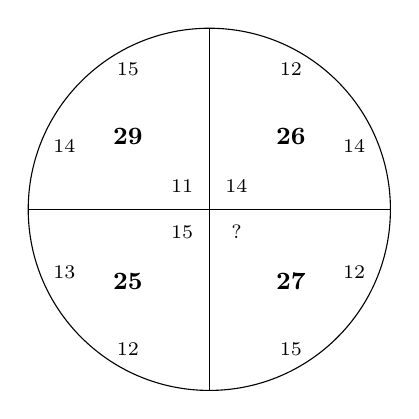
\begin{tikzpicture}[scale=1.15,font=\scriptsize]
\draw (0,0) circle(2); \draw (-2,0)--(2,0); \draw (0,-2)--(0,2);
\node at (-0.9,1.55){15}; \node at (-1.6,0.7){14}; \node[font=\small\bfseries] at (-0.9,0.8){29}; \node at (-0.3,0.25){11};
\node at (0.9,1.55){12}; \node at (1.6,0.7){14}; \node[font=\small\bfseries] at (0.9,0.8){26}; \node at (0.3,0.25){14};
\node at (-1.6,-0.7){13}; \node at (-0.9,-1.55){12}; \node[font=\small\bfseries] at (-0.9,-0.8){25}; \node at (-0.3,-0.25){15};
\node at (1.6,-0.7){12}; \node at (0.9,-1.55){15}; \node[font=\small\bfseries] at (0.9,-0.8){27}; \node at (0.3,-0.25){?};
\end{tikzpicture}}
\optsfour{13}{15}{17}{19}
\answer{A}{13}
\begin{explain}
In each quadrant the centre number is the sum of the two outer numbers, and the inner (corner) number is $40-$ centre:
\begin{center}\small
\begin{tabular}{lccc}\toprule Quadrant & Outer sum & Centre & Inner $=40-$centre\\\midrule
Top-left & $15+14$ & 29 & 11\\ Top-right & $12+14$ & 26 & 14\\ Bottom-left & $13+12$ & 25 & 15\\ Bottom-right & $12+15$ & 27 & \textbf{13}\\\bottomrule
\end{tabular}
\end{center}
\end{explain}
\end{question}

\begin{question}{42}
{If UPE = SNC, then QHD = \blank{}\par}
\optsfour{NKH}{PGE}{OFB}{MKF}
\answer{C}{OFB}
\begin{explain}
Each letter moves two steps back: U$\rightarrow$S, P$\rightarrow$N, E$\rightarrow$C. So QHD $\rightarrow$ \textbf{OFB}.
\end{explain}
\end{question}

\begin{question}{43}
{An attached file with received e-mail is dangerous for:\par}
\optsone{it may carry virus}{computer hard disk gets overloaded}{it costs money to the recepient}{there is no guarantee of reaching to recepient}
\answer{A}{it may carry virus}
\begin{explain}
Attachments from unknown senders may carry \textbf{viruses or malware} (executables, macros) that infect the computer when opened.
\end{explain}
\end{question}

\begin{question}{44}
{In the domain name .org implies:\par}
\optstwo{a website}{operations research group}{commercial website}{an organization}
\answer{D}{an organization}
\begin{explain}
The top-level domain \texttt{.org} denotes an \textbf{organisation}, typically a non-profit. (\texttt{.com} = commercial, \texttt{.edu} = education, \texttt{.gov} = government.)
\end{explain}
\end{question}

\begin{question}{45}
{URL means:\par}
\optstwo{Uniform Resource Locator}{Unique Resource Location}{Universal Recommended Location}{United Resource for Learners}
\answer{A}{Uniform Resource Locator}
\begin{explain}
\textbf{URL} is \textbf{Uniform Resource Locator}.
\end{explain}
\end{question}

\begin{question}{46}
{In a democratic institution most of the communication is:\par}
\optsfour{Vertical}{Horizontal}{Spiral}{Unidimensional}
\answer{B}{Horizontal}
\begin{explain}
In a democratic institution, communication is predominantly \textbf{horizontal}: among peers and equals, participative and consultative, rather than top-down.
\end{explain}
\end{question}

\begin{question}{47}
{Which is odd one?\par}
\optstwo{Microsoft Word}{Microsoft Excel}{Microsoft Access}{Microsoft Windows}
\answer{D}{Microsoft Windows}
\begin{explain}
Word, Excel and Access are \emph{application software} (MS Office). \textbf{Windows} is an \emph{operating system}, so it is the odd one out.
\end{explain}
\end{question}

\begin{question}{48}
{Which one is the largest memory size?\par}
\optsfour{Kilobyte}{Gigabyte}{Terabyte}{Megabyte}
\answer{C}{Terabyte}
\begin{explain}
\textbf{Terabyte} is the largest: TB $>$ GB $>$ MB $>$ KB.
\end{explain}
\end{question}

\begin{question}{49}
{In most of the Indian big cities, the dominant source of air pollution is:\par}
\optstwo{vehicular traffic}{household smoke}{thermal power plant}{suburban trains}
\answer{A}{vehicular traffic}
\begin{explain}
In big Indian cities, \textbf{vehicular traffic} is the dominant source of air pollution (NO$_x$, CO, particulate matter), especially at ground level where people breathe.
\end{explain}
\end{question}

\begin{question}{50}
{Which of the following is not biodegradable?\par}
\optsfour{Vegetables}{Human bones}{Earthworms}{Iron rust}
\answer{D}{Iron rust}
\begin{explain}
Vegetables, bones and earthworms are organic and are decomposed by microbes. \textbf{Iron rust} (hydrated iron oxide) is inorganic and not biodegradable.
\end{explain}
\end{question}

\begin{question}{51}
{Which of the following is least likely to be an effect of Global Warming?\par}
\optsone{Loss of fertile delta regions for agriculture}{Change in global patterns for precipitation}{Decreased rate of photosynthesis in vegetation}{Increased frequency of hurricanes}
\answer{C}{Decreased rate of photosynthesis in vegetation}
\begin{explain}
Global warming is expected to cause loss of deltas (sea-level rise), changed precipitation and more intense hurricanes. Higher CO$_2$ tends to \emph{increase} photosynthesis (the CO$_2$ fertilisation effect), so a \textbf{decreased rate of photosynthesis} is the least likely effect.
\end{explain}
\end{question}

\begin{question}{52}
{Which of the following is used in pencils?\par}
\optsfour{Graphite}{Silicon}{Charcoal}{Phosphorous}
\answer{A}{Graphite}
\begin{explain}
The ``lead'' of a pencil is \textbf{graphite} (a form of carbon) mixed with clay. Pencils contain no lead.
\end{explain}
\end{question}

\begin{question}{53}
{The major cause of Tsunamis in the sea is:\par}
\optsfour{Winds}{Earthquakes}{Volcanoes}{Climate change}
\answer{B}{Earthquakes}
\begin{explain}
Most tsunamis are generated by undersea \textbf{earthquakes} (sudden displacement of the sea floor), e.g.\ the 2004 Indian Ocean tsunami (magnitude 9.1).
\end{explain}
\end{question}

\begin{question}{54}
{Sardar Sarovar Project is situated on the river:\par}
\optsfour{Krishna}{Godavari}{Narmada}{Yamuna}
\answer{C}{Narmada}
\begin{explain}
The \textbf{Sardar Sarovar} dam is on the \textbf{Narmada} river at Kevadia (Ekta Nagar), Gujarat, near the Statue of Unity.
\end{explain}
\end{question}

\begin{question}{55}
{What is the basic concern of Rashtriya Uchchatar Shiksha Abhiyan?\par}
\optsone{To get over low enrolment in higher education}{To improve achievement level of students in university exams}{To improve the facilities for girls in colleges and universities}{To provide NET qualified teachers to universities and colleges}
\answer{A}{To get over low enrolment in higher education}
\begin{explain}
\textbf{RUSA} (2013) aims at improving access, equity and quality in state higher education. Its basic concern is to raise \textbf{GER, i.e.\ to overcome low enrolment} in higher education (target 32\% by the end of the 12th Plan).
\end{explain}
\end{question}

\begin{question}{56}
{Rashtriya Uchchatar Shiksha Abhiyan (RUSA) is to fund the states for higher education. What is the ratio of funds between Central and State governments?\par}
\optstwo{75\% Centre : 25\% State Governments}{65\% Centre : 35\% State Governments}{100\% Centre}{78\% Centre : 22\% State Governments}
\answer{A}{75\% Centre : 25\% State Governments}
\keynote{Under the approved RUSA scheme the Centre--State ratio was 65:35 for general-category states (90:10 for special-category states). The official key nevertheless gives (A).}
\begin{explain}
The official key gives \textbf{75\% Centre : 25\% State}, the funding pattern cited in early RUSA documents. RUSA funds reach state universities and colleges through state higher-education councils.
\end{explain}
\end{question}

\begin{question}{57}
{What does PPP stand for in higher education policy perspective?\par}
\optstwo{Policy Perspective Plan}{People's Planning for Participation}{Public Private Partnership}{Privatisation Policy Pattern}
\answer{C}{Public Private Partnership}
\begin{explain}
In higher-education policy, \textbf{PPP} means \textbf{Public--Private Partnership}: collaboration between government and private players to expand and improve institutions.
\end{explain}
\end{question}

\begin{question}{58}
{What has been the purpose of introducing NET as basic qualification for recruitment of teachers in higher education?\par}
\optsone{Ensure that curriculum is centralized in all the Indian Universities}{Ensuring that teaching takes place in the classes in higher education}{Ensure that teachers' knowledge improves}{Ensure merit in recruitment of teachers in higher education}
\answer{D}{Ensure merit in recruitment of teachers in higher education}
\begin{explain}
UGC introduced the \textbf{NET} (1989) as the minimum eligibility for Assistant Professors to \textbf{ensure merit and uniform standards in the recruitment of teachers}.
\end{explain}
\end{question}

\begin{question}{59}
{Why does Gross Enrolment Ratio (GER) sometimes go beyond 100 in higher education?\par}
\optsone{Due to number of repeaters and number of younger and older age group students}{Due to larger enrolment in distance education courses}{Due to continuous increase in population of particular age group students}{Due to government policies of access in higher education}
\answer{A}{Due to number of repeaters and number of younger and older age group students}
\begin{explain}
GER $=$ enrolment of \emph{all ages} in a level $\div$ population of the official age group. Because \textbf{repeaters and under- or over-age students} are counted in the numerator, GER can exceed 100.
\end{explain}
\end{question}

\begin{question}{60}
{Which of the following is a challenge for governance in higher education?\par}
\optsone{Getting NET qualified teachers}{Getting students for different courses}{Preparing syllabi for different courses}{Meeting funding requirements}
\answer{D}{Meeting funding requirements}
\begin{explain}
Governance of higher education faces the challenge of \textbf{meeting funding requirements}: institutional finance, autonomy linked to funding, and efficient use of resources.
\end{explain}
\end{question}

\paperchapter{December 2013}{December 2013}{A}{60}{GSET 2013 (II)}
\keytable{\kcell{1}{A} & \kcell{2}{D} & \kcell{3}{C} & \kcell{4}{C} & \kcell{5}{C} & \kcell{6}{B} & \kcell{7}{D} & \kcell{8}{A} & \kcell{9}{C} & \kcell{10}{B} \\
\kcell{11}{D} & \kcell{12}{C} & \kcell{13}{D} & \kcell{14}{C} & \kcell{15}{B} & \kcell{16}{D} & \kcell{17}{D} & \kcell{18}{D} & \kcell{19}{D} & \kcell{20}{C} \\
\kcell{21}{C} & \kcell{22}{C} & \kcell{23}{C} & \kcell{24}{D} & \kcell{25}{B} & \kcell{26}{A} & \kcell{27}{C} & \kcell{28}{D} & \kcell{29}{B} & \kcell{30}{C} \\
\kcell{31}{D} & \kcell{32}{A} & \kcell{33}{C} & \kcell{34}{B} & \kcell{35}{B} & \kcell{36}{A} & \kcell{37}{D} & \kcell{38}{C} & \kcell{39}{C} & \kcell{40}{B} \\
\kcell{41}{B} & \kcell{42}{A} & \kcell{43}{B} & \kcell{44}{C} & \kcell{45}{D} & \kcell{46}{C} & \kcell{47}{D} & \kcell{48}{B} & \kcell{49}{B} & \kcell{50}{C} \\
\kcell{51}{D} & \kcell{52}{B} & \kcell{53}{A} & \kcell{54}{A} & \kcell{55}{C} & \kcell{56}{B} & \kcell{57}{C} & \kcell{58}{C} & \kcell{59}{B} & \kcell{60}{A}}
\begin{question}{1}
{Learning takes place when:\par}
\optsone{there is a match between `what' and `how' students learn}{the teacher presents the content accurately}{the learning experience is organised within a stipulated time}{teacher's focus is on completion of syllabus}
\answer{A}{there is a match between `what' and `how' students learn}
\begin{explain}
Learning is most effective when the \textbf{content (``what'') matches the method and style (``how'')} by which students learn, i.e.\ when teaching suits the learner's needs, level and learning style.
\why{Accurate presentation, time limits or completing the syllabus are teacher-centred concerns and do not by themselves guarantee learning.}
\end{explain}
\end{question}

\begin{question}{2}
{Which of the following does not justify teaching as a profession?\par}
\optstwo{Specialized knowledge}{Specialized skills}{Marked Training Institution}{Market Oriented effort}
\answer{D}{Market Oriented effort}
\begin{explain}
A profession is marked by specialised knowledge and skills, formal training institutions, a code of ethics and a service motive. A \textbf{market-oriented (profit-seeking) effort} is a feature of business, not a justification of teaching as a profession.
\end{explain}
\end{question}

\begin{question}{3}
{Which is not a significant challenge faced by a beginner teacher?\par}
\optstwo{Content Mastery}{Use of ICT in teaching}{Following policy of the institution}{Classroom management}
\answer{C}{Following policy of the institution}
\begin{explain}
Beginning teachers typically struggle with content mastery, use of ICT and classroom management (Veenman's study of novice teachers). \textbf{Following institutional policy} is routine and is not a significant challenge.
\end{explain}
\end{question}

\begin{question}{4}
{It has been usually opined that `learning in the educational institutions these days is wasted' because:\par}
\optsone{subjects are boring}{teachers communicate their subject thoroughly}{subjects are not communicated in life relevant ways}{most teachers are well acquainted with their subject}
\answer{C}{subjects are not communicated in life relevant ways}
\begin{explain}
Learning is said to be ``wasted'' when subjects are taught in an abstract, bookish way that is \textbf{not related to real life}. Students then cannot see the relevance of what they learn and do not retain or use it.
\end{explain}
\end{question}

\begin{question}{5}
{A teacher uses local language to raise the effectiveness in class. This refers to:\par}
\optstwo{effective encoding}{effective decoding}{effective encoding and decoding}{effective media interlink}
\answer{C}{effective encoding and decoding}
\begin{explain}
Using the local language makes the message understandable both when the teacher \textbf{encodes} it (puts ideas in familiar words) and when students \textbf{decode} it (understand it easily). It improves \textbf{encoding and decoding} together.
\end{explain}
\end{question}

\begin{question}{6}
{Which of the following ensures greater participation of students in classroom?\par}
\optstwo{Lecture by the teacher}{Discussion organised by the teacher}{Field trip organised by the teacher}{Class notes given by the teacher}
\answer{B}{Discussion organised by the teacher}
\begin{explain}
A teacher-organised \textbf{discussion} involves all students in speaking, listening, questioning and reasoning, so it ensures the greatest participation.
\why{Lecture and class notes are one-way; a field trip is occasional and not a routine classroom activity.}
\end{explain}
\end{question}

\begin{question}{7}
{A characteristic to be ascertained initially in a good research is:\par}
\optstwo{Well formulated hypothesis}{A good research supervisor}{Adequate library work}{A well formulated problem}
\answer{D}{A well formulated problem}
\begin{explain}
Research begins with a \textbf{well-formulated problem}; hypotheses, literature review and design all follow from it. ``A problem well stated is half solved'' (Dewey).
\end{explain}
\end{question}

\begin{question}{8}
{You want to study the opinion of students of Gujarat regarding introduction of `choice based credit system' in higher education. The most appropriate sampling technique for the purpose is:\par}
\optstwo{Multistage Random Sampling}{Cluster Sampling}{Quota Sampling}{Snowball Sampling}
\answer{A}{Multistage Random Sampling}
\begin{explain}
Students across Gujarat form a large, geographically spread population. \textbf{Multistage random sampling} (e.g.\ districts $\rightarrow$ universities $\rightarrow$ colleges $\rightarrow$ students) gives a representative sample efficiently.
\end{explain}
\end{question}

\begin{question}{9}
{The research that generates new ideas, principles and theories providing foundation for progress and development in different fields is called:\par}
\optstwo{Empirical Research}{Historical Research}{Fundamental Research}{Experimental Research}
\answer{C}{Fundamental Research}
\begin{explain}
\textbf{Fundamental (basic) research} generates new knowledge, principles and theories, forming the foundation for later applied work.
\end{explain}
\end{question}

\begin{question}{10}
{Which of the following is not the basis of scientific method?\par}
\optstwo{Empirical evidence}{Opinions and responses of people}{Laboratory experimentations}{Objective considerations}
\answer{B}{Opinions and responses of people}
\begin{explain}
The scientific method rests on \textbf{empirical evidence}, \textbf{experimentation} and \textbf{objectivity}. Mere \textbf{opinions and responses of people} are subjective and are not the basis of the scientific method.
\end{explain}
\end{question}

\begin{question}{11}
{Researcher carries out Review of Related Literature. This helps her in many ways. But one of the following is not covered by the review of related literature:\par}
\optstwo{finding gaps in research}{getting research questions}{framing hypothesis}{implications of research}
\answer{D}{implications of research}
\begin{explain}
The literature review helps identify research gaps, frame research questions and formulate hypotheses. The \textbf{implications of research} come from the researcher's \emph{own findings} at the end of the study, not from the review.
\end{explain}
\end{question}

\begin{question}{12}
{\blank{} is unsuitable for graphical representation of continuous data.\par}
\optsfour{Histogram}{Polygon}{Bar Chart}{Ogive}
\answer{C}{Bar Chart}
\begin{explain}
Continuous data are shown with a histogram, frequency polygon or ogive (cumulative frequency curve). A \textbf{bar chart}, with gaps between bars, suits \emph{discrete or categorical} data and is unsuitable for continuous data.
\end{explain}
\end{question}

\begin{question}{13}
{Which of the following arrangements from the smallest to the largest unit of storage holds good in information technology?\par}
\optstwo{Kilobyte, Gigabyte, Megabyte, Terabyte}{Kilobyte, Terabyte, Megabyte, Gigabyte}{Kilobyte, Terabyte, Gigabyte, Megabyte}{Kilobyte, Megabyte, Gigabyte, Terabyte}
\answer{D}{Kilobyte, Megabyte, Gigabyte, Terabyte}
\begin{explain}
From smallest to largest: \textbf{KB $<$ MB $<$ GB $<$ TB}.
\end{explain}
\end{question}

\begin{question}{14}
{Which one of the following is not a network device?\par}
\optsfour{Router}{Switch}{CPU}{Hub}
\answer{C}{CPU}
\begin{explain}
Routers, switches and hubs are \textbf{networking devices}. The \textbf{CPU} is the processing unit of a computer, not a network device.
\end{explain}
\end{question}

\begin{question}{15}
{Universities in India can launch their own FM radio stations. The objective is to:\par}
\optstwo{entertain students}{expose students to further information}{provide students chances to compare}{provide students chances to sing}
\answer{B}{expose students to further information}
\begin{explain}
Campus community radio (licensed since 2004) aims at educational and developmental broadcasting, i.e.\ \textbf{exposing students and the community to further information}.
\end{explain}
\end{question}

\begin{question}{16}
{Find the odd one out:\par}
\optsfour{Windows}{Linux}{Mac}{Google}
\answer{D}{Google}
\begin{explain}
Windows, Linux and macOS are \textbf{operating systems}. \textbf{Google} is a company and search engine, so it is the odd one out. (Google's operating systems are Android and ChromeOS.)
\end{explain}
\end{question}

\begin{question}{17}
{Genuine communication cannot be planned because:\par}
\optsone{many channels need to be utilized}{it is difficult to stick to the pre-decided topic}{language is a very poor medium of expression}{the cycle of messages depends on spontaneous, verbal and non-verbal feedback chain}
\answer{D}{the cycle of messages depends on spontaneous, verbal and non-verbal feedback chain}
\begin{explain}
Genuine (two-way) communication is dynamic. Each message depends on the \textbf{spontaneous verbal and non-verbal feedback} of the other person, so it cannot be fully planned in advance.
\end{explain}
\end{question}

\begin{question}{18}
{The full form of `http' is:\par}
\optstwo{hypertext technology program}{hypertext transfer program}{hypertext topology protocol}{hypertext transfer protocol}
\answer{D}{hypertext transfer protocol}
\begin{explain}
\textbf{HTTP} is \textbf{HyperText Transfer Protocol}, the protocol of the World Wide Web.
\end{explain}
\end{question}

\begin{question}{19}
{Communication is a process of transferring information from one source to other individual, in which:\par}
\optsone{sender should understand the information under transfer}{receiver should understand the information under transfer}{sender sends the information to receiver}{both should understand the information under transfer}
\answer{D}{both should understand the information under transfer}
\begin{explain}
Communication is successful only when there is shared meaning: \textbf{both sender and receiver understand} the information being transferred.
\end{explain}
\end{question}

\begin{question}{20}
{Video Conferencing can be classified as one of the following types of communication:\par}
\optstwo{Visual one way}{Audio-Visual one way}{Audio-Visual two way}{Visual two way}
\answer{C}{Audio-Visual two way}
\begin{explain}
Video conferencing carries \textbf{sound and pictures} in \textbf{both directions} in real time, so it is audio-visual two-way communication.
\end{explain}
\end{question}

\begin{question}{21}
{Voice over Internet Protocol (VoIP) is the use of internet protocol networks to carry voice phone calls. Which of the following would not normally be regarded as an advantage of VoIP?\par}
\optstwo{Low cost telephony}{Increased portability}{Increased geographical anonymity}{Greater functionality}
\answer{C}{Increased geographical anonymity}
\begin{explain}
VoIP offers low-cost calls, portability (one number anywhere) and extra features. \textbf{``Increased geographical anonymity''} is not normally regarded as an advantage; it complicates emergency services and legal tracing.
\end{explain}
\end{question}

\begin{question}{22}
{The process of understanding information within oneself is called:\par}
\optstwo{Interpersonal communication}{Inter-group communication}{Intrapersonal communication}{Interactive communication}
\answer{C}{Intrapersonal communication}
\begin{explain}
Communication within oneself (thinking, self-talk, reflection) is \textbf{intrapersonal communication}.
\end{explain}
\end{question}

\begin{question}{23}
{`Bluetooth' technology allows:\par}
\optsone{Landline phone to mobile phone communication}{Signal transmission on mobile phone only}{Wireless communication between equipments}{Landline transmission only}
\answer{C}{Wireless communication between equipments}
\begin{explain}
\textbf{Bluetooth} is a short-range \textbf{wireless} technology (2.4 GHz band, about 10 m) for connecting devices such as phones, headsets, keyboards and speakers.
\end{explain}
\end{question}

\begin{question}{24}
{Communication will be effective if:\par}
\optsone{it is delivered slowly and clearly}{it is delivered in a calm situation}{it reaches the receiver completely}{it reaches the receiver as intended by the sender}
\answer{D}{it reaches the receiver as intended by the sender}
\begin{explain}
Communication is effective when the message \textbf{reaches the receiver as intended by the sender}, i.e.\ the intended meaning is understood.
\end{explain}
\end{question}

\begin{question}{25}
{Insert the missing number in the following sequence:\newline 5, 11, 23, \blank{}, 95, 191.\par}
\optsfour{57}{47}{44}{49}
\answer{B}{47}
\begin{explain}
Each term is (previous $\times2$) $+1$: $5\rightarrow11\rightarrow23\rightarrow\mathbf{47}\rightarrow95\rightarrow191$.
\end{explain}
\end{question}

\begin{question}{26}
{Letters in the set ARUTF : DSXUI have certain relationship. Under the same relationship, mark the correct choice for the letters of the set PQRSF : \blank{}.\par}
\optsfour{SRUTI}{SRUVI}{RSUTI}{RSUVG}
\answer{A}{SRUTI}
\begin{explain}
ARUTF $\rightarrow$ DSXUI: the shifts are $+3, +1, +3, +1, +3$.
PQRSF $\rightarrow$ P$+3=$S, Q$+1=$R, R$+3=$U, S$+1=$T, F$+3=$I, giving \textbf{SRUTI}.
\end{explain}
\end{question}

\begin{question}{27}
{In a certain code RSDFRBMUG means SREESANTH, then how FIXING can be written in the same code?\par}
\optsfour{EJWHPF}{GHYHOF}{EJWJMH}{GHWJMH}
\answer{C}{EJWJMH}
\begin{explain}
SREESANTH $\rightarrow$ RSDFRBMUG: the shifts alternate $-1, +1, -1, +1, \ldots$
FIXING $\rightarrow$ F$-1=$E, I$+1=$J, X$-1=$W, I$+1=$J, N$-1=$M, G$+1=$H, giving \textbf{EJWJMH}.
\end{explain}
\end{question}

\begin{question}{28}
{At what time between 4 and 5 o'clock the minute and hour hands of a clock point in opposite directions?\par}
\optstwo{45 minutes past 4}{40 minutes past 4}{$50\frac{4}{11}$ minutes past 4}{$54\frac{6}{11}$ minutes past 4}
\answer{D}{$54\frac{6}{11}$ minutes past 4}
\begin{explain}
The hands are opposite when they are $180^\circ$ apart. The angle is $|30H-5.5M|$, so $|120-5.5M|=180$ gives $5.5M=300$ and
\[M=\frac{300}{5.5}=\frac{600}{11}=54\tfrac{6}{11}\text{ minutes past 4}\]
\end{explain}
\end{question}

\begin{question}{29}
{If PEN = 25 and HEN = 17, then MEN = ?\par}
\optsfour{20}{22}{32}{30}
\answer{B}{22}
\begin{explain}
PEN and HEN differ only in the first letter: P $=16$, H $=8$, and $25-17=8$ matches $16-8$. So the value is (position of first letter) $+9$: M $=13$, giving $13+9=\mathbf{22}$.
\end{explain}
\end{question}

\begin{question}{30}
{In a row of girls, Bindu is twelfth from either end of the row. How many girls are there in the row?\par}
\optsfour{13}{24}{23}{25}
\answer{C}{23}
\begin{explain}
Bindu is 12th from each end: $11$ girls on each side $+1=\mathbf{23}$.
\end{explain}
\end{question}

\begin{context}
\textbf{Read the following text and answer the questions from 31 to 36.}\par\smallskip
Investigators have noticed some similarities between the fantastic events in fairy tales and those in adult dreams --- the fulfilment of wishes, winning over all competitors and the destruction of enemies. There are, of course, very significant differences also. For example, in dreams more often than not the wish fulfilment is disguised, while in fairy tales much of it is openly expressed. To a considerable degree, dreams are the result of inner pressures which have found no relief, and of problems which beset a person to which he knows no solution and to which the dream finds none. The fairy tale does the opposite; it projects the relief of all pressures and not only offers ways to solve problems, but promises a happy solution. We cannot control what goes on in our dreams. Although our inner censorship influences what we may dream, such control occurs at an unconscious level. The fairy tale, on the other hand, is the result of conscious and unconscious content having been shaped by the conscious mind, not of one particular person but of many in regard to what they view as universal human problems. Only if a fairy tale met the conscious and unconscious needs of many people, would it be told and retold with great interest.
\end{context}
\begin{question}{31}
{It can be inferred from the passage that the author's interest in fairy tales centres chiefly on their:\par}
\optstwo{literary qualities}{historical background}{factual accuracy}{psychological relevance}
\answer{D}{psychological relevance}
\begin{explain}
The author discusses wishes, inner pressures, the conscious and the unconscious, i.e.\ the \textbf{psychological relevance} of fairy tales (the passage echoes Bruno Bettelheim's \emph{The Uses of Enchantment}).
\end{explain}
\end{question}

\begin{question}{32}
{Which of the following is common in dreams and fairy tales?\par}
\optstwo{Destruction of enemies}{Solution of universal human problems}{Unconscious requirement of many people}{Subject to inner censorship}
\answer{A}{Destruction of enemies}
\begin{explain}
The similarities listed are ``the fulfilment of wishes, winning over all competitors and the \textbf{destruction of enemies}''.
\end{explain}
\end{question}

\begin{question}{33}
{According to the passage, fairy tales differ from dreams in which of the following characteristics?\newline (I) The communal nature of their creation\newline (II) Their convention of a happy ending\newline (III) Their enduring general appeal.\par}
\optstwo{(I) only}{(II) only}{(I) and (II) only}{(II) and (III) only}
\answer{C}{(I) and (II) only}
\begin{explain}
Fairy tales differ from dreams in being shaped by \textbf{many people} (communal creation, I) and in promising a \textbf{happy solution} (II). Enduring appeal (III) is a consequence, not a stated point of difference. The answer is (I) and (II) only.
\end{explain}
\end{question}

\begin{question}{34}
{Which of the following is not true?\par}
\optsone{Fairy tales offer solutions to human problems}{All tales are retold with great interest}{Dreams and fairy tales differ in some ways}{Dreams are subject to inner censorship}
\answer{B}{All tales are retold with great interest}
\begin{explain}
The passage says only a tale that meets the needs of many people is retold with great interest, i.e.\ \emph{not all} tales. So ``all tales are retold with great interest'' is \textbf{not true}.
\end{explain}
\end{question}

\begin{question}{35}
{In the context of this passage, the relationship between dreams and fairy tales is:\par}
\optsone{cause and effect}{comparison and contrast}{general principle and example}{similar examples of a general principle}
\answer{B}{comparison and contrast}
\begin{explain}
The passage sets out similarities and then differences between dreams and fairy tales: \textbf{comparison and contrast}.
\end{explain}
\end{question}

\begin{question}{36}
{An appropriate title for the passage would be:\par}
\optsone{Psychology of dreams}{Dreams and fairy tales}{How the Unconscious Manifests}{Solve your problems through dreams and stories}
\answer{A}{Psychology of dreams}
\keynote{Many readers would find ``Dreams and fairy tales'' (B) a closer title, since the passage compares both throughout. The official key is (A).}
\begin{explain}
The official key gives \textbf{Psychology of dreams}: the passage analyses wish fulfilment, inner pressures, censorship and the conscious and unconscious mind, which are psychological aspects of dreams (with fairy tales used for contrast).
\end{explain}
\end{question}

\begin{question}{37}
{Cigarette smoking is banned in public places in India because it:\par}
\optstwo{Irritates non-smokers}{Suffocates non-smokers}{Creates headache to non-smokers}{Harms lungs of non-smokers}
\answer{D}{Harms lungs of non-smokers}
\begin{explain}
Passive (second-hand) smoke \textbf{harms the lungs and health of non-smokers}. This health hazard is the basis of the ban under the Cigarettes and Other Tobacco Products Act (COTPA), 2003, and the 2008 rules on smoking in public places.
\end{explain}
\end{question}

\begin{question}{38}
{Waste management has been one of the most current issues being tackled at present. Which of the following is a good example for it?\par}
\optstwo{Keep parks and roads clean}{Use less water to clean vessels}{Recycle biodegradable waste}{Reduce use of electronic gadgets}
\answer{C}{Recycle biodegradable waste}
\begin{explain}
Waste management follows ``reduce, reuse, \textbf{recycle}''. \textbf{Recycling biodegradable waste} (composting, biogas) is a direct example.
\end{explain}
\end{question}

\begin{question}{39}
{A few actions of youth that point to their environmental insensitivity are given below. Which does not belong to this category?\par}
\optstwo{grafitti on the walls and desks}{playing audio loud}{going on strike}{riding motorbikes without silencers}
\answer{C}{going on strike}
\begin{explain}
Graffiti, loud audio and noisy motorbikes harm the environment (visual and noise pollution). \textbf{Going on strike} is a social or political action, not an environmental one.
\end{explain}
\end{question}

\begin{question}{40}
{Promotion of non-conventional sources of energy is advocated in day to day life now-a-days. This will reduce:\par}
\optsone{cost of petrol and diesel}{consumption of crude oil}{dependency on electricity and petroleum based fuels}{cost of electricity}
\answer{B}{consumption of crude oil}
\begin{explain}
Non-conventional sources (solar, wind, biogas) replace fossil fuels and so reduce the \textbf{consumption of crude oil}.
\end{explain}
\end{question}

\begin{question}{41}
{"Narmada Bachao Andolan" was triggered due to:\par}
\optsone{disproportionate sharing of Narmada water with neighbouring states}{disturbances and rehabilitation issues}{water pollution to the farming land}{ill-treatment to farmers}
\answer{B}{disturbances and rehabilitation issues}
\begin{explain}
The \textbf{Narmada Bachao Andolan} (Medha Patkar, Baba Amte) arose from the \textbf{displacement and rehabilitation} of people affected by the Sardar Sarovar and other Narmada dams, along with environmental concerns.
\end{explain}
\end{question}

\begin{question}{42}
{Which of the following is the cause of change in seasons?\par}
\optsone{The tilt of the earth's axis}{The rotation of the earth}{Distance of the place from equator}{Prevailing winds blowing across land and water}
\answer{A}{The tilt of the earth's axis}
\begin{explain}
Seasons are caused by the \textbf{tilt of the Earth's axis} (about $23.5^\circ$) as the Earth revolves around the Sun. This changes the angle of sunlight and the length of the day.
\why{Rotation causes day and night.}
\end{explain}
\end{question}

\begin{question}{43}
{Evaluate the following statements in terms of whether each is a Fact, Opinion, Prejudice or Advice by choosing correct alternative:\newline (i) Union elections in universities should not be held.\newline (ii) Student leaders are never able to perform well in the study.\newline (iii) Do study for few hours a day regularly even if exams are far away.\newline (iv) Unless necessary credits are earned, degree cannot be awarded.\newline Options are in the order: Opinion, Prejudice, Fact, Advice.\par}
\optstwo{(iii), (i), (ii), (iv)}{(i), (ii), (iv), (iii)}{(i), (ii), (iii), (iv)}{(iv), (i), (ii), (iii)}
\answer{B}{(i), (ii), (iv), (iii)}
\begin{explain}
(i) ``Union elections should not be held'' is an \textbf{opinion}. (ii) ``Student leaders are never able to perform well'' is a \textbf{prejudice} (an unfair generalisation). (iii) ``Do study regularly'' is \textbf{advice}. (iv) ``Degree cannot be awarded without credits'' is a \textbf{fact}.
Opinion, Prejudice, Fact, Advice $=$ (i), (ii), (iv), (iii), which is option (B).
\end{explain}
\end{question}

\begin{question}{44}
{Which of the following diagrams indicates the best relation between Travellers, Train and Bus?\par}
\optsfour{\tikz[baseline=-0.5ex,scale=0.3]{\draw (0,0) circle(1.2); \draw (0,0) circle(0.6); \draw (2.2,0) circle(0.7);}}{\tikz[baseline=-0.5ex,scale=0.3]{\draw (0,0) circle(1); \draw (2.2,0) circle(0.75); \draw (3.8,0) circle(0.5);}}{\tikz[baseline=-0.5ex,scale=0.3]{\draw (0,0) circle(1.1); \draw (-1.2,0.15) circle(0.6); \draw (1.2,0.15) circle(0.6);}}{\tikz[baseline=-0.5ex,scale=0.3]{\draw (0,0) circle(1.3); \draw (-0.55,0) circle(0.5); \draw (0.55,0) circle(0.5);}}
\answer{C}{\tikz[baseline=-0.5ex,scale=0.3]{\draw (0,0) circle(1.1); \draw (-1.2,0.15) circle(0.6); \draw (1.2,0.15) circle(0.6);}}
\begin{explain}
The official key gives diagram (C): a large circle (\textbf{travellers}) partly overlapping two separate circles (\textbf{train} and \textbf{bus}). Some travellers use the train and some the bus, while the train and bus sets also contain elements that are not travellers (crew, vehicles). No one is both in a train and in a bus at the same time.
\tip{Compare GSET Nov 2022 Q.~45, where the key showed train and bus inside the travellers circle. Read each figure carefully.}
\end{explain}
\end{question}

\begin{question}{45}
{Of the following statements there are two statements both of which cannot be true but both can be false. Which are these two statements?\newline (i) All the cricketers are match fixers.\newline (ii) Some cricketers are involved in match fixing\newline (iii) No cricketer is involved in match fixing\newline (iv) Some cricketers are dedicated to cricket.\par}
\optsfour{(iii) and (iv)}{(i) and (ii)}{(ii) and (iii)}{(i) and (iv)}
\answer{D}{(i) and (iv)}
\keynote{Strictly, the pair that cannot both be true but can both be false (\emph{contraries}) is (i) and (iii), which is not offered. The official key gives (D).}
\begin{explain}
Contrary propositions (``All S are P'' and ``No S is P'') cannot both be true but can both be false. Here those are (i) and (iii). (ii) and (iii) are \emph{contradictories} (exactly one is true). The key's answer (D) pairs (i) with (iv), and these two statements are about different predicates. Mark (D) as per the key.
\end{explain}
\end{question}

\begin{question}{46}
{Consider the following statement followed by two assumptions (i) and (ii). Choose the correct answer.\newline Statement: Success is how much a person bounces up after hitting the bottom.\newline Assumptions:\newline (i) A person can totally fail.\newline (ii) It is possible for a person to rise again after failure.\par}
\optsone{Only assumption (i) is implicit.}{Only assumption (ii) is implicit.}{Both the assumptions (i) and (ii) are implicit.}{None of the assumptions (i) and (ii) is implicit.}
\answer{C}{Both the assumptions (i) and (ii) are implicit.}
\begin{explain}
``Bouncing up after hitting the bottom'' assumes that a person can hit the bottom, i.e.\ fail completely (i), and can rise again after failure (ii). \textbf{Both} assumptions are implicit.
\end{explain}
\end{question}

\begin{question}{47}
{In the following, a statement is followed by two conclusions (i) and (ii). Decide which conclusion is valid.\newline Statement: Out of 200 runs made by a team in a one day cricket match, 160 runs were made by spinners.\newline Conclusions:\newline (i) 80\% of the team consists of spinners.\newline (ii) The opening batsmen were spinners.\par}
\optsone{Only conclusion (i) follows.}{Only conclusion (ii) follows.}{Either conclusion (i) or conclusion (ii) follows.}{Neither conclusion (i) nor conclusion (ii) follows.}
\answer{D}{Neither conclusion (i) nor conclusion (ii) follows.}
\begin{explain}
Runs scored say nothing about how many players were spinners (i) or who opened the batting (ii). \textbf{Neither} conclusion follows.
\end{explain}
\end{question}

\begin{question}{48}
{P, Q, R and S are statements such that if P is true, then Q is true and if P is false, then Q is false. The statements P and Q are:\par}
\optsfour{Independent}{Equivalent}{Sub-contrary}{Contradictory}
\answer{B}{Equivalent}
\begin{explain}
P and Q always have the same truth value (P true $\Leftrightarrow$ Q true), so they are \textbf{logically equivalent}.
\end{explain}
\end{question}

\begin{question}{49}
{A magazine printed a survey in its monthly issue and asked readers to fill it out and send it in. Over 1000 students did so. This type of sample is called:\par}
\optstwo{A cluster sample}{A self-selected sample}{A stratified sample}{A simple random sample}
\answer{B}{A self-selected sample}
\begin{explain}
Readers who choose to respond select themselves, so this is a \textbf{self-selected (voluntary response)} sample, which is prone to bias.
\end{explain}
\end{question}

\begin{context}
A survey asked people how often they exceed speed limits. The data is then categorized into the following table of counts showing the relationship between age group and response. Read the table and answer the Question Nos.~50 to 54.
\begin{center}
\begin{tabular}{lccc}\toprule
& \multicolumn{2}{c}{\textbf{Exceed limit if possible}} & \\\cmidrule(lr){2-3}
\textbf{Age} & Always & Not always & \textbf{Total}\\\midrule
Under 30 & 100 & 100 & 200\\ Over 30 & 40 & 160 & 200\\\midrule Total & 140 & 260 & 400\\\bottomrule
\end{tabular}
\end{center}
\end{context}
\begin{question}{50}
{Among the people with age under 30, what are the odds that they always exceed the speed limit?\par}
\optsfour{1 to 2}{2 to 1}{1 to 1}{50\%}
\answer{C}{1 to 1}
\begin{explain}
Odds $=$ always : not always $=100:100=\mathbf{1\ to\ 1}$.
\tip{Odds compare \emph{for} with \emph{against}; risk (probability) compares \emph{for} with the \emph{total}.}
\end{explain}
\end{question}

\begin{question}{51}
{What is the \% difference in the positive attitude of over 30 people towards not exceeding speed limit?\par}
\optsfour{60\%}{25\%}{40\%}{30\%}
\answer{D}{30\%}
\begin{explain}
The positive attitude is ``not always'' exceeding. Over 30: $160/200=80\%$; under 30: $100/200=50\%$. Difference $=\mathbf{30\%}$.
\end{explain}
\end{question}

\begin{question}{52}
{Overall, what is the "risk" of always exceeding the speed limit?\par}
\optsfour{0.33}{0.35}{0.65}{0.5}
\answer{B}{0.35}
\begin{explain}
Overall risk $=\dfrac{140}{400}=\mathbf{0.35}$.
\end{explain}
\end{question}

\begin{question}{53}
{What is the relative risk of always exceeding the speed limit for people under 30 compared to people over 30?\par}
\optsfour{2.5}{0.4}{0.5}{30\%}
\answer{A}{2.5}
\begin{explain}
Risk under 30 $=100/200=0.5$; risk over 30 $=40/200=0.2$.
\[\text{Relative risk}=\frac{0.5}{0.2}=\mathbf{2.5}\]
\end{explain}
\end{question}

\begin{question}{54}
{Among the people with age over 30, what is the "risk" of always exceeding the speed limit?\par}
\optsfour{0.20}{0.40}{0.33}{0.50}
\answer{A}{0.20}
\begin{explain}
Risk over 30 $=\dfrac{40}{200}=\mathbf{0.20}$.
\end{explain}
\end{question}

\begin{question}{55}
{Open learning system means:\par}
\optsone{student can take up any number of programmes at a time}{student can join a programme at any time}{student can join any programme at any time}{student can appear in the examination at any time}
\answer{C}{student can join any programme at any time}
\begin{explain}
In an \textbf{open learning} system entry barriers are removed. Per the key, the student \textbf{can join any programme at any time}, with flexibility in admission, pace, place and choice of courses.
\end{explain}
\end{question}

\begin{question}{56}
{`Impact factor' in research is linked with:\par}
\optstwo{Published books}{Research journals}{Research papers}{Research thesis}
\answer{B}{Research journals}
\begin{explain}
The \textbf{impact factor} (Eugene Garfield; Clarivate's Journal Citation Reports) is a measure for \textbf{journals}: the average number of citations received in a year by articles the journal published in the previous two years.
\end{explain}
\end{question}

\begin{question}{57}
{The birthday of late Dr. Abul Kalam Azad is celebrated as \blank{} in India.\par}
\optstwo{Teachers' Day}{National Higher Education Day}{National Education Day}{National Education Policy Day}
\answer{C}{National Education Day}
\begin{explain}
Maulana Abul Kalam Azad's birthday, \textbf{11 November}, is celebrated as \textbf{National Education Day} (since 2008).
\end{explain}
\end{question}

\begin{question}{58}
{In the credit based grading system (CGS) the term `credit' refers to the number of hours assigned for:\par}
\optstwo{a course per day}{a course per month}{a course per week}{the entire course}
\answer{C}{a course per week}
\begin{explain}
In a credit system, \textbf{one credit $=$ one hour of teaching (lecture or tutorial) per week} over a semester, or two hours of practical per week.
\end{explain}
\end{question}

\begin{question}{59}
{Private universities are being established in Gujarat. These come into existence on the basis of:\par}
\optstwo{Public demand}{State Legislative Act}{Government order}{UGC Directive}
\answer{B}{State Legislative Act}
\begin{explain}
A private university in India is established by an \textbf{Act of the State Legislature} (in Gujarat, under the Gujarat Private Universities Act, 2009) and must conform to the UGC (Private Universities) Regulations, 2003.
\end{explain}
\end{question}

\begin{question}{60}
{NAAC accreditation of a university reveals:\par}
\optstwo{the level of quality in the university}{the merits of the university}{the weaknesses of university}{the advice given to the university}
\answer{A}{the level of quality in the university}
\begin{explain}
NAAC accreditation certifies the \textbf{level of quality} of an institution, expressed as a grade (A++ to C) based on the CGPA.
\end{explain}
\end{question}

\paperchapter{September 2013}{September 2013}{A}{60}{GSET 2013 (I)}
\keytable{\kcell{1}{A} & \kcell{2}{C} & \kcell{3}{C} & \kcell{4}{B} & \kcell{5}{C} & \kcell{6}{B} & \kcell{7}{D} & \kcell{8}{B} & \kcell{9}{B} & \kcell{10}{B} \\
\kcell{11}{B} & \kcell{12}{A} & \kcell{13}{D} & \kcell{14}{D} & \kcell{15}{C} & \kcell{16}{A} & \kcell{17}{C} & \kcell{18}{D} & \kcell{19}{D} & \kcell{20}{C} \\
\kcell{21}{C} & \kcell{22}{C} & \kcell{23}{A} & \kcell{24}{D} & \kcell{25}{C} & \kcell{26}{B} & \kcell{27}{C} & \kcell{28}{B} & \kcell{29}{A} & \kcell{30}{C} \\
\kcell{31}{A} & \kcell{32}{B} & \kcell{33}{B} & \kcell{34}{A} & \kcell{35}{B} & \kcell{36}{C} & \kcell{37}{C} & \kcell{38}{B} & \kcell{39}{C} & \kcell{40}{B} \\
\kcell{41}{C} & \kcell{42}{C} & \kcell{43}{C} & \kcell{44}{D} & \kcell{45}{B} & \kcell{46}{D} & \kcell{47}{C} & \kcell{48}{A} & \kcell{49}{A} & \kcell{50}{A} \\
\kcell{51}{C} & \kcell{52}{C} & \kcell{53}{D} & \kcell{54}{B} & \kcell{55}{A} & \kcell{56}{D} & \kcell{57}{A} & \kcell{58}{B} & \kcell{59}{A} & \kcell{60}{C}}
\begin{question}{1}
{Teaching means to help students\par}
\optsfour{how to think}{what to think}{why to think}{when to think}
\answer{A}{how to think}
\begin{explain}
Good teaching develops the learner's own thinking ability. It teaches students \textbf{how to think}: reasoning, analysis and problem-solving. Telling them \emph{what} to think is indoctrination.
\end{explain}
\end{question}

\begin{question}{2}
{Which of the following is not true when we say that `An educational institution is a laboratory that provides experiences'?\par}
\optsone{in absorbing and producing knowledge}{in getting life's adventure}{for practical economics and self-development}{for actually completing the course}
\answer{C}{for practical economics and self-development}
\begin{explain}
A school or college as a ``laboratory of experiences'' helps learners absorb and produce knowledge, experience life's adventure, and develop themselves. Per the official key, ``for \textbf{practical economics} and self-development'' is \emph{not} a correct description of that idea.
\end{explain}
\end{question}

\begin{question}{3}
{Regularity in class attendance can be ensured by\par}
\optsone{organising cultural programmes in the college}{imposing fine from students}{having frequent interaction with parents and students}{having strict discipline code in the college}
\answer{C}{having frequent interaction with parents and students}
\begin{explain}
Regular attendance is best ensured by \textbf{frequent interaction with parents and students}: understanding the reasons for absence, motivating students and involving parents.
\why{Cultural programmes, fines and strict codes are superficial or coercive.}
\end{explain}
\end{question}

\begin{question}{4}
{The purpose of using teaching aids in the classroom is to\par}
\optstwo{motivate students for learning}{concretise abstract concepts}{simplify teaching}{use imagination of students}
\answer{B}{concretise abstract concepts}
\begin{explain}
Teaching aids make \textbf{abstract concepts concrete} (``from abstract to concrete'') through models, charts, videos and demonstrations, so that they are easier to understand and remember.
\end{explain}
\end{question}

\begin{question}{5}
{A college teacher will really help students if she\par}
\optsone{explains at length}{is objective in her evaluation}{encourages students to learn on their own}{covers syllabus completely in the class}
\answer{C}{encourages students to learn on their own}
\begin{explain}
A college teacher helps most by \textbf{encouraging students to learn on their own}, which develops self-directed, lifelong learners.
\end{explain}
\end{question}

\begin{question}{6}
{Which of the following is a more desirable outcome of teaching in higher education?\par}
\optsone{Increase in student scores}{Enhanced independent thinking of students}{Higher pass percentage}{Increase in number of students who opt for the subject}
\answer{B}{Enhanced independent thinking of students}
\begin{explain}
The most desirable outcome of higher education is \textbf{enhanced independent thinking} of students, not scores or pass percentages.
\end{explain}
\end{question}

\begin{question}{7}
{Which of the following kinds of research studies does not require sampling?\par}
\optsfour{Ex-post Facto}{Experimental}{Survey}{Case study}
\answer{D}{Case study}
\begin{explain}
A \textbf{case study} is an in-depth study of a \emph{single} unit (a person, institution or event), so it needs no sampling from a population.
\end{explain}
\end{question}

\begin{question}{8}
{Which of the following pertains to scientific method ?\par}
\optstwo{experiential evidences}{hypothetico deduction}{a priori exploration}{belief in subjectivity of evidence}
\answer{B}{hypothetico deduction}
\begin{explain}
The scientific method is \textbf{hypothetico-deductive}: a hypothesis is formed, testable consequences are deduced from it, and these are checked against empirical evidence.
\end{explain}
\end{question}

\begin{question}{9}
{Opinion of 'facebook users' on reservation policy in education is to be studied. The most appropriate sampling technique for the purpose is:\par}
\optstwo{Stratified Random Sampling}{Snowball Sampling}{Cluster Sampling}{Quota Sampling}
\answer{B}{Snowball Sampling}
\begin{explain}
The key gives \textbf{snowball sampling}. Facebook users are a networked, hard-to-list population, and respondents can be reached through referral chains (friends of friends).
\end{explain}
\end{question}

\begin{question}{10}
{One's attitude towards knowledge should be:\par}
\optsone{to accept what is proved by empirical evidence}{to accept believing that knowledge leads to improvement}{to accept the final truth}{not to accept anything that is not personally verified}
\answer{B}{to accept believing that knowledge leads to improvement}
\begin{explain}
According to the key, one should accept knowledge \textbf{believing that knowledge leads to improvement}, i.e.\ with an open, progressive attitude rather than as final truth or with total scepticism.
\end{explain}
\end{question}

\begin{question}{11}
{Objectivity in research implies:\par}
\optstwo{Correct judgement of truth}{Findings consistent with reality}{Agreement in results}{Methodological sophistication}
\answer{B}{Findings consistent with reality}
\begin{explain}
\textbf{Objectivity} means the findings reflect reality and are free from the researcher's personal bias. The findings are \textbf{consistent with reality}.
\end{explain}
\end{question}

\begin{question}{12}
{The research that aims at immediate application is\par}
\optstwo{Action Research}{Empirical Research}{Conceptual Research}{Fundamental Research}
\answer{A}{Action Research}
\begin{explain}
\textbf{Action research} aims at solving immediate, practical problems in a specific setting and applying the results at once.
\end{explain}
\end{question}

\begin{question}{13}
{Find the odd one out\par}
\optsfour{CD ROM}{Hard Disk}{Pen Drive}{RAM}
\answer{D}{RAM}
\begin{explain}
CD-ROM, hard disk and pen drive are \emph{secondary (permanent) storage}. \textbf{RAM} is \emph{primary, volatile} memory, so it is the odd one out.
\end{explain}
\end{question}

\begin{question}{14}
{Radio and TV are more powerful and successful than the newspaper in communicating socially relevant messages because:\par}
\optsone{they are designed for such purposes}{they are capable of catching the attention of people}{they present a variety of programmes}{they can reach even the illiterate masses}
\answer{D}{they can reach even the illiterate masses}
\begin{explain}
Radio and TV use sound and pictures, so they \textbf{reach even the illiterate masses}, which newspapers cannot do.
\end{explain}
\end{question}

\begin{question}{15}
{One significant feature that enhances quality of teacher's communication in classroom is:\par}
\optsone{low noise level inside and outside classroom}{students' level of understanding}{teacher's ability to empathise with students}{accuracy in the content being communicated}
\answer{C}{teacher's ability to empathise with students}
\begin{explain}
A teacher who \textbf{empathises} with students understands their feelings and difficulties and adjusts the message accordingly. This raises the quality of classroom communication.
\end{explain}
\end{question}

\begin{question}{16}
{Full form of PDF is:\par}
\optstwo{Portable Document Format}{Portable Document File}{Permanent Document Format}{Permanent Document File}
\answer{A}{Portable Document Format}
\begin{explain}
\textbf{PDF} is \textbf{Portable Document Format} (Adobe, 1993).
\end{explain}
\end{question}

\begin{question}{17}
{The relation of data to information is that of\par}
\optstwo{raw material to its processing}{raw material to its quality}{raw material to a finished product}{both (A) and (B) above}
\answer{C}{raw material to a finished product}
\begin{explain}
Data are raw facts; information is processed, meaningful data. The relation is that of \textbf{raw material to a finished product}.
\end{explain}
\end{question}

\begin{question}{18}
{The set of procedures for handling the information transaction processing systems excludes\par}
\optsfour{calculation}{classification}{sorting}{conclusion}
\answer{D}{conclusion}
\begin{explain}
Transaction processing involves data operations: capturing, calculating, classifying, sorting, storing and summarising. Drawing a \textbf{conclusion} is a human decision-making activity, not a processing procedure.
\end{explain}
\end{question}

\begin{question}{19}
{To disrupt cellphone reception in a specific region jammers are used. This is a tool to obstruct communication at\par}
\optsfour{Receiver level}{Sender level}{Feedback level}{Media level}
\answer{D}{Media level}
\begin{explain}
Jammers block the radio signals in the transmission path, so they obstruct communication at the \textbf{media (channel) level}.
\end{explain}
\end{question}

\begin{question}{20}
{The potential of ICT is better utilized when used as a\par}
\optstwo{Teaching Supplement}{Teaching Support}{Learning Resource}{Learning Reinforcement}
\answer{C}{Learning Resource}
\begin{explain}
ICT is best used as a \textbf{learning resource} that learners access actively and independently, rather than merely as a teaching supplement.
\end{explain}
\end{question}

\begin{question}{21}
{Which TV channel is launched to provide technology based real classroom experiences through virtual mode to the distance education learners ?\par}
\optsfour{Gyan Darshan}{Eklavya}{Vyas}{Kisan}
\answer{C}{Vyas}
\begin{explain}
\textbf{Vyas} (the CEC--UGC higher-education channel, launched 2004) offers technology-based virtual classroom programmes for higher-education learners.
\why{Gyan Darshan (IGNOU, 2000) is a general educational channel; Eklavya is an engineering channel; Kisan is agricultural.}
\end{explain}
\end{question}

\begin{question}{22}
{A computer operating system that permits large number of students and teachers to run programs at the same time is known as\par}
\optstwo{Multiprogramming System}{Real Time System}{Multitasking System}{Time Sharing System}
\answer{C}{Multitasking System}
\begin{explain}
A \textbf{multitasking (multi-user)} operating system lets many users run programs at the same time.
\end{explain}
\end{question}

\begin{question}{23}
{What is the advantage of using database indexes over browsing the internet during research?\par}
\optsone{Information on database has been checked by the sources that publish it}{Database have wide variety of sources}{Access to relevant information is faster than the web browsing}{Databases are huge}
\answer{A}{Information on database has been checked by the sources that publish it}
\begin{explain}
Academic databases (indexes such as ERIC, Scopus or JSTOR) contain material that has been \textbf{screened and checked} (peer-reviewed or edited) by the publishers, unlike much of the open web. This is their chief advantage for research.
\end{explain}
\end{question}

\begin{question}{24}
{Which of the following acronyms would normally be used to describe unsolicited junk e-mails?\par}
\optsfour{WHAM}{DRAM}{CRAM}{SPAM}
\answer{D}{SPAM}
\begin{explain}
Unsolicited bulk junk e-mail is called \textbf{SPAM}.
\end{explain}
\end{question}

\begin{question}{25}
{Insert the missing number in the following sequence 240, \ldots{}, 120, 40, 10, 2\par}
\optsfour{120}{80}{240}{60}
\answer{C}{240}
\begin{explain}
Division by 1, 2, 3, 4, 5: $240\div1=\mathbf{240}$, $240\div2=120$, $120\div3=40$, $40\div4=10$, $10\div5=2$.
\end{explain}
\end{question}

\begin{question}{26}
{If BUT = 101 and NUT = 1301, then HUT = ?\par}
\optsfour{501}{701}{901}{1001}
\answer{B}{701}
\begin{explain}
In both BUT and NUT, ``UT'' gives the last two digits ``01''. The first letter gives the rest: B $=2$ gives $1$, N $=14$ gives $13$, i.e.\ position $-1$. H $=8$ gives $7$, so HUT $=\mathbf{701}$.
\end{explain}
\end{question}

\begin{question}{27}
{Complete the sequence B, D, G, I, L, N, \ldots{}\par}
\optsfour{O}{P}{Q}{R}
\answer{C}{Q}
\begin{explain}
The steps alternate $+2, +3$: B(2) $+2$ D $+3$ G $+2$ I $+3$ L $+2$ N $+3$ \textbf{Q}.
\end{explain}
\end{question}

\begin{question}{28}
{What will be the next letters in the following sequence ? CDBA, GHFE, KLJI, \ldots{}\par}
\optsfour{OPMN}{OPNM}{MNLK}{PQON}
\answer{B}{OPNM}
\begin{explain}
Each group is two consecutive letters followed by the two before them, in reverse: CD|BA, GH|FE, KL|JI, so the next is \textbf{OP|NM}.
\end{explain}
\end{question}

\begin{question}{29}
{What will be the next letters in the following sequence ? FEXW, GHVU, JITS, \ldots{}\par}
\optsfour{KLRQ}{LMRQ}{MLQR}{KLSR}
\answer{A}{KLRQ}
\begin{explain}
The first pair F E, G H, J I, \textbf{K L} alternates reversed/straight; the second pair X W, V U, T S, \textbf{R Q} runs backwards. The next term is \textbf{KLRQ}.
\end{explain}
\end{question}

\begin{question}{30}
{Q is shorter than P but taller than R. R is shorter than P but taller than A. W is shorter than A. If they stand in ascending order of their height, the order in which they are standing would be :\par}
\optsfour{ARWQP}{WAQRP}{WARQP}{WARPQ}
\answer{C}{WARQP}
\begin{explain}
P $>$ Q $>$ R $>$ A $>$ W. In ascending order: \textbf{W A R Q P}.
\end{explain}
\end{question}

\begin{context}
\textbf{Read the following text and answer the questions 31 to 36.}\par\smallskip
A nation is advanced in proportion of education and intelligence spread among the masses. The chief cause of India's ruin has been the monopolising of the whole education and intelligence of the land among handful of men. If we are to rise again, we shall have to do it by spreading education among the masses. The only service to be done for our lower classes is to give them education to develop their individuality. They are to be given ideas. Their eyes are to be opened to what is going on in the world around them, and then they will work out their own salvation. Every nation, every man and every woman must work out his own salvation. Give them ideas; that is the only help they require, and then the rest must follow as effect. Ours is to put the chemicals together; the crystallization comes in the law of nature. \hfill (Swami Vivekananda)
\end{context}
\begin{question}{31}
{Exposure to new ideas will empower masses as it enables them to understand\par}
\optsone{happenings in the world around}{that they need to open their eyes}{helps them to demand what is due to them}{that they can also learn}
\answer{A}{happenings in the world around}
\begin{explain}
``Their eyes are to be opened to \textbf{what is going on in the world around them}, and then they will work out their own salvation.''
\end{explain}
\end{question}

\begin{question}{32}
{Enhancing the proportion of education and intelligence among the masses can also be called\par}
\optstwo{National programme}{Mass education}{Development programme}{Educational programme}
\answer{B}{Mass education}
\begin{explain}
Spreading education and intelligence among the masses is \textbf{mass education}.
\end{explain}
\end{question}

\begin{question}{33}
{One major drawback faced by India post-independence was\par}
\optsone{unwillingness of masses to get educated}{concentration of education among smaller sections of population}{economic downfall of masses}{lack of ideas among the citizens}
\answer{B}{concentration of education among smaller sections of population}
\begin{explain}
``The chief cause of India's ruin has been the \textbf{monopolising of the whole education and intelligence} of the land among a handful of men.''
\end{explain}
\end{question}

\begin{question}{34}
{Upliftment of masses involves one of the following\par}
\optsone{everyone works out one's own salvation}{introduction of programmes for people's salvation by the Government}{freedom given to people to work independently}{everyone's eyes open while learning}
\answer{A}{everyone works out one's own salvation}
\begin{explain}
``\ldots and then they will work out their own salvation. \textbf{Every nation, every man and every woman must work out his own salvation.}''
\end{explain}
\end{question}

\begin{question}{35}
{Only education can help masses develop as\par}
\optsone{it makes them learn}{it enhances their individuality}{it is like putting several chemicals together}{it helps them crystallize their efforts}
\answer{B}{it enhances their individuality}
\begin{explain}
``The only service \ldots\ is to give them education \textbf{to develop their individuality}.''
\end{explain}
\end{question}

\begin{question}{36}
{The passage is in line with the present day view of education as a process of\par}
\optstwo{self help}{idea generation}{facilitation of learning}{crystallisation of ideas}
\answer{C}{facilitation of learning}
\begin{explain}
The teacher only ``puts the chemicals together'' (provides ideas) and the learner grows by himself or herself. This is the modern view of education as the \textbf{facilitation of learning}.
\end{explain}
\end{question}

\begin{question}{37}
{Which of the following is not a method of water conservation?\par}
\optstwo{Dual flush in toilets}{Groundwater recharging}{RO and UV treatment of water}{Rain water harvesting}
\answer{C}{RO and UV treatment of water}
\begin{explain}
Dual-flush toilets, groundwater recharge and rainwater harvesting \emph{conserve} water. \textbf{RO and UV treatment} \emph{purifies} water; RO in fact wastes a large share of the input water.
\end{explain}
\end{question}

\begin{question}{38}
{Ozone hole is considered harmful to us because\par}
\optsone{it can increase global warming}{it allows UV radiations to reach earth which may cause skin cancer}{it may allow entry of toxic gases from other planets}{all the gases will escape from this hole and we will be without oxygen}
\answer{B}{it allows UV radiations to reach earth which may cause skin cancer}
\begin{explain}
An ozone hole lets more \textbf{UV-B radiation} reach the Earth, causing skin cancer, cataracts and damage to plants and marine life.
\end{explain}
\end{question}

\begin{question}{39}
{Which of the following is not a major source of energy?\par}
\optsfour{fossil fuel}{biomass}{rains}{nuclear energy}
\answer{C}{rains}
\begin{explain}
Fossil fuels, biomass and nuclear power are major energy sources. \textbf{Rain} is not in itself a major energy source; hydropower uses stored water, but rainfall as such is not listed as a source.
\end{explain}
\end{question}

\begin{question}{40}
{Which of the following is an environmental problem associated with abandoned coal mines ?\par}
\optsone{thermal pollution of streams in the area}{acid drainage due to leaching of soil heaps by rain water}{air pollution caused by smog from ozone formation}{alkaline solutions that pollute streams}
\answer{B}{acid drainage due to leaching of soil heaps by rain water}
\begin{explain}
Abandoned coal mines produce \textbf{acid mine drainage}. Rainwater leaches pyrite (FeS$_2$) in spoil heaps, forming sulphuric acid and dissolving heavy metals that pollute streams.
\end{explain}
\end{question}

\begin{question}{41}
{Climate change may pose health related problems because of\par}
\optsone{malnutrition due to lack of food}{diseases due to increased pests}{diseases due to increased population of insect carriers}{failure of existing medical facility to control any epidemic}
\answer{C}{diseases due to increased population of insect carriers}
\begin{explain}
Warming extends the range and breeding season of \textbf{disease vectors} such as mosquitoes (malaria, dengue), increasing vector-borne diseases.
\end{explain}
\end{question}

\begin{question}{42}
{Which of the following is least likely to be an effect of global warming?\par}
\optsone{Extinction of some species}{Increase in sea water level}{Decreased hydrocarbon in plants}{Loss of fertile delta regions for agriculture}
\answer{C}{Decreased hydrocarbon in plants}
\begin{explain}
Species extinction, sea-level rise and loss of deltas are expected effects of global warming. ``\textbf{Decreased hydrocarbon in plants}'' is not a recognised effect.
\end{explain}
\end{question}

\begin{question}{43}
{To ensure quality in higher education, the NAAC provides\par}
\optstwo{Norms and Regulations}{Rules and Procedures}{Indicators of quality}{Case studies of good institutions}
\answer{C}{Indicators of quality}
\begin{explain}
NAAC evaluates institutions on criteria and key \textbf{indicators of quality} (7 criteria: curriculum, teaching--learning, research, infrastructure, student support, governance, values and best practices).
\end{explain}
\end{question}

\begin{question}{44}
{Which of the following is a regulatory body of technical education in India?\par}
\optsfour{NCTE}{MCI}{AIU}{AICTE}
\answer{D}{AICTE}
\begin{explain}
The \textbf{AICTE} regulates technical education.
\why{NCTE regulates teacher education; MCI regulated medical education; AIU is an association of universities, not a regulator.}
\end{explain}
\end{question}

\begin{question}{45}
{Distance learning system involves studying courses through\par}
\optsone{printed learning material in the college library}{printed as well as other media at one's place of living}{various methods of learning in college}{one's own efforts in the college without attending classes}
\answer{B}{printed as well as other media at one's place of living}
\begin{explain}
In distance learning the learner studies \textbf{printed as well as other media (audio, video, online) at his or her own place}, without regular attendance at an institution.
\end{explain}
\end{question}

\begin{question}{46}
{Universities or Higher Education Institutions like to get accredited by NAAC because\par}
\optsone{degrees get accepted in the academic world}{status of the institution is established}{get relative placement in academic world}{strengths of university get streamlined}
\answer{D}{strengths of university get streamlined}
\begin{explain}
Per the official key, accreditation helps the institution \textbf{streamline its strengths}: self-study and peer review identify strengths and weaknesses for continuous improvement.
\end{explain}
\end{question}

\begin{question}{47}
{Continuous and comprehensive evaluation is better than summative evaluation because it\par}
\optsone{keeps students busy all through the year}{gives a progressive picture of students' achievement}{helps in improving students' competencies in different areas}{would improve the annual result of the class}
\answer{C}{helps in improving students' competencies in different areas}
\begin{explain}
Continuous and comprehensive evaluation assesses learners regularly across scholastic and co-scholastic areas and feeds the results back into teaching. Its real advantage over one-time summative evaluation is that it \textbf{helps in improving students' competencies in different areas} through timely remediation.
\end{explain}
\end{question}

\begin{question}{48}
{Several experts criticise semester system in universities. Which of the following statements best endorses their view?\par}
\optsone{It does not provide sufficient time for deeper knowledge}{It increases the burden of students and teachers}{It controls free thinking of students.}{The focus is more on earning grades and marks than learning}
\answer{A}{It does not provide sufficient time for deeper knowledge}
\begin{explain}
The main criticism of the semester system is that each semester is short, so there is \textbf{not enough time for deep learning}; teaching becomes hurried and examination-driven.
\end{explain}
\end{question}

\begin{context}
The following data provide the information of the percentage of outgoing students from an academic institution after completing their study. Answer the question nos.~49 to 51 based on these data.
\begin{center}\small
\begin{tabular}{lccc}\toprule \textbf{Percentage of students} & \textbf{2010} & \textbf{2011} & \textbf{2012}\\\midrule
By campus recruitment & 33 & 37 & 39\\ For further study & 38 & 40 & 41\\ Unemployed & 4 & 3 & 2\\ To other activities & 25 & 20 & 18\\\midrule
Total no.\ of students & 1000 & 1100 & 1200\\\bottomrule
\end{tabular}
\end{center}
\end{context}
\begin{question}{49}
{What is the average percentage of students per year employed through campus interviews?\par}
\optsfour{$36\frac{17}{33}$}{37}{38}{35}
\answer{A}{$36\frac{17}{33}$}
\begin{explain}
Students placed: $330+407+468=1205$ out of $1000+1100+1200=3300$.
\[\frac{1205}{3300}\times100=36.515\ldots=36\tfrac{17}{33}\%\]
\end{explain}
\end{question}

\begin{question}{50}
{How many students choose other activities in 2012?\par}
\optsfour{216}{210}{250}{180}
\answer{A}{216}
\begin{explain}
$18\%$ of $1200=\mathbf{216}$.
\end{explain}
\end{question}

\begin{question}{51}
{What is the increase in the number of students going for further studies during 2010-2012?\par}
\optsfour{300}{30}{112}{110}
\answer{C}{112}
\begin{explain}
Further study: 2010 $=38\%\times1000=380$; 2012 $=41\%\times1200=492$. Increase $=\mathbf{112}$.
\end{explain}
\end{question}

\begin{context}
\textbf{Answer Q.~Nos.~52 to 54 based on the following chart.} The pie chart below shows various types of residences in a housing colony. In all there are 150 residential houses.
\begin{center}
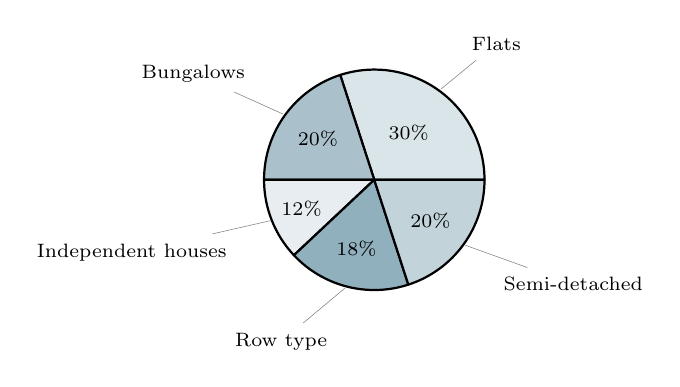
\begin{tikzpicture}\pie[radius=1.4,text=pin,font=\scriptsize,color={brand!15,brand!35,brand!10,brand!45,brand!25}]{30/Flats,20/Bungalows,12/Independent houses,18/Row type,20/Semi-detached}\end{tikzpicture}
\end{center}
\end{context}
\begin{question}{52}
{The 20\% of the total bungalows are white in colour. How many are there?\par}
\optsfour{10}{8}{6}{12}
\answer{C}{6}
\begin{explain}
Bungalows $=20\%$ of $150=30$; white $=20\%$ of $30=\mathbf{6}$.
\end{explain}
\end{question}

\begin{question}{53}
{How many residences are flat type ?\par}
\optsfour{20}{30}{35}{45}
\answer{D}{45}
\begin{explain}
Flats $=30\%$ of $150=\mathbf{45}$.
\end{explain}
\end{question}

\begin{question}{54}
{From among the 12\% independent houses, 50\% are facing east direction. How many are they?\par}
\optsfour{12}{9}{6}{10}
\answer{B}{9}
\begin{explain}
Independent houses $=12\%$ of $150=18$; facing east $=50\%$ of $18=\mathbf{9}$.
\end{explain}
\end{question}

\begin{question}{55}
{In the following if the smallest circle represents candidates clearing GSET exam, bigger circle represents candidates clearing only Paper-I of the GSET exam and the biggest circle represents the candidates who failed in the GSET exam, then choose the diagram which correctly represents this relationships.\par}
\optsfour{\tikz[baseline=-0.5ex,scale=0.3]{\draw (0,0) circle(1.1); \draw (0,0) circle(0.75); \draw (2.2,0) circle(0.6);}}{\tikz[baseline=-0.5ex,scale=0.3]{\draw (0,0) circle(1); \draw (2.2,0) circle(0.8); \draw (3.8,0) circle(0.45);}}{\tikz[baseline=-0.5ex,scale=0.3]{\draw (0,0) circle(1.1); \draw (2.4,0) circle(0.8); \draw (2.4,0) circle(0.4);}}{\tikz[baseline=-0.5ex,scale=0.3]{\draw (0,0) circle(1.2); \draw (0,0) circle(0.85); \draw (0,0) circle(0.5);}}
\answer{A}{\tikz[baseline=-0.5ex,scale=0.3]{\draw (0,0) circle(1.1); \draw (0,0) circle(0.75); \draw (2.2,0) circle(0.6);}}
\begin{explain}
Per the key, (A) is correct. Candidates who clear GSET have necessarily cleared Paper I, so the \textbf{smallest circle lies inside the bigger circle}. Candidates who \textbf{failed} form a separate group, the \textbf{biggest circle, disjoint} from both.
\end{explain}
\end{question}

\begin{question}{56}
{Consider the following statement followed by two assumptions (i) and (ii). Choose the correct answer.\\
\textbf{Statement:} ``You are hereby appointed as a programmer with a probation period of one year and your performance will be reviewed at the end of the period for confirmation.'' --- A line in an appointment letter.\\
\textbf{Assumptions:}\\
(i) The performance of an individual is generally not known at the time of appointment offer.\\
(ii) Generally an individual tries to prove his/her worth in the probation period.\par}
\optsone{Only Assumption (i) is implicit.}{Only Assumption (ii) is implicit.}{None of the assumptions (i) and (ii) are implicit.}{Both the Assumptions (i) and (ii) are implicit.}
\answer{D}{Both the Assumptions (i) and (ii) are implicit.}
\begin{explain}
A probation period is used \emph{because} an appointee's real performance is not known at the time of appointment (i), and because people generally try to prove their worth during probation (ii). \textbf{Both} assumptions are implicit.
\end{explain}
\end{question}

\begin{question}{57}
{Of the following statements, there are two statements both of which cannot be false but both can be true. Which are these two statements?\\
(i) All the students wish to complete their study.\\
(ii) Some students do not like Mathematics.\\
(iii) No student wishes to complete the study.\\
(iv) No student likes Mathematics.\par}
\optsfour{(i) and (ii)}{(iii) and (iv)}{(i) and (iii)}{(ii) and (iv)}
\answer{A}{(i) and (ii)}
\begin{explain}
The official key gives \textbf{(i) and (ii)}. The pair ``All students wish to complete their study'' and ``Some students do not like Mathematics'' can obviously both be true together, and the setters treat them as the pair that cannot both be false.
\tip{In formal logic, two propositions that cannot both be false but can both be true are \emph{sub-contraries} (``Some S are P'' and ``Some S are not P'').}
\end{explain}
\end{question}

\begin{question}{58}
{Evaluate the following statements in terms of whether each is a Fact, Opinion, Prejudice or Advice by choosing correct alternative.\\
(i) Women are not suitable for police service.\\
(ii) In democracy no party should be in power for too long.\\
(iii) Have proper rest even during examination time.\\
(iv) Obesity is a risk factor for coronary heart diseases.\\
Options list the statements in the order: \textbf{Opinion -- Prejudice -- Fact -- Advice}.\par}
\optstwo{(ii) (iii) (iv) (i)}{(ii) (i) (iv) (iii)}{(iii) (i) (iv) (ii)}{(ii) (iv) (iii) (i)}
\answer{B}{(ii) (i) (iv) (iii)}
\begin{explain}
(ii) is an \textbf{opinion}; (i) is a \textbf{prejudice} (a biased generalisation about women); (iv) is a scientific \textbf{fact}; (iii) is \textbf{advice}. The order is (ii), (i), (iv), (iii), which is option (B).
\end{explain}
\end{question}

\begin{question}{59}
{The question below is followed by two arguments numbered (i) and (ii). Decide which argument is strong.\\
\textbf{Question:} Should India encourage exports when most things are insufficient for internal use itself?\\
\textbf{Arguments:}\\
(i) Yes. We have to earn foreign exchange to pay at least for our defence and other necessary imports.\\
(ii) No. Even selective encouragement will lead to shortages.\par}
\optsone{Only Argument (i) is strong.}{Only Argument (ii) is strong.}{Both the Arguments (i) and (ii) are strong.}{None of the arguments (i) and (ii) are strong.}
\answer{A}{Only Argument (i) is strong.}
\begin{explain}
(i) is \textbf{strong}: foreign exchange is essential for necessary imports such as defence equipment and oil. (ii) is weak: it assumes, without basis, that \emph{any} selective export will cause shortages.
\end{explain}
\end{question}

\begin{question}{60}
{Consider the following two statements and choose the correct answer.\\
\textbf{Statement (i):} There has been a high increase in the incidents of atrocities against women in the country during past few years.\\
\textbf{Statement (ii):} The police authority has been unable to nab the culprits committing crime against women.\par}
\optsone{Statement (i) is cause and Statement (ii) is effect.}{Statement (ii) is cause and Statement (i) is effect.}{Statements (i) and (ii) are both independent of causes.}{Statements (i) and (ii) are both effects of some independent causes.}
\answer{C}{Statements (i) and (ii) are both independent of causes.}
\begin{explain}
The official key treats the two statements as \textbf{independent} of each other: the rise in crime has many social causes, and police failure is a separate issue. Neither is shown to cause the other.
\end{explain}
\end{question}

\paperchapter{October 2011}{October 2011}{A}{60}{GSET 2011}
\keytable{\kcell{1}{C} & \kcell{2}{D} & \kcell{3}{C} & \kcell{4}{A} & \kcell{5}{A} & \kcell{6}{C} & \kcell{7}{C} & \kcell{8}{B} & \kcell{9}{B} & \kcell{10}{C} \\
\kcell{11}{D} & \kcell{12}{C} & \kcell{13}{A} & \kcell{14}{C} & \kcell{15}{A} & \kcell{16}{A} & \kcell{17}{D} & \kcell{18}{B} & \kcell{19}{C} & \kcell{20}{C} \\
\kcell{21}{C} & \kcell{22}{C} & \kcell{23}{A} & \kcell{24}{A} & \kcell{25}{D} & \kcell{26}{C} & \kcell{27}{A} & \kcell{28}{D} & \kcell{29}{C} & \kcell{30}{B} \\
\kcell{31}{B} & \kcell{32}{C} & \kcell{33}{D} & \kcell{34}{C} & \kcell{35}{C} & \kcell{36}{C} & \kcell{37}{C} & \kcell{38}{B} & \kcell{39}{D} & \kcell{40}{A} \\
\kcell{41}{B} & \kcell{42}{B} & \kcell{43}{A} & \kcell{44}{B} & \kcell{45}{C} & \kcell{46}{C} & \kcell{47}{B} & \kcell{48}{A} & \kcell{49}{B} & \kcell{50}{B} \\
\kcell{51}{A} & \kcell{52}{B} & \kcell{53}{D} & \kcell{54}{A} & \kcell{55}{C} & \kcell{56}{A} & \kcell{57}{C} & \kcell{58}{C} & \kcell{59}{B} & \kcell{60}{D}}
\begin{context}
\textbf{Read the following text and answer the Question Nos.~1 to 6.}\par\smallskip
The algorithmic theory of beauty takes the subjectivity of the observer into account and postulates that among several observations classified as comparable by a given subjective observer, the aesthetically most pleasing one is the one with the shortest description. This is closely related to the principles of algorithmic information theory and minimum description length. For example, mathematicians welcome simple proof with a short description in their formal language. Another concrete example describes an aesthetically pleasing human face whose proportions can be described by very few bits of information, drawing inspiration from 15th century proportion studies by Leonardo da Vinci. Going further, this theory explicitly distinguishes between what is beautiful and what is interesting. Interestingness corresponds to the first derivative of subjectively perceived beauty. Here, the premise is that any observer continually tries to improve the predictability of the observations by discovering regularities such as repetition and symmetry.
\end{context}
\begin{question}{1}
{According to the algorithmic theory:\par}
\optsone{subjective perceptions of observers' cannot be systematically classified}{there is no correlation between subjective observation and beauty}{there is a positive correlation between beauty and minimum description}{perception of beauty is unpredictable}
\answer{C}{there is a positive correlation between beauty and minimum description}
\begin{explain}
The theory says the most pleasing observation is the one with the \textbf{shortest description}. Beauty therefore increases as description length decreases: there is a \textbf{positive correlation between beauty and minimum description}.
\end{explain}
\end{question}

\begin{question}{2}
{The formal language of mathematics\par}
\optsone{prefers simple proof which may or may not be elaborate}{prefers the least elaborate description and repetition}{may be complex even as it provides a short description}{ensures simplicity and bravity}
\answer{D}{ensures simplicity and bravity}
\begin{explain}
Mathematicians ``welcome simple proof with a short description in their formal language''. The formal language of mathematics therefore values \textbf{simplicity and brevity}.
\end{explain}
\end{question}

\begin{question}{3}
{The author of the passage suggests that Leonardo da Vinci:\par}
\optsone{was a precursor of the algorithmic theory of information}{predicted the algorithmic theory of beauty}{produced proportion studies that support algorithmic theory of beauty}{gave a theory of subjectively perceived aesthetics}
\answer{C}{produced proportion studies that support algorithmic theory of beauty}
\begin{explain}
The passage says the face example draws ``inspiration from 15th century \textbf{proportion studies} by Leonardo da Vinci''. His studies \emph{support} the theory; he did not predict it.
\end{explain}
\end{question}

\begin{question}{4}
{Which of the following is not true ?\par}
\optsone{What is interesting is not always beautiful}{We perceive beauty when we discover symmetry}{Mathematicians prefer short descriptions}{We can distinguish between what is interesting and what is beautiful}
\answer{A}{What is interesting is not always beautiful}
\begin{explain}
The official key marks (A) as the statement not supported. The passage says only that the theory \emph{distinguishes} the interesting from the beautiful, with interestingness being the \emph{rate of change} (first derivative) of perceived beauty. It does not claim that what is interesting is not beautiful.
\end{explain}
\end{question}

\begin{question}{5}
{How do we perceive beauty ?\par}
\optstwo{By noticing patterns of similarity}{By subjective observation}{By identifying a pleasing human face}{By producing the shortest description}
\answer{A}{By noticing patterns of similarity}
\begin{explain}
The observer improves predictability ``by discovering regularities such as \textbf{repetition and symmetry}'', i.e.\ by noticing patterns of similarity.
\end{explain}
\end{question}

\begin{question}{6}
{An appropriate title for the passage would be :\par}
\optstwo{Leonardo da Vinci on Beauty}{Aesthetics and Mathematics}{Algorithmic theory of Beauty}{The Beautiful and the Interesting}
\answer{C}{Algorithmic theory of Beauty}
\begin{explain}
The passage is entirely about the \textbf{algorithmic theory of beauty}.
\end{explain}
\end{question}

\begin{question}{7}
{The gas leaked during Bhopal disaster was:\par}
\optstwo{ethyl cyanoacetate}{ethyl cyanoacrylate}{methyl isocyanate}{methyl diisocyanate}
\answer{C}{methyl isocyanate}
\begin{explain}
The Bhopal gas tragedy (2--3 December 1984, Union Carbide plant) released \textbf{methyl isocyanate (MIC)}, killing thousands. It is the world's worst industrial disaster.
\end{explain}
\end{question}

\begin{question}{8}
{The audible range of frequency for human ear is\par}
\optstwo{10 Hz to 10 kHz}{20 Hz to 20 kHz}{10 Hz to 20 kHz}{10 Hz to 30 kHz}
\answer{B}{20 Hz to 20 kHz}
\begin{explain}
The human audible range is about \textbf{20 Hz to 20 kHz}. Below it is infrasound; above it is ultrasound.
\end{explain}
\end{question}

\begin{question}{9}
{If waste materials contaminate the source of drinking water, which of the following diseases will spread?\par}
\optsfour{Scurvy}{Typhoid}{Malaria}{Anaemia}
\answer{B}{Typhoid}
\begin{explain}
Contaminated drinking water spreads water-borne diseases such as \textbf{typhoid}, cholera and hepatitis A.
\why{Scurvy is vitamin-C deficiency; malaria is mosquito-borne; anaemia is a nutritional deficiency.}
\end{explain}
\end{question}

\begin{question}{10}
{Which of the following is most likely to limit primary production in fresh water lakes?\par}
\optsfour{Oxygen}{Calcium}{Phosphorus}{Carbon}
\answer{C}{Phosphorus}
\begin{explain}
In fresh-water lakes \textbf{phosphorus} is usually the limiting nutrient for algal (primary) production. Excess phosphate from detergents and fertilisers causes eutrophication.
\end{explain}
\end{question}

\begin{question}{11}
{Which of the following is not a major greenhouse gas?\par}
\optstwo{Carbon dioxide}{Methane}{Water vapour}{Calcium carbonate}
\answer{D}{Calcium carbonate}
\begin{explain}
CO$_2$, methane and water vapour are greenhouse gases. \textbf{Calcium carbonate} is a solid (limestone), not a gas.
\end{explain}
\end{question}

\begin{question}{12}
{Tsunami is caused due to :\par}
\optsone{Giant high tide waves in ocean}{Oceanic bad weather conditions}{Sudden motion of the ocean floor}{Intercontinental collisions in the ocean}
\answer{C}{Sudden motion of the ocean floor}
\begin{explain}
A tsunami is caused by the \textbf{sudden displacement (motion) of the ocean floor}, usually by an undersea earthquake, landslide or volcanic eruption.
\end{explain}
\end{question}

\begin{question}{13}
{The full form of FTP is:\par}
\optstwo{File Transfer Protocol}{File Transfer Program}{File Transfer Property}{File Transfer Problem}
\answer{A}{File Transfer Protocol}
\begin{explain}
\textbf{FTP} is \textbf{File Transfer Protocol}, used to transfer files between computers over a network.
\end{explain}
\end{question}

\begin{question}{14}
{For proper functioning of computers, which of the following is not recommended ?\par}
\optsone{Anti-virus should always be activated}{Always use authorized softwares}{Never connect to internet}{Never allow external data devices on your PC without checking for viruses}
\answer{C}{Never connect to internet}
\begin{explain}
Anti-virus, authorised software and scanning external devices are recommended. \textbf{``Never connect to the internet''} is not a recommendation; the internet is essential, and safe use is what matters.
\end{explain}
\end{question}

\begin{question}{15}
{If '10110110' is written on a paper, what does it mean?\par}
\optsfour{Data}{Information}{Knowledge}{Wisdom}
\answer{A}{Data}
\begin{explain}
A bare string of bits such as 10110110, without context or processing, is \textbf{data}.
\tip{DIKW hierarchy: Data $\rightarrow$ Information $\rightarrow$ Knowledge $\rightarrow$ Wisdom.}
\end{explain}
\end{question}

\begin{question}{16}
{Which of the following is not a characteristic of information ?\par}
\optstwo{It is unchangeable with time}{It is meaningful to the receiver}{It is relevant to the activity}{It is clear and concise}
\answer{A}{It is unchangeable with time}
\begin{explain}
Information is meaningful, relevant, clear and \textbf{timely}. Its value \emph{changes with time}, so ``unchangeable with time'' is not a characteristic of information.
\end{explain}
\end{question}

\begin{question}{17}
{The selection of information and communication technological tools should essentially depend on:\par}
\optstwo{Technological infrastructure}{Learner's access to the technology}{The support personnel}{All of the above}
\answer{D}{All of the above}
\begin{explain}
The choice of ICT tools depends on the available infrastructure, learners' access and support staff, i.e.\ \textbf{all of the above}.
\end{explain}
\end{question}

\begin{question}{18}
{Which of the following is a soft copy output device ?\par}
\optstwo{Printer}{Visual Display Unit (VDU)}{CD-ROM}{Both (A) and (B) of the above}
\answer{B}{Visual Display Unit (VDU)}
\begin{explain}
A \textbf{soft copy} is displayed electronically, not printed. The \textbf{VDU (monitor)} is a soft-copy output device; a printer gives hard copy; a CD-ROM is a storage medium.
\end{explain}
\end{question}

\begin{question}{19}
{Which of the following is correct sequence of steps in scientific method?\par}
\optsone{Observation, Deduction of consequences, Hypothesizing, Verification}{Verification, Hypothesizing, Observation, Deduction of consequences}{Observation, Hypothesizing, Deduction of consequences, Verification}{Hypothesizing, Observation, Verification, Deduction of consequences}
\answer{C}{Observation, Hypothesizing, Deduction of consequences, Verification}
\begin{explain}
Scientific method: \textbf{observation $\rightarrow$ hypothesis $\rightarrow$ deduction of consequences $\rightarrow$ verification}.
\end{explain}
\end{question}

\begin{question}{20}
{A research carried out by a practitioner is called:\par}
\optstwo{Applied Research}{Basic Research}{Action Research}{Experimental Research}
\answer{C}{Action Research}
\begin{explain}
Research by a practitioner (teacher, manager) to improve his or her own practice is \textbf{action research}.
\end{explain}
\end{question}

\begin{question}{21}
{Sampling procedure in which every subject of a population has equal chance of being selected is called:\par}
\optstwo{Purposive sampling}{Cluster sampling}{Probability sampling}{Non-probability sampling}
\answer{C}{Probability sampling}
\begin{explain}
When every unit has an equal (known) chance of selection, the procedure is \textbf{probability sampling}.
\end{explain}
\end{question}

\begin{question}{22}
{In research, reliability indicates:\par}
\optstwo{Precision in measurement}{Error in measurement}{Replicability in measurement}{Generalisability in measurement}
\answer{C}{Replicability in measurement}
\begin{explain}
\textbf{Reliability} is the consistency of measurement: the same results on \textbf{replication} (repeated measurement).
\end{explain}
\end{question}

\begin{question}{23}
{An example of non-empirical research is :\par}
\optsfour{Philosophical}{Historical}{Survey}{Experimental}
\answer{A}{Philosophical}
\begin{explain}
\textbf{Philosophical research} relies on reasoning and conceptual analysis rather than empirical data, so it is non-empirical.
\end{explain}
\end{question}

\begin{question}{24}
{Delimitation in research report refers to:\par}
\optsone{Setting limits to the problem of research}{Limitation of the researcher in studying the problem}{Defining the research problem}{Alternative to scope of the problem}
\answer{A}{Setting limits to the problem of research}
\begin{explain}
\textbf{Delimitations} are the boundaries the researcher deliberately sets on the study (population, variables, area, period), i.e.\ \textbf{setting limits to the problem}. \emph{Limitations} are constraints beyond the researcher's control.
\end{explain}
\end{question}

\begin{question}{25}
{The main purpose of classroom teaching is to:\par}
\optsone{prepare students for examination}{make students content expert}{develop competitive spirit among students}{make students apply disciplinary knowledge to life}
\answer{D}{make students apply disciplinary knowledge to life}
\begin{explain}
Classroom teaching aims to help students \textbf{apply disciplinary knowledge to life}, not merely to pass examinations or compete.
\end{explain}
\end{question}

\begin{question}{26}
{Which of the following has potential to influence learning ?\par}
\optstwo{Socio-economic status}{Ability to express}{Study habits}{Ability of books}
\answer{C}{Study habits}
\begin{explain}
Per the key, \textbf{study habits} are the learner factor with the potential to influence learning directly.
\end{explain}
\end{question}

\begin{question}{27}
{Which of the following factors contributes towards effective teaching ?\par}
\optsone{Knowledge of teaching methods and learners}{Knowledge of content and institution}{Knowledge of teaching method and institution}{Knowledge of learner and computer}
\answer{A}{Knowledge of teaching methods and learners}
\begin{explain}
Effective teaching requires \textbf{knowledge of teaching methods and of learners} (pedagogy and psychology), along with content.
\end{explain}
\end{question}

\begin{question}{28}
{Which of the following is the advantage of lecture method ?\par}
\optstwo{Effective face-to-face teaching}{Ensures attention of all students}{Caters to all individual differences}{Suitable for large group teaching}
\answer{D}{Suitable for large group teaching}
\begin{explain}
The lecture method's main advantage is that it is \textbf{suitable for teaching large groups} economically.
\end{explain}
\end{question}

\begin{question}{29}
{Teachers use teaching aids, because:\par}
\optsone{Some teachers are incapable of teaching on their own}{Students require some change while learning}{It is necessary to reach the students' level of understanding}{To use the updated technology of teaching}
\answer{C}{It is necessary to reach the students' level of understanding}
\begin{explain}
Teaching aids are used to reach \textbf{the students' level of understanding}, making ideas concrete and clear.
\end{explain}
\end{question}

\begin{question}{30}
{Internal assessment marks are to be:\par}
\optstwo{kept confidential}{revealed to students}{based on attendance}{used as gracing marks}
\answer{B}{revealed to students}
\begin{explain}
Internal assessment marks should be \textbf{revealed to students} so that they get feedback and the process stays transparent.
\end{explain}
\end{question}

\begin{question}{31}
{Efficacy and effectiveness of communication can be assessed through:\par}
\optsfour{Reception}{Feedback}{Transmission}{Encoding}
\answer{B}{Feedback}
\begin{explain}
The effectiveness of communication is judged by \textbf{feedback}, which shows whether the message was understood as intended.
\end{explain}
\end{question}

\begin{question}{32}
{Which one of the following aspects has no influence in face-to-face communication ?\par}
\optstwo{Language ability}{Facial expressions}{Location}{Acquaintance}
\answer{C}{Location}
\begin{explain}
Language, facial expressions and acquaintance all influence face-to-face communication. The key treats \textbf{location} as having no influence.
\end{explain}
\end{question}

\begin{question}{33}
{Which of the following is not a type of communication ?\par}
\optstwo{Vertical communication}{Horizontal communication}{Crosswise communication}{Verbal communication}
\answer{D}{Verbal communication}
\begin{explain}
Vertical, horizontal and crosswise (diagonal) are the \emph{directions} of communication flow in an organisation. The key gives \textbf{verbal communication} as the answer: it is classified by \emph{mode}, not by direction, so it does not belong to this set of types.
\end{explain}
\end{question}

\begin{question}{34}
{Noise in communication is to:\par}
\optstwo{Block the media}{Distort the message codes}{Add on the message codes}{Distort the decoding}
\answer{C}{Add on the message codes}
\begin{explain}
Per the key, noise \textbf{adds on to the message codes}: unwanted signals get added to the message and distort it.
\end{explain}
\end{question}

\begin{question}{35}
{Which of the following is a pre-requisite for effective classroom communication ?\par}
\optstwo{Reflective questioning}{Elaborate explanation}{Drawing attention of students}{Planning the lesson}
\answer{C}{Drawing attention of students}
\begin{explain}
The first requirement for classroom communication is \textbf{drawing the students' attention}. Without attention no message is received.
\end{explain}
\end{question}

\begin{question}{36}
{Which of the following is not a feedback loop in classroom communication?\par}
\optstwo{Answering a question}{Taking down the notes}{Creating disturbance}{Cross-questioning the teacher}
\answer{C}{Creating disturbance}
\begin{explain}
Answering questions, taking notes and cross-questioning the teacher are responses that feed back to the teacher. \textbf{Creating disturbance} is not a feedback loop in classroom communication.
\end{explain}
\end{question}

\begin{question}{37}
{Participation of students representatives in higher education governing bodies is advisable to:\par}
\optsone{treat students community at par with teacher}{prepare future politicians}{promote democratic citizenship}{provide extra privilege to subside student unrest}
\answer{C}{promote democratic citizenship}
\begin{explain}
Student representation in governing bodies helps \textbf{promote democratic citizenship}: participation, responsibility and a voice in decisions.
\end{explain}
\end{question}

\begin{question}{38}
{Researches in the area of environmental education fall under:\par}
\optstwo{Inter-disciplinary research}{Multi-disciplinary research}{Intra-disciplinary research}{Uni-disciplinary research}
\answer{B}{Multi-disciplinary research}
\begin{explain}
Environmental education draws on biology, chemistry, geography, economics and sociology, so it is \textbf{multi-disciplinary} research.
\end{explain}
\end{question}

\begin{question}{39}
{The purpose of distance education in India is to:\par}
\optstwo{provide degrees economically}{generate large number of graduates}{increase the rate of higher education}{reach the unreachables}
\answer{D}{reach the unreachables}
\begin{explain}
Distance education aims to \textbf{reach the unreached}: people who cannot attend regular institutions because of distance, work or circumstances.
\end{explain}
\end{question}

\begin{question}{40}
{Teaching at higher education is:\par}
\optstwo{not a job, though salaried}{not a time based activity}{not a contractual activity}{not a cost effective activity}
\answer{A}{not a job, though salaried}
\begin{explain}
Teaching in higher education is a vocation and mission: it is \textbf{not merely a job, though salaried}.
\end{explain}
\end{question}

\begin{question}{41}
{How can teacher inculcate values among students ?\par}
\optsone{By imposing discipline}{By behaving ideally}{By telling life histories of great people}{By telling moral stories}
\answer{B}{By behaving ideally}
\begin{explain}
Values are best taught by example: the teacher must \textbf{behave ideally} (``values are caught, not taught'').
\end{explain}
\end{question}

\begin{question}{42}
{Educational institutes' accrediting bodies are:\par}
\optsone{Government bodies to control and regulate Government policies}{Statutory bodies to maintain quality of education}{Bodies to control management indulging in large profits}{Bodies to improve examination system of educational institution}
\answer{B}{Statutory bodies to maintain quality of education}
\begin{explain}
Accrediting bodies (NAAC, NBA) are \textbf{statutory or autonomous bodies to maintain and assure the quality of education}.
\end{explain}
\end{question}

\begin{question}{43}
{Complete the sequence of squares by choosing the correct figure from the given alternatives:\\[3pt]
\centering
\newcommand{\sq}[1]{\framebox[1.1cm][c]{\rule{0pt}{0.8cm}\parbox[c]{1cm}{\centering\tiny #1}}}
\sq{$\angle$}\,\sq{$\triangle\angle$}\,\sq{$\triangle\triangle\triangle$}\,\sq{$\triangle\triangle\triangle$\\$\triangle\angle$}\,\sq{$\triangle\triangle\triangle$\\$\triangle\triangle\triangle$\\$\angle$}\,\sq{?}\par}
\optsfour{\framebox{\parbox{0.9cm}{\centering\tiny$\triangle\triangle\triangle$\\$\triangle\triangle\triangle$\\$\triangle\triangle\triangle$}}}{\framebox{\parbox{0.9cm}{\centering\tiny$\triangle\triangle\triangle$\\$\triangle\triangle\triangle$\\$\triangle\triangle\triangle$\\$\triangle\angle$}}}{\framebox{\parbox{0.9cm}{\centering\tiny$\triangle\triangle\triangle$\\$\triangle\triangle\triangle$\\$\triangle\triangle\triangle$\\$\triangle\triangle\angle$}}}{\framebox{\parbox{0.9cm}{\centering\tiny$\triangle\triangle\triangle$\\$\triangle\triangle\triangle$\\$\triangle\angle\angle$}}}
\answer{A}{\framebox{\parbox{0.9cm}{\centering\tiny$\triangle\triangle\triangle$\\$\triangle\triangle\triangle$\\$\triangle\triangle\triangle$}}}
\begin{explain}
The number of complete triangles grows $0, 1, 3, 4, 6, \ldots$ and the figure alternates between having a half-drawn triangle ($\angle$) and not having one. In the 3rd figure the angle is ``completed'' into a full row of triangles; likewise the next step completes the figure into \textbf{three full rows, i.e.\ nine triangles}, as in option (A).
\end{explain}
\end{question}

\begin{question}{44}
{Put the correct letter for `?' in the following diagram:\\[3pt]
\centering\begin{tabular}{ccc}
\framebox{C} & $\triangleright$ B & \textcircled{F}\\[2pt]
\framebox{D} & $\triangleright$ C & \textcircled{?}\\[2pt]
\framebox{E} & $\triangleright$ D & \textcircled{T}\\
\end{tabular}\par}
\optsfour{H}{L}{M}{P}
\answer{B}{L}
\begin{explain}
The circle letter's position is the \textbf{product} of the other two positions:
\[\text{C}(3)\times\text{B}(2)=6=\text{F},\qquad \text{E}(5)\times\text{D}(4)=20=\text{T}\]
\[\text{D}(4)\times\text{C}(3)=12=\mathbf{L}\]
\end{explain}
\end{question}

\begin{question}{45}
{Take Universal set U $=\{$A, B, C, \ldots, Z$\}$ of all English alphabets. If set A contains the letters from GUJARAT, the members of set B are the alphabets from PUNJAB, the set C contains the alphabets from SIKKIM and the elements of the set D are the alphabets from TAMILNADU, then the Venn diagram for the sets A, B, C, D will be:\par}
\optsfour{\tikz[baseline=-0.5ex,scale=0.25]{\draw (-2,-2) rectangle (2,2); \draw (0,0.8) circle(0.8); \draw (-0.8,0) circle(0.8); \draw (0.8,0) circle(0.8); \draw (0,-0.8) circle(0.8);}}{\tikz[baseline=-0.5ex,scale=0.25]{\draw (-2,-2) rectangle (2,2); \draw (-0.6,1.1) circle(0.7); \draw (-0.6,0) circle(0.7); \draw (-0.6,-1.1) circle(0.7); \draw (0.7,0.1) circle(0.7);}}{\tikz[baseline=-0.5ex,scale=0.25]{\draw (-2,-2) rectangle (2,2); \draw (-0.9,-0.5) circle(0.7); \draw (0.1,0) circle(0.7); \draw (0.8,0.6) circle(0.7); \draw (0.7,-0.2) circle(0.7);}}{\tikz[baseline=-0.5ex,scale=0.25]{\draw (-2,-2) rectangle (2,2); \draw (0,0.8) circle(0.9); \draw (-0.2,1.0) circle(0.35); \draw (0,-0.8) circle(0.9); \draw (-0.2,-1.1) circle(0.35);}}
\answer{C}{\tikz[baseline=-0.5ex,scale=0.25]{\draw (-2,-2) rectangle (2,2); \draw (-0.9,-0.5) circle(0.7); \draw (0.1,0) circle(0.7); \draw (0.8,0.6) circle(0.7); \draw (0.7,-0.2) circle(0.7);}}
\begin{explain}
Write out the sets:
\begin{center}\small
\begin{tabular}{ll}
A (GUJARAT) & \{G, U, J, A, R, T\}\\ B (PUNJAB) & \{P, U, N, J, A, B\}\\ C (SIKKIM) & \{S, I, K, M\}\\ D (TAMILNADU) & \{T, A, M, I, L, N, D, U\}\\
\end{tabular}
\end{center}
A$\cap$B $=$ \{U, J, A\}, A$\cap$D $=$ \{T, A, U\}, B$\cap$D $=$ \{U, N, A\}, and A$\cap$B$\cap$D $=$ \{U, A\}. C shares \{I, M\} with D only and nothing with A or B.
So A, B, D overlap mutually and C overlaps only D, as in diagram \textbf{(C)}.
\end{explain}
\end{question}

\begin{question}{46}
{A fighter pilot notices a row of several tanks of enemy. He attacks on the tank T at the middle in the row. He then attacks on one more tank T1 in that row immediately preceding to T. In order to finish the last tank in that row, he has to attack 9th tank counting in order from T1. The total number of tanks in that row is:\par}
\optsfour{13}{11}{17}{15}
\answer{C}{17}
\begin{explain}
T is the middle tank and T1 is the tank immediately before it. From T1 the pilot counts 9 more tanks to reach the last one, so there are $9-1=8$ tanks after T. Since T is in the middle, there are also 8 tanks before T.
Total $=8+1+8=\mathbf{17}$.
\end{explain}
\end{question}

\begin{question}{47}
{Fill in the cell of `?' by putting the correct letter:\\[3pt]
\centering\begin{tabular}{|c|c|c|}\hline G & B & C\\\hline H & F & H\\\hline A & D & ?\\\hline\end{tabular}\par}
\optsfour{G}{E}{P}{N}
\answer{B}{E}
\begin{explain}
Per the key the answer is \textbf{E}. With letter positions, the first and third columns then have the same total, $G+H+A=7+8+1=16=C+H+E=3+8+5$, balancing about the middle column.
\end{explain}
\end{question}

\begin{question}{48}
{Which member of the following set differs from the other members ? (OX, GIRAFFE, CAMEL, DOG, GOAT, ELEPHANT, DEER)\par}
\optsfour{DOG}{DEER}{CAMEL}{OX}
\answer{A}{DOG}
\begin{explain}
Ox, giraffe, camel, goat, elephant and deer are \textbf{herbivores}; the \textbf{dog} is a carnivore (and a pet), so it is the odd one out.
\end{explain}
\end{question}

\begin{question}{49}
{Put the number in the empty box by choosing the correct digit from the given alternatives:\\[3pt]
\centering\begin{tabular}{|c|c|c|}\hline 7 & 3 & 6\\\hline 5 & 4 & 7\\\hline 8 & ? & 2\\\hline\end{tabular}\par}
\optsfour{9}{6}{5}{3}
\answer{B}{6}
\begin{explain}
Each row adds up to 16: $7+3+6=16$ and $5+4+7=16$, so $8+?+2=16$ gives $?=\mathbf{6}$.
\end{explain}
\end{question}

\begin{question}{50}
{If $a*b=\dfrac{b}{a}$, then which of the following statements is \emph{not} true? ($a$ and $b$ are real numbers)\par}
\optsfour{$a*0=0,\ a\neq0$}{$0*b=0,\ b\neq0$}{$1*1=1$}{$a*a=1,\ a\neq0$}
\answer{B}{$0*b=0,\ b\neq0$}
\begin{explain}
$0*b=\dfrac{b}{0}$ is \textbf{undefined} (division by zero), so (B) is not true.
Check the others: $a*0=0/a=0$ \checkmark; $1*1=1$ \checkmark; $a*a=a/a=1$ \checkmark.
\end{explain}
\end{question}

\begin{question}{51}
{For which set of values of $p, q, P, Q$ and for which arithmetic operation $*$, the expression $\left(\dfrac{p}{P}\right)*\left(\dfrac{q}{Q}\right)=-1$?\par}
\optstwo{p = -1, q = 5, P = Q = -4 and * is '+'}{p = P = 1, q = Q = -1 and * is 'x'}{p = Q = -1, q = P = 1 and * is '-'}{p = q = P = 1, Q = -1 and * is '/'}
\answer{A}{p = -1, q = 5, P = Q = -4 and * is '+'}
\begin{explain}
Option (A): $\dfrac{-1}{-4}+\dfrac{5}{-4}=\dfrac14-\dfrac54=-1$ \checkmark.
(B) gives $1\times1=1$; (C) gives $-1\div-1=1$; (D) gives $1-(-1)=2$.
\end{explain}
\end{question}

\begin{question}{52}
{Complete the sequence by putting the appropriate number from the given alternatives: 12, 15, 16, 20, 20, 25, 24, ?\par}
\optsfour{24}{30}{27}{35}
\answer{B}{30}
\begin{explain}
Two interleaved series: $12, 16, 20, 24$ ($+4$) and $15, 20, 25, \mathbf{30}$ ($+5$).
\end{explain}
\end{question}

\begin{question}{53}
{What is the appropriate missing letter in the following sequence ? A, B, D, H, ?\par}
\optsfour{I}{L}{M}{P}
\answer{D}{P}
\begin{explain}
Positions double: A(1), B(2), D(4), H(8), \textbf{P(16)}.
\end{explain}
\end{question}

\begin{question}{54}
{If $l=\sqrt3$, $m=1/7$, $n=2$ and $t=5/4$, then $l^2 * m \;\square\; n \;o\; t=-11/28$ for\par}
\optstwo{$*$, $\square$ and $o$ are all `$-$'}{$*$ is $+$, $\square$ is $+$, $o$ is `$-$'}{$*$ is $-$, $\square$ is $-$, $o$ is `$+$'}{$*$, $\square$ and $o$ are all `$+$'}
\answer{A}{$*$, $\square$ and $o$ are all `$-$'}
\begin{explain}
With all three operations as minus: $3-\dfrac17-2-\dfrac54=\dfrac{84-4-56-35}{28}=-\dfrac{11}{28}$ \checkmark.
\end{explain}
\end{question}

\begin{context}
Answer the questions 55, 56 and 57 from the given data in graphical form. Given data of number of washing machines in thousands, manufactured by two companies A and B, during 1997 to 2002.
\begin{center}
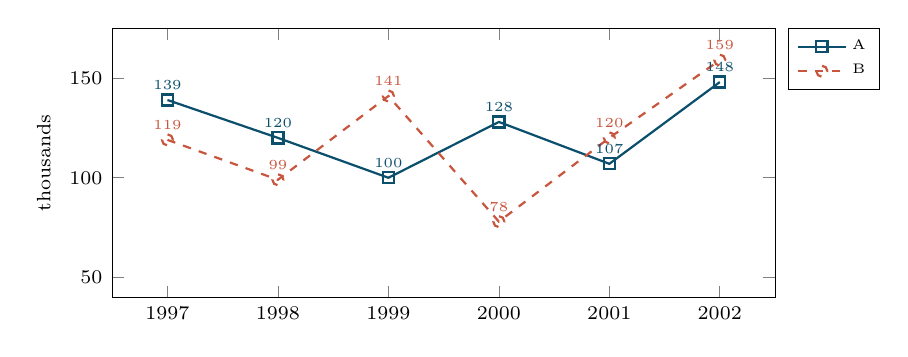
\begin{tikzpicture}
\begin{axis}[width=10cm,height=5cm,xmin=1996.5,xmax=2002.5,ymin=40,ymax=175,xtick={1997,...,2002},
  x tick label style={/pgf/number format/1000 sep=},tick label style={font=\scriptsize},ylabel={\scriptsize thousands},
  nodes near coords,every node near coord/.append style={font=\tiny},legend style={font=\tiny,at={(1.02,1)},anchor=north west}]
\addplot[mark=square,thick,brand] coordinates {(1997,139) (1998,120) (1999,100) (2000,128) (2001,107) (2002,148)};
\addplot[mark=o,thick,dashed,accent] coordinates {(1997,119) (1998,99) (1999,141) (2000,78) (2001,120) (2002,159)};
\legend{A,B}
\end{axis}
\end{tikzpicture}
\end{center}
\end{context}
\begin{question}{55}
{What is the difference between the number of washing machines manufactured by company B in 1997 and 1998?\par}
\optsfour{10,000}{11,000}{20,000}{30,000}
\answer{C}{20,000}
\begin{explain}
B: $119-99=20$ thousand $=\mathbf{20{,}000}$.
\end{explain}
\end{question}

\begin{question}{56}
{What is approximate average number of washing machines manufactured by company A over the given period?\par}
\optsfour{123666}{741999}{431555}{310111}
\answer{A}{123666}
\begin{explain}
A: $\dfrac{139+120+100+128+107+148}{6}=\dfrac{742}{6}\approx123.67$ thousand $\approx\mathbf{123666}$.
\end{explain}
\end{question}

\begin{question}{57}
{In which year the difference between the production of companies A and B was minimum?\par}
\optsfour{1997}{1998}{2002}{2001}
\answer{C}{2002}
\begin{explain}
Differences (thousand): 1997: 20; 1998: 21; 1999: 41; 2000: 50; 2001: 13; 2002: \textbf{11}. The minimum is in \textbf{2002}.
\end{explain}
\end{question}

\begin{context}
Given the table of marks obtained by two candidates P and Q in four papers. Answer the following questions 58, 59 and 60 from this data.
\begin{center}\small
\begin{tabular}{lcccc}\toprule \textbf{Paper} & I & II & III & IV\\\midrule
Maximum marks & 80 & 70 & 100 & 60\\ Candidate P & 48 & 56 & 75 & 42\\ Candidate Q & 40 & 63 & 82 & 36\\\bottomrule
\end{tabular}
\end{center}
\end{context}
\begin{question}{58}
{Arrange in increasing order the \% marks obtained by the candidate P. The sequence of papers is:\par}
\optsfour{I, II, IV, III}{I, III, II, IV}{I, IV, III, II}{II, III, I, IV}
\answer{C}{I, IV, III, II}
\begin{explain}
P's percentages: I $=48/80=60\%$, II $=56/70=80\%$, III $=75\%$, IV $=42/60=70\%$.
Increasing order: \textbf{I (60), IV (70), III (75), II (80)}.
\end{explain}
\end{question}

\begin{question}{59}
{In which paper(s) the candidate Q obtained the distinction?\par}
\optsfour{III}{II, III}{II, III, IV}{II}
\answer{B}{II, III}
\begin{explain}
Q's percentages: I $=50\%$, II $=63/70=90\%$, III $=82\%$, IV $=60\%$. Distinction ($\ge75\%$) in \textbf{II and III}.
\end{explain}
\end{question}

\begin{question}{60}
{Approximate \% results of candidates P and Q will respectively, be:\par}
\optsfour{70\% and 80\%}{70\% and 60\%}{70\% and 50\%}{71\% and 70\%}
\answer{D}{71\% and 70\%}
\begin{explain}
Both candidates total $221/310$: P $=48+56+75+42=221$ and Q $=40+63+82+36=221$, so each scores about $71.3\%$. Among the options, the key takes \textbf{71\% and 70\%} as the approximate results.
\end{explain}
\end{question}

\paperchapter{October 2010}{October 2010}{A}{60}{GSET 2010}
\keytable{\kcell{1}{C} & \kcell{2}{C} & \kcell{3}{D} & \kcell{4}{D} & \kcell{5}{D} & \kcell{6}{A} & \kcell{7}{B} & \kcell{8}{C} & \kcell{9}{A} & \kcell{10}{C} \\
\kcell{11}{C} & \kcell{12}{D} & \kcell{13}{B} & \kcell{14}{C} & \kcell{15}{B} & \kcell{16}{A} & \kcell{17}{A} & \kcell{18}{B} & \kcell{19}{B} & \kcell{20}{A} \\
\kcell{21}{C} & \kcell{22}{B} & \kcell{23}{A} & \kcell{24}{B} & \kcell{25}{B} & \kcell{26}{B} & \kcell{27}{D} & \kcell{28}{A} & \kcell{29}{D} & \kcell{30}{C} \\
\kcell{31}{A} & \kcell{32}{B} & \kcell{33}{D} & \kcell{34}{C} & \kcell{35}{A} & \kcell{36}{D} & \kcell{37}{A} & \kcell{38}{C} & \kcell{39}{B} & \kcell{40}{D} \\
\kcell{41}{C} & \kcell{42}{B} & \kcell{43}{D} & \kcell{44}{C} & \kcell{45}{C} & \kcell{46}{C} & \kcell{47}{X} & \kcell{48}{D} & \kcell{49}{B} & \kcell{50}{B} \\
\kcell{51}{C} & \kcell{52}{C} & \kcell{53}{D} & \kcell{54}{D} & \kcell{55}{C} & \kcell{56}{B} & \kcell{57}{C} & \kcell{58}{A} & \kcell{59}{D} & \kcell{60}{B}}
\begin{question}{1}
{Which of the following statements defines education best ?\par}
\optstwo{Education is a means of social change}{Education imparts useful knowledge}{It prepares autonomous human beings}{It generates a lot of employment}
\answer{C}{It prepares autonomous human beings}
\begin{explain}
The best definition of education is that it \textbf{prepares autonomous human beings}: individuals who think, judge and act independently and responsibly. Social change, useful knowledge and employment are only by-products.
\end{explain}
\end{question}

\begin{question}{2}
{Semester system is recommended as it is considered to:\par}
\optsone{help students learn more efficiently and be regular}{reduce examination orientedness and increase emphasis on learning}{provide scope for continual appraisal and on course correction in teaching-learning process}{allow for more creative ways of teaching}
\answer{C}{provide scope for continual appraisal and on course correction in teaching-learning process}
\begin{explain}
The semester system provides \textbf{scope for continual appraisal}: frequent assessment, feedback and course correction within shorter learning units, per the official key.
\end{explain}
\end{question}

\begin{question}{3}
{It is said that teachers must enable students to own the responsibility for learning. This means teachers\par}
\optsone{have reduced responsibility of learning}{assign learning tasks to students}{ask students to study on their own}{must help students to evolve one's own ways of learning}
\answer{D}{must help students to evolve one's own ways of learning}
\begin{explain}
Making students own responsibility for learning means the teacher \textbf{helps students evolve their own ways of learning}, so that they become self-directed, independent learners.
\end{explain}
\end{question}

\begin{question}{4}
{At higher education stage emphasis needs to be on, not only 'what' and 'how much' is learned by students but 'how' and 'how well' they learn. This idea is expressed at present as:\par}
\optstwo{Learning to know}{Learning to live}{Learning to do}{Learning to learn}
\answer{D}{Learning to learn}
\begin{explain}
Emphasis on ``how'' and ``how well'' students learn reflects the idea of \textbf{learning to learn}, i.e.\ developing metacognition and lifelong learning skills. (Compare the Delors Report's four pillars: learning to know, to do, to live together, to be.)
\end{explain}
\end{question}

\begin{question}{5}
{The current thinking of assessing students only at the end of the term is less relevant as it :\par}
\optsone{reveals student's learning in respect of subject matter}{concerns with how accurately one recollects the subject matter}{may reveal 'temporary learning' and not beyond}{assesses student learning on 'what is asked' rather than 'what is learned' even beyond subject matter}
\answer{D}{assesses student learning on 'what is asked' rather than 'what is learned' even beyond subject matter}
\begin{explain}
Assessment only at the end of term is less useful because it may capture \textbf{temporary learning} (crammed and soon forgotten) rather than lasting understanding. Continuous assessment gives a truer picture.
\end{explain}
\end{question}

\begin{question}{6}
{Arrange the following from the least difficult to most difficult:\newline (1) Teaching of processes\newline (2) Teaching of values\newline (3) Teaching of concepts\newline (4) Teaching of thinking skills\par}
\optstwo{(1), (3), (4), (2)}{(2), (4), (3), (1)}{(1), (3), (2), (4)}{(1), (2), (3), (4)}
\answer{A}{(1), (3), (4), (2)}
\begin{explain}
From least to most difficult: teaching \textbf{processes (1)} $\rightarrow$ \textbf{concepts (3)} $\rightarrow$ \textbf{thinking skills (4)} $\rightarrow$ \textbf{values (2)}. Values are the hardest because they involve the affective domain and must be internalised.
\end{explain}
\end{question}

\begin{question}{7}
{Recently a separate Board has been established to monitor all \ldots{} education institutions in Gujarat.\par}
\optsfour{legal}{technical}{medical}{professional}
\answer{B}{technical}
\begin{explain}
Gujarat set up a separate board (Admission Committee for Professional Courses / the regulatory board under the Gujarat Professional \textbf{Technical} Educational Colleges or Institutions Act, 2007) to regulate admissions and fees of \textbf{technical} education institutions, per the key.
\end{explain}
\end{question}

\begin{question}{8}
{The increasing number of entrants into higher education has necessitated changes in our views of teaching learning. Some progressive institutions have faced this through the adoption of multimedia for teaching-learning. This means, the use of \ldots{} for teaching learning.\par}
\optsone{lecture-cum-discussion, practical work}{face to face, distance and open learning (ODL) systems}{ODL, face to face, satellite and web based modes}{self-learning, ICT based, ODL}
\answer{C}{ODL, face to face, satellite and web based modes}
\begin{explain}
Progressive institutions cope with rising numbers by using multimedia across \textbf{ODL, face-to-face, satellite and web-based modes}, i.e.\ blended and multi-mode delivery.
\end{explain}
\end{question}

\begin{question}{9}
{Apart from specialisation in one's subject areas, products of higher education are also expected to be \ldots{} in the context of national development.\par}
\optsone{sensitive and proactive towards emerging concerns and issues}{responsible workers in one's institution}{aware of the economic changes especially the job market}{tolerant to the negative forces}
\answer{A}{sensitive and proactive towards emerging concerns and issues}
\begin{explain}
Graduates are expected to be \textbf{sensitive and proactive towards emerging concerns and issues} of society and the nation, not merely job-seekers.
\end{explain}
\end{question}

\begin{question}{10}
{To ensure quality maintenance in universities and colleges guidelines and regulations are periodically prepared by the \ldots{} at the national level.\par}
\optsone{National Assessment and Accreditation Council (NAAC)}{National Council for Educational Research and Training (NCERT)}{University Grants Commission (UGC)}{National Institute of Advanced Study (NIAS)}
\answer{C}{University Grants Commission (UGC)}
\begin{explain}
The \textbf{UGC} frames regulations and guidelines for maintaining standards in universities and colleges (UGC Act, 1956, Section 12). NAAC only assesses and accredits.
\end{explain}
\end{question}

\begin{question}{11}
{The open university at the national level in India is known as:\par}
\optsone{Indian General National Open University}{Integrated Governmental National Open University}{Indira Gandhi National Open University}{Iswarbhai Gordhanbhai National Open University}
\answer{C}{Indira Gandhi National Open University}
\begin{explain}
The national open university is \textbf{Indira Gandhi National Open University (IGNOU)}, New Delhi (1985).
\end{explain}
\end{question}

\begin{question}{12}
{Three kinds of universities in India are:\par}
\optsone{State Universities, Central Universities, Affiliating Universities}{Unitary Universities, Technical Universities, General Education Universities}{State Universities, Central Universities, Private Universities}{Central Universities, State Universities, Deemed Universities}
\answer{D}{Central Universities, State Universities, Deemed Universities}
\begin{explain}
Per the key, the three kinds are \textbf{State Universities, Central Universities and Deemed-to-be Universities} (with private universities being added later).
\end{explain}
\end{question}

\begin{question}{13}
{A condition or characteristic that can take on different values or categories is called:\par}
\optstwo{a constant}{a variable}{a cause and effect relationship}{a descriptive relationship}
\answer{B}{a variable}
\begin{explain}
A characteristic that can take different values or categories is a \textbf{variable}; one that cannot vary is a constant.
\end{explain}
\end{question}

\begin{question}{14}
{A researcher wants to find out the relationship between gender and intelligence among high school students. This would be :\par}
\optstwo{a Case Study}{a Developmental Study}{a Survey Study}{an Experimental Study}
\answer{C}{a Survey Study}
\begin{explain}
Studying the relationship between gender and intelligence in a population of students, as they exist without manipulation, is a \textbf{survey (descriptive--correlational) study}.
\end{explain}
\end{question}

\begin{question}{15}
{The best graphical way to present data related to different levels of a certain variable is:\par}
\optstwo{pictogram}{pie chart}{histogram}{frequency polygon}
\answer{B}{pie chart}
\begin{explain}
Per the key, a \textbf{pie chart} best shows how a whole is divided among the different levels (categories) of a variable.
\end{explain}
\end{question}

\begin{question}{16}
{In simple terms 'reliability' is the:\par}
\optsone{consistency of scores on tests}{appropriateness of interpretation based on test scores}{ways in which people are the same}{rank order of participants on some measure}
\answer{A}{consistency of scores on tests}
\begin{explain}
\textbf{Reliability} is the \textbf{consistency} (stability) of test scores. Appropriateness of interpretations is \emph{validity}.
\end{explain}
\end{question}

\begin{question}{17}
{A researcher was interested in studying why learning of new maths was not effective in schools during 1990s. For this, he interviewed several teachers who had taught new maths at that time. These teachers were \ldots{} for his study.\par}
\optstwo{primary sources}{secondary sources}{external critics}{internal critics}
\answer{A}{primary sources}
\begin{explain}
Teachers who personally taught the new maths are eye-witnesses, so they are \textbf{primary sources}.
\end{explain}
\end{question}

\begin{question}{18}
{A positive correlation is present when:\par}
\optsone{two variables move in opposite directions}{two variables move in the same direction}{both variables have negative values}{several variables rarely change}
\answer{B}{two variables move in the same direction}
\begin{explain}
In a \textbf{positive correlation} both variables move in the \textbf{same direction} (both increase or both decrease).
\end{explain}
\end{question}

\begin{context}
\textbf{Directions (Q.~Nos.~19 to 21):} Given data tabulates admission (in percentage) of the candidates to the four courses in five years from 1991 to 1995.
\begin{center}\small
\begin{tabular}{lcccc}\toprule \textbf{Year} & \textbf{Biology} & \textbf{Geology} & \textbf{Chemistry} & \textbf{Mathematics}\\\midrule
1991 & 35 & 30 & 20 & 15\\ 1992 & 40 & 35 & 15 & 10\\ 1993 & 30 & 25 & 20 & 25\\ 1994 & 20 & 20 & 30 & 30\\ 1995 & 30 & 30 & 25 & 15\\\bottomrule
\end{tabular}
\end{center}
\end{context}
\begin{question}{19}
{What is the \% of increase in number of candidates choosing chemistry from 1993 to 1994?\par}
\optsfour{25}{50}{100}{75}
\answer{B}{50}
\begin{explain}
Chemistry: 1993 $=20\%$, 1994 $=30\%$. Increase $=\dfrac{30-20}{20}\times100=\mathbf{50\%}$.
\end{explain}
\end{question}

\begin{question}{20}
{What is the \% of fall of number of candidates in Biology from 1992 to 1993?\par}
\optsfour{25}{50}{100}{75}
\answer{A}{25}
\begin{explain}
Biology: 1992 $=40\%$, 1993 $=30\%$. Fall $=\dfrac{40-30}{40}\times100=\mathbf{25\%}$.
\end{explain}
\end{question}

\begin{question}{21}
{In which subject the strength (in \%) was least in the year 1993 ?\par}
\optsfour{Biology}{Geology}{Chemistry}{Mathematics}
\answer{C}{Chemistry}
\begin{explain}
1993: Biology 30, Geology 25, \textbf{Chemistry 20}, Mathematics 25. The least is Chemistry.
\end{explain}
\end{question}

\begin{context}
\textbf{Directions (Q.~Nos.~22 to 24):} The following data provides the information of outgoing students from an academic institution after completing their study.
\begin{center}\small
\begin{tabular}{lccc}\toprule \textbf{Percentage of students} & \textbf{2003} & \textbf{2004} & \textbf{2005}\\\midrule
by campus recruitment & 33 & 38 & 39\\ in further study & 40 & 36 & 37\\ unemployed & 2 & 1 & 3\\ to other activities & 25 & 25 & 22\\\midrule
Total number of students & 1200 & 1100 & 1000\\\bottomrule
\end{tabular}
\end{center}
\end{context}
\begin{question}{22}
{What is the largest number of students employed through campus recruitment ?\par}
\optsfour{396}{418}{490}{430}
\answer{B}{418}
\begin{explain}
Campus recruitment: 2003 $=33\%\times1200=396$; 2004 $=38\%\times1100=\mathbf{418}$; 2005 $=39\%\times1000=390$. The largest is 418.
\end{explain}
\end{question}

\begin{question}{23}
{What is decrease in number of students going for further studies during 2003-05?\par}
\optsfour{110}{100}{30}{10}
\answer{A}{110}
\begin{explain}
Further studies: 2003 $=40\%\times1200=480$; 2005 $=37\%\times1000=370$. Decrease $=\mathbf{110}$.
\end{explain}
\end{question}

\begin{question}{24}
{How many students choose other activities in 2004?\par}
\optsfour{300}{275}{220}{200}
\answer{B}{275}
\begin{explain}
Other activities in 2004 $=25\%\times1100=\mathbf{275}$.
\end{explain}
\end{question}

\begin{context}
\textbf{Directions (Q.~Nos.~25 to 30):} Read the following text and answer the questions.\par\smallskip
The world is becoming global rapidly. The national boundaries have become less significant with the interlinked effects of technology, information flows and investment mobility. Human knowledge, particularly in the sphere of science and technology, is now growing at a pace which was indeed unthinkable even two decades ago. The comparative advantage of a nation will be more and more influenced by its capacity to generate, absorb, adapt and assimilate new technologies into production process. If liberalisation and globalisation are not to create islands of prosperity surrounded by vast sea of destitution, there has to be firm commitment to human resource development and to continuous upgrading of human skills and capabilities in the fast changing world that we live in. The Indian policy makers are fully committed to building a society which is technologically sophisticated, economically progressive and socially just and humane.

Impact of globalisation on education is now being felt in India. Indian entrepreneurs are also now investing in education. In the process of privatisation of higher education in India, many good institutions have come up and have met the increasing demand for higher education mainly in the area of engineering, business administration and medical education. But this process has also led to mushroom growth of low quality institutions without proper infrastructure. However, the expansion of higher education in India has resulted in increasing access to higher education even in rural areas of the country. In this process, Human Resource Development is taking place at a faster speed as compared to the earlier stage when the opportunities for higher education were limited.

Globalisation has promoted information technology in India. Indian students have excelled in the area of information technology over many other countries. Developments taking place in the developed countries become available to Indian students, scholars and practitioners through regular contacts and through the modern technology.
\end{context}
\begin{question}{25}
{How has new technology contributed to enrich the competencies of Indian students in the field of IT?\par}
\optsone{Indian students go to foreign universities in large number to study IT}{The new technology has enabled them to study IT in India}{Indian government is promoting the new technology}{Our students have established good contacts with developed countries.}
\answer{B}{The new technology has enabled them to study IT in India}
\begin{explain}
New technology makes developments in the developed countries available to Indian students, so they can \textbf{study IT in India} itself (``through regular contacts and through the modern technology'').
\end{explain}
\end{question}

\begin{question}{26}
{In the globalized India human resource development is accelerated by:\par}
\optsone{Rapid flows of information}{Privatization of higher education}{Opportunities for higher education are limited to rural areas}{Commitment of Indian Policy makers}
\answer{B}{Privatization of higher education}
\begin{explain}
``In the process of \textbf{privatisation of higher education} \ldots\ Human Resource Development is taking place at a faster speed.''
\end{explain}
\end{question}

\begin{question}{27}
{In a fast changing society, firm political commitment is essential to:\par}
\optstwo{spread prosperity equitably}{reduce widespread destitution}{enhance quality of human resource}{all of the above}
\answer{D}{all of the above}
\begin{explain}
Firm commitment is needed so that globalisation does not create ``islands of prosperity surrounded by vast sea of destitution'', i.e.\ to spread prosperity, reduce destitution and upgrade human skills. \textbf{All of the above}.
\end{explain}
\end{question}

\begin{question}{28}
{Of the following \ldots{} is not a factor affecting the speed of globalization.\par}
\optsone{Generation of new technologies}{Freedom for investment}{Marriage of information with technology}{A high speed growth in knowledge}
\answer{A}{Generation of new technologies}
\begin{explain}
The passage names technology, information flows, investment mobility and rapid growth of knowledge. ``\textbf{Generation of new technologies}'' is given by the key as \emph{not} a factor of speed; the passage mentions the capacity to generate technology as a source of a nation's comparative advantage, not as a driver of globalisation's speed.
\end{explain}
\end{question}

\begin{question}{29}
{What might happen if we fail to create a just and humane society?\par}
\optsone{The programmes for human resource development would fail}{Human skills cannot be upgraded}{The process of globalization would break down}{Globalization and liberalization would create economic imbalance}
\answer{D}{Globalization and liberalization would create economic imbalance}
\begin{explain}
Without a just and humane society, liberalisation and globalisation would ``create islands of prosperity surrounded by vast sea of destitution'', i.e.\ \textbf{economic imbalance}.
\end{explain}
\end{question}

\begin{question}{30}
{Find out the results of privatization of education in India, from the following:\\
(1) Higher education has become accessible to rural students.\\
(2) The pace of human resource development has increased.\\
(3) Many low quality colleges have come up.\\
(4) The quality of medical and engineering education has improved a lot.\par}
\optstwo{(2) and (3)}{(1) and (4)}{(1), (2) and (3)}{All of the above}
\answer{C}{(1), (2) and (3)}
\begin{explain}
The passage states (1) access in rural areas has increased, (2) HRD is faster, and (3) low-quality institutions have mushroomed. It does not claim (4). The answer is \textbf{(1), (2) and (3)}.
\end{explain}
\end{question}

\begin{question}{31}
{EDUSAT refers to:\par}
\optsone{Satellite based transmission channel meant for educational purposes}{A television channel providing education and entertainment}{A non-commercial television channel operated by cables}{An educational channel operated through universities}
\answer{A}{Satellite based transmission channel meant for educational purposes}
\begin{explain}
\textbf{EDUSAT} (GSAT-3, launched by ISRO in 2004) was India's first satellite dedicated exclusively to \textbf{educational} transmission.
\end{explain}
\end{question}

\begin{question}{32}
{Teachers must not only be effective communicators but they should also:\par}
\optsone{use various media for communication}{take care to remain effective}{get regular feedback from students}{develop the same (effective communication) in students}
\answer{B}{take care to remain effective}
\begin{explain}
Teachers should not only communicate effectively but also \textbf{develop effective communication in students}.
\end{explain}
\end{question}

\begin{question}{33}
{The most preferable type of communication in the classroom is:\par}
\optsfour{One to many}{Many to one}{One to one}{Many to many}
\answer{D}{Many to many}
\begin{explain}
\textbf{Many-to-many} communication (all members interacting, as in discussion) is the most preferable in class, being interactive and participatory.
\end{explain}
\end{question}

\begin{question}{34}
{'Nodding' is a cue for \ldots{} communication.\par}
\optsfour{initiating}{terminating}{encouraging}{distracting}
\answer{C}{encouraging}
\begin{explain}
Nodding while listening signals attention and approval, i.e.\ it \textbf{encourages} the speaker to continue.
\end{explain}
\end{question}

\begin{question}{35}
{Which of the following is not a communicative situation in the classroom?\par}
\optsone{copying down the points written on the blackboard}{standing up when teacher enters the classroom}{looking down when teacher asks a question}{looking at the teacher silently}
\answer{A}{copying down the points written on the blackboard}
\begin{explain}
Per the key, \textbf{copying down points from the blackboard} is a mechanical activity rather than a communicative situation (no exchange of meaning takes place).
\end{explain}
\end{question}

\begin{question}{36}
{The major barrier in communication process is:\par}
\optsone{sender's poor knowledge of the topic of communication}{receiver's negative attitude towards the sender}{disturbance in the surrounding}{lack of perceptible feedback from the receiver}
\answer{D}{lack of perceptible feedback from the receiver}
\begin{explain}
The major barrier is \textbf{lack of perceptible feedback} from the receiver: without it the sender cannot know whether the message was understood.
\end{explain}
\end{question}

\begin{question}{37}
{An address of a website on internet is called:\par}
\optsfour{URL}{Client}{Protocol}{WAN}
\answer{A}{URL}
\begin{explain}
A website's address is its \textbf{URL} (Uniform Resource Locator).
\end{explain}
\end{question}

\begin{question}{38}
{In order to disconnect Internet, one has to:\par}
\optsfour{Log in}{Exit}{Log out}{Quit}
\answer{C}{Log out}
\begin{explain}
To end an Internet session one must \textbf{log out}.
\end{explain}
\end{question}

\begin{question}{39}
{In which of the following file format the editing is not possible?\par}
\optsfour{.doc}{.pdf}{.ppt}{.txt}
\answer{B}{.pdf}
\begin{explain}
A \textbf{.pdf} file is designed for viewing and printing with fixed layout. It is not normally editable without special software, unlike .doc, .ppt and .txt.
\end{explain}
\end{question}

\begin{question}{40}
{A result of a computer virus cannot lead to:\par}
\optstwo{Deletion of file}{Corruption of program}{Disk crash}{Motherboard Crash}
\answer{D}{Motherboard Crash}
\begin{explain}
A virus is software and can delete files, corrupt programs and even crash disks (by corrupting data). It cannot physically damage the \textbf{motherboard} hardware.
\end{explain}
\end{question}

\begin{question}{41}
{The word 'Internet' is a composition of:\par}
\optstwo{Inter-communication and Network}{International and Network}{Inter-connection and Network}{Interactive and Network}
\answer{C}{Inter-connection and Network}
\begin{explain}
``Internet'' comes from \textbf{inter-connection} (interconnected) \textbf{network}: a network of networks.
\end{explain}
\end{question}

\begin{question}{42}
{The full form of HTML is:\par}
\optstwo{Hypertext Machine Language}{Hypertext Markup Language}{Higher Text Machine Language}{Hidden Text Markup Language}
\answer{B}{Hypertext Markup Language}
\begin{explain}
\textbf{HTML} is \textbf{HyperText Markup Language}.
\end{explain}
\end{question}

\begin{question}{43}
{If HOW = 23, and HAI = 9, then SEX = ?\par}
\optsfour{18}{36}{47}{24}
\answer{D}{24}
\begin{explain}
The value equals the position of the \textbf{last letter}: HOW $\rightarrow$ W $=23$, HAI $\rightarrow$ I $=9$, so SEX $\rightarrow$ X $=\mathbf{24}$.
\end{explain}
\end{question}

\begin{question}{44}
{The correct number for question-mark in the sequence: 3, 4, 7, 12, ?, 28, is:\par}
\optsfour{20}{18}{19}{17}
\answer{C}{19}
\begin{explain}
The differences are odd numbers: $+1, +3, +5, +7, +9$, giving $3, 4, 7, 12, \mathbf{19}, 28$.
\end{explain}
\end{question}

\begin{question}{45}
{Given the set A = \{Sparrow, Parrot, Peacock, Swan, Owl, Duck\}. Then the total number of its subsets will be:\par}
\optsfour{56}{36}{64}{32}
\answer{C}{64}
\begin{explain}
A set with $n$ elements has $2^n$ subsets. Here $n=6$, so $2^6=\mathbf{64}$.
\end{explain}
\end{question}

\begin{question}{46}
{Choose the correct answer to complete the sequence:\par}
\qfigure{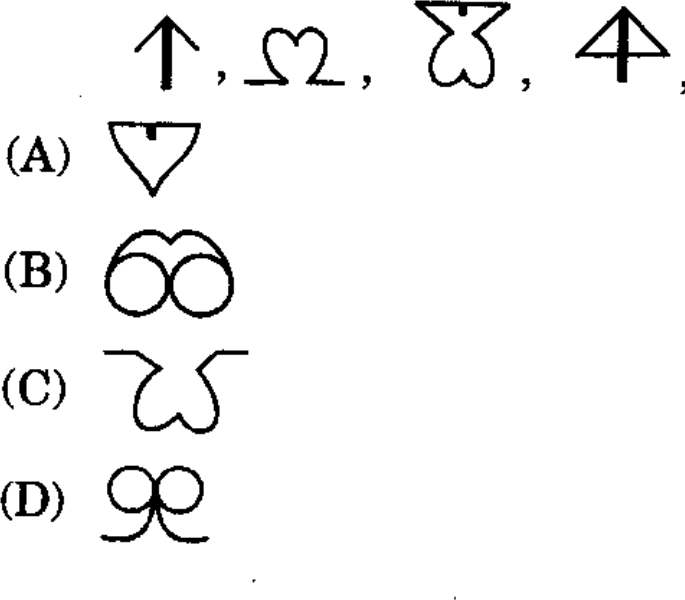
\includegraphics[height=3.6cm]{fig/oct10_q46.png}}
\optsfour{Figure (A)}{Figure (B)}{Figure (C)}{Figure (D)}
\answer{C}{Figure (C)}
\begin{explain}
Each figure is a \textbf{digit joined with its own mirror image}: 1 and its mirror give $\uparrow$, 2 and its mirror give the second shape, then 3 and 4. The next figure must be \textbf{5 joined with its mirror image}, which is figure (C).
\end{explain}
\end{question}

\begin{question}{47}
{If '+' stands for multiplication, '-' stands for division and '*' stands for the power, then the value of [\{(4+3)-2\}*2]-(6*0) is:\par}
\optsfour{30}{25}{35}{20}
\dropped{}
\begin{explain}
Replace the symbols: $[\{(4\times3)\div2\}^2]\div(6^0)=[6^2]\div1=36$.
36 is not among the options, so the agency \textbf{dropped} the question.
\end{explain}
\end{question}

\begin{question}{48}
{Given the correspondence 0 -> -4, 1 -> -3, 2 -> 4, 3 -> 23. Then 3/4 -> ?\par}
\optsfour{520/81}{-341/37}{421/88}{-229/64}
\answer{D}{-229/64}
\begin{explain}
The rule is $x\mapsto x^3-4$: $0-4=-4$, $1-4=-3$, $8-4=4$, $27-4=23$.
\[\left(\tfrac34\right)^3-4=\frac{27}{64}-4=\frac{27-256}{64}=-\frac{229}{64}\]
\end{explain}
\end{question}

\begin{question}{49}
{A person X is taller than Y but shorter than Z. The person V is taller than X but shorter than Z, and W is taller than Y but shorter than X. Then the tallest person will be :\par}
\optsfour{Y}{Z}{V}{X}
\answer{B}{Z}
\begin{explain}
Z $>$ V $>$ X $>$ W $>$ Y, so \textbf{Z} is the tallest.
\end{explain}
\end{question}

\begin{question}{50}
{Make the sequence x, ?, p, l, h. Complete by filling correct answer from the given alternatives.\par}
\optsfour{y}{t}{z}{n}
\answer{B}{t}
\begin{explain}
Positions decrease by 4: x(24), \textbf{t(20)}, p(16), l(12), h(8).
\end{explain}
\end{question}

\begin{question}{51}
{A teacher is teaching in a classroom. The Venn diagram related to school, teacher, classroom and blackboard will be:\par}
\optsfour{\tikz[baseline=-0.5ex,scale=0.3]{\draw (0,0) circle(1.3); \draw (-0.6,0) circle(0.35); \draw (0.6,0) circle(0.4); \draw (0.6,0) circle(0.2);}}{\tikz[baseline=-0.5ex,scale=0.3]{\draw (0,0) circle(1.3); \draw (0,0.7) circle(0.3); \draw (-0.6,-0.3) circle(0.3); \draw (0.6,-0.3) circle(0.3);}}{\tikz[baseline=-0.5ex,scale=0.3]{\draw (0,0) circle(1.3); \draw (0,0) circle(0.85); \draw (-0.3,0) circle(0.25); \draw (0.3,0) circle(0.25);}}{None of (A), (B), (C)}
\answer{C}{\tikz[baseline=-0.5ex,scale=0.3]{\draw (0,0) circle(1.3); \draw (0,0) circle(0.85); \draw (-0.3,0) circle(0.25); \draw (0.3,0) circle(0.25);}}
\begin{explain}
The \textbf{school} contains the \textbf{classroom}, and inside the classroom are the \textbf{teacher} and the \textbf{blackboard} (two separate things). So two small separate circles lie inside the classroom circle, which lies inside the school circle, as in diagram (C).
\end{explain}
\end{question}

\begin{question}{52}
{Fill the correct letter from the given alternatives, in place of question-mark:\\[3pt]
\centering\begin{tabular}{ccc}
\begin{tabular}{|c|c|}\hline C & H\\\hline\multicolumn{2}{|c|}{E}\\\hline R & M\\\hline\end{tabular} &
\begin{tabular}{|c|c|}\hline A & G\\\hline\multicolumn{2}{|c|}{F}\\\hline S & M\\\hline\end{tabular} &
\begin{tabular}{|c|c|}\hline H & J\\\hline\multicolumn{2}{|c|}{?}\\\hline N & L\\\hline\end{tabular}\\
\end{tabular}\par}
\optsfour{C}{K}{B}{O}
\answer{C}{B}
\begin{explain}
The centre letter's position is the difference between the two top letters:
H(8) $-$ C(3) $=5=$ E; G(7) $-$ A(1) $=6=$ F; J(10) $-$ H(8) $=2=$ \textbf{B}.
\end{explain}
\end{question}

\begin{question}{53}
{Put the correct letter in the diagram, from the given alternatives, to replace `?':\\[3pt]
\centering
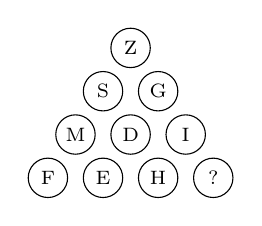
\begin{tikzpicture}[every node/.style={circle,draw,inner sep=1pt,minimum size=5mm,font=\scriptsize}]
\node at (0,0) {Z}; \node at (-0.35,-0.55) {S}; \node at (0.35,-0.55) {G};
\node at (-0.7,-1.1) {M}; \node at (0,-1.1) {D}; \node at (0.7,-1.1) {I};
\node at (-1.05,-1.65) {F}; \node at (-0.35,-1.65) {E}; \node at (0.35,-1.65) {H}; \node at (1.05,-1.65) {?};
\end{tikzpicture}\par}
\optsfour{J}{K}{L}{G}
\answer{D}{G}
\begin{explain}
The positions in every row add up to 26 (Z):
\[\text{S}(19)+\text{G}(7)=26,\quad \text{M}(13)+\text{D}(4)+\text{I}(9)=26\]
\[\text{F}(6)+\text{E}(5)+\text{H}(8)+?=26\Rightarrow ?=7=\mathbf{G}\]
\end{explain}
\end{question}

\begin{question}{54}
{Complete the sequence of squares by choosing the correct figure from the given alternatives:\par}
\qfigure{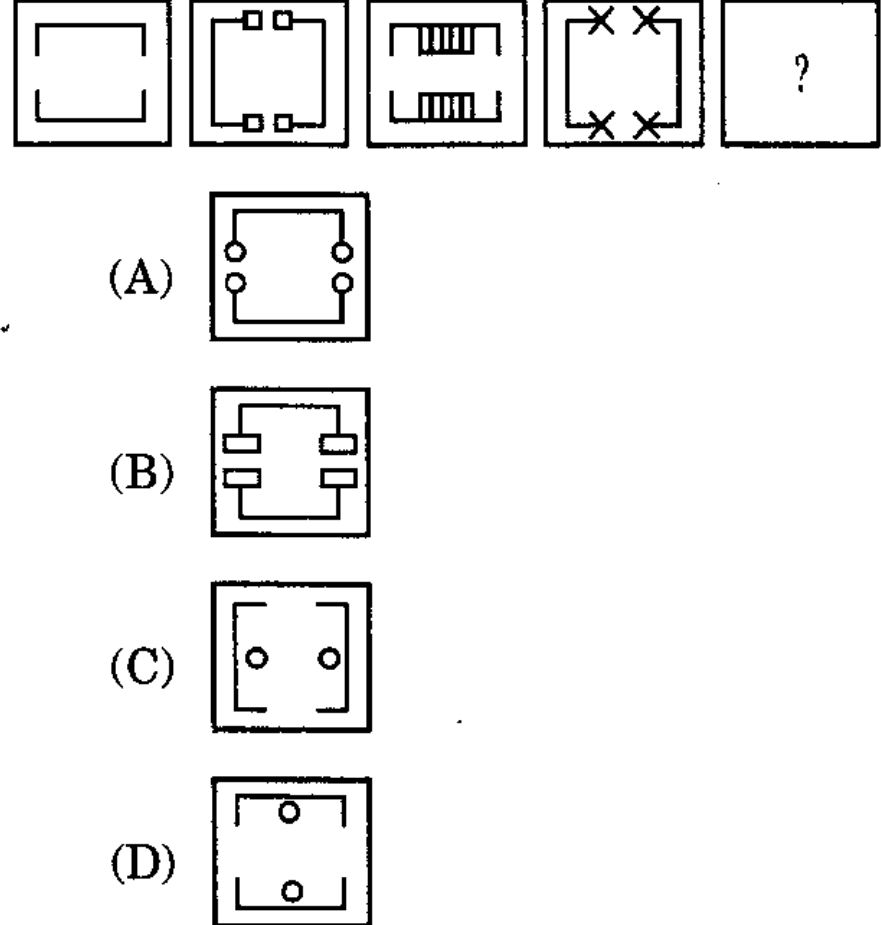
\includegraphics[height=4.6cm]{fig/oct10_q54.png}}
\optsfour{Figure (A)}{Figure (B)}{Figure (C)}{Figure (D)}
\answer{D}{Figure (D)}
\begin{explain}
Two changes alternate. The inner frame alternates between being open on the \emph{sides} and open at the \emph{top and bottom}, and a new decoration appears each time on the \textbf{top and bottom} arms (small squares, hatching, crosses). The fifth figure must again have the frame open like the first and third, with a new element (small circles) on the top and bottom arms, which is figure (D).
\end{explain}
\end{question}

\begin{question}{55}
{Which of the following pollutant gas present in atmosphere is more toxic to human beings ?\par}
\optstwo{Carbon dioxide (CO2)}{Methane (CH4)}{Carbon monoxide (CO)}{Sulphur dioxide (SO2)}
\answer{C}{Carbon monoxide (CO)}
\begin{explain}
\textbf{Carbon monoxide} is the most acutely toxic of these gases. It binds to haemoglobin about 200 times more strongly than oxygen, forming carboxyhaemoglobin and causing suffocation.
\end{explain}
\end{question}

\begin{question}{56}
{Although use of nuclear energy is thought to be pollution free, yet it can pose severe health hazards due to:\par}
\optsone{Nuclear explosion}{Any disaster in nuclear plant}{Unavailability of nuclear waste disposal methods}{Exposure of radiation during normal running of a nuclear plant}
\answer{B}{Any disaster in nuclear plant}
\begin{explain}
Per the key, the chief hazard is \textbf{a disaster in a nuclear plant} (accidents such as Chernobyl 1986 and Fukushima 2011), which releases radioactivity over wide areas.
\end{explain}
\end{question}

\begin{question}{57}
{Green-house effect is increasing due to:\par}
\optsone{Change in atmospheric pressure}{Change in number of green-house gases}{Change in concentration of green-house gases}{Melting of glaciers and dry atmospheric conditions}
\answer{C}{Change in concentration of green-house gases}
\begin{explain}
The greenhouse effect is increasing because the \textbf{concentration} of greenhouse gases (CO$_2$, CH$_4$, N$_2$O) in the atmosphere is rising.
\end{explain}
\end{question}

\begin{question}{58}
{Arrange the following gases in decreasing order of their concentration in atmosphere:\newline (1) Oxygen\newline (2) Nitrogen\newline (3) Carbon dioxide\newline (4) Argon\par}
\optstwo{(2)-(1)-(4)-(3)}{(1)-(2)-(4)-(3)}{(2)-(1)-(3)-(4)}{(2)-(3)-(4)-(1)}
\answer{A}{(2)-(1)-(4)-(3)}
\begin{explain}
Composition of dry air: \textbf{Nitrogen (78\%) $>$ Oxygen (21\%) $>$ Argon (0.93\%) $>$ CO$_2$ ($\approx$0.04\%)}, i.e.\ (2)--(1)--(4)--(3).
\end{explain}
\end{question}

\begin{question}{59}
{Reduction in global warming is possible with:\par}
\optstwo{increased plantation}{conservation of wildlife}{reduction in use of fossil fuel}{(A) and (C)}
\answer{D}{(A) and (C)}
\begin{explain}
Global warming can be reduced by \textbf{increased plantation} (carbon sinks) \textbf{and reduced use of fossil fuels} (fewer emissions), i.e.\ (A) and (C).
\end{explain}
\end{question}

\begin{question}{60}
{Which is the second most important green-house gas besides CO2 responsible for global warming?\par}
\optstwo{Methane}{Chlorofluoro carbon (CFC)}{Nitrous oxide}{Ozone}
\answer{B}{Chlorofluoro carbon (CFC)}
\begin{explain}
Per the key, after CO$_2$ the important greenhouse gas named is \textbf{chlorofluorocarbons (CFCs)}, which have a global-warming potential thousands of times that of CO$_2$.
\tip{By total contribution to warming, methane is usually ranked second after CO$_2$; CFCs are notable for their very high GWP per molecule.}
\end{explain}
\end{question}

\paperchapter{December 2008}{7 December 2008}{C}{50}{GSET 2008}
\keytable{\kcell{1}{C} & \kcell{2}{D} & \kcell{3}{B} & \kcell{4}{D} & \kcell{5}{C} & \kcell{6}{B} & \kcell{7}{C} & \kcell{8}{A} & \kcell{9}{B} & \kcell{10}{A} \\
\kcell{11}{C} & \kcell{12}{C} & \kcell{13}{C} & \kcell{14}{C} & \kcell{15}{B} & \kcell{16}{B} & \kcell{17}{D} & \kcell{18}{A} & \kcell{19}{A} & \kcell{20}{D} \\
\kcell{21}{B} & \kcell{22}{D} & \kcell{23}{A} & \kcell{24}{C} & \kcell{25}{C} & \kcell{26}{C} & \kcell{27}{B} & \kcell{28}{D} & \kcell{29}{C} & \kcell{30}{C} \\
\kcell{31}{A} & \kcell{32}{C} & \kcell{33}{D} & \kcell{34}{D} & \kcell{35}{B} & \kcell{36}{B} & \kcell{37}{A} & \kcell{38}{C} & \kcell{39}{B} & \kcell{40}{C} \\
\kcell{41}{D} & \kcell{42}{A} & \kcell{43}{C} & \kcell{44}{C} & \kcell{45}{D} & \kcell{46}{C} & \kcell{47}{B} & \kcell{48}{C} & \kcell{49}{C} & \kcell{50}{B}}
\begin{question}{1}
{If TEAM is coded as VGCO, then LIFE will be coded as:\par}
\optsfour{NJGE}{NKHF}{NKHG}{NLIH}
\answer{C}{NKHG}
\begin{explain}
Each letter moves \textbf{two places forward}: T$\rightarrow$V, E$\rightarrow$G, A$\rightarrow$C, M$\rightarrow$O.
LIFE $\rightarrow$ L$+2=$N, I$+2=$K, F$+2=$H, E$+2=$G, giving \textbf{NKHG}.
\end{explain}
\end{question}

\begin{question}{2}
{Which of the alternatives will fit in ?\par}
\qfigure{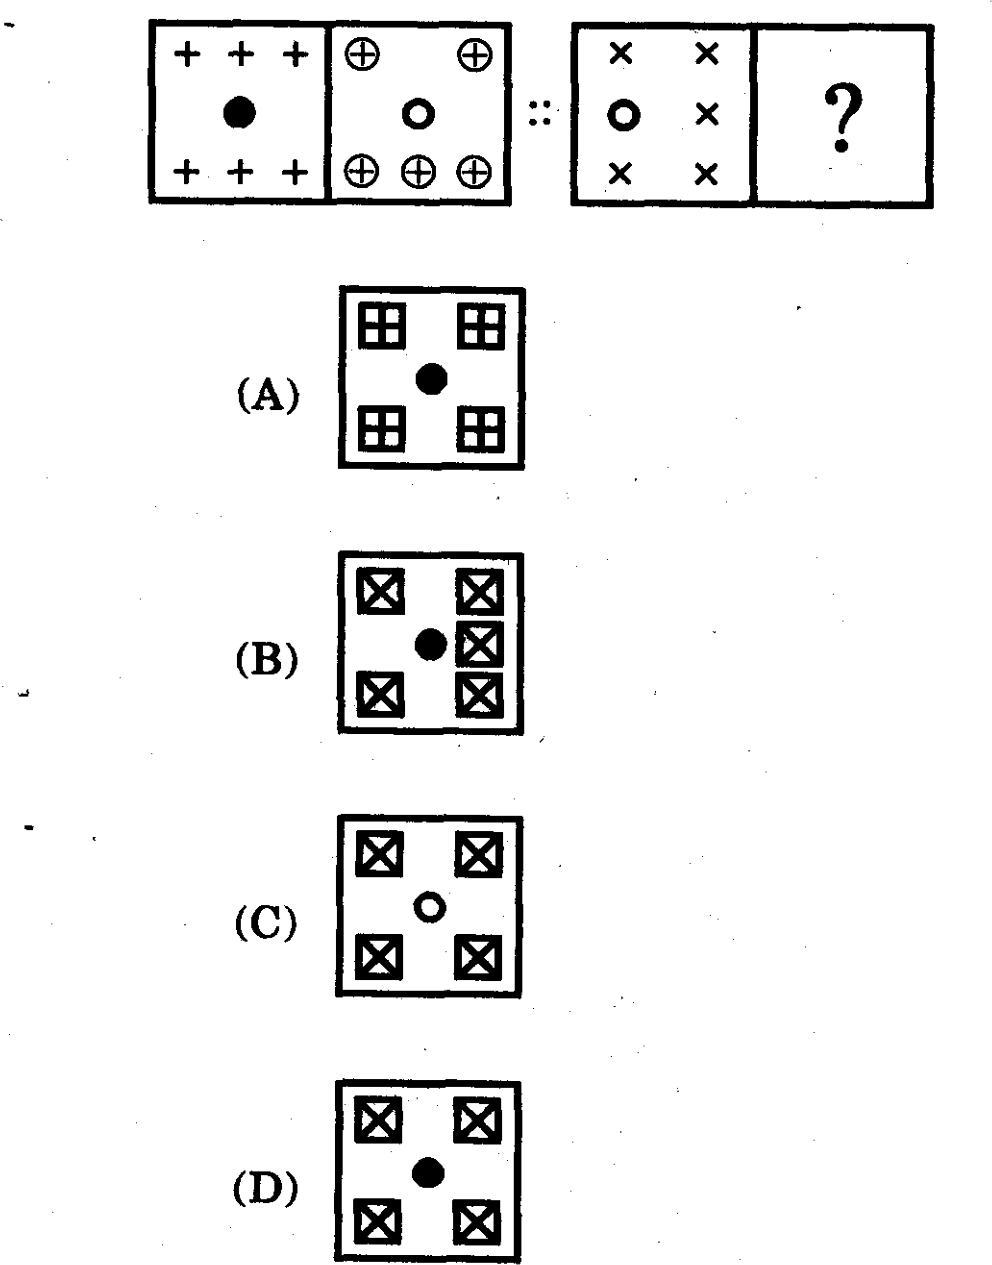
\includegraphics[height=6.2cm]{fig/dec08_q2.png}}
\optsfour{Figure (A)}{Figure (B)}{Figure (C)}{Figure (D)}
\answer{D}{Figure (D)}
\begin{explain}
From the first figure to the second, three things happen. Each symbol is \textbf{enclosed} ($+\rightarrow\oplus$), the number of symbols \textbf{falls by one} ($6\rightarrow5$), and the central dot \textbf{changes shade} (filled $\rightarrow$ hollow).
Apply the same to the third figure: $\times\rightarrow\boxtimes$, $5\rightarrow4$ symbols, and the hollow dot becomes \textbf{filled}. Figure \textbf{(D)} fits.
\why{(A) uses boxed plus signs; (B) has five symbols; (C) keeps the dot hollow.}
\end{explain}
\end{question}

\begin{question}{3}
{How many 7's are there in the following number series which are not followed by 3 but are preceded by 8? 898762263269732872778737794\par}
\optsfour{10}{2}{3}{0}
\answer{B}{2}
\begin{explain}
Look for the pattern ``8 7 x'' where x $\neq 3$:
\begin{center}\ttfamily 8 9 8 \textbf{7} 6 2 2 6 3 2 6 9 7 3 2 8 \textbf{7} 2 7 7 8 7 3 7 7 9 4\end{center}
``8 7 6'' (position 3--5) and ``8 7 2'' qualify, while ``8 7 3'' is excluded. Count $=\mathbf{2}$.
\end{explain}
\end{question}

\begin{question}{4}
{Nitin is counting the numbers in descending order from 32. Shashank is counting the numbers in ascending order from 1 and he pronounces only the odd numbers. If they are counting with the same speed which same number will they pronounce together?\par}
\optstwo{21}{22}{19}{None of the above}
\answer{D}{None of the above}
\begin{explain}
Nitin says 32, 31, 30, \ldots; Shashank says 1, 3, 5, \ldots. At the $n$-th count Nitin says $33-n$ and Shashank says $2n-1$.
$33-n=2n-1\Rightarrow n=34/3$, which is not a whole number, so they \textbf{never say the same number together}: none of the above.
\end{explain}
\end{question}

\begin{question}{5}
{In the following, English letters are used for various symbols: 'B' for addition, 'G' for subtraction, 'E' for multiplication, 'C' for division, 'D' for equal, 'A' for > and 'F' for <. Which of the following is correct?\par}
\optstwo{18C3D6B8C4G12}{18A13B16E8G4E12}{18C3G6B8B4D12}{18A3E6B8G4B12}
\answer{C}{18C3G6B8B4D12}
\begin{explain}
Decode (C): $18\div3-6+8+4=12$, i.e.\ $6-6+8+4=12$ \checkmark.
Check the others: (A) $18\div3=6$ but the right side $8\div4-12$ is not 6; (B) $18>13+128-48$ is false; (D) $18>18+8-4+12=34$ is false.
\end{explain}
\end{question}

\begin{question}{6}
{Numbers are placed in the following figure on the basis of some rules. One place is vacant which is indicated as (?). Find the correct alternative for vacant place.\par}
\qfigure{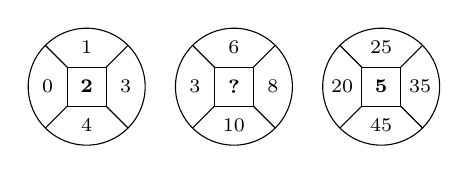
\begin{tikzpicture}[scale=0.55,font=\scriptsize]
\foreach \cx/\t/\l/\r/\b/\c in {0/1/0/3/4/2, 3.4/6/3/8/10/?, 6.8/25/20/35/45/5}{
 \draw (\cx,0) circle(1.35); \draw (\cx-0.45,-0.45) rectangle (\cx+0.45,0.45);
 \draw (\cx-0.45,0.45)--(\cx-0.95,0.95); \draw (\cx+0.45,0.45)--(\cx+0.95,0.95);
 \draw (\cx-0.45,-0.45)--(\cx-0.95,-0.95); \draw (\cx+0.45,-0.45)--(\cx+0.95,-0.95);
 \node at (\cx,0.9){\t}; \node at (\cx-0.9,0){\l}; \node at (\cx+0.9,0){\r}; \node at (\cx,-0.9){\b}; \node at (\cx,0){\textbf{\c}};}
\end{tikzpicture}}
\optsfour{2}{3}{7}{9}
\answer{B}{3}
\begin{explain}
The centre number is the \textbf{cube root of the sum} of the four outer numbers:
\[0+3+1+4=8=2^3,\qquad 20+35+25+45=125=5^3\]
\[3+8+6+10=27=3^3\ \Rightarrow\ ?=\mathbf{3}\]
\end{explain}
\end{question}

\begin{question}{7}
{In a survey of 60 people, it was found that 25 read Newsweek magazine; 26 read Time; 26 read Fortune; 9 read both Newsweek and Fortune; 11 read both Newsweek and Time; 8 read both Time and Fortune and 3 read all magazines. Then number of people who read only Newsweek; Time and Fortune respectively are\par}
\optsfour{7, 10 and 12}{8, 11 and 12}{8, 10 and 12}{8, 10 and 13}
\answer{C}{8, 10 and 12}
\begin{explain}
Let N, T, F be the readers. Only Newsweek $=25-(9+11-3)=25-17=\mathbf{8}$; only Time $=26-(11+8-3)=26-16=\mathbf{10}$; only Fortune $=26-(9+8-3)=26-14=\mathbf{12}$.
\begin{center}
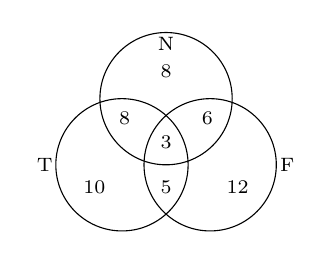
\begin{tikzpicture}[scale=0.7,font=\scriptsize]
\draw (0,0.6) circle(1.2) node[above=14pt]{N}; \draw (-0.8,-0.6) circle(1.2); \draw (0.8,-0.6) circle(1.2);
\node at (0,1.1){8}; \node at (-1.3,-1.0){10}; \node at (1.3,-1.0){12};
\node at (-0.75,0.25){8}; \node at (0.75,0.25){6}; \node at (0,-1.0){5}; \node at (0,-0.2){3};
\node at (-2.2,-0.6){T}; \node at (2.2,-0.6){F};
\end{tikzpicture}
\end{center}
(N$\cap$T only $=11-3=8$, N$\cap$F only $=9-3=6$, T$\cap$F only $=8-3=5$.)
\end{explain}
\end{question}

\begin{question}{8}
{Which of the following best represents the relationship among tennis fans, cricket players and students?\par}
\optsfour{\tikz[baseline=-0.5ex,scale=0.28]{\draw (0,0.45) circle(1); \draw (-0.55,-0.45) circle(1); \draw (0.55,-0.45) circle(1);}}{\tikz[baseline=-0.5ex,scale=0.28]{\draw (0,0) circle(1.3); \draw (0,0.35) circle(0.5); \draw (0,-0.35) circle(0.5);}}{\tikz[baseline=-0.5ex,scale=0.28]{\draw (0,0) circle(0.8); \draw (1.1,0) circle(0.8); \draw (2.2,0) circle(0.8);}}{\tikz[baseline=-0.5ex,scale=0.28]{\draw (0,0) circle(1.2); \draw (0,0) circle(0.9); \draw (0.9,0) circle(0.8);}}
\answer{A}{\tikz[baseline=-0.5ex,scale=0.28]{\draw (0,0.45) circle(1); \draw (-0.55,-0.45) circle(1); \draw (0.55,-0.45) circle(1);}}
\begin{explain}
Tennis fans, cricket players and students can all overlap (a student may play cricket and follow tennis), and none contains another. So we need \textbf{three mutually intersecting circles}, as in diagram (A).
\end{explain}
\end{question}

\begin{question}{9}
{When a parachutist jumps off a plane and the parachute opens, the total force on the man is:\par}
\optstwo{greater than his weight}{less than his weight}{equal to his weight}{zero}
\answer{B}{less than his weight}
\begin{explain}
When the parachute opens, air resistance acts upward. The \textbf{net (total) force} on the man is his weight minus the drag, which is \textbf{less than his weight}. It falls to zero only when he reaches terminal velocity.
\end{explain}
\end{question}

\begin{question}{10}
{Consider the sequence : 0, 1, 1, 2, 3, 5, 8, 13, 21, 34, \ldots{} The next four members of sequence are:\par}
\optstwo{55, 89, 144 and 233}{45, 79, 134 and 223}{65, 99, 154 and 243}{54, 89, 144 and 232}
\answer{A}{55, 89, 144 and 233}
\begin{explain}
This is the \textbf{Fibonacci sequence}: each term is the sum of the previous two. $21+34=55$, $34+55=89$, $55+89=144$, $89+144=233$.
\end{explain}
\end{question}

\begin{question}{11}
{Read the following graph and decide which of the following statement is \emph{false}:\par}
\qfigure{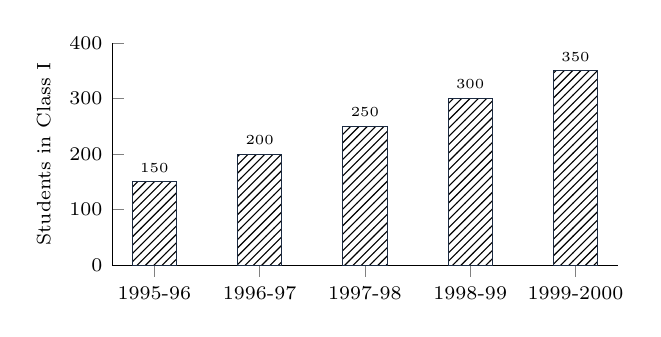
\begin{tikzpicture}
\begin{axis}[ybar,width=8cm,height=4.4cm,bar width=16pt,ymin=0,ymax=400,
  symbolic x coords={1995-96,1996-97,1997-98,1998-99,1999-2000},xtick=data,
  nodes near coords,every node near coord/.append style={font=\tiny},tick label style={font=\scriptsize},
  ylabel={\scriptsize Students in Class I},axis x line*=bottom,axis y line*=left]
\addplot[pattern=north east lines,draw=ink] coordinates {(1995-96,150) (1996-97,200) (1997-98,250) (1998-99,300) (1999-2000,350)};
\end{axis}
\end{tikzpicture}}
\optsone{Number of students in each academic year is divisible by 25}{Number of students in 1999-2000 is more than twice the number in 1995-96}{Number of students in 1995-96: Number of students in 1996-97 is equal to Number of students in 1996-97: No. of students in 1997-98}{The total growth in number of students is not less than 200}
\answer{C}{Number of students in 1995-96: Number of students in 1996-97 is equal to Number of students in 1996-97: No. of students in 1997-98}
\begin{explain}
Values: 150, 200, 250, 300, 350.
(A) all are divisible by 25, true. (B) $350>2\times150=300$, true. (D) total growth $=350-150=200$, which is not less than 200, true.
(C) $150:200=0.75$ but $200:250=0.8$, so the ratios are \textbf{not equal}. Statement (C) is \textbf{false}.
\end{explain}
\end{question}

\begin{question}{12}
{Following the constant growth described in the previous diagram, which year first time there will be more than 1111 students in Class I ?\par}
\optsfour{2010}{2013}{2016}{2020}
\answer{C}{2016}
\begin{explain}
Growth is constant at $+50$ students per year: $350+50n>1111\Rightarrow n>15.22\Rightarrow n=16$.
Sixteen years after 1999--2000 is 2015--16, i.e.\ \textbf{2016}.
\end{explain}
\end{question}

\begin{question}{13}
{A tyre manufacturing company kept a record of the distance covered before a tyre to be replaced. The following table shows the results of 1000 cases:
\begin{center}\small
\begin{tabular}{lc}\toprule Distance (km) & Tyres replaced\\\midrule Less than 400 & 210\\ 400--900 & 325\\ 900--1400 & 385\\ More than 1400 & 80\\\bottomrule\end{tabular}
\end{center}
If you buy a tyre of this company, what is the probability that it will need to be replaced before it has covered 400 km?\par}
\optsfour{0.4}{0.3}{0.21}{0.14}
\answer{C}{0.21}
\begin{explain}
Empirical probability $=\dfrac{210}{1000}=\mathbf{0.21}$.
\end{explain}
\end{question}

\begin{question}{14}
{As a researcher you find that, the correlation between intensity of punishment and students' achievement is -.86. This means that:\par}
\optsone{higher the intensity of punishment greater would be the achievement}{intensity of punishment has no relation with achievement}{increase in the intensity of punishment will decrease achievement of students}{increase in the intensity of punishment may or may not decrease the achievement of students}
\answer{C}{increase in the intensity of punishment will decrease achievement of students}
\begin{explain}
A correlation of $-0.86$ is a \textbf{high negative} correlation: as the intensity of punishment increases, achievement tends to \textbf{decrease}.
\tip{Correlation shows association, not proof of causation, but in exam language this is read as ``more punishment, lower achievement''.}
\end{explain}
\end{question}

\begin{question}{15}
{In an experimental study you want to study the effectiveness of method of teaching A and B. Each group has 50 randomly selected students. Appropriate technique of data analysis will be :\par}
\optstwo{chi-square test}{t-test}{F-test}{multiple regression}
\answer{B}{t-test}
\begin{explain}
Comparing the means of \textbf{two independent groups} (method A vs method B), each of 50 students, calls for the \textbf{t-test}.
\why{Chi-square is for frequencies; the F-test (ANOVA) is for three or more groups; regression is for prediction.}
\end{explain}
\end{question}

\begin{question}{16}
{Which of the following is used to connect two LAN using same LAN protocols over a wide area ?\par}
\optstwo{Router}{Bridges}{Gateways}{None of the above}
\answer{B}{Bridges}
\begin{explain}
Per the key, \textbf{bridges} connect two LANs that use the same protocol. (Bridges work at the data-link layer; routers connect different networks.)
\end{explain}
\end{question}

\begin{question}{17}
{Which of the following are switching techniques ?\par}
\optstwo{Circuit switching}{Message switching}{Packet switching}{Each of the above three techniques}
\answer{D}{Each of the above three techniques}
\begin{explain}
Circuit switching (telephone), message switching (store-and-forward) and packet switching (Internet) are all switching techniques: \textbf{each of the three}.
\end{explain}
\end{question}

\begin{question}{18}
{Protocol is used to communicate between:\par}
\optstwo{similar module}{dissimilar module}{both (A) and (B)}{none of the above}
\answer{A}{similar module}
\begin{explain}
A \textbf{protocol} is a set of rules for communication between \textbf{similar (peer) modules}, i.e.\ the same layer in two systems.
\end{explain}
\end{question}

\begin{question}{19}
{Data transfer rate for LAN is normally:\par}
\optstwo{1-100 Mbps}{1-2 Mbps}{1-10 Mbps}{None of the above}
\answer{A}{1-100 Mbps}
\begin{explain}
Typical LAN data rates are \textbf{1--100 Mbps} (Ethernet 10/100 Mbps in that period).
\end{explain}
\end{question}

\begin{question}{20}
{Which of the following are WAN devices ?\par}
\optstwo{Bridges}{Routers}{Gateways}{Each of the above three devices}
\answer{D}{Each of the above three devices}
\begin{explain}
Bridges, routers and gateways are all used in wide-area networking: \textbf{each of the three devices}.
\end{explain}
\end{question}

\begin{question}{21}
{Mushrooms form a promising source of:\par}
\optstwo{carbohydrate}{protein}{minerals}{carbohydrate plus lipid}
\answer{B}{protein}
\begin{explain}
Mushrooms are valued as a promising source of \textbf{protein} (with vitamins and minerals), especially for vegetarians.
\end{explain}
\end{question}

\begin{question}{22}
{Nuclear energy can be obtained from:\par}
\optsone{fission of radioactive material}{synthetic reactions of radioactive material}{fusion of radioactive material}{both fission and fusion of radioactive material}
\answer{D}{both fission and fusion of radioactive material}
\begin{explain}
Nuclear energy comes from both \textbf{fission} (splitting heavy nuclei such as U-235) and \textbf{fusion} (joining light nuclei, as in the Sun).
\end{explain}
\end{question}

\begin{question}{23}
{Petroplants are the sources of:\par}
\optstwo{liquid hydrocarbon}{liquid nitrogen}{liquid fuels}{alcohols}
\answer{A}{liquid hydrocarbon}
\begin{explain}
\textbf{Petroplants} (e.g.\ \emph{Euphorbia}, \emph{Jatropha}) yield latex rich in \textbf{liquid hydrocarbons} that can substitute for petroleum.
\end{explain}
\end{question}

\begin{question}{24}
{Occupational diseases result from:\par}
\optstwo{malnutrition}{overworking}{toxic chemical residues}{unadequate basic amenities}
\answer{C}{toxic chemical residues}
\begin{explain}
Occupational diseases (silicosis, asbestosis, lead poisoning) result from exposure to \textbf{toxic chemicals, dusts and residues} at the workplace.
\end{explain}
\end{question}

\begin{question}{25}
{Which one among the following is a non-commercial sources of energy ?\par}
\optstwo{Coal}{Oil}{Agricultural waste}{Electricity}
\answer{C}{Agricultural waste}
\begin{explain}
\textbf{Agricultural waste} (together with firewood and cow dung) is a \textbf{non-commercial} energy source: it is not usually bought and sold. Coal, oil and electricity are commercial.
\end{explain}
\end{question}

\begin{question}{26}
{The research in education has not given due importance to:\par}
\optstwo{adolescent student's problems}{adolescent learning styles}{adult student's learning styles}{children's learning styles}
\answer{C}{adult student's learning styles}
\begin{explain}
Educational research has concentrated on children and adolescents and has given relatively little importance to \textbf{adult students' learning styles} (andragogy).
\end{explain}
\end{question}

\begin{question}{27}
{Linking Career Advancement Scheme with research publications:\par}
\optsone{enhances quality of research due to increase in quantity}{deteriorates quality of research due to increase in quantity}{enhances quality of research as fund of knowledge is greater}{does not influence quality of research}
\answer{B}{deteriorates quality of research due to increase in quantity}
\begin{explain}
Per the key, linking career advancement to the number of publications \textbf{deteriorates quality}: it encourages quantity over quality (``publish or perish'', predatory journals).
\end{explain}
\end{question}

\begin{question}{28}
{Which of the following IGNOU does not prescribe ?\par}
\optsone{Flexibility to eligibility for enrolment}{Relaxation of age of entry}{Flexibility to methods of evaluation}{Strict combination of courses of study}
\answer{D}{Strict combination of courses of study}
\begin{explain}
IGNOU offers flexibility in eligibility, age of entry, pace and evaluation. It does \emph{not} prescribe a \textbf{strict combination of courses}; learners may choose.
\end{explain}
\end{question}

\begin{question}{29}
{Spiritual value never cherishes:\par}
\optstwo{non-violence}{respect for all religions}{untouchability}{truth}
\answer{C}{untouchability}
\begin{explain}
Spiritual values include non-violence, truth and respect for all religions. \textbf{Untouchability} contradicts them (it is also abolished by Article 17).
\end{explain}
\end{question}

\begin{question}{30}
{The POA of NPE, 1992 does not envisage:\par}
\optsone{making education a mass movement}{special emphasis on education of girls}{making English as compulsory language for all}{establishment of pace-setting institutions}
\answer{C}{making English as compulsory language for all}
\begin{explain}
The Programme of Action (1992) of NPE 1986 aimed at a mass movement for education, girls' education and pace-setting institutions (Navodaya Vidyalayas). It did not make \textbf{English compulsory for all}.
\end{explain}
\end{question}

\begin{question}{31}
{Which is not the aim of education ?\par}
\optsone{Completing the syllabus in stipulated time}{Inculcating cognitive competence through subject teaching}{Developing citizenship in the students}{Equipping students with life skills}
\answer{A}{Completing the syllabus in stipulated time}
\begin{explain}
\textbf{Completing the syllabus in stipulated time} is an administrative target, not an aim of education.
\end{explain}
\end{question}

\begin{question}{32}
{What will you do to update your competence of teaching?\par}
\optsone{Read books on methods of teaching}{Visit different websites on teaching techniques}{Experimenting with a variety of classroom activities}{Seek guidance from senior teachers}
\answer{C}{Experimenting with a variety of classroom activities}
\begin{explain}
The best way to update teaching competence is to \textbf{experiment with a variety of classroom activities}, i.e.\ reflective practice and learning by doing.
\end{explain}
\end{question}

\begin{question}{33}
{If a learner can use an abstraction-a rule, a principle or an idea in particular and concrete situations, then he has reached the level of educational objective:\par}
\optsfour{comprehension}{analysis}{synthesis}{application}
\answer{D}{application}
\begin{explain}
Using an abstraction (rule, principle) in particular, concrete situations is \textbf{application} in Bloom's taxonomy.
\end{explain}
\end{question}

\begin{question}{34}
{How is the working model valued ?\par}
\optsone{By recognition of external features}{By seeing the internal structure}{By seeing both external and internal structures}{By following actions and processes as they develop}
\answer{D}{By following actions and processes as they develop}
\begin{explain}
A working model is valued for \textbf{showing actions and processes as they develop}, i.e.\ how the thing actually works.
\end{explain}
\end{question}

\begin{question}{35}
{Adolescents' problems may be handled by those teachers who have skills of:\par}
\optsfour{Managers}{Counsellors}{Psychiatrists}{Therapists}
\answer{B}{Counsellors}
\begin{explain}
Adolescents' problems are best handled by teachers with \textbf{counselling} skills.
\end{explain}
\end{question}

\begin{question}{36}
{In research operational definition of a variable means:\par}
\optsone{considering different definitions and giving one's own as taken in the present study}{stipulating tasks by which variables can be observed and measured}{explaining operationality to make concept clear}{stipulating concept in all its constituents}
\answer{B}{stipulating tasks by which variables can be observed and measured}
\begin{explain}
An \textbf{operational definition} states the operations or tasks by which a variable is \textbf{observed and measured} (e.g.\ ``achievement $=$ score on test X'').
\end{explain}
\end{question}

\begin{question}{37}
{In an experimental research, it is essential that researcher :\par}
\optsone{directly controls and manipulates variables}{must take things as they are in an experiment}{must manipulate the variable but need not control}{must control the variable but need not manipulate}
\answer{A}{directly controls and manipulates variables}
\begin{explain}
In experimental research the researcher \textbf{directly manipulates} the independent variable and \textbf{controls} extraneous variables.
\end{explain}
\end{question}

\begin{question}{38}
{The research aims at understanding reality, discovering new knowledge and inventions for development in the society and research ethics certainly can restrain researchers. Considering all aspects it is amicably decided that researchers :\par}
\optsone{will have complete freedom for research}{will not conduct studies involving risks to human beings}{will follow some code of research ethics}{will decide research ethics themselves}
\answer{C}{will follow some code of research ethics}
\begin{explain}
Research must balance freedom and responsibility, so researchers \textbf{follow a code of research ethics} (informed consent, confidentiality, avoidance of harm).
\end{explain}
\end{question}

\begin{question}{39}
{The law of probability is applied in:\par}
\optstwo{purposive sampling}{random sampling}{quota sampling}{convenient sampling}
\answer{B}{random sampling}
\begin{explain}
The law of probability applies to \textbf{random sampling}, where each unit has a known, equal chance of selection.
\end{explain}
\end{question}

\begin{question}{40}
{If a researcher wants to study the performance of university teachers by students which tool will be most appropriate ?\par}
\optstwo{Questionnaire}{Interview}{Rating scale}{Observation schedule}
\answer{C}{Rating scale}
\begin{explain}
To obtain students' evaluation of teacher performance on various dimensions, a \textbf{rating scale} is the most appropriate tool.
\end{explain}
\end{question}

\begin{context}
\textbf{Direction (Q.~Nos.~41 to 45):} Read the following text and answer the questions that follow.\par\smallskip
Human decision-making is being influenced profoundly by modern mathematics, and several particular mathematical subjects have been created primarily to assist in arriving at good decisions. Many aspects involved in arriving at a decision are, of course, nonquantitative in nature. These may relate to history, past experience, instinct, judgement, morality, and so forth. As a consequence, one often refers to decision-making as an art. On the other hand, many ingredients in contemporary decision-making are mathematical in nature, and one can also view this activity as a science.

A decision maker will begin by listing the options over which he or she has some control and the likely outcomes resulting from these choices. The person may attempt to identify all relevant variables and the relationships among them and may associate quantitative measures when possible. Moreover, the decision maker must clarify his or her own values, identify desired goals, and spell out explicitly any limiting resources or social constraints. One then seeks the best possible result obtainable. The situation is typically confounded by a variety of different uncertainties involving data and forecasting that typically cannot be completely resolved in advance. The effect that other decision makers may have on the outcome, and the best responses to their moves, should be predetermined. Various ethical concerns such as fairness may well need consideration, and ways to ascertain group opinions may be necessary. Finally, decision makers must study the social and political context in which the decision will be implemented.
\end{context}
\begin{question}{41}
{What is the central idea of this paragraph ?\par}
\optsone{Decision-making is a mathematical activity}{Decision-making is a complex intellectual activity}{Decision-making is almost impossible}{Decision-making is also emotional and social in nature}
\answer{D}{Decision-making is also emotional and social in nature}
\begin{explain}
The passage stresses that besides mathematics, decision-making involves non-quantitative aspects (history, instinct, judgement, morality), group opinion and the social--political context. Per the key, the central idea is that it is \textbf{also emotional and social in nature}.
\end{explain}
\end{question}

\begin{question}{42}
{What is the major source of puzzlement in decision-making ?\par}
\optsone{An exact prediction of the results of the decision}{Socio-political context}{Ignorance of Mathematics}{Lack of adequate practice}
\answer{A}{An exact prediction of the results of the decision}
\begin{explain}
The situation ``is typically confounded by a variety of different uncertainties involving data and forecasting that typically cannot be completely resolved in advance'', i.e.\ the difficulty of \textbf{exactly predicting the results}.
\end{explain}
\end{question}

\begin{question}{43}
{Which step is not inevitable in the process of decision-making ?\par}
\optsone{Recognizing the factors affecting the process}{Thinking of the end product one would wish to achieve}{Using quantitative measures}{Forecasting outcomes in advance}
\answer{C}{Using quantitative measures}
\begin{explain}
The decision maker ``may associate quantitative measures \textbf{when possible}'', so using quantitative measures is \textbf{not inevitable}. The other steps are described as necessary.
\end{explain}
\end{question}

\begin{question}{44}
{Decision-making is an art, because:\par}
\optsone{it involves a lot of variables}{it depends upon a person's multiple abilities}{it entails some personal perspectives}{it does not ensure the best outcome}
\answer{C}{it entails some personal perspectives}
\begin{explain}
Decision-making is called an art because many aspects are non-quantitative: history, experience, instinct, judgement, morality, i.e.\ it \textbf{entails personal perspectives}.
\end{explain}
\end{question}

\begin{question}{45}
{"Various ethical concerns such as fairness may well need consideration" means:\par}
\optsone{a decision is value-free}{it is fair to think about needs of people affected by the decision}{your decision must do justice to all}{morality is a criterion of a good decision}
\answer{D}{morality is a criterion of a good decision}
\begin{explain}
Considering ethical concerns such as fairness implies that \textbf{morality is a criterion of a good decision}.
\end{explain}
\end{question}

\begin{question}{46}
{A student is speaking fast with irregular rhythm and long breaks in between. This indicates :\par}
\optstwo{excitement}{sense of purpose}{nervousness}{frustration}
\answer{C}{nervousness}
\begin{explain}
Fast speech with irregular rhythm and long pauses is a paralinguistic sign of \textbf{nervousness} (anxiety).
\end{explain}
\end{question}

\begin{question}{47}
{What does 'You' attitude imply in spoken or written communication ?\par}
\optsone{Think and express from the sender's point of view}{Think and express from the receiver's point of view}{Give maximum opportunity to the listener for expression}{Never forget who you are}
\answer{B}{Think and express from the receiver's point of view}
\begin{explain}
The \textbf{``You'' attitude} means writing or speaking from the \textbf{receiver's point of view}: their needs, interests and benefits.
\end{explain}
\end{question}

\begin{question}{48}
{A speech that is outlined, practised and delivered in a conversation style is:\par}
\optstwo{hat speech}{indirect speech}{extemporaneous}{manuscripted}
\answer{C}{extemporaneous}
\begin{explain}
A speech that is outlined, practised and delivered conversationally from notes (not memorised or read out) is \textbf{extemporaneous}.
\why{A manuscript speech is read verbatim; an impromptu speech is unprepared.}
\end{explain}
\end{question}

\begin{question}{49}
{To communicate effectively with college level students, the teacher requires:\par}
\optsone{to keep appropriate distance with the students}{to have mastery over the subject}{to know his students well}{to look directly into the eyes of the students}
\answer{C}{to know his students well}
\begin{explain}
To communicate effectively with college students the teacher must \textbf{know the students well}: their background, level, interests and needs.
\end{explain}
\end{question}

\begin{question}{50}
{Which factor leads to the most successful communication ?\par}
\optsone{Speaker's knowledge about the process of communication}{Empathy with the receiver}{Use of multiple channels}{Admiration from the receiver}
\answer{B}{Empathy with the receiver}
\begin{explain}
\textbf{Empathy with the receiver}, i.e.\ understanding the receiver's feelings and viewpoint, leads to the most successful communication.
\end{explain}
\end{question}

\paperchapter{July 2006}{July 2006}{A}{50}{GSET 2006}
\keytable{\kcell{1}{B} & \kcell{2}{C} & \kcell{3}{A} & \kcell{4}{A} & \kcell{5}{C} & \kcell{6}{B} & \kcell{7}{A} & \kcell{8}{B} & \kcell{9}{A} & \kcell{10}{D} \\
\kcell{11}{D} & \kcell{12}{B} & \kcell{13}{C} & \kcell{14}{A} & \kcell{15}{A} & \kcell{16}{D} & \kcell{17}{A} & \kcell{18}{C} & \kcell{19}{D} & \kcell{20}{B} \\
\kcell{21}{A} & \kcell{22}{C} & \kcell{23}{C} & \kcell{24}{C} & \kcell{25}{D} & \kcell{26}{D} & \kcell{27}{D} & \kcell{28}{B} & \kcell{29}{A} & \kcell{30}{D} \\
\kcell{31}{C} & \kcell{32}{B} & \kcell{33}{D} & \kcell{34}{A} & \kcell{35}{B} & \kcell{36}{C} & \kcell{37}{A} & \kcell{38}{B} & \kcell{39}{A} & \kcell{40}{A} \\
\kcell{41}{C} & \kcell{42}{B} & \kcell{43}{A} & \kcell{44}{C} & \kcell{45}{D} & \kcell{46}{D} & \kcell{47}{B} & \kcell{48}{D} & \kcell{49}{A} & \kcell{50}{B}}
\begin{question}{1}
{Which one of the following is the most important characteristics of a good teacher?\par}
\optstwo{To control the class effectively.}{To motivate the students for learning}{To have command over the subject}{To use different teaching methods.}
\answer{B}{To motivate the students for learning}
\begin{explain}
The most important quality of a good teacher is the ability to \textbf{motivate students to learn}. Motivation drives attention, effort and lifelong learning; mastery of subject and methods serve this end.
\end{explain}
\end{question}

\begin{question}{2}
{During the teaching-learning process a teacher should\par}
\optsone{provide relevant information}{maintain a lively classroom environment}{allow students to raise questions}{give relevant illustrations.}
\answer{C}{allow students to raise questions}
\begin{explain}
During teaching, a teacher should \textbf{allow students to raise questions}. Questions show engagement, clarify doubts and make learning two-way.
\end{explain}
\end{question}

\begin{question}{3}
{The ultimate goal of education is to\par}
\optsone{develop problem-solving skills among students}{make students economically productive}{cultivate the habit of maintaining good relationships}{prepare knowledgeable individuals.}
\answer{A}{develop problem-solving skills among students}
\begin{explain}
Per the key, the ultimate goal of education is to \textbf{develop problem-solving skills} so that learners can face real-life situations independently.
\end{explain}
\end{question}

\begin{question}{4}
{The main function of teachers in higher education is\par}
\optstwo{teaching, research and extension.}{being a friend, philosopher and guide.}{to solve problems of students.}{to generate knowledge.}
\answer{A}{teaching, research and extension.}
\begin{explain}
The main functions of teachers in higher education are \textbf{teaching, research and extension} (service to the community), the three pillars of universities.
\end{explain}
\end{question}

\begin{question}{5}
{If a student asks you a question in the class the answer of which you do not know, then what will you do?\par}
\optsone{Get angry with the student.}{Do not allow anyone to ask questions.}{Accept your lack of knowledge and tell that you will come prepared with the same next time.}{Will feel guilty.}
\answer{C}{Accept your lack of knowledge and tell that you will come prepared with the same next time.}
\begin{explain}
An honest teacher \textbf{accepts the lack of knowledge} and promises to come prepared next time, modelling integrity and a learning attitude.
\end{explain}
\end{question}

\begin{question}{6}
{Which one of the following is not the aim of scientific research?\par}
\optstwo{Theory building.}{Logical reasoning.}{Problem solving.}{Creating new knowledge.}
\answer{B}{Logical reasoning.}
\begin{explain}
Scientific research aims at theory building, problem solving and creating new knowledge. \textbf{Logical reasoning} is a \emph{means} (a tool) of research, not its aim.
\end{explain}
\end{question}

\begin{question}{7}
{An investigator studied some selected subjects for certain years continuously. The type of research is:\par}
\optstwo{Longitudinal study.}{Cross-sectional study.}{Experimental study.}{Correlational study.}
\answer{A}{Longitudinal study.}
\begin{explain}
Studying the same subjects repeatedly over several years is a \textbf{longitudinal study}. A cross-sectional study observes different groups at one point in time.
\end{explain}
\end{question}

\begin{question}{8}
{Which one is the most important factor for selection of a research problem?\par}
\optstwo{Researcher's interest.}{Researchability of the problem.}{Administrative suitability.}{Uniqueness of the problem.}
\answer{B}{Researchability of the problem.}
\begin{explain}
The most important factor is \textbf{researchability}: whether the problem can be studied empirically with available data, tools, time and resources.
\end{explain}
\end{question}

\begin{question}{9}
{Inductive reasoning implies\par}
\optstwo{particular to general.}{general to particular.}{symbolic logic.}{none of the above.}
\answer{A}{particular to general.}
\begin{explain}
\textbf{Inductive} reasoning moves from \textbf{particular to general} (specific observations $\rightarrow$ general conclusion). Deduction moves from general to particular.
\end{explain}
\end{question}

\begin{question}{10}
{Which one of the following is not the example of qualitative research?\par}
\optstwo{Case study.}{Ethnography.}{Content analysis.}{Pretest-Posttest experiment.}
\answer{D}{Pretest-Posttest experiment.}
\begin{explain}
Case study, ethnography and content analysis are qualitative. A \textbf{pretest--posttest experiment} is a quantitative experimental design.
\end{explain}
\end{question}

\begin{context}
\textbf{Direction (Q.~No.~11 to 15):} Read the following text and answer questions 11 to 15.\par\smallskip
Sixty per cent of rural India lives in utter poverty with no electricity. Rural India uses 180 million tones of fuel every year for cooking, creating indoor pollution and health hazards. The WHO estimates that 1.5 million deaths per year are caused by pollution from chulha smoke. Making available locally grown clean and renewable cooking and lighting fuel can improve the quality of rural life. Liquid fuels are far superior to solid fuels for cooking because of their clean burning and higher energy. Ethanol is one of the best as it is an excellent substitute for kerosene and burns better with no unpleasant smell. Its burning power is almost as clean as that of LPG.

Ethanol can be produced from any sugary material and is presently produced world over from sugarcane and corn. However, as the ethanol economy grows, there is need to produce it from a crop which uses much less water than sugarcane and also produces food. Sorghum (Jowar) is one such crop whose stem is sweet like sugarcane. Its earhead produces grains which can be used for making bread. Its sweet stem has nearly the same amount of sugar and hence the juice can be fermented and used for ethanol production. The left-over stem after juice extraction, together with leaves is excellent fodder for animals. So from the same price of land one can get food, fuel and fodder. Besides, sweet sorghum (Jowar) uses nearly fifty percent less water than sugarcane to produce the same amount of sugar. It is a four month crop so farmers can grow two crops per year from the same piece of land. Also the energy output ratio from sweet sorghum is very positive.
\end{context}
\begin{question}{11}
{The purpose of the paragraph is to bring out:\par}
\optstwo{Problems of rural poor.}{The limitations of sugar cane.}{Benefits of sorghum (Jowar).}{Remedies for pollutant energy.}
\answer{D}{Remedies for pollutant energy.}
\begin{explain}
The paragraph identifies a problem (polluting solid cooking fuels) and proposes a solution: clean, locally grown ethanol from sweet sorghum. Its purpose is to bring out \textbf{remedies for pollutant energy}.
\end{explain}
\end{question}

\begin{question}{12}
{Most suitable heading for the paragraph will be:\par}
\optstwo{Rural poverty.}{Alternate Fuels.}{Solid Fuels Vs. Liquid Fuels.}{Efficient Fuels.}
\answer{B}{Alternate Fuels.}
\begin{explain}
The passage argues for \textbf{alternate fuels} (ethanol from sweet sorghum) in place of polluting solid fuels.
\end{explain}
\end{question}

\begin{question}{13}
{As per the authors, who are the rural poor?\par}
\optsone{Who do not have any electricity.}{Who use solid fuel for cooking.}{Who live with pollution and health hazards.}{Who do not use cooking gas.}
\answer{C}{Who live with pollution and health hazards.}
\begin{explain}
Per the key, the rural poor are those \textbf{who live with pollution and health hazards} (from chulha smoke, with no electricity).
\end{explain}
\end{question}

\begin{question}{14}
{As per the author which can be easy source of energy\par}
\optsone{fuel that can be locally produced.}{fuel that can be produced from crops.}{fuel that can be used as alternate to kerosene.}{fuel that does not give unpleasant smell.}
\answer{A}{fuel that can be locally produced.}
\begin{explain}
``Making available \textbf{locally grown} clean and renewable cooking and lighting fuel can improve the quality of rural life.''
\end{explain}
\end{question}

\begin{question}{15}
{The nature of the paragraph is\par}
\optsfour{analytical.}{critical.}{conceptual.}{comprehensive.}
\answer{A}{analytical.}
\begin{explain}
The paragraph analyses the problem and compares crops and fuels using evidence (water use, energy output ratio), so it is \textbf{analytical}.
\end{explain}
\end{question}

\begin{question}{16}
{Students are inattentive in the classroom. The reason is:\par}
\optstwo{Lack of interest in the subject.}{Outside obstacles.}{Nature of the subject.}{Poor communication.}
\answer{D}{Poor communication.}
\begin{explain}
Inattention in class usually signals \textbf{poor communication} by the teacher: unclear, monotonous or irrelevant presentation.
\end{explain}
\end{question}

\begin{question}{17}
{Communication is a network of\par}
\optstwo{Interactions.}{Messages.}{Receivers and senders.}{Information.}
\answer{A}{Interactions.}
\begin{explain}
Communication is a network of \textbf{interactions} between people: a dynamic two-way process, not just messages or information.
\end{explain}
\end{question}

\begin{question}{18}
{Which one of the following is not a barrier to communication ?\par}
\optstwo{Noise.}{Culture.}{Job satisfaction.}{Attitude.}
\answer{C}{Job satisfaction.}
\begin{explain}
Noise, culture and attitude can be barriers. \textbf{Job satisfaction} is not a barrier to communication.
\end{explain}
\end{question}

\begin{question}{19}
{Which of the following is true with respect to a good communicator?\par}
\optsone{May not always be a good teacher.}{Has humourous expression.}{Has a wise range of reading interest.}{Has mastery over the medium of instruction.}
\answer{D}{Has mastery over the medium of instruction.}
\begin{explain}
A good communicator \textbf{has mastery over the medium of instruction}, i.e.\ command of language and channel.
\end{explain}
\end{question}

\begin{question}{20}
{Which of the following are the important characteristics of an effective teacher ?\newline (i) Knowledge of content.\newline (ii) Effective verbal communication skills.\newline (iii) Impressive personality.\newline (iv) Ability to command respect from students.\par}
\optsfour{(ii) and (iii)}{(i) and (ii)}{(iii) and (iv)}{(i) and (iv).}
\answer{B}{(i) and (ii)}
\begin{explain}
The most important characteristics of an effective teacher are \textbf{knowledge of content (i)} and \textbf{effective verbal communication (ii)}.
\end{explain}
\end{question}

\begin{question}{21}
{Find the odd number out: 8, 9, 64, 125, 216, 49\par}
\optsfour{125}{216}{64}{49}
\answer{A}{125}
\begin{explain}
The numbers alternate cube and square: $2^3=8$, $3^2=9$, $4^3=64$, $5^2=25$, $6^3=216$, $7^2=49$. \textbf{125} breaks the pattern (it should be 25).
\end{explain}
\end{question}

\begin{question}{22}
{Which is the missing number in the following series ? 16, 54, 128, \blank{}\par}
\optsfour{162}{256}{250}{416.}
\answer{C}{250}
\begin{explain}
$2\times2^3=16$, $2\times3^3=54$, $2\times4^3=128$, so next $2\times5^3=\mathbf{250}$.
\end{explain}
\end{question}

\begin{question}{23}
{Fill in the blank: B, G, K, \blank{}, P\par}
\optsfour{L}{M}{N}{J.}
\answer{C}{N}
\begin{explain}
B(2) $+5$ G(7) $+4$ K(11) $+3$ \textbf{N(14)} $+2$ P(16).
\end{explain}
\end{question}

\begin{question}{24}
{If CAT = ECV, then SUN = ?\par}
\optsfour{NSU}{VCE}{UWP}{TAC.}
\answer{C}{UWP}
\begin{explain}
Each letter moves two places forward: C$\rightarrow$E, A$\rightarrow$C, T$\rightarrow$V. SUN $\rightarrow$ \textbf{UWP}.
\end{explain}
\end{question}

\begin{question}{25}
{Find the missing number: 95, 87, 80, 74, 69, \blank{}\par}
\optsfour{49}{59}{48}{65.}
\answer{D}{65.}
\begin{explain}
The differences fall by one: $-8, -7, -6, -5, -4$. So $69-4=\mathbf{65}$.
\end{explain}
\end{question}

\begin{question}{26}
{January 23, 2005 was a Sunday. What will be the day on December 31, 2004?\par}
\optsfour{Monday.}{Sunday.}{Saturday.}{Friday.}
\answer{D}{Friday.}
\begin{explain}
31 December 2004 is 23 days before 23 January 2005. $23=3\times7+2$, so it falls two days before Sunday: \textbf{Friday}.
\end{explain}
\end{question}

\begin{question}{27}
{Who is the odd man out? George Bush, Gen. Mushrraf, APJ Abdul Kalam, Tony Blair.\par}
\optstwo{George Bush}{Gen. Mushrraf}{APJ Abdul Kalam}{Tony Blair.}
\answer{D}{Tony Blair.}
\begin{explain}
George Bush (USA), Gen.\ Musharraf (Pakistan) and APJ Abdul Kalam (India) were then \textbf{heads of state (Presidents)}. \textbf{Tony Blair} was UK \emph{Prime Minister} (head of government), so he is the odd one out.
\end{explain}
\end{question}

\begin{question}{28}
{Shyam remembers that their mother visited them after 15th but before 20th of a month. Shyam's brother remembers that their mother had visited them after 18th but before 22nd. On which date did their mother visit them?\par}
\optsfour{16th}{19th}{21st}{17th.}
\answer{B}{19th}
\begin{explain}
Shyam: 16--19. Brother: 19--21. The common date is the \textbf{19th}.
\end{explain}
\end{question}

\begin{question}{29}
{If we substitute numbers 1 to 12 indicating hours on the dial of a clock by alphabets in the order starting with B, which letter will represent 9?\par}
\optsfour{J}{L}{K}{I.}
\answer{A}{J}
\begin{explain}
1$\rightarrow$B, 2$\rightarrow$C, \ldots, so $n\rightarrow$ the $(n+1)$th letter. 9 $\rightarrow$ 10th letter $=$ \textbf{J}.
\end{explain}
\end{question}

\begin{question}{30}
{The individual weights of 'A' and 'B' are the same as that of 'C'. 'C's weight is equal to 'D's weight. Whose weight is the maximum ?\par}
\optstwo{D}{C}{A}{All have the same weight.}
\answer{D}{All have the same weight.}
\begin{explain}
A $=$ C and B $=$ C (each individually equals C), and C $=$ D. So A $=$ B $=$ C $=$ D: \textbf{all have the same weight}.
\end{explain}
\end{question}

\begin{context}
Answer the questions 31 to 35 from the data given in the following table. In this table the runs made by the five batsmen in five matches are reported.
\begin{center}\small
\begin{tabular}{lccccc|c}\toprule \textbf{Batsman} & M1 & M2 & M3 & M4 & M5 & \textbf{Total}\\\midrule
Mohan & 44 & 53* & 26 & 22* & 38 & 183\\ Anand & 22 & 15 & 42 & 13 & 0 & 92\\ Kishor & 72 & 56 & 48 & 63 & 51 & 290\\ Chetan & 32 & 135 & 0 & 182 & 0 & 349\\ Ramesh & 09 & 11 & 17 & 06 & 10 & 53\\\bottomrule
\multicolumn{7}{l}{\scriptsize * Not out. (Totals column added for the solution.)}
\end{tabular}
\end{center}
\end{context}
\begin{question}{31}
{Who made highest total run ?\par}
\optstwo{Kishor}{Anand \& Ramesh}{Chetan}{Mohan \& Anand.}
\answer{C}{Chetan}
\begin{explain}
Totals: Mohan 183, Anand 92, Kishor 290, \textbf{Chetan 349}, Ramesh 53. Chetan made the highest total.
\end{explain}
\end{question}

\begin{question}{32}
{Who is consistently poor batsman?\par}
\optsfour{Anand}{Ramesh}{Mohan}{Chetan.}
\answer{B}{Ramesh}
\begin{explain}
\textbf{Ramesh} scored low in every match (9, 11, 17, 6, 10), so he is consistently poor.
\end{explain}
\end{question}

\begin{question}{33}
{Who made zero run more times ?\par}
\optstwo{Anand}{Ramesh}{Ramesh and Anand both}{Chetan}
\answer{D}{Chetan}
\begin{explain}
\textbf{Chetan} scored zero twice (Matches 3 and 5); Anand once.
\end{explain}
\end{question}

\begin{question}{34}
{Who is consistent good batsman?\par}
\optsfour{Kishor}{Mohan}{Chetan}{None of above.}
\answer{A}{Kishor}
\begin{explain}
\textbf{Kishor} scored 48--72 in every match: consistently good. Chetan's runs fluctuate wildly.
\end{explain}
\end{question}

\begin{question}{35}
{Average run of mohan is\par}
\optsfour{18.00}{36.60}{61.00}{69.80.}
\answer{B}{36.60}
\begin{explain}
Mohan's average (runs $\div$ innings, as per the key) $=183\div5=\mathbf{36.60}$.
\tip{In cricket, the batting average divides by \emph{dismissals} ($183\div3=61$). The key uses the simple arithmetic mean.}
\end{explain}
\end{question}

\begin{question}{36}
{The instrument which helps in receiving the web-page matter through internet is called\par}
\optsfour{Client}{Browser}{Server}{Power Point}
\answer{C}{Server}
\keynote{On the user's side, the software that receives and displays web pages is the \emph{browser}; the server is the machine that supplies them. The official key is (C).}
\begin{explain}
The official key gives \textbf{Server}: the web server is the computer that stores web pages and delivers (serves) their content over the Internet on request.
\end{explain}
\end{question}

\begin{question}{37}
{MS WORD is an example of\par}
\optstwo{Application Software}{System Software}{Operating Software}{Translating Programme.}
\answer{A}{Application Software}
\begin{explain}
MS Word is \textbf{application software}: it performs a user task (word processing).
\end{explain}
\end{question}

\begin{question}{38}
{The first webpage of any organization is called\par}
\optsfour{Portal}{Home Page}{Vortal}{Website.}
\answer{B}{Home Page}
\begin{explain}
The first page of a website is the \textbf{home page}.
\end{explain}
\end{question}

\begin{question}{39}
{The advantage of internet to a teacher is\par}
\optsone{He can update his knowledge and enrich it.}{He can counsel the rural people.}{He can mark attendance of students.}{He can evaluate his own knowledge.}
\answer{A}{He can update his knowledge and enrich it.}
\begin{explain}
The internet lets a teacher \textbf{update and enrich his or her knowledge} continuously.
\end{explain}
\end{question}

\begin{question}{40}
{Which of the following does not have any use in Local Area Network (LAN) ?\par}
\optsfour{Modem}{Printer}{CPU}{Monitor.}
\answer{A}{Modem}
\begin{explain}
A \textbf{modem} connects a computer to a WAN or the Internet via telephone lines. It is not needed inside a LAN, where printers, CPUs and monitors are used.
\end{explain}
\end{question}

\begin{question}{41}
{In which city did India win the Hockey World Cup in 1975?\par}
\optsfour{New Delhi}{Toronto}{Kuala Lumpur}{London.}
\answer{C}{Kuala Lumpur}
\begin{explain}
India won the Hockey World Cup in \textbf{1975} at \textbf{Kuala Lumpur}, Malaysia, beating Pakistan 2--1 in the final.
\end{explain}
\end{question}

\begin{question}{42}
{Which branch of the following is studied statistically through demography?\par}
\optstwo{Human society}{Human population}{Human life}{Human psychology.}
\answer{B}{Human population}
\begin{explain}
\textbf{Demography} is the statistical study of \textbf{human population}: size, structure, births, deaths and migration.
\end{explain}
\end{question}

\begin{question}{43}
{Which gas is useful as well as harmful to human being?\par}
\optsfour{Ozone}{Oxygen}{Carbon dioxide}{Methane.}
\answer{A}{Ozone}
\begin{explain}
\textbf{Ozone} is useful in the stratosphere (it blocks UV) but harmful at ground level (a pollutant causing respiratory problems).
\end{explain}
\end{question}

\begin{question}{44}
{In which year the department of environment was established in India?\par}
\optsfour{1970}{1972}{1982}{1986}
\answer{C}{1982}
\begin{explain}
The Department of Environment was created in 1980 and became the Ministry of Environment and Forests in 1985. Among the options, the key gives \textbf{1982}.
\end{explain}
\end{question}

\begin{question}{45}
{Which gas is responsible for Green House Effect ?\par}
\optstwo{Oxygen}{Ozone}{Carbon Monoxide}{Carbon Dioxide.}
\answer{D}{Carbon Dioxide.}
\begin{explain}
\textbf{Carbon dioxide} is the main greenhouse gas responsible for the enhanced greenhouse effect.
\end{explain}
\end{question}

\begin{question}{46}
{Which one of the following is a deemed university?\par}
\optstwo{Sardar Patel University, V.V. Nagar.}{M. S. University of Baroda}{Bhavnagar University, Bhavnagar.}{None of above.}
\answer{D}{None of above.}
\begin{explain}
Sardar Patel University, M.~S.~University of Baroda and Bhavnagar University are all \textbf{state universities}, so \textbf{none} is deemed.
\end{explain}
\end{question}

\begin{question}{47}
{Main feature of distance education is:\par}
\optstwo{Face to face learning}{Counselling sessions and study centres}{Compulsory attendance}{Easy to get the degree.}
\answer{B}{Counselling sessions and study centres}
\begin{explain}
The main feature of distance education is \textbf{counselling sessions and study centres}, with learning through self-study material and no compulsory attendance.
\end{explain}
\end{question}

\begin{question}{48}
{Who is the chair person of University Grants Commission?\par}
\optstwo{Yashpal}{Madhuriben Shah}{Arun Nigvekar}{Sukhdeo Thorat}
\answer{D}{Sukhdeo Thorat}
\begin{explain}
In 2006, \textbf{Prof.\ Sukhadeo Thorat} was UGC Chairman (2006--2011). Arun Nigavekar preceded him; Yash Pal was Chairman in 1986--91.
\end{explain}
\end{question}

\begin{question}{49}
{Which body governs and looks after technical education in India?\par}
\optsfour{AICTE}{NCTE}{MCI}{ICSSR}
\answer{A}{AICTE}
\begin{explain}
Technical education is governed by the \textbf{AICTE}.
\end{explain}
\end{question}

\begin{question}{50}
{Purpose of knowledge commission is to:\par}
\optsone{Find means to generate knowledge}{Find relevance of knowledge to society}{Find ways to generate income through knowledge.}{Find methods to create structure of knowledge.}
\answer{B}{Find relevance of knowledge to society}
\begin{explain}
The National Knowledge Commission (2005, chaired by Sam Pitroda) was set up to build excellence in the knowledge system for the 21st century. Per the key, its purpose is to \textbf{find the relevance of knowledge to society}.
\end{explain}
\end{question}

\paperchapter{July 2004}{25 July 2004}{C}{50}{GSET 2004}
\keytable{\kcell{1}{D} & \kcell{2}{B} & \kcell{3}{A} & \kcell{4}{D} & \kcell{5}{A} & \kcell{6}{B} & \kcell{7}{D} & \kcell{8}{D} & \kcell{9}{B} & \kcell{10}{C} \\
\kcell{11}{C} & \kcell{12}{C} & \kcell{13}{C} & \kcell{14}{B} & \kcell{15}{D} & \kcell{16}{B} & \kcell{17}{D} & \kcell{18}{D} & \kcell{19}{B} & \kcell{20}{A} \\
\kcell{21}{D} & \kcell{22}{C} & \kcell{23}{C} & \kcell{24}{B} & \kcell{25}{D} & \kcell{26}{C} & \kcell{27}{B} & \kcell{28}{A} & \kcell{29}{B} & \kcell{30}{D} \\
\kcell{31}{A} & \kcell{32}{D} & \kcell{33}{B} & \kcell{34}{D} & \kcell{35}{D} & \kcell{36}{C} & \kcell{37}{B} & \kcell{38}{C} & \kcell{39}{B} & \kcell{40}{C} \\
\kcell{41}{C} & \kcell{42}{D} & \kcell{43}{B} & \kcell{44}{A} & \kcell{45}{B} & \kcell{46}{B} & \kcell{47}{C} & \kcell{48}{A} & \kcell{49}{D} & \kcell{50}{B}}
\begin{context}
\textbf{Directions (Q.~Nos.~1 to 5):} Read the para:\par\smallskip
Some matters do not decompose. Some matters take longer time to decompose. All plants decompose. All creepers are plants. Plastics decompose in longer time. Animals decompose in longer time.\par\smallskip
\textbf{Which of the following statement(s) \emph{strictly} do not flow from above given statements?} (Q.~1--5)
\end{context}
\begin{question}{1}
{Which of the following statement(s) strictly do not flow from the above statements?\par}
\optstwo{Plants are matter}{Everything decomposable is matter}{Animals are matters}{All of the above}
\answer{D}{All of the above}
\begin{explain}
Nowhere does the paragraph say that plants, animals or ``everything decomposable'' are \emph{matter}. It only says \emph{some} matters decompose. So (A), (B) and (C) all fail to follow strictly: \textbf{all of the above}.
\tip{``Strictly follows'' means it must be deducible from the given statements alone, without outside knowledge.}
\end{explain}
\end{question}

\begin{question}{2}
{Which of the following statement(s) strictly do not flow from the above statements?\par}
\optstwo{Creepers decompose}{Creepers are matters}{Some creepers are not animals}{None of the above}
\answer{B}{Creepers are matters}
\begin{explain}
``All creepers are plants'' and ``All plants decompose'' give ``creepers decompose'', which follows. But nothing says plants (or creepers) are \emph{matter}, so \textbf{``creepers are matters'' does not follow}.
\end{explain}
\end{question}

\begin{question}{3}
{Which of the following statement(s) strictly do not flow from the above statements?\par}
\optsone{Plastics are matters}{What takes longer time to decompose is matter}{Creepers decompose}{All of the above}
\answer{A}{Plastics are matters}
\begin{explain}
``Plastics decompose in longer time'' does not tell us plastics are \emph{matter}, so \textbf{``plastics are matters''} does not strictly follow (answer as per the key). ``Creepers decompose'' does follow.
\end{explain}
\end{question}

\begin{question}{4}
{Which of the following statement(s) strictly do not flow from the above statements?\par}
\optsone{What decomposes in longer time is matter}{Matters are creepers}{Animals are matters}{All of the above}
\answer{D}{All of the above}
\begin{explain}
``Some matters take longer time'' does not mean \emph{whatever} takes longer is matter (A); ``matters are creepers'' (B) and ``animals are matters'' (C) are not stated either. \textbf{All of the above} do not follow.
\end{explain}
\end{question}

\begin{question}{5}
{Which of the following statement(s) strictly do not flow from the above statements?\par}
\optstwo{Some matters are plants}{Plastics take time to decompose}{Some matters decompose, others do not}{None of the above}
\answer{A}{Some matters are plants}
\begin{explain}
``Plastics take time to decompose'' (B) is stated. ``Some matters decompose, others do not'' (C) follows from the first two sentences. \textbf{``Some matters are plants''} (A) does not follow, since plants are never linked to matter.
\end{explain}
\end{question}

\begin{context}
\textbf{Directions (Q.~Nos.~6 to 10):} The following is the data (in crores) for educational expenditure (Ed.\ Ex.) for the various plan periods, population (Pop) and Price Index (PI) [Base 1973 $=$ 100]. This is purely hypothetical.
\begin{center}\small
\begin{tabular}{lcccc}\toprule \textbf{Items} & \textbf{VI} & \textbf{VII} & \textbf{VIII} & \textbf{IX}\\\midrule
Ed.\ Ex. & 17.3 & 28.5 & 37.6 & 38.5\\ Pop. & 50 & 55 & 61 & 70\\ PI & 123 & 144 & 189 & 210\\\bottomrule
\end{tabular}
\end{center}
Worked values used below:
\begin{center}\small
\begin{tabular}{lcccc}\toprule & \textbf{VI} & \textbf{VII} & \textbf{VIII} & \textbf{IX}\\\midrule
Increase in Ed.\ Ex.\ over previous plan & -- & 64.7\% & 31.9\% & 2.4\%\\
Per capita Ed.\ Ex.\ (Ed.Ex./Pop) & 0.346 & 0.518 & 0.616 & 0.550\\
Per capita at constant prices ($\times100/$PI) & 0.281 & 0.360 & 0.326 & 0.262\\
Population increase over previous plan & -- & 5 (10\%) & 6 (10.9\%) & 9 (14.8\%)\\\bottomrule
\end{tabular}
\end{center}
\end{context}
\begin{question}{6}
{In which plan period the total increase (\%) in Educational expenditure was maximum?\par}
\optsfour{VI}{VII}{VIII}{IX}
\answer{B}{VII}
\begin{explain}
From VI to VII: $\dfrac{28.5-17.3}{17.3}\times100=64.7\%$, far higher than VIII (31.9\%) or IX (2.4\%). The answer is \textbf{VII}.
\end{explain}
\end{question}

\begin{question}{7}
{In which plan the per capita expenditure (without correction for Pop \& PI) was the maximum?\par}
\optsfour{VI}{VII}{VIII}{IX}
\answer{D}{IX}
\keynote{From the table the maximum per capita expenditure is in Plan VIII (0.616), not IX (0.550). The official key gives (D).}
\begin{explain}
Per capita expenditure $=$ Ed.\ Ex.\ $\div$ Pop: VI 0.346, VII 0.518, \textbf{VIII 0.616}, IX 0.550. By the data, Plan VIII is highest; the key's answer is IX. Mark (D) as per the official key.
\end{explain}
\end{question}

\begin{question}{8}
{In which plan the population increase with respect to the preceding plan period was minimum?\par}
\optsfour{VI}{VII}{VIII}{IX}
\answer{D}{IX}
\keynote{By the data the smallest increase is in Plan VII (5 crore, 10\%). The official key gives (D).}
\begin{explain}
Population increases: VII $+5$, VIII $+6$, IX $+9$. The minimum is VII; the key gives IX. Mark (D) as per the official key.
\end{explain}
\end{question}

\begin{question}{9}
{In which plan the per capita expenditure with PI-100 on education was maximum ?\par}
\optsfour{VI}{VII}{VIII}{IX}
\answer{B}{VII}
\begin{explain}
Per capita expenditure corrected for price (PI $=100$): $\dfrac{\text{Ed.Ex.}/\text{Pop}}{\text{PI}}\times100$: VI 0.281, \textbf{VII 0.360}, VIII 0.326, IX 0.262. The maximum is \textbf{VII}.
\end{explain}
\end{question}

\begin{question}{10}
{In which plan educational expenditure as percent of total allocation was maximum ?\par}
\optsfour{VI}{VII}{VIII}{IX}
\answer{C}{VIII}
\keynote{The table does not give the total plan allocation, so this cannot be computed from the data. The key gives (C) VIII.}
\begin{explain}
Expenditure as a percentage of total allocation needs the total outlay of each plan, which is not supplied. The official key answer is \textbf{VIII}.
\end{explain}
\end{question}

\begin{question}{11}
{Which one of the following would be your reaction to the statement "Research leads to wasteful expenditure"?\par}
\optstwo{I agree with the statement}{I am not sure}{I disagree with the statement}{It is true in most of the cases}
\answer{C}{I disagree with the statement}
\begin{explain}
Research produces new knowledge and solutions, so it is an investment, not waste. The appropriate reaction is \textbf{``I disagree with the statement''}.
\end{explain}
\end{question}

\begin{question}{12}
{Which one of the following is most essential for a researcher ?\par}
\optsone{Genuine interest in Research}{Good understanding of Research Process}{Adequate interest in and aptitude for Research}{Patience and Perseverance}
\answer{C}{Adequate interest in and aptitude for Research}
\begin{explain}
The most essential attribute is \textbf{adequate interest in and aptitude for research}, which covers both motivation and ability.
\end{explain}
\end{question}

\begin{question}{13}
{A mature researcher is one\par}
\optsone{Whose hypothesis and thesis are identical}{Who maintains critical gap between hypothesis and thesis}{Who has an open mind about the results}{Whose hypothesis is very often rejected}
\answer{C}{Who has an open mind about the results}
\begin{explain}
A mature researcher keeps an \textbf{open mind about the results}. The hypothesis is tested, not defended, and the findings are accepted whichever way they go.
\end{explain}
\end{question}

\begin{question}{14}
{Which one of the following is the purpose of research?\par}
\optstwo{to create knowledge}{to construct reality}{to solve problems}{All of the above}
\answer{B}{to construct reality}
\begin{explain}
Per the key, the purpose of research is \textbf{to construct reality}: to build an understanding of reality through systematic inquiry.
\end{explain}
\end{question}

\begin{question}{15}
{Which one of the following tools would yield relatively most valid data ?\par}
\optstwo{Attitude Scale}{Rating Scale}{Opinionnaire}{Observation Schedules}
\answer{D}{Observation Schedules}
\begin{explain}
\textbf{Observation schedules} record actual behaviour directly, so they give the most valid data. Attitude scales, rating scales and opinionnaires depend on self-report or judgement.
\end{explain}
\end{question}

\begin{question}{16}
{A person who harbours no absolutes and appreciates logical alternatives adheres to:\par}
\optstwo{Scientific Realism}{Positive Relativism}{Logical Empiricism}{Logical Positivism}
\answer{B}{Positive Relativism}
\begin{explain}
Accepting no absolute truths while appreciating logical alternatives is \textbf{positive relativism}.
\end{explain}
\end{question}

\begin{question}{17}
{'X' includes Y. Y is included in 'Z'. Therefore :\par}
\optstwo{X is included in Y}{Y is included in X}{Both are same}{All the above are possible}
\answer{D}{All the above are possible}
\begin{explain}
``X includes Y'' ($Y\subseteq X$) and ``Y is included in Z'' ($Y\subseteq Z$) tell us nothing about how X and Z relate. Options (A)--(C) could each be true in some case, so \textbf{all are possible}.
\end{explain}
\end{question}

\begin{question}{18}
{You are working on an urgent assignment at night in your study. The assignment has to be submitted the next morning. Suddenly, it is pitch dark in your house. Tick the option that would be your first response to this situation.\par}
\optsone{Ring up the night duty staff of the electricity office}{Check the main fuse}{Curse the electricity board and their supply}{Check up if there is light in the adjacent houses}
\answer{D}{Check up if there is light in the adjacent houses}
\begin{explain}
The first rational step is to \textbf{check whether the adjacent houses have light}. This tells you whether it is a general power cut or a local fault before you act.
\end{explain}
\end{question}

\begin{question}{19}
{The most effective way for a teacher to make his students punctual would be to\par}
\optsone{lecture on it every second day}{be punctual himself}{use teaching aids to make students understand its importance}{narrate stories on benefits of punctuality}
\answer{B}{be punctual himself}
\begin{explain}
A teacher teaches punctuality best by \textbf{being punctual himself or herself}: example is better than precept.
\end{explain}
\end{question}

\begin{question}{20}
{Why are many people eager to join teaching profession ?\par}
\optsone{Teachers serve the entire society}{More job opportunities are available in teaching profession}{Adequate salary is paid in this profession}{Teaching is considered an easy job}
\answer{A}{Teachers serve the entire society}
\begin{explain}
Per the key, many join teaching because \textbf{teachers serve the entire society}: it is a noble, service-oriented profession.
\end{explain}
\end{question}

\begin{question}{21}
{The most desirable quality in a teacher is\par}
\optstwo{Mastery of the subject}{Mastery of teaching competency}{Clarity of thought and expression}{All of the above}
\answer{D}{All of the above}
\begin{explain}
A good teacher needs subject mastery, teaching competence and clarity of thought and expression: \textbf{all of the above}.
\end{explain}
\end{question}

\begin{question}{22}
{Which one of the following can be the most effective method for building student's character?\par}
\optstwo{Lecturing on moral values}{Teaching about the lives of great men}{Living example of a good teacher}{Praising good character}
\answer{C}{Living example of a good teacher}
\begin{explain}
Character is built most effectively by the \textbf{living example of a good teacher} (values are caught, not taught).
\end{explain}
\end{question}

\begin{question}{23}
{A student comes late to the class daily. You as a teacher would\par}
\optsone{pull up the student with sarcastic remarks}{not allow the student to enter your class}{tell the student to be in time}{allow the student to come in quietly}
\answer{C}{tell the student to be in time}
\begin{explain}
Per the key, the teacher should \textbf{tell the student to be in time}: a firm, respectful correction without humiliation or exclusion.
\end{explain}
\end{question}

\begin{question}{24}
{Which of the following is the most undesirable for a teacher ?\par}
\optstwo{To be authoritative in the class}{To humiliate the students}{To keep the students at a distance}{To treat the students as friends}
\answer{B}{To humiliate the students}
\begin{explain}
\textbf{Humiliating students} is the most undesirable behaviour. It damages self-esteem and the learning relationship.
\end{explain}
\end{question}

\begin{question}{25}
{When answering a question in class if a student gives wrong response, the teacher should:\par}
\optsone{correct the student immediately}{not put any question to the student}{give the correct answer himself}{re-direct the same question to another student}
\answer{D}{re-direct the same question to another student}
\begin{explain}
Re-directing the question to another student keeps the class engaged and lets peers correct the error without embarrassing the first student.
\end{explain}
\end{question}

\begin{context}
\textbf{Direction (Q.~Nos.~26 to 30):} Read the following text and answer questions 26 to 30.\par\smallskip
Television was, towards the end of the war in Vietnam, the main source of information for most Americans, and the images on screen, in black and white, changed war reporting forever. Morley Safer's expose of American soldiers burning a village had a huge impact on viewers at home, and added to the military's distrust of reporters. In Vietnam, correspondents were made honorary majors (World War II reporters had the momentary rank of captain) and could travel anywhere on military transport if space were available. The only condition: that they could not betray troop movements, a request that was respected. The press battles were over misleading briefings which ran contrary to what the reporters could see for themselves in the field.

To this day, some military men glumly insist that television and the press lost the war in Vietnam by demoralizing the home front. The U.S.\ military would never again allow such access to its operations as it did in Vietnam.

The tension between the military and the press will never cease, because both need each other but cannot grant the other what it really wants.
\end{context}
\begin{question}{26}
{During the Vietnam war, the military started doubting the press because of;\par}
\optsone{the availability of TV for covering war}{the video-cassettes on the war}{the war images telecast by American television companies}{the television images being black and white}
\answer{C}{the war images telecast by American television companies}
\begin{explain}
Morley Safer's televised exposé of soldiers burning a village ``added to the military's distrust of reporters'', i.e.\ \textbf{the war images telecast by American television companies}.
\end{explain}
\end{question}

\begin{question}{27}
{What was the major difference between war reporters of World War II and those of the Vietnam war? The Vietnam war reporters:\par}
\optsone{could go to all war fronts}{had a higher rank and more facilities}{respected their promise}{had more disagreements with military authorities}
\answer{B}{had a higher rank and more facilities}
\begin{explain}
Vietnam correspondents were made \textbf{honorary majors} (a higher rank than WWII reporters, who were captains) and could travel on military transport: a higher rank and more facilities.
\end{explain}
\end{question}

\begin{question}{28}
{The press battles were the result of:\par}
\optsone{the difference between the versions of military authority and the war reporters}{the different thinking and reporting of different reporters}{the press reporters' different views on troop movement}{the different press reports of various newspapers}
\answer{A}{the difference between the versions of military authority and the war reporters}
\begin{explain}
``The press battles were over misleading briefings which ran contrary to what the reporters could see for themselves'', i.e.\ the \textbf{difference between the military's version and the reporters' version}.
\end{explain}
\end{question}

\begin{question}{29}
{Some military men still believe that America lost the Vietnam war because:\par}
\optsone{the press reporters betrayed the cause}{the mass media made people cry against the war}{the television images on war were improper}{the army became demoralised}
\answer{B}{the mass media made people cry against the war}
\begin{explain}
Some military men insist that ``television and the press lost the war in Vietnam by \textbf{demoralizing the home front}'', which the key paraphrases as the mass media turning people against the war.
\end{explain}
\end{question}

\begin{question}{30}
{The tension between the military and the press will continue because :\par}
\optsone{both of them want to emerge superior}{the press opposes the military}{the press serves the people and the military is faithful to the state}{the press pursues truth in all situations}
\answer{D}{the press pursues truth in all situations}
\begin{explain}
The passage says both ``need each other but cannot grant the other what it really wants''. The key gives (D): the press pursues truth in all situations, which the military cannot always permit.
\end{explain}
\end{question}

\begin{question}{31}
{Mark the word that does not belong to the group :\par}
\optsfour{Smile}{Anger}{Annoyance}{Irritation}
\answer{A}{Smile}
\begin{explain}
Anger, annoyance and irritation are negative emotions of displeasure. \textbf{Smile} is a positive expression, so it does not belong.
\end{explain}
\end{question}

\begin{question}{32}
{Spot the expression that does not belong to the group:\par}
\optstwo{Gnashing teeth}{Knitting brows}{Creased foreheads}{Smiling eyes}
\answer{D}{Smiling eyes}
\begin{explain}
Gnashing teeth, knitted brows and creased foreheads express anger or worry. \textbf{Smiling eyes} express happiness.
\end{explain}
\end{question}

\begin{question}{33}
{Bird: Feather: Cat:?\par}
\optsfour{Claw}{Fur}{Ears}{Skin}
\answer{B}{Fur}
\begin{explain}
A bird's body is covered with \textbf{feathers}; a cat's body is covered with \textbf{fur}.
\end{explain}
\end{question}

\begin{question}{34}
{Heavy: Lead:: Cool:?\par}
\optsfour{Winter}{Water}{Ice}{Breeze}
\answer{D}{Breeze}
\begin{explain}
Lead is a typical example of something \emph{heavy}; a \textbf{breeze} is a typical example of something \emph{cool} (per the key).
\end{explain}
\end{question}

\begin{question}{35}
{Air: Animates:: Vitamins: ?\par}
\optsfour{Amino Acids}{Mineral}{Food}{Health}
\answer{D}{Health}
\begin{explain}
Air animates (gives life); vitamins give \textbf{health}.
\end{explain}
\end{question}

\begin{question}{36}
{The average age of 32 students is 10 years. If the teacher's age is also included, then their average age increases by one year. What is the teacher's age in years ?\par}
\optsfour{33}{21}{43}{45}
\answer{C}{43}
\begin{explain}
Total age of 32 students $=320$. With the teacher, 33 persons average 11, so the total is $363$. Teacher $=363-320=\mathbf{43}$ years.
\end{explain}
\end{question}

\begin{question}{37}
{The average weight of a ring is 10 gm which contains gold and copper in the ratio of 9.5 : 0.5. What would be the weight of copper in the ring weighing 8 gms if the same ratio is to be maintained ?\par}
\optsfour{0.5 gm}{0.4 gm}{0.3 gm}{3.5 gm}
\answer{B}{0.4 gm}
\begin{explain}
Copper fraction $=\dfrac{0.5}{9.5+0.5}=\dfrac{1}{20}$. In an 8 g ring, copper $=\dfrac{8}{20}=\mathbf{0.4\ g}$.
\end{explain}
\end{question}

\begin{question}{38}
{In a garden, there are peacocks and four-footed animals. All these have 98 feet and 35 heads. How many peacocks are there?\par}
\optsfour{23}{25}{21}{19}
\answer{C}{21}
\begin{explain}
Let $p$ = peacocks and $a$ = animals: $p+a=35$ and $2p+4a=98$, so $2a=98-70=28$, $a=14$ and $p=\mathbf{21}$.
\end{explain}
\end{question}

\begin{question}{39}
{Grass looks green because :\par}
\optstwo{The eye responds to the green colour.}{The grass reflects only green colour.}{Green is one of the primary colours.}{Green is not a warm colour.}
\answer{B}{The grass reflects only green colour.}
\begin{explain}
An object looks green because it \textbf{reflects green light} and absorbs the other colours.
\end{explain}
\end{question}

\begin{question}{40}
{In a coded message FRIEND is written as IOKCQA. Using the same code SPIKER will be written as:\par}
\optsfour{VMLIGT}{VNHHIV}{VMKIHO}{VNFMHP}
\answer{C}{VMKIHO}
\begin{explain}
FRIEND $\rightarrow$ IOKCQA: the shifts are $+3, -3, +2, -2, +3, -3$.
SPIKER: S$+3=$V, P$-3=$M, I$+2=$K, K$-2=$I, E$+3=$H, R$-3=$O, giving \textbf{VMKIHO}.
\end{explain}
\end{question}

\begin{question}{41}
{Identify the statement 'Quality of research is dependent on researcher's knowledge of research methodology' as:\par}
\optsfour{Assumption}{Fact}{Hypothesis}{Opinion}
\answer{C}{Hypothesis}
\begin{explain}
``Quality of research depends on the researcher's knowledge of methodology'' is a testable proposition about a relationship, i.e.\ a \textbf{hypothesis}.
\end{explain}
\end{question}

\begin{question}{42}
{Identify the statement 'Teaching is an art' as:\par}
\optsfour{Assumption}{Fact}{Hypothesis}{Opinion}
\answer{D}{Opinion}
\begin{explain}
``Teaching is an art'' is a value judgement: an \textbf{opinion}.
\end{explain}
\end{question}

\begin{question}{43}
{Identify the statement 'Physical growth of a learner is age related' as:\par}
\optsfour{Assumption}{Fact}{Hypothesis}{Opinion}
\answer{B}{Fact}
\begin{explain}
``Physical growth of a learner is age-related'' is an established \textbf{fact}.
\end{explain}
\end{question}

\begin{question}{44}
{Identify the statement 'Manipulation of independent variable/variables is required in experimentation' as:\par}
\optsfour{Assumption}{Fact}{Hypothesis}{Opinion}
\answer{A}{Assumption}
\begin{explain}
Per the key, ``manipulation of independent variables is required in experimentation'' is treated as an \textbf{assumption}, a premise on which experimental research rests.
\end{explain}
\end{question}

\begin{question}{45}
{Identify the statement 'Protein is essential for reconstruction of cells' as:\par}
\optsfour{Assumption}{Fact}{Hypothesis}{Opinion}
\answer{B}{Fact}
\begin{explain}
``Protein is essential for reconstruction of cells'' is a scientific \textbf{fact}.
\end{explain}
\end{question}

\begin{question}{46}
{1, 3, 5, 7, 11, 13, \ldots{}?\ldots{}\par}
\optsfour{15}{17}{19}{21}
\answer{B}{17}
\begin{explain}
The sequence is 1 followed by prime numbers: 1, 3, 5, 7, 11, 13, \textbf{17}.
\end{explain}
\end{question}

\begin{question}{47}
{3, 15, 35, 77, \ldots{}?\ldots{}\par}
\optsfour{142}{156}{141}{172}
\answer{C}{141}
\keynote{The logical next term is $11\times13=143$, which is not offered. The official key gives (C) 141.}
\begin{explain}
Each term is a product of consecutive odd primes: $1\times3=3$, $3\times5=15$, $5\times7=35$, $7\times11=77$, so next $11\times13=143$. The closest option, and the key's answer, is \textbf{141}.
\end{explain}
\end{question}

\begin{question}{48}
{3, 5, 9, 15, 23, 33, 45, \ldots{}\par}
\optsfour{59}{61}{68}{69}
\answer{A}{59}
\begin{explain}
The differences increase by 2 each time: $+2, +4, +6, +8, +10, +12$, so next $+14$: $45+14=\mathbf{59}$.
\end{explain}
\end{question}

\begin{question}{49}
{4, 2, 5, 1, 6, \ldots{}?\ldots{}\par}
\optsfour{8}{7}{9}{0}
\answer{D}{0}
\begin{explain}
Two alternating series: $4, 5, 6$ (increasing) and $2, 1, \mathbf{0}$ (decreasing).
\end{explain}
\end{question}

\begin{question}{50}
{1221, 2442, 3663, 4884, \ldots{}?\ldots{}\par}
\optsfour{6084}{6006}{6000}{5665}
\answer{B}{6006}
\keynote{$5\times1221=6105$ is not among the options; the official key gives (B) 6006.}
\begin{explain}
The terms are $1221\times1, \times2, \times3, \times4$. The next would be $1221\times5=6105$. The key's intended pattern is palindromic numbers ($a\,2a\,2a\,a$), and it gives \textbf{6006}.
\end{explain}
\end{question}

\paperchapter{December 2003}{7 December 2003}{C}{50}{GSET 2003}
\keytable{\kcell{1}{B} & \kcell{2}{B} & \kcell{3}{C} & \kcell{4}{A} & \kcell{5}{D} & \kcell{6}{D} & \kcell{7}{D} & \kcell{8}{B} & \kcell{9}{A} & \kcell{10}{D} \\
\kcell{11}{C} & \kcell{12}{B} & \kcell{13}{A} & \kcell{14}{C} & \kcell{15}{B} & \kcell{16}{A} & \kcell{17}{C} & \kcell{18}{B} & \kcell{19}{A} & \kcell{20}{B} \\
\kcell{21}{C} & \kcell{22}{A} & \kcell{23}{B} & \kcell{24}{B} & \kcell{25}{A} & \kcell{26}{C} & \kcell{27}{D} & \kcell{28}{D} & \kcell{29}{D} & \kcell{30}{B} \\
\kcell{31}{C} & \kcell{32}{D} & \kcell{33}{B} & \kcell{34}{B} & \kcell{35}{C} & \kcell{36}{C} & \kcell{37}{D} & \kcell{38}{D} & \kcell{39}{B} & \kcell{40}{D} \\
\kcell{41}{C} & \kcell{42}{B} & \kcell{43}{D} & \kcell{44}{C} & \kcell{45}{D} & \kcell{46}{D} & \kcell{47}{B} & \kcell{48}{B} & \kcell{49}{C} & \kcell{50}{B}}
\begin{context}
\textbf{Q.~1--5:} The table below shows the number of students admitted to different colleges I, II, III, IV and V in a particular session in various disciplines. Refer to the table to answer the questions 1--5 that follow.
\begin{center}\small
\begin{tabular}{lccccc|c}\toprule \textbf{Discipline} & MBA & B.Tech & B.Sc. & B.Com. & B.A. & \\
\textbf{Capacity} & 200 & 200 & 400 & 300 & 500 & \textbf{1600}\\\midrule
College I & 185 & 200 & 312 & 281 & 486 & 1464\\ College II & 190 & 183 & 348 & 215 & 414 & 1350\\ College III & 198 & 191 & 364 & 291 & 484 & 1528\\ College IV & 170 & 178 & 290 & 199 & 429 & 1266\\ College V & 167 & 199 & 377 & 276 & 412 & 1431\\\bottomrule
\multicolumn{7}{l}{\scriptsize Last column (total admitted) added for the solutions.}
\end{tabular}
\end{center}
\end{context}
\begin{question}{1}
{How many seats in all disciplines taken together are vacant in colleges II and III?\par}
\optsfour{278}{322}{612}{None of these}
\answer{B}{322}
\begin{explain}
Vacant in II $=1600-1350=250$; vacant in III $=1600-1528=72$. Total $=\mathbf{322}$.
\end{explain}
\end{question}

\begin{question}{2}
{What is the approximate difference between the percentage of students admitted to a discipline in respective colleges showing the lowest admission to B.Sc.\ and the highest admission in B.A.?\par}
\optsfour{19\%}{25\%}{34\%}{29\%}
\answer{B}{25\%}
\begin{explain}
Lowest B.Sc.\ admission: College IV, $290/400=72.5\%$. Highest B.A.: College I, $486/500=97.2\%$. Difference $=24.7\%\approx\mathbf{25\%}$.
\end{explain}
\end{question}

\begin{question}{3}
{Which of the following colleges has the highest number of vacant seats in Commerce and Arts discipline ?\par}
\optsfour{II}{III}{IV}{V}
\answer{C}{IV}
\begin{explain}
Vacant seats in B.Com.\ $+$ B.A.: II $=85+86=171$; III $=9+16=25$; \textbf{IV $=101+71=172$}; V $=24+88=112$. The highest is \textbf{IV}.
\end{explain}
\end{question}

\begin{question}{4}
{What is the difference in the percentage of students admitted in M.B.A. of Colleges II and IV?\par}
\optsfour{10\%}{12\%}{15\%}{20\%}
\answer{A}{10\%}
\begin{explain}
MBA: II $=190/200=95\%$; IV $=170/200=85\%$. Difference $=\mathbf{10\%}$.
\end{explain}
\end{question}

\begin{question}{5}
{What is the total percentage of seats vacant in college III against its total capacity?\par}
\optsfour{6.86\%}{5.36\%}{3.92\%}{4.37\%}
\answer{D}{4.37\%}
\keynote{From the table, College III has $72/1600=4.5\%$ seats vacant; the nearest option, and the official key, is (D) 4.37\%.}
\begin{explain}
Vacant seats in College III $=1600-1528=72$; $\dfrac{72}{1600}\times100=4.5\%$. The key gives the nearest option, \textbf{4.37\%}.
\end{explain}
\end{question}

\begin{context}
\textbf{Q.~6--10:} In the following figure, the \textbf{circle} stands for medical students, the \textbf{square} for hardworking, the \textbf{triangle} for rural and the \textbf{rectangle} (tilted) for affluents. Pick out the numeral associated with the region.
\begin{center}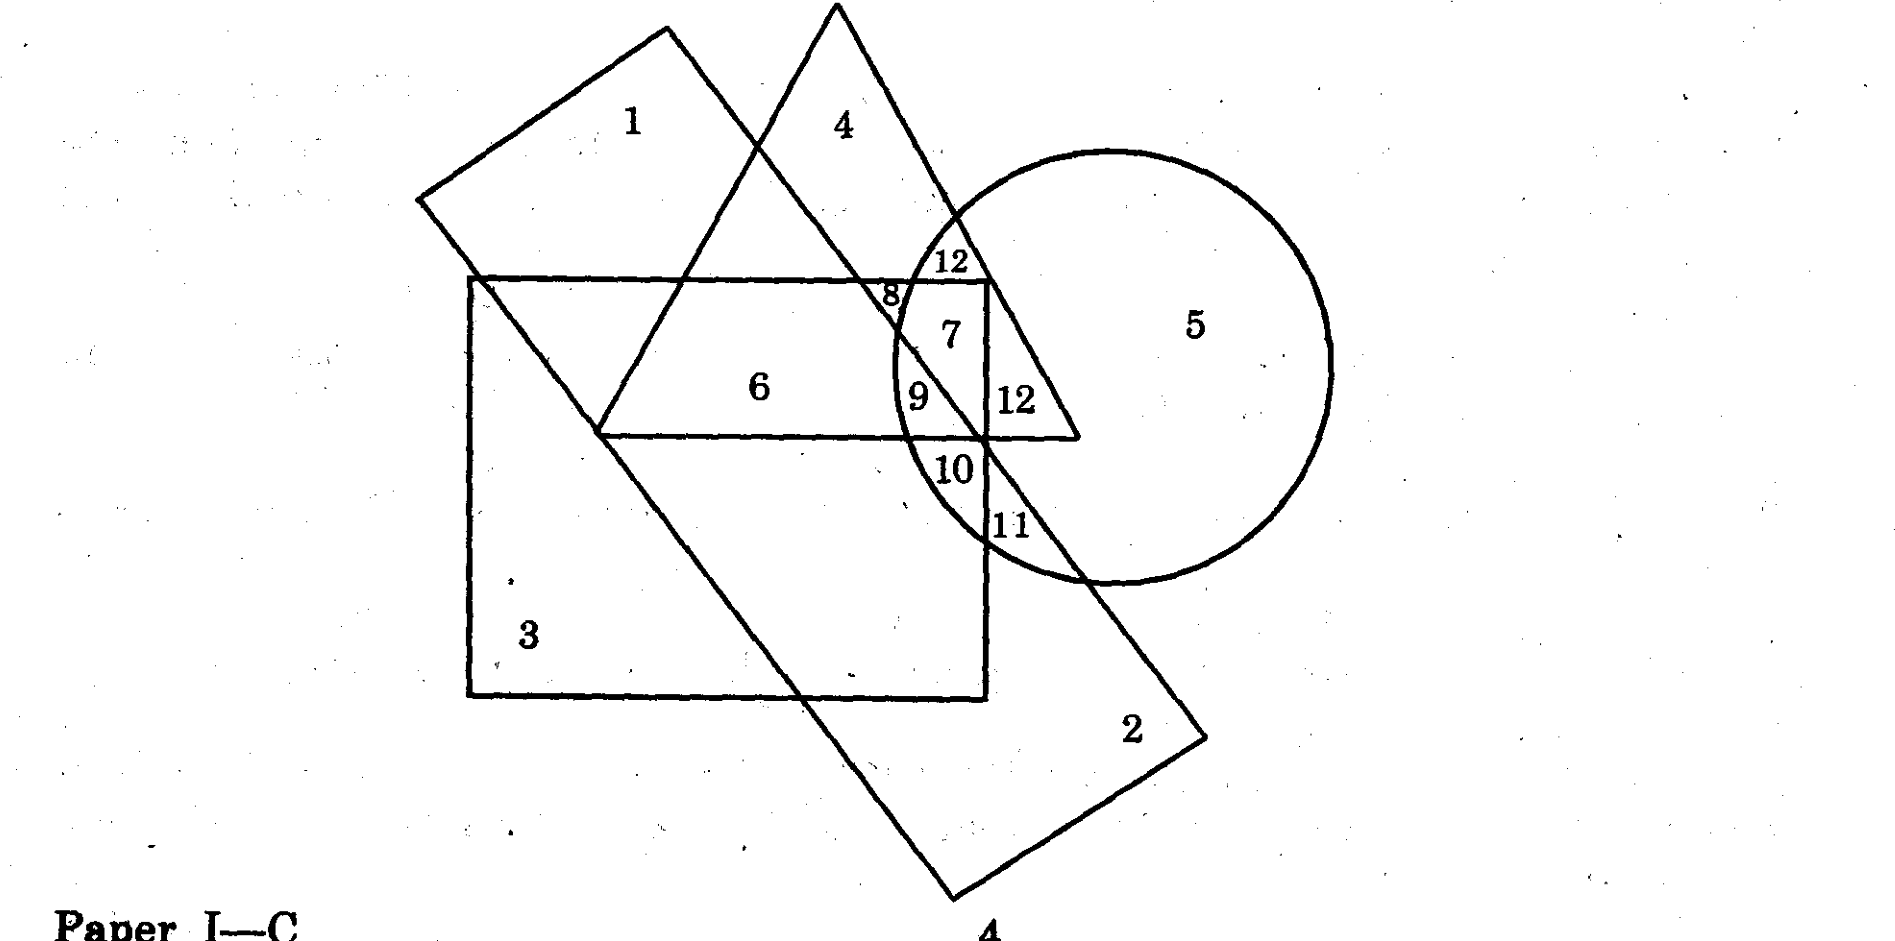
\includegraphics[width=0.72\linewidth]{fig/dec03_q6.png}\end{center}
\end{context}
\begin{question}{6}
{Non-rural and hardworking medical students who are affluent are represented by the region:\par}
\optsfour{5}{7}{9}{10}
\answer{D}{10}
\begin{explain}
Required: inside circle, square and tilted rectangle, but \textbf{outside the triangle}. That is region \textbf{10}.
\tip{Method for every such question: list the figures the region must be \emph{inside} and those it must be \emph{outside}, then find the single numbered region that satisfies all conditions.}
\end{explain}
\end{question}

\begin{question}{7}
{Medical students who are neither affluent nor hardworking but are rural are represented by the region :\par}
\optsfour{8}{10}{11}{12}
\answer{D}{12}
\begin{explain}
Inside circle and triangle; outside square and rectangle: region \textbf{12} (the part of the triangle inside the circle but above/right of the square and rectangle).
\end{explain}
\end{question}

\begin{question}{8}
{Hardworking, non-affluent rural medical students are represented by the region:\par}
\optsfour{6}{7}{9}{12}
\answer{B}{7}
\begin{explain}
Inside circle, square and triangle; outside the rectangle: region \textbf{7}.
\end{explain}
\end{question}

\begin{question}{9}
{Non-affluent medical students who are not hardworking and who do not belong to rural areas are represented by the region :\par}
\optsfour{5}{6}{8}{11}
\answer{A}{5}
\begin{explain}
Inside the circle only (outside square, triangle and rectangle): region \textbf{5}.
\end{explain}
\end{question}

\begin{question}{10}
{Medical students who are affluent, hardworking and rural are represented through the region:\par}
\optsfour{6}{8}{9}{10}
\answer{D}{10}
\begin{explain}
Inside all four figures (circle, square, triangle, rectangle): region \textbf{9}.
\end{explain}
\end{question}

\begin{question}{11}
{Complete the number series given below: 320, 320, 160, 40, ?\par}
\optsfour{4}{0}{5}{10}
\answer{C}{5}
\begin{explain}
Divide successively by 1, 2, 4, 8: $320\div1=320$, $\div2=160$, $\div4=40$, $\div8=\mathbf{5}$.
\end{explain}
\end{question}

\begin{question}{12}
{Complete the number series given below: 1, 5, 45, 445, ?\par}
\optsfour{4545}{4445}{5454}{4455}
\answer{B}{4445}
\begin{explain}
Each term $=$ previous $\times10-5$: $1\rightarrow5\rightarrow45\rightarrow445\rightarrow\mathbf{4445}$.
\end{explain}
\end{question}

\begin{question}{13}
{Which of the following will come next in the series given below: BHL, DJN, FLP, ?\par}
\optsfour{HNR}{HOS}{IOS}{INR}
\answer{A}{HNR}
\begin{explain}
Each letter advances by 2: B$\rightarrow$D$\rightarrow$F$\rightarrow$\textbf{H}, H$\rightarrow$J$\rightarrow$L$\rightarrow$\textbf{N}, L$\rightarrow$N$\rightarrow$P$\rightarrow$\textbf{R}. Next: \textbf{HNR}.
\end{explain}
\end{question}

\begin{question}{14}
{Which of the following will come next in the series given below: KUZ, MOX, OIV, QET, ?\par}
\optsfour{SUR}{SAQ}{RAR}{SAR}
\answer{C}{RAR}
\begin{explain}
First letters K, M, O, Q, \textbf{S} ($+2$); last letters Z, X, V, T, \textbf{R} ($-2$); middle letters U, O, I, E, \textbf{A} (moving back through the vowels). Next: \textbf{SAR}.
\end{explain}
\end{question}

\begin{question}{15}
{In the following letter sequence, find the correct alternative for the missing letters: ab.\ldots{}cba.\ldots{}bcc.\ldots{}aab.\ldots{}cba.\ldots{}b\par}
\optsfour{bbbba}{cabca}{caacb}{babcb}
\answer{B}{cabca}
\begin{explain}
Filling c, a, b, c, a gives
\[\text{ab\underline{c}cba\underline{a}bcc\underline{b}aab\underline{c}cba\underline{a}b}=\text{abccba}\,|\,\text{abccba}\,|\,\text{abccba}\,|\,\text{ab}\]
The block ``abccba'' repeats, so the answer is \textbf{cabca}.
\end{explain}
\end{question}

\begin{question}{16}
{In the following letter sequence, find the correct alternative for the missing letters: ab.\ldots{}abc.\ldots{}cab.\ldots{}bc.\ldots{}b\par}
\optsfour{cabcaa}{baabbc}{caaccc}{cachca}
\answer{A}{cabcaa}
\begin{explain}
Filling the gaps with c, a, b, c, a, a (option A) completes the repeating letter pattern built from ``abc''. Answer as per key: \textbf{cabcaa}.
\end{explain}
\end{question}

\begin{question}{17}
{A cube is painted red on two opposite faces and green on two adjacent faces. The remaining two faces are left uncoloured. It is cut into 125 equal cubes. How many cubes have green colour on one face only?\par}
\optsfour{16}{19}{24}{40}
\answer{C}{24}
\begin{explain}
The cube is cut $5\times5\times5$. Let top and bottom be red, front and right green, left and back uncoloured.
On the front (green) face, remove the top row and bottom row (also red) and the column on the right edge (also green): $3\times4=12$ cubes have green only. Same for the right face.
Total $=12\times2=\mathbf{24}$.
\end{explain}
\end{question}

\begin{question}{18}
{Referring to the cube described in Q17: How many cubes are coloured green on two faces ?\par}
\optsfour{2}{5}{7}{9}
\answer{B}{5}
\begin{explain}
Cubes with green on two faces lie along the common edge of the two green faces: $\mathbf{5}$ cubes (the two end cubes on this edge are also red, but they still carry green on two faces).
\end{explain}
\end{question}

\begin{question}{19}
{In the multiplication given below, find the digits corresponding to the letters:\\[3pt]
\centering\begin{tabular}{r} 6 b c\\ $\times$\ 3 5 d\\\hline 6 6 e\\ 3 3 3 0\ \ \\ 1 a a 8\ \ \ \ \\\hline 2 2 3 7 6 6\end{tabular}\\[3pt]
\raggedright `b' stands for:\par}
\optsfour{6}{7}{8}{9}
\answer{A}{6}
\begin{explain}
The second partial product is $6bc\times5=3330$, so $6bc=666$. Hence \textbf{b $=$ 6} (and c $=6$, d $=1$, e $=6$, a $=9$: $666\times3=1998$).
\end{explain}
\end{question}

\begin{question}{20}
{In the same multiplication, `c' stands for:\par}
\optsfour{7}{6}{5}{4}
\answer{B}{6}
\begin{explain}
From $6bc=666$ (because $6bc\times5=3330$): \textbf{c $=$ 6}.
\end{explain}
\end{question}

\begin{context}
\textbf{Q.~21--22:} A square cardboard ABCD, inside which the square JKLM is inscribed, is placed horizontally (and may be reversed). In each question, two conditions are given: (I) whether the cardboard is reversed; (II) the direction of one vertex with respect to the centre O. Find the direction of the other given vertex with respect to O.
\begin{center}
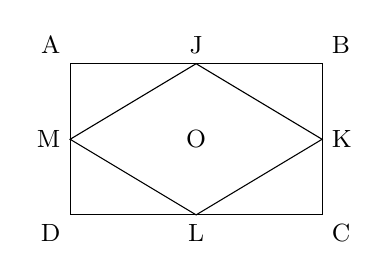
\begin{tikzpicture}[scale=0.8,font=\small]
\draw (0,0) rectangle (4,2.4); \draw (2,2.4)--(4,1.2)--(2,0)--(0,1.2)--cycle;
\node[above left] at (0,2.4){A}; \node[above right] at (4,2.4){B}; \node[below right] at (4,0){C}; \node[below left] at (0,0){D};
\node[above] at (2,2.4){J}; \node[right] at (4,1.2){K}; \node[below] at (2,0){L}; \node[left] at (0,1.2){M}; \node at (2,1.2){O};
\end{tikzpicture}
\end{center}
In the normal position: A $=$ NW, B $=$ NE, C $=$ SE, D $=$ SW; J $=$ N, K $=$ E, L $=$ S, M $=$ W.
\end{context}
\begin{question}{21}
{(I) Not reversed. (II) A towards S. `J' will be in the direction:\par}
\optsfour{N}{W}{SW}{NW}
\answer{C}{SW}
\begin{explain}
A moves from NW to S: a rotation of $225^\circ$ clockwise (NW $\rightarrow$ N $\rightarrow$ \ldots\ $\rightarrow$ S is 5 steps of $45^\circ$). J (N) rotated $225^\circ$ clockwise points \textbf{SW}.
\end{explain}
\end{question}

\begin{question}{22}
{(I) Not reversed. (II) L towards NE. `M' will be in the direction:\par}
\optsfour{SE}{E}{N}{S}
\answer{A}{SE}
\begin{explain}
L moves from S to NE: $225^\circ$ clockwise. M (W) rotated $225^\circ$ clockwise $\rightarrow$ \textbf{SE}.
\end{explain}
\end{question}

\begin{question}{23}
{Six persons I, II, III, IV, V and VI are sitting in a room. Three are females and three are males. I is father of III, III is son of II, III is brother of IV, IV is not son of I, V is nephew of I, VI is niece of II. Who is the daughter of I?\par}
\optsfour{IV}{VI}{III}{None of these}
\answer{B}{VI}
\keynote{By the given relations the daughter of I is IV. The official key gives (B) VI.}
\begin{explain}
I is father of III and II is mother (III is son of II). III is brother of IV, and IV is \emph{not} son of I, so IV is I's \textbf{daughter}. V and VI are nephew and niece (children of a sibling). Logically the answer is IV; the key gives \textbf{VI}.
\end{explain}
\end{question}

\begin{question}{24}
{If GOLD is coded as EMJB, then NMPR will be decoded as\par}
\optsfour{RIOT}{PORT}{ROTS}{PORK}
\answer{B}{PORT}
\begin{explain}
GOLD $\rightarrow$ EMJB: each letter moves 2 back. To decode NMPR, move each letter 2 forward: \textbf{PORT}.
\end{explain}
\end{question}

\begin{question}{25}
{If 6743 is coded as FGDC, then 97285 will be coded as:\par}
\optsfour{IGBHE}{RTYSV}{GVSTU}{IHCIF}
\answer{A}{IGBHE}
\begin{explain}
The code replaces digit $n$ by the $n$-th letter: 6$\rightarrow$F, 7$\rightarrow$G, 4$\rightarrow$D, 3$\rightarrow$C. So 97285 $\rightarrow$ I G B H E $=$ \textbf{IGBHE}.
\end{explain}
\end{question}

\begin{question}{26}
{At a certain restaurant, above the kitchen door four small lights, numbered 1 to 4 from left to right, are used to signal waiters: I $=$ all four lights; II $=$ lights 1 and 2; III $=$ light 1 only; IV $=$ lights 2, 3 and 4; V $=$ lights 3 and 4. Not-working lights are taken as illuminated.\\ If lights two and three both are off, then the waiter signalled could be:\par}
\optsfour{I}{II}{III}{IV}
\answer{C}{III}
\begin{explain}
With lights 2 and 3 off, only signals that do not use 2 or 3 remain: III (light 1 only). \textbf{III}.
\end{explain}
\end{question}

\begin{question}{27}
{If lights one and two are not working (and hence count as illuminated), and lights three and four are illuminated, then the signal of which of the waiters (I, IV and V) might be signalled?\par}
\optsfour{I only}{V only}{I and IV}{I, IV and V}
\answer{D}{I, IV and V}
\begin{explain}
Lights 3 and 4 are on and lights 1 and 2 may or may not be intended, so the signal could be I (all four), IV (2, 3, 4) or V (3, 4): \textbf{I, IV and V}.
\end{explain}
\end{question}

\begin{question}{28}
{Select from the following groups, the word that does not belong to the group:\par}
\optsfour{Tin}{Steel}{Iron}{Copper}
\answer{D}{Copper}
\keynote{Strictly, steel (an alloy) is the odd one out among the metallic elements tin, iron and copper. The official key gives (D) Copper.}
\begin{explain}
Tin, iron and copper are elements; steel is an alloy of iron. The official key, however, gives \textbf{Copper} (the only non-greyish, reddish metal of the group). Mark (D) as per the key.
\end{explain}
\end{question}

\begin{question}{29}
{Find the odd one out of the following:\par}
\optsfour{Truthful}{Sly}{Virtuous}{Pensive}
\answer{D}{Pensive}
\begin{explain}
Truthful, sly and virtuous describe a person's \emph{moral character}. \textbf{Pensive} (thoughtful) describes a \emph{mood}, so it is the odd one.
\end{explain}
\end{question}

\begin{question}{30}
{A watch costs Rs. 800. At what price should a shopkeeper mark up, if after allowing a discount of 10 per cent on the marked up price, he makes a profit of 12.5\% on the cost price ?\par}
\optsfour{Rs. 950}{Rs. 1,000}{Rs. 1,250}{Rs. 1,500}
\answer{B}{Rs. 1,000}
\begin{explain}
Required SP $=800\times1.125=900$. SP $=0.9\times$ MP, so MP $=900/0.9=$ \textbf{Rs.~1,000}.
\end{explain}
\end{question}

\begin{question}{31}
{In a college level instruction, the purpose of selective admission is to:\par}
\optsone{debar those who may create problem to the lecturer}{ensure equality and justice}{screen those who can benefit from higher education}{increase the revenue of the college through admission tests}
\answer{C}{screen those who can benefit from higher education}
\begin{explain}
Selective admission aims to \textbf{screen those who can benefit from higher education}, i.e.\ admit students with the required aptitude and preparation.
\end{explain}
\end{question}

\begin{question}{32}
{A lecturer is planning his/her lecture for a course. Which of the following may be considered least helpful?\par}
\optsone{deciding the content to be delivered}{identifying suitable methodology of presentation}{getting information about his/her students' background}{discussing with his/her principal as to what he/she considers to be the functions of a lecturer}
\answer{D}{discussing with his/her principal as to what he/she considers to be the functions of a lecturer}
\begin{explain}
Per the key, the least helpful step is option (D), discussing the plan with others. Deciding content, choosing methodology and knowing the students' background are essential parts of lecture planning.
\end{explain}
\end{question}

\begin{question}{33}
{During classroom teaching interactive sessions should be encouraged because :\par}
\optsone{teacher's job becomes less challenging during such sessions}{students' involvement is enhanced}{teaching is not everybody's cup of tea}{students should be given some breathing time to learn}
\answer{B}{students' involvement is enhanced}
\begin{explain}
Interactive sessions \textbf{enhance students' involvement}, which improves understanding and retention.
\end{explain}
\end{question}

\begin{question}{34}
{A college or a university should submit itself for evaluation to the National Assessment and Accreditation Council (NAAC) because :\par}
\optsone{It is the need of the hour}{It will enable it to know its strength and weaknesses}{It will justify its existence}{It will help in deciding grants for the college/university}
\answer{B}{It will enable it to know its strength and weaknesses}
\begin{explain}
NAAC evaluation helps an institution \textbf{know its strengths and weaknesses}, so that it can improve quality.
\end{explain}
\end{question}

\begin{question}{35}
{Which of the following pairs of incentives are likely to strongly motivate the adolescents ?\par}
\optstwo{Teacher and parents' approval}{Certificates and academic honours}{Peer and compeer approval}{Principal and teachers' encouragement}
\answer{C}{Peer and compeer approval}
\begin{explain}
Adolescents are strongly influenced by their peer group, so \textbf{peer and compeer approval} is the most powerful incentive.
\end{explain}
\end{question}

\begin{question}{36}
{The office of a Chief Proctor in a university has justification because :\par}
\optsone{There are a number of proctors in a university}{The university ordinance requires it to be so}{Students' activities/programmes need regulatory control}{Students are generally unruly and need control}
\answer{C}{Students' activities/programmes need regulatory control}
\begin{explain}
A Chief Proctor's office is justified because \textbf{students' activities and programmes need regulatory control} (discipline and order on campus).
\end{explain}
\end{question}

\begin{question}{37}
{Which research focusses on improvement of work situations ?\par}
\optstwo{Fundamental Research}{Applied Research}{Survey Research}{Action Research}
\answer{D}{Action Research}
\begin{explain}
\textbf{Action research} focuses on improving one's own work situation or practice.
\end{explain}
\end{question}

\begin{question}{38}
{The need for sampling in research arises because :\par}
\optstwo{It is economical}{It is time-saving}{It improves accuracy of results}{All the above considerations hold}
\answer{D}{All the above considerations hold}
\begin{explain}
Sampling is economical, saves time, and (because a smaller group can be studied more carefully) can improve accuracy: \textbf{all the above}.
\end{explain}
\end{question}

\begin{question}{39}
{A researcher has collected data in form of cross breaks by setting up a 2 x 3 table in terms of frequency counts. Which of the following tests will be most appropriate for arriving at an appropriate analysis ?\par}
\optsone{Parametric tests}{Non-parametric tests}{Both parametric and non-parametric tests}{Logical tests}
\answer{B}{Non-parametric tests}
\begin{explain}
Frequency counts in a $2\times3$ contingency table call for the \textbf{chi-square test}, a non-parametric test.
\end{explain}
\end{question}

\begin{question}{40}
{In reporting research findings the main purpose should be to:\par}
\optstwo{meet the sponsorer's expectations}{help other researchers}{attract public attention}{highlight the factual position}
\answer{D}{highlight the factual position}
\begin{explain}
The main purpose of reporting research is to \textbf{highlight the factual position}, i.e.\ to present the findings honestly and objectively.
\end{explain}
\end{question}

\begin{question}{41}
{Select the word that is the nearest equivalent to the capitalized word: ABDICATE :\par}
\optsfour{Plead}{Censure}{Renounce}{Abolish}
\answer{C}{Renounce}
\begin{explain}
\textbf{Abdicate} means to give up (a throne or responsibility), i.e.\ \textbf{renounce}.
\end{explain}
\end{question}

\begin{question}{42}
{Select the word that is the nearest equivalent to the capitalized word: SHAM:\par}
\optsfour{Lovable}{Pretence}{Guilty}{Jittery}
\answer{B}{Pretence}
\begin{explain}
\textbf{Sham} means something false or fake, i.e.\ \textbf{pretence}.
\end{explain}
\end{question}

\begin{question}{43}
{In arriving at knowledge through the method of research, which of the following combinations is most appropriate ?\par}
\optstwo{Authority + Inductive reasoning}{Experience + Deductive reasoning}{Creativity + Deductive reasoning}{Inductive + Deductive reasoning}
\answer{D}{Inductive + Deductive reasoning}
\begin{explain}
The research method combines \textbf{inductive and deductive reasoning} (the reflective or scientific method).
\end{explain}
\end{question}

\begin{question}{44}
{Select the lettered pair wherein the words have the closest relationship to that of the numbered pair: Information : Feedback ::\par}
\optstwo{Gun : Recoil}{Letter : Reply}{Action : Reaction}{Aborigines : Boomerang}
\answer{C}{Action : Reaction}
\begin{explain}
Feedback is the response that comes back to information. Similarly, reaction is the response to \textbf{action}.
\end{explain}
\end{question}

\begin{question}{45}
{Select the lettered pair wherein the words have the closest relationship to that of the numbered pair: Activate : Detonate ::\par}
\optstwo{Inform : Deform}{Engage : Disengage}{Quicken : Mutilate}{Deaden : Diffuse}
\answer{D}{Deaden : Diffuse}
\begin{explain}
Per the official key, the pair is \textbf{Deaden : Diffuse}, i.e.\ the second word is the (intensified) result of the first, as detonation follows activation.
\end{explain}
\end{question}

\begin{context}
\textbf{Q.~46--50:} Read the passage given below and answer the questions.\par\smallskip
Competition the world over is slowly becoming a lethal agent in killing the regenerative process among human beings. This is happening through a vicious cycle of anxiety--tension--stress--depression--nervous breakdown. The problem percolates to the entire human structure touching health of the body, mind and spirit. To prepare a sound mind in a sound body is a coveted definition of education. But in the present life-cycle dynamics everything seems to explode. More so for those aspiring to be competitive winners irrespective of the field, the killer instinct is soon becoming a self killing process. Much has been spoken and written about the evil effects of stress and its psychosomatic repercussions. Many solutions have been offered by counselling agencies across the globe --- some bordering on spiritual remedies, while large chunk depending upon psychiatric-psychic process. Many have also recommended physical activity to control stress and depression. However, an integrated approach to life management programme in the competitive environment could probably be the most easy and efficient course of remedy. But what is not clearly taken into reckoning is the fact that the body, the mind and the spirit all the three together form an individual and therefore, the health of each of these three components is equally important and has a separate existence. For instance, when the mind is disturbed, thereby creating unhealthiness in the intellectual-emotional plane, the body despite being in absolute physical comfort still gets affected and is often the victim. Therefore, it is necessary to understand fear and conquer it at the first place in order to arrest spread of anxiety, stress, tension and depression.
\end{context}
\begin{question}{46}
{Basic objective of this passage is to project:\par}
\optstwo{Ways of remaining healthy}{Avoidance of anxiety}{Avoidance of competitive spirit}{Causes of mental ill health}
\answer{D}{Causes of mental ill health}
\begin{explain}
The passage traces how competition produces anxiety, stress and depression and affects body, mind and spirit, i.e.\ the \textbf{causes of mental ill health}.
\end{explain}
\end{question}

\begin{question}{47}
{After going through this passage, two premises come up. You are to indicate which is right.\\
I. Anxiety leads to nervous breakdown.\\ II. Stress has evil effects on health.\par}
\optstwo{I is right and II is wrong}{I is wrong and II is right}{I and II both are right}{I and II both are wrong}
\answer{B}{I is wrong and II is right}
\begin{explain}
Per the key, only II is right: the passage directly states the ``evil effects of stress and its psychosomatic repercussions''. Anxiety is only the first link of a cycle, not directly said to cause breakdown.
\end{explain}
\end{question}

\begin{question}{48}
{The whole passage is structured in the form which may be called:\par}
\optsfour{Narrative}{Explanatory}{Analytical}{Expository}
\answer{B}{Explanatory}
\begin{explain}
The passage explains a problem, its causes and possible remedies, so it is \textbf{explanatory}.
\end{explain}
\end{question}

\begin{question}{49}
{The most appropriate title for the passage would be :\par}
\optstwo{Evil effects of competition}{Managing good health}{Overcoming stress}{Managing good living}
\answer{C}{Overcoming stress}
\begin{explain}
The passage ends with the need to understand fear and arrest stress, anxiety and depression, so the best title is \textbf{Overcoming Stress}.
\end{explain}
\end{question}

\begin{question}{50}
{In the passage the words 'Disturbed Mind' can be suitably replaced by the words:\par}
\optsfour{Activated Mind}{Agitated Mind}{Unhealthy Mind}{Anxious Mind}
\answer{B}{Agitated Mind}
\begin{explain}
A ``disturbed mind'' is an \textbf{agitated mind}.
\end{explain}
\end{question}

\paperchapter{December 2002}{1 December 2002}{B}{50}{GSET 2002 (II)}
\keytable{\kcell{1}{C} & \kcell{2}{A} & \kcell{3}{C} & \kcell{4}{C} & \kcell{5}{D} & \kcell{6}{D} & \kcell{7}{B} & \kcell{8}{B} & \kcell{9}{D} & \kcell{10}{B} \\
\kcell{11}{A} & \kcell{12}{C} & \kcell{13}{A} & \kcell{14}{D} & \kcell{15}{C} & \kcell{16}{B} & \kcell{17}{C} & \kcell{18}{A} & \kcell{19}{A} & \kcell{20}{D} \\
\kcell{21}{B} & \kcell{22}{C} & \kcell{23}{C} & \kcell{24}{B} & \kcell{25}{D} & \kcell{26}{C} & \kcell{27}{C} & \kcell{28}{A} & \kcell{29}{D} & \kcell{30}{B} \\
\kcell{31}{A} & \kcell{32}{B} & \kcell{33}{D} & \kcell{34}{C} & \kcell{35}{B} & \kcell{36}{C} & \kcell{37}{D} & \kcell{38}{A} & \kcell{39}{A} & \kcell{40}{C} \\
\kcell{41}{B} & \kcell{42}{D} & \kcell{43}{A} & \kcell{44}{B} & \kcell{45}{D} & \kcell{46}{B} & \kcell{47}{D} & \kcell{48}{C} & \kcell{49}{A} & \kcell{50}{B}}
\begin{question}{1}
{Complete the series: 1, 3, 4, 8, 16, ?\par}
\optsfour{30}{31}{32}{33}
\answer{C}{32}
\begin{explain}
Each term (from the third) is the \textbf{sum of all previous terms}: $1+3=4$, $1+3+4=8$, $1+3+4+8=16$, so next $=1+3+4+8+16=\mathbf{32}$.
\end{explain}
\end{question}

\begin{question}{2}
{Complete the series: 10, 12, 16, 22, 30, ?\par}
\optsfour{40}{50}{60}{70}
\answer{A}{40}
\begin{explain}
The differences are $2, 4, 6, 8$, so next $+10$: $30+10=\mathbf{40}$.
\end{explain}
\end{question}

\begin{question}{3}
{Complete the series: 240, 240, 120, 40, ?\par}
\optsfour{30}{20}{10}{0}
\answer{C}{10}
\begin{explain}
Divide successively by 1, 2, 3, 4: $240, 240, 120, 40, \mathbf{10}$.
\end{explain}
\end{question}

\begin{question}{4}
{If CENTRAL has been coded as XVMGIZO, what will be the correct code for PHYSICS?\par}
\optsfour{KSBRHHX}{HXBHKRX}{KSBHRXH}{HXRHSBK}
\answer{C}{KSBHRXH}
\begin{explain}
CENTRAL $\rightarrow$ XVMGIZO uses the \textbf{reverse-alphabet} code (A$\leftrightarrow$Z, B$\leftrightarrow$Y, C$\leftrightarrow$X, \ldots; the two letters add to 27).
PHYSICS: P$\rightarrow$K, H$\rightarrow$S, Y$\rightarrow$B, S$\rightarrow$H, I$\rightarrow$R, C$\rightarrow$X, S$\rightarrow$H, giving \textbf{KSBHRXH}.
\end{explain}
\end{question}

\begin{question}{5}
{If GOAT is coded as HPBU, what will be the correct code for LIME ?\par}
\optsfour{ORNZ}{MJND}{KHLF}{MJNF}
\answer{D}{MJNF}
\begin{explain}
Each letter moves one step forward (G$\rightarrow$H, O$\rightarrow$P, \ldots). LIME $\rightarrow$ \textbf{MJNF}.
\end{explain}
\end{question}

\begin{question}{6}
{If CHEMISTRY has been coded as DGFLJRUQZ, what will be the correct code for DESIGN?\par}
\optsfour{EDTHMN}{EDTMHN}{EDTHNN}{EDTHHM}
\answer{D}{EDTHHM}
\begin{explain}
CHEMISTRY $\rightarrow$ DGFLJRUQZ: the shifts alternate $+1, -1$.
DESIGN: D$+1=$E, E$-1=$D, S$+1=$T, I$-1=$H, G$+1=$H, N$-1=$M, giving \textbf{EDTHHM}.
\end{explain}
\end{question}

\begin{question}{7}
{If CARPET is coded as XZIKVG, what will be the correct code for MARKET?\par}
\optsfour{NZIPUG}{NZIPVG}{NZIQVG}{NZIPTG}
\answer{B}{NZIPVG}
\begin{explain}
CARPET $\rightarrow$ XZIKVG is again the reverse-alphabet code. MARKET $\rightarrow$ N, Z, I, P, V, G $=$ \textbf{NZIPVG}.
\end{explain}
\end{question}

\begin{question}{8}
{The quality of research is judged by the:\par}
\optsone{Relevance of research}{Methodology followed in conducting the research}{Depth of the research}{Experience of the researcher}
\answer{B}{Methodology followed in conducting the research}
\begin{explain}
The quality of research is judged mainly by the \textbf{methodology} followed: the rigour of design, sampling, tools and analysis determines the validity of the findings.
\end{explain}
\end{question}

\begin{question}{9}
{Which one of the following statements is not correct?\par}
\optstwo{Any person can do research.}{Research may be without a hypothesis.}{Research requires library facilities.}{Research is not always systematic.}
\answer{D}{Research is not always systematic.}
\begin{explain}
Research is by definition a \emph{systematic} inquiry. So ``research is not always systematic'' is \textbf{not correct}.
\end{explain}
\end{question}

\begin{question}{10}
{The first step of research is:\par}
\optstwo{Selection of Problem}{Identification of Problem}{Definition of Problem}{Locating the Problem}
\answer{B}{Identification of Problem}
\begin{explain}
The first step is \textbf{identification of the problem}; selection and definition follow.
\end{explain}
\end{question}

\begin{question}{11}
{A good researcher must possess:\par}
\optstwo{an inquiry mind}{a master's degree}{a good health}{enough funds}
\answer{A}{an inquiry mind}
\begin{explain}
A good researcher must above all possess an \textbf{inquiring mind} (curiosity).
\end{explain}
\end{question}

\begin{question}{12}
{Which one of the following statements is not correct?\par}
\optsone{Hypothesis and assumptions are not same.}{Problem refers to variable.}{Quantitative data can be converted into qualitative data.}{Qualitative data may be converted into quantitative data.}
\answer{C}{Quantitative data can be converted into qualitative data.}
\begin{explain}
Per the key, ``quantitative data can be converted into qualitative data'' is treated as \textbf{not correct}. Statement (D), converting qualitative data into quantitative data by coding and counting, is common practice.
\end{explain}
\end{question}

\begin{context}
\textbf{Read the following passage and answer the questions 13--16.}\par\smallskip
Both plants and animals of many sorts show remarkable changes in form, structure, growth habits, and even mode of reproduction in becoming adapted to different climatic environment, types of food supply, or mode of living. This divergence in response to evolution is commonly expressed by altering the form and function of some part or parts of the organism, the original identity of which is clearly discernible. For example, the creeping foot of the snail is seen in related marine pteropods to be modified into a flapping organ useful for swimming, and is changed into prehensile arms that bear suctorial disks in the squids and other cephalopods. The limbs of various mammals are modified according to several different modes of life-for swift running (cursorial) as in the horse and antelope, for swinging in trees (arboreal) as in the monkeys, for digging (fossorial) as in the moles and gophers, for flying (volant) as in the bats, for swimming (aquatic) as in the seals, whales and dolphins, and for other adaptations. The structures or organs that show main change in connection with this adaptive divergence are commonly identified readily as homologous, in spite of great alterations. Thus, the finger and wristbones of a bat and whale, for instance, have virtually nothing in common except that they are definitely equivalent elements of the mammalian limb.
\end{context}
\begin{question}{13}
{Which of the following is the most appropriate title for the passage, based on its content ?\par}
\optstwo{Adaptive Divergence}{Evolution}{Changes in Organs}{Our Changing Bodies}
\answer{A}{Adaptive Divergence}
\begin{explain}
The passage describes how organisms diverge in form in \emph{adapting} to different environments: \textbf{Adaptive Divergence} (the term the passage itself uses).
\end{explain}
\end{question}

\begin{question}{14}
{The author provides information that would answer which of the following questions?\newline (I) What factors cause change in organisms ?\newline (II) What is the theory of evolution?\newline (III) How are horses' legs related to seals' flippers ?\par}
\optsfour{I only}{II only}{I and II only}{I and III only}
\answer{D}{I and III only}
\begin{explain}
The passage explains that climate, food supply and mode of living cause change (I), and it relates the limbs of horses (running) and seals (swimming) as homologous (III). It does not explain the theory of evolution (II). \textbf{I and III only}.
\end{explain}
\end{question}

\begin{question}{15}
{Which of the following words could best be substituted for 'homologous' without substantially changing the author's meaning?\par}
\optsfour{Altered}{Mammalian}{Corresponding}{Divergent}
\answer{C}{Corresponding}
\begin{explain}
\textbf{Homologous} organs are equivalent or \textbf{corresponding} parts that share an origin despite different functions.
\end{explain}
\end{question}

\begin{question}{16}
{The author's style can best be described as:\par}
\optsfour{Humorous}{Objective}{Esoteric}{Patronizing}
\answer{B}{Objective}
\begin{explain}
The author presents facts and examples without personal bias: an \textbf{objective} style.
\end{explain}
\end{question}

\begin{context}
\textbf{Read the following passage and answer the questions 17--22.}\par\smallskip
The atmosphere is a mixture of several gases. There are about ten chemical elements which remain permanently in gaseous form in the atmosphere under all natural conditions. Of these permanent gases, oxygen makes up about 21 percent and nitrogen about 78 percent. Several other gases, such as argon, carbon dioxide, hydrogen, neon, krypton and Xenon, comprise the remaining 1 percent of the volume of dry air. The amount of water vapour, and its variations in amount and distribution, are of extraordinary importance in weather changes. Atmospheric gases hold in suspension great quantities of dust, pollen, smoke and other impurities which are always present in considerable, but variable amounts.

The atmosphere has no definite upper limits but gradually thins until it becomes imperceptible. Until recently it was assumed that the air above the first few miles gradually grew thinner and colder at a constant rate. It was also assumed that upper air had little influence on weather changes. Recent studies of the upper atmosphere, currently being conducted by earth satellites and missile probings, have shown these assumptions to be incorrect. The atmosphere has three well-defined strata.

The layer of the air next to the earth, which extends upward for about 10 miles, is known as troposphere. On the whole, it makes up about 75 percent of all the weight of the atmosphere. It is the warmest part of the atmosphere because most of the solar radiation is absorbed by the earth's surface, which warms the air immediately surrounding it. A steady decrease of temperature with increasing elevation is a most striking characteristic. The upper layers are colder because of their great distance from the earth's surface and rapid radiation of heat into space. The temperatures within the troposphere decrease about 3.5 degrees per 1,000 foot increase in altitude. Within the troposphere, winds and air currents distribute heat and moisture. Strong winds, called jet streams, are located at the upper levels of the troposphere. These jet streams are both complex and wide spread in occurrence. They normally show a wave-shaped pattern and move from west to east at velocities of 150 mph, but velocities as high as 400 mph have been noted. The influences of changing locations and strengths of jet streams upon weather conditions and patterns are no doubt considerable. Current intensive research may eventually reveal their true significance.

Above the troposphere to a height of about 50 miles is a zone called the stratosphere. The stratosphere is separated from the troposphere by a zone of uniform temperatures called tropopause. Within the lower portions of the stratosphere is a layer of ozone gases which filters outmost of the ultraviolet rays from the sun. The ozone layer varies with air pressure. If this zone was not there, the full blast of the sun's ultraviolet light would burn our skin, blind our eyes, and eventually result in our destruction. Within the stratosphere, the temperature and atmospheric composition are relatively uniform.

The layer upward of about 50 miles is the most fascinating but the least known of these three strata. It is called ionosphere because it consists of electrically charged particles called ions, thrown from the sun. The northern lights (aurora borealis) originate within this highly charged portion of the atmosphere. Its effect upon weather conditions, if any, is as yet unknown.
\end{context}
\begin{question}{17}
{Which of the following titles best summarizes the content of the passage?\par}
\optsone{New methods for calculating the composition of the Atmosphere}{New Evidence concerning the stratification of the Atmosphere}{The Atmosphere: Its nature and importance to our weather}{The underlying causes of Atmospheric Turbulence}
\answer{C}{The Atmosphere: Its nature and importance to our weather}
\begin{explain}
The passage describes the composition and layers of the atmosphere and repeatedly relates them to weather: \textbf{The Atmosphere: its nature and importance to our weather}.
\end{explain}
\end{question}

\begin{question}{18}
{According to the passage, life as we know it exists on the earth because the atmosphere:\par}
\optsone{contains a layer of ozone gases.}{contains electrically charged particles.}{is warmest at the bottom.}{carries the ultraviolet rays of the sun.}
\answer{A}{contains a layer of ozone gases.}
\begin{explain}
The \textbf{ozone layer} filters the Sun's ultraviolet rays; without it ``the full blast of the sun's ultraviolet light would \ldots\ result in our destruction''.
\end{explain}
\end{question}

\begin{question}{19}
{The passage supplies information that would answer which of the following questions ?\newline (I) How do the troposphere and the stratosphere differ ?\newline (II) How does the ionosphere affect the weather?\newline (III) How do earth satellites study the atmosphere ?\par}
\optsfour{I only}{II only}{III only}{I, II and III}
\answer{A}{I only}
\begin{explain}
Only question I is answered (the troposphere and stratosphere are contrasted in temperature and composition). The ionosphere's effect on weather is ``as yet unknown'' (II), and how satellites study the atmosphere is not explained (III). \textbf{I only}.
\end{explain}
\end{question}

\begin{question}{20}
{The passage states that the troposphere is the warmest part of the atmosphere because it :\par}
\optsone{is the closest to the sun.}{radiates heat into space.}{has winds and air current that distribute the heat.}{is warmed by the earth's heat.}
\answer{D}{is warmed by the earth's heat.}
\begin{explain}
The troposphere is warmest ``because most of the solar radiation is absorbed by the earth's surface, which warms the air immediately surrounding it'', i.e.\ it is \textbf{warmed by the earth's heat}.
\end{explain}
\end{question}

\begin{question}{21}
{According to the passage, the atmosphere consists of all of the following, except:\par}
\optstwo{21 percent oxygen}{a definite amount of water vapour}{ten permanent elements}{considerable waste products}
\answer{B}{a definite amount of water vapour}
\begin{explain}
The passage stresses the \emph{variations} in the amount of water vapour, so ``a \textbf{definite} amount of water vapour'' is the exception.
\end{explain}
\end{question}

\begin{question}{22}
{It can be inferred from the passage that at the top of Jungfrau, which is 12,000 feet above the town of Interlaken in Switzerland, the temperature is usually :\par}
\optsone{below freezing}{warmer than in Interlaken}{about 42 degrees colder than on the ground}{about 75 degrees colder than in Interlaken}
\answer{C}{about 42 degrees colder than on the ground}
\begin{explain}
Temperature falls about $3.5^\circ$ per 1,000 ft, so at 12,000 ft: $12\times3.5=\mathbf{42}^\circ$ colder than on the ground.
\end{explain}
\end{question}

\begin{question}{23}
{If I say 'sky is down and winter is hot', I would call a criminal:\par}
\optsfour{Gangster}{A cloud}{Saint}{Delinquent}
\answer{C}{Saint}
\begin{explain}
The speaker uses words in their \emph{opposite} sense (sky is ``down'', winter is ``hot''), so a criminal would be called a \textbf{saint}.
\end{explain}
\end{question}

\begin{question}{24}
{If Dolly's mother is John's father's sister, what relation is John to Dolly's father ?\par}
\optsfour{Cousin}{Nephew}{Uncle}{Brother}
\answer{B}{Nephew}
\begin{explain}
Dolly's mother is John's paternal aunt, so Dolly's father is the husband of John's aunt, i.e.\ John's uncle (by marriage). John is his \textbf{nephew}.
\end{explain}
\end{question}

\begin{question}{25}
{Establish the relationship between the first two items. Find out the same relationship among the choices which follow the pattern of the two items: 20:21:: ?\par}
\optsfour{6:10}{10:B}{S: V}{A: B}
\answer{D}{A: B}
\begin{explain}
20 : 21 are consecutive numbers, corresponding to T : U, consecutive letters. Similarly \textbf{A : B} are consecutive (positions 1, 2).
\end{explain}
\end{question}

\begin{context}
\textbf{Study the pie-chart and answer the questions 26 to 30.} (The percentages below are those implied by the questions and official answers; the original chart was printed without values.)
\begin{center}
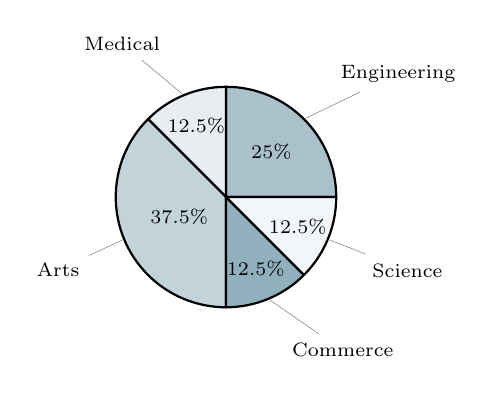
\begin{tikzpicture}\pie[radius=1.4,text=pin,font=\scriptsize,color={brand!35,brand!10,brand!25,brand!45,brand!5}]{25/Engineering,12.5/Medical,37.5/Arts,12.5/Commerce,12.5/Science}\end{tikzpicture}
\end{center}
\end{context}
\begin{question}{26}
{What is the percentage of total students enrolled in Medical and Engineering faculties ?\par}
\optsfour{33.50}{50.50}{37.50}{25.50}
\answer{C}{37.50}
\begin{explain}
Medical $+$ Engineering $=12.5\%+25\%=\mathbf{37.5\%}$.
\end{explain}
\end{question}

\begin{question}{27}
{What is the percentage of students enrolled in Arts and Science faculties?\par}
\optsfour{90}{60}{50}{45}
\answer{C}{50}
\begin{explain}
Arts $+$ Science $=37.5\%+12.5\%=\mathbf{50\%}$.
\end{explain}
\end{question}

\begin{question}{28}
{What is the percentage of students enrolled in Arts and Engineering faculties ?\par}
\optsfour{62.50}{75.00}{50.50}{33.33}
\answer{A}{62.50}
\begin{explain}
Arts $+$ Engineering $=37.5\%+25\%=\mathbf{62.5\%}$.
\end{explain}
\end{question}

\begin{question}{29}
{Suppose that the number of students enrolled in Engineering is 320; what is the number of students enrolled in Arts faculty?\par}
\optsfour{450}{460}{470}{480}
\answer{D}{480}
\begin{explain}
Engineering $=25\%=320$, so $1\%=12.8$ and Arts $=37.5\%=37.5\times12.8=\mathbf{480}$.
\end{explain}
\end{question}

\begin{question}{30}
{Suppose, the number of students enrolled in Engineering is 320; what is the total number of students enrolled in Commerce, Arts and Medical faculties?\par}
\optsfour{700}{800}{900}{1000}
\answer{B}{800}
\begin{explain}
Commerce $+$ Arts $+$ Medical $=12.5+37.5+12.5=62.5\%$ of $1280=\mathbf{800}$.
\end{explain}
\end{question}

\begin{question}{31}
{All streets are watches. All watches are eagles. Therefore :\newline (I) All streets are eagles.\newline (II) All watches are streets.\par}
\optstwo{if only inference (I) follows}{if only inference (II) follows}{if both of them follow}{if neither of them follows}
\answer{A}{if only inference (I) follows}
\begin{explain}
\begin{center}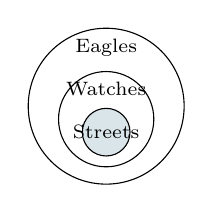
\begin{tikzpicture}[scale=0.55,font=\scriptsize]\draw (0,0) circle(1.8); \node at (0,1.35){Eagles}; \draw (0,-0.3) circle(1.1); \node at (0,0.4){Watches}; \draw[fill=brand!15] (0,-0.6) circle(0.55) node{Streets};\end{tikzpicture}\end{center}
All streets are watches and all watches are eagles, so \textbf{all streets are eagles} (I follows). II (all watches are streets) is the illicit converse. \textbf{Only I}.
\end{explain}
\end{question}

\begin{question}{32}
{All boys are mothers. All mothers are father. Therefore :\newline (I) All mothers are boys.\newline (II) All boys are fathers.\par}
\optstwo{if only inference (I) follows}{if only inference (II) follows}{if both of them follow}{if neither of them follows}
\answer{B}{if only inference (II) follows}
\begin{explain}
All boys are mothers and all mothers are fathers, so \textbf{all boys are fathers} (II follows). I (all mothers are boys) is an illicit converse. \textbf{Only II}.
\end{explain}
\end{question}

\begin{question}{33}
{Monkey is a bird. Some birds are clouds. Therefore :\newline (I) Monkey is a cloud.\newline (II) Some clouds are birds.\par}
\optstwo{if only inference (I) follows}{if only inference (II) follows}{if both of them follow}{if neither of them follows}
\answer{D}{if neither of them follows}
\keynote{Strictly, ``Some birds are clouds'' converts validly to ``Some clouds are birds'', so II follows. The official key gives (D).}
\begin{explain}
``Monkey is a bird'' and ``some birds are clouds'' do not show that the monkey is among those birds that are clouds, so I does not follow. II is the simple converse of the second premise. The official key, however, gives \textbf{neither follows}.
\end{explain}
\end{question}

\begin{context}
Expected (E) as well as actual (A) increase in export of different items are given in the following table (values in crores). Take into account the proportions of expected and actual export.
\begin{center}\small
\begin{tabular}{l*{8}{c}}\toprule
& \multicolumn{2}{c}{1990} & \multicolumn{2}{c}{1991} & \multicolumn{2}{c}{1992} & \multicolumn{2}{c}{1993}\\\cmidrule(lr){2-3}\cmidrule(lr){4-5}\cmidrule(lr){6-7}\cmidrule(lr){8-9}
\textbf{Items} & E & A & E & A & E & A & E & A\\\midrule
Rice & 90 & 60 & 120 & 60 & 150 & 60 & 200 & 60\\ Sugar & 100 & 70 & 200 & 140 & 300 & 210 & 400 & 280\\ Wheat & 100 & 75 & 200 & 150 & 300 & 200 & 400 & 300\\ Textile & 500 & 450 & 700 & 600 & 800 & 700 & 1000 & 850\\ Machinery & 1000 & 600 & 1500 & 700 & 2000 & 1500 & 2500 & 1500\\ Electronic goods & 1500 & 1200 & 2000 & 1500 & 2500 & 2000 & 3000 & 2000\\\bottomrule
\end{tabular}\\[4pt]
\textbf{Actual as \% of expected:}\\[2pt]
\begin{tabular}{lcccc}\toprule & 1990 & 1991 & 1992 & 1993\\\midrule
Rice & 66.7 & 50.0 & 40.0 & 30.0\\ Sugar & 70.0 & 70.0 & 70.0 & 70.0\\ Wheat & 75.0 & 75.0 & 66.7 & 75.0\\ Textile & 90.0 & 85.7 & 87.5 & 85.0\\ Machinery & 60.0 & 46.7 & 75.0 & 60.0\\ Electronic goods & 80.0 & 75.0 & 80.0 & 66.7\\\bottomrule
\end{tabular}
\end{center}
\end{context}
\begin{question}{34}
{Which item indicates consistent decrease in the export during the four years ?\par}
\optstwo{Electronic goods}{Textile}{Rice}{Sugar}
\answer{C}{Rice}
\begin{explain}
Only \textbf{rice} falls every year: 66.7\% $\rightarrow$ 50\% $\rightarrow$ 40\% $\rightarrow$ 30\%.
\end{explain}
\end{question}

\begin{question}{35}
{During 1990 which one of the four items had the highest percentage of export (Actual/Expected) ?\par}
\optsfour{Machinery}{Textile}{Wheat}{Sugar}
\answer{B}{Textile}
\begin{explain}
In 1990: Machinery 60\%, \textbf{Textile 90\%}, Wheat 75\%, Sugar 70\%. Textile is highest.
\end{explain}
\end{question}

\begin{question}{36}
{During which year the percent export of wheat was the lowest ?\par}
\optsfour{1990}{1991}{1992}{1993}
\answer{C}{1992}
\begin{explain}
Wheat: 75, 75, \textbf{66.7}, 75. The lowest is \textbf{1992}.
\end{explain}
\end{question}

\begin{question}{37}
{In which year sugar export was the lowest ?\par}
\optsfour{1990}{1992}{1993}{None of these}
\answer{D}{None of these}
\begin{explain}
Sugar's percentage is 70\% in every year, so there is no single lowest year: \textbf{none of these}.
\end{explain}
\end{question}

\begin{question}{38}
{During 1993 which item has the lowest percentage of export ?\par}
\optsfour{Rice}{Sugar}{Wheat}{Machinery}
\answer{A}{Rice}
\begin{explain}
1993: \textbf{Rice 30\%}, Sugar 70\%, Wheat 75\%, Machinery 60\%. Rice is lowest.
\end{explain}
\end{question}

\begin{question}{39}
{Which word does not belong to the other three ?\par}
\optsfour{Think}{See}{Hear}{Smell}
\answer{A}{Think}
\begin{explain}
See, hear and smell are \emph{sense perceptions}; \textbf{think} is a mental (cognitive) process.
\end{explain}
\end{question}

\begin{question}{40}
{Find one group of letters which is different from the other three:\par}
\optsfour{TRP}{SQO}{TVX}{YWU}
\answer{C}{TVX}
\begin{explain}
TRP, SQO and YWU move backwards in steps of 2; \textbf{TVX} moves forwards, so it is different.
\end{explain}
\end{question}

\begin{question}{41}
{Teaching refers to:\par}
\optsone{giving information related to the subject.}{creating environment that is conducive for learning.}{dictating notes in the classroom.}{solving difficulties of students related to the subject.}
\answer{B}{creating environment that is conducive for learning.}
\begin{explain}
Teaching means \textbf{creating an environment conducive to learning}, not merely giving information or dictating notes.
\end{explain}
\end{question}

\begin{question}{42}
{Which one of the following statements in not true?\par}
\optsone{Majority of teachers use lecture method.}{The lecture method is less structured.}{Lecture method is the best for giving more information in less time.}{There are well-defined steps of lecture method.}
\answer{D}{There are well-defined steps of lecture method.}
\begin{explain}
Per the key, the untrue statement is (D). The lecture method is widely used, fairly structured and efficient for conveying information; statement (D) overstates its standing.
\end{explain}
\end{question}

\begin{question}{43}
{Good teaching is best reflected by:\par}
\optsone{meaningful questions asked by students.}{attendance of students.}{number of distinctions.}{pin-drop silence in the class.}
\answer{A}{meaningful questions asked by students.}
\begin{explain}
Good teaching is reflected in the \textbf{meaningful questions asked by students}, which show understanding and curiosity.
\end{explain}
\end{question}

\begin{question}{44}
{The main objective of teaching at higher education level is:\par}
\optsone{to give information.}{to develop reasoning and thinking abilities.}{to develop expression power.}{to develop study habits.}
\answer{B}{to develop reasoning and thinking abilities.}
\begin{explain}
The main objective of higher education teaching is to \textbf{develop reasoning and thinking abilities}.
\end{explain}
\end{question}

\begin{question}{45}
{Noise in the classroom is best indicative of:\par}
\optsone{Only interaction among students.}{Only interaction among teacher and students.}{Only interaction between teacher and student.}{(A) and/or (B).}
\answer{D}{(A) and/or (B).}
\begin{explain}
Noise in class may come from interaction among students \emph{and/or} between teacher and students: \textbf{(A) and/or (B)}.
\end{explain}
\end{question}

\begin{question}{46}
{A student is reading a book at home. In this situation :\par}
\optsone{There is no communication.}{There is a communication.}{There is a two-way communication.}{There is only non-verbal communication.}
\answer{B}{There is a communication.}
\begin{explain}
Reading a book is communication between the author (sender) and the reader (receiver) through the printed text (channel): \textbf{there is communication} (one-way).
\end{explain}
\end{question}

\begin{question}{47}
{The facial expressions of students relate to which element of the communication process?\par}
\optsfour{Message}{Receiver}{Sender}{Channel}
\answer{D}{Channel}
\begin{explain}
Facial expressions are a \textbf{non-verbal channel} through which students send messages (interest, confusion, boredom) back to the teacher. The key therefore relates them to the \textbf{channel} of communication.
\end{explain}
\end{question}

\begin{question}{48}
{Communication refers to:\par}
\optsone{exchange of information only.}{exchange of feelings only.}{exchange of information, feelings, emotions and views.}{exchange of emotions only.}
\answer{C}{exchange of information, feelings, emotions and views.}
\begin{explain}
Communication is the \textbf{exchange of information, feelings, emotions and views}.
\end{explain}
\end{question}

\begin{question}{49}
{The Indian classrooms are generally best characterised by:\par}
\optstwo{One-way verbal communication}{Two-way verbal communication}{One-way communication}{Verbal communication}
\answer{A}{One-way verbal communication}
\begin{explain}
Indian classrooms are typically dominated by the lecture: \textbf{one-way verbal communication}.
\end{explain}
\end{question}

\begin{question}{50}
{Two persons sitting facing each other are engrossed in thinking. In this situation:\par}
\optsone{There is non-verbal communication.}{There is no communication.}{There is two-way non-verbal communication.}{There is less verbal communication.}
\answer{B}{There is no communication.}
\begin{explain}
Two people engrossed in their own thoughts are not exchanging any message, so there is \textbf{no communication} between them.
\end{explain}
\end{question}

\paperchapter{January 2002}{20 January 2002}{B}{50}{GSET 2002 (I)}
\keytable{\kcell{1}{A} & \kcell{2}{D} & \kcell{3}{D} & \kcell{4}{D} & \kcell{5}{C} & \kcell{6}{D} & \kcell{7}{C} & \kcell{8}{D} & \kcell{9}{C} & \kcell{10}{A} \\
\kcell{11}{C} & \kcell{12}{C} & \kcell{13}{B} & \kcell{14}{C} & \kcell{15}{D} & \kcell{16}{D} & \kcell{17}{B} & \kcell{18}{B} & \kcell{19}{D} & \kcell{20}{C} \\
\kcell{21}{D} & \kcell{22}{B} & \kcell{23}{C} & \kcell{24}{A} & \kcell{25}{A} & \kcell{26}{C} & \kcell{27}{A} & \kcell{28}{B} & \kcell{29}{B} & \kcell{30}{D} \\
\kcell{31}{C} & \kcell{32}{C} & \kcell{33}{A} & \kcell{34}{A} & \kcell{35}{D} & \kcell{36}{A} & \kcell{37}{A} & \kcell{38}{D} & \kcell{39}{B} & \kcell{40}{A} \\
\kcell{41}{D} & \kcell{42}{B} & \kcell{43}{B} & \kcell{44}{B} & \kcell{45}{D} & \kcell{46}{C} & \kcell{47}{C} & \kcell{48}{A} & \kcell{49}{C} & \kcell{50}{B}}
\begin{question}{1}
{Doctor and patient have same relationship as:\par}
\optstwo{Teacher and student}{Library and books}{Class and learning}{Husband and wife}
\answer{A}{Teacher and student}
\begin{explain}
A doctor serves and treats a patient; a \textbf{teacher} serves and teaches a \textbf{student}. The relationship is \emph{professional : the person served}.
\end{explain}
\end{question}

\begin{question}{2}
{Which one is different from the rest three ?\par}
\optsfour{Apple}{Orange}{Banana}{Fruit}
\answer{D}{Fruit}
\begin{explain}
Apple, orange and banana are \emph{kinds} of fruit; \textbf{fruit} is the general class, so it is different.
\end{explain}
\end{question}

\begin{question}{3}
{ACFJ: OUBJ:: SUXB: ?\par}
\optsfour{GNSA}{GLQZ}{GKPY}{GMTB}
\answer{D}{GMTB}
\begin{explain}
ACFJ: A(1), C(3), F(6), J(10), with gaps $+2, +3, +4$. OUBJ continues the same letters: O(15, $+5$), U(21, $+6$), B(28$\to$2, $+7$), J(10, $+8$). So the second group continues the first.
SUXB: S(19), U(21), X(24), B(28$\to$2). Continue: G(7, $+5$), M(13, $+6$), T(20, $+7$), B(28$\to$2, $+8$), giving \textbf{GMTB}.
\end{explain}
\end{question}

\begin{question}{4}
{BEAT: GIDV:: SOUP: ?\par}
\optsfour{XSYS}{YSXR}{YXSR}{XSXR}
\answer{D}{XSXR}
\begin{explain}
BEAT $\rightarrow$ GIDV: B$+5$, E$+4$, A$+3$, T$+2$.
SOUP $\rightarrow$ S$+5=$X, O$+4=$S, U$+3=$X, P$+2=$R, giving \textbf{XSXR}.
\end{explain}
\end{question}

\begin{question}{5}
{Which is the most effective method to control noise in a classroom?\par}
\optsone{Raising your voice above the students voice}{Saying 'don't talk'}{Remaining calm and just looking at students}{Continue teaching the class}
\answer{C}{Remaining calm and just looking at students}
\begin{explain}
Remaining calm and \textbf{silently looking at the students} usually restores order without confrontation. Shouting or scolding adds to the noise.
\end{explain}
\end{question}

\begin{question}{6}
{Choose one of the following statements as the most comprehensive way to define the job of a teacher:\par}
\optsone{Propagation of knowledge}{Conducting research}{Community service}{Propagation of knowledge, collection of knowledge and creation of knowledge}
\answer{D}{Propagation of knowledge, collection of knowledge and creation of knowledge}
\begin{explain}
A teacher's job comprises \textbf{propagation, collection (preservation) and creation of knowledge}, i.e.\ teaching, scholarship and research together.
\end{explain}
\end{question}

\begin{question}{7}
{A good academic researcher is:\par}
\optstwo{dependent on his teacher}{follower of research plan strictly}{open minded and radical}{highly knowledgable}
\answer{C}{open minded and radical}
\begin{explain}
A good researcher is \textbf{open-minded and radical}: willing to question established ideas and accept new evidence.
\end{explain}
\end{question}

\begin{question}{8}
{An effective teacher is one who:\par}
\optstwo{is very disciplinarian}{has mastery over his subject}{knows little but talk very well}{can motivate students to learn}
\answer{D}{can motivate students to learn}
\begin{explain}
An effective teacher \textbf{motivates students to learn}.
\end{explain}
\end{question}

\begin{question}{9}
{Symbiosis is beneficial to the :\par}
\optstwo{Host}{Parasite}{Host and parasite}{Neither host nor parasite}
\answer{C}{Host and parasite}
\begin{explain}
\textbf{Symbiosis} (mutualism) is an association in which \textbf{both partners benefit}, e.g.\ lichens (alga $+$ fungus). (The options loosely call them host and parasite.)
\end{explain}
\end{question}

\begin{question}{10}
{The disease 'AIDS' is chiefly due to :\par}
\optsone{infection in blood cells responsible for production of antibodies}{infection in cells of brain}{infection in cells of liver}{infection in cells of kidney}
\answer{A}{infection in blood cells responsible for production of antibodies}
\begin{explain}
HIV, the virus that causes AIDS, infects \textbf{helper T-lymphocytes (CD4 cells)}, which are essential for triggering antibody production and immune responses. This destroys the body's immunity.
\end{explain}
\end{question}

\begin{question}{11}
{Pasteurization of milk is done to :\par}
\optstwo{decrease the fat content}{increase the nutritive value}{destroy micro-organisms}{remove adulteration}
\answer{C}{destroy micro-organisms}
\begin{explain}
\textbf{Pasteurisation} (Louis Pasteur) heats milk (e.g.\ $72^\circ$C for 15 s, then rapid cooling) to \textbf{destroy harmful micro-organisms}.
\end{explain}
\end{question}

\begin{question}{12}
{Genetic engineering means :\par}
\optstwo{Mapping of DNA sequences}{Analysis of DNA structure}{Using recombinant DNA technique}{Understanding the functions of DNA}
\answer{C}{Using recombinant DNA technique}
\begin{explain}
Genetic engineering means deliberately modifying genes \textbf{using recombinant DNA (rDNA) technology}: cutting and joining DNA from different sources.
\end{explain}
\end{question}

\begin{context}
\textbf{Read the following passage and answer question nos.~13 to 16.}\par\smallskip
From the very beginning man has attempted what has seemed impossible. Man is different from the rest of the creation in this respect. He has an eternal thirst for adventure. This has led to countless new discoveries and inventions. Human curiosity is limitless. It is responsible for space flights and moon landings.

The desire to know what lies beyond the visible world takes many forms. The everest hero Tenzing and the hero of the seven Seas, Mihir Sen, were inspired by the same restless spirit. Astronaut Armstrong and his colleagues, who were the first humans to set foot on the soil of the moon, have proved beyond doubt that man shall not rest until he has conquered the entire universe.

Now the question arises: Is it enough to know and master nature? To answer it one should first answer a more basic question: which is more important --- knowing and understanding the world around you or knowing and understanding yourself? Everyone will agree that in the absence of self-knowledge even the most advanced knowledge of the universe will be not only useless but also dangerous.
\end{context}
\begin{question}{13}
{It is responsible for space flights and moon landings. Here 'It' means:\par}
\optstwo{Man's desire for adventure}{Man's curiosity}{Man's attempting the impossible}{Man and the rest of creation}
\answer{B}{Man's curiosity}
\begin{explain}
``Human curiosity is limitless. \textbf{It} is responsible for space flights and moon landings.'' \emph{It} refers to \textbf{man's curiosity}.
\end{explain}
\end{question}

\begin{question}{14}
{\ldots{}that man shall not rest until he has conquered the entire universe. Here 'rest' means:\par}
\optsfour{Sleep}{Sit and read}{Stop}{Lie down}
\answer{C}{Stop}
\begin{explain}
``Man shall not rest'' means man shall not \textbf{stop}.
\end{explain}
\end{question}

\begin{question}{15}
{He has an eternal thirst for adventure. Here 'eternal' means:\par}
\optstwo{Great}{Old}{Without beginning or end}{That which cannot be satisfied}
\answer{D}{That which cannot be satisfied}
\begin{explain}
Per the key, ``eternal thirst'' is a thirst \textbf{that cannot be satisfied} (a never-ending, insatiable thirst). (Literally, \emph{eternal} means without beginning or end.)
\end{explain}
\end{question}

\begin{question}{16}
{Man is different from the rest of the creation in this respect. Here 'Man' means:\par}
\optstwo{a particular man}{Tenzing and Mihir Sen}{Armstrong}{All mankind}
\answer{D}{All mankind}
\begin{explain}
``Man is different from the rest of the creation'' refers to \textbf{all mankind} (the human species).
\end{explain}
\end{question}

\begin{context}
\textbf{Read the following passage and answer question nos.~17 to 20.}\par\smallskip
The word medieval means `the middle age'. It is used in history, therefore, to refer to that period which lies between the ancient and the modern periods and is quite literally the middle period. How do we know when the ancient period ends and the medieval period begins? We have taken the eighth century A.D.\ as the beginning and the eighteenth century A.D.\ as the end of the medieval period. Why? Because as you will see when you read this book, there were many changes taking place in Indian Society in about the eighth century A.D.\ and during this time these changes influenced many aspects of Indian Society. They influenced the political and economic aspects, social laws, religion, language, art in short, almost everything. So we recognise that a new stage in Indian history had come about. We may say that this change took place around the eighth century.

We have to be just a little vague about the date because just as a person does not change suddenly in one year, similarly societies also take time to change. Nor does everybody become influenced by new ideas at the same time. Some of these changes in Indian history began earlier than the eighth century and in some parts of India their influence was felt a little later. But taking a general view of things, we can say that the new phase took root in the eighth century. In the same way with the break-up of the Mughal Empire and the coming of the British, the eighteenth century also saw many changes. So we refer to the century as the closing of the medieval period.
\end{context}
\begin{question}{17}
{We have to be just a little vague about the date.\ldots{} The word 'vague' here means :\par}
\optsfour{doubtful}{not precise}{misleading}{not clear}
\answer{B}{not precise}
\begin{explain}
``Vague about the date'' means \textbf{not precise}: the date cannot be fixed exactly, because change is gradual.
\end{explain}
\end{question}

\begin{question}{18}
{The eighth century has been taken as the beginning and the eighteenth century has been taken as the end of medieval period because :\par}
\optsone{No changes took place in Indian Society before eighth and after eighteenth century.}{A new stage began in Indian Society in the eighth and lasted up to eighteenth century.}{The period between eighth and eighteenth century is the most important period in Indian History.}{The Mughals came to India in the eighth and the British came to India in the eighteenth century.}
\answer{B}{A new stage began in Indian Society in the eighth and lasted up to eighteenth century.}
\begin{explain}
The author says that around the eighth century ``a new stage in Indian history had come about'', which ended with the changes of the eighteenth century. So \textbf{a new stage began in the eighth century and lasted up to the eighteenth}.
\end{explain}
\end{question}

\begin{question}{19}
{It is used in history.and is quite literally the middle period. The word 'literally' means:\par}
\optstwo{Approximately}{Strictly}{According to literature}{Accurately}
\answer{D}{Accurately}
\begin{explain}
``Quite literally the middle period'' means the word, taken in its exact sense, means ``middle period''. \emph{Literally} here means \textbf{accurately} (exactly).
\end{explain}
\end{question}

\begin{question}{20}
{The above extract has been taken from:\par}
\optstwo{a newspaper}{a history journal}{a book}{a magazine}
\answer{C}{a book}
\begin{explain}
``\ldots as you will see when you \textbf{read this book}'' shows the extract is from \textbf{a book}.
\end{explain}
\end{question}

\begin{question}{21}
{Human personality is a product of:\par}
\optstwo{Environment}{Heredity}{Society}{All the above three}
\answer{D}{All the above three}
\begin{explain}
Personality develops from the interaction of \textbf{heredity, environment and society}: all three.
\end{explain}
\end{question}

\begin{question}{22}
{Amnesia is known to mean :\par}
\optstwo{Sleep walking}{Loss of memory}{A symptom of stomach disease}{Alpha waves}
\answer{B}{Loss of memory}
\begin{explain}
\textbf{Amnesia} is \textbf{loss of memory}.
\end{explain}
\end{question}

\begin{question}{23}
{Long-term memory means:\par}
\optsone{Memory of long passages}{Exact location of a long road}{Remembering an event of long past}{Recalling a long material of immediate past}
\answer{C}{Remembering an event of long past}
\begin{explain}
Long-term memory stores information over long periods, e.g.\ \textbf{remembering an event of the long past}.
\end{explain}
\end{question}

\begin{question}{24}
{A man saves 5\% of his salary and pays 15\% of his salary towards taxes; rest of the salary is spent for family. If taxes paid by him are Rs. 30,000, find his salary.\par}
\optsfour{Rs. 2,00,000}{Rs. 3,00,000}{Rs. 1,50,000}{Rs. 1,00,000}
\answer{A}{Rs. 2,00,000}
\begin{explain}
Tax $=15\%$ of salary $=$ Rs.~30,000, so salary $=30{,}000\div0.15=$ \textbf{Rs.~2,00,000}.
\end{explain}
\end{question}

\begin{question}{25}
{If 2/5 of a number is equal to 2/3 of another number, what is the ratio between these two numbers ?\par}
\optsfour{5:3}{3:4}{15:4}{4:3}
\answer{A}{5:3}
\begin{explain}
$\tfrac25a=\tfrac23b\Rightarrow\dfrac ab=\dfrac{2/3}{2/5}=\dfrac53$. The ratio is \textbf{5 : 3}.
\end{explain}
\end{question}

\begin{question}{26}
{A 20'x14' wall is to be painted leaving out a window on it measuring 7'x4'. If the rate of painting is Rs. 10 per square foot, what will be the cost of painting ?\par}
\optsfour{2800}{2828}{2520}{3080}
\answer{C}{2520}
\begin{explain}
Area to paint $=20\times14-7\times4=280-28=252$ sq ft. Cost $=252\times10=$ \textbf{Rs.~2,520}.
\end{explain}
\end{question}

\begin{question}{27}
{Average of four numbers is 12. If two other numbers, whose average is 15 are added to the given collection, the resulting six numbers will have an average =\par}
\optsfour{13}{12}{15}{6}
\answer{A}{13}
\begin{explain}
Sum $=4\times12+2\times15=48+30=78$; average $=78\div6=\mathbf{13}$.
\end{explain}
\end{question}

\begin{question}{28}
{The last day of the year 2001 was a Monday. What will the first day of the year 2003 be?\par}
\optsfour{Monday}{Wednesday}{Tuesday}{Sunday}
\answer{B}{Wednesday}
\begin{explain}
31 December 2001 is Monday, so 1 January 2002 is Tuesday. 2002 has 365 days ($=52$ weeks $+1$ day), so 1 January 2003 is one day later: \textbf{Wednesday}.
\end{explain}
\end{question}

\begin{question}{29}
{I want to distribute Rs. 600 amongst Priya, Kanu and Geeta. If Priya receives 1/2 of the total amount and Kanu receives 1/3 of the total amount, what amount will Geeta receive ?\par}
\optsfour{200}{100}{400}{500}
\answer{B}{100}
\begin{explain}
Priya $=300$, Kanu $=200$, so Geeta $=600-500=$ \textbf{Rs.~100}.
\end{explain}
\end{question}

\begin{question}{30}
{A bedsheet costs Rs. 400. The shopowner offers a discount of 15\% on it. What is the net cost of the bedsheet ?\par}
\optsfour{415}{385}{460}{340}
\answer{D}{340}
\begin{explain}
Net cost $=400\times0.85=$ \textbf{Rs.~340}.
\end{explain}
\end{question}

\begin{question}{31}
{Which of the following is the correct meaning of 'Satyagraha' in Gandhian Thought ?\par}
\optstwo{Retaliation}{Aggression}{Discussion and Negotiation}{Military preparation}
\answer{C}{Discussion and Negotiation}
\begin{explain}
\textbf{Satyagraha} (``truth-force'') is Gandhi's method of non-violent resistance: persuading the opponent through truth, suffering, dialogue and negotiation rather than force. Among the options, \textbf{discussion and negotiation} is closest (per the key).
\end{explain}
\end{question}

\begin{question}{32}
{Attraction causes infatuation. Infatuation causes anger. Anger causes frustration. Therefore attraction causes frustration. Point out the correct statement from the following:\par}
\optstwo{Infatuation causes attraction.}{Frustration causes anger.}{Infatuation causes frustration.}{Anger causes Attraction.}
\answer{C}{Infatuation causes frustration.}
\begin{explain}
The chain is attraction $\rightarrow$ infatuation $\rightarrow$ anger $\rightarrow$ frustration. By the same chain, \textbf{infatuation causes frustration} (via anger). The other options reverse the direction of causation.
\end{explain}
\end{question}

\begin{question}{33}
{Gandhi and Einstein were contemporaries in Twentieth century. Gandhi was a social reformer. During Twentieth century there were many social reformers. Therefore Einstein was also a social reformer. Select from the following the statement which is correct:\par}
\optsone{Gandhi was a social reformer.}{All who lived in Twentieth century were social reformers.}{Einstein was a social reformer.}{Gandhi lived in Eighteenth century.}
\answer{A}{Gandhi was a social reformer.}
\begin{explain}
The argument is fallacious (Einstein does not become a reformer merely by living in the same century). The only correct statement among the options is the given premise, \textbf{``Gandhi was a social reformer''}.
\end{explain}
\end{question}

\begin{question}{34}
{M is the son of P. P and S are brothers. T is the mother of S. V is the daughter of S. Select the correct statement from the following:\par}
\optstwo{S is the uncle of M.}{T is the grand-mother of S.}{P is the sister of S.}{M and S are brothers.}
\answer{A}{S is the uncle of M.}
\begin{explain}
P and S are brothers and M is P's son, so \textbf{S is M's uncle}. (T is the mother of S, not the grandmother; P is a brother, not a sister; M and S are nephew and uncle.)
\end{explain}
\end{question}

\begin{question}{35}
{What is the wavelength-range of visible light radiations in electro-magnetic waves ?\par}
\optstwo{10\textasciicircum{}-14 meter to 10\textasciicircum{}-10 meter}{10\textasciicircum{}-5 meter to 10\textasciicircum{}-4 meter}{10\textasciicircum{}-6 meter to 10\textasciicircum{}-8 meter}{None of the above}
\answer{D}{None of the above}
\begin{explain}
Visible light spans about $4\times10^{-7}$ m to $7\times10^{-7}$ m (400--700 nm). None of the ranges given matches, so \textbf{none of the above}.
\end{explain}
\end{question}

\begin{question}{36}
{What is the state of mercury?\par}
\optsfour{Compound}{Metal}{Non-Metal}{Semi-conductor}
\answer{A}{Compound}
\keynote{Mercury is a \textbf{metal} (the only metal that is liquid at room temperature), which is option (B). The official key gives (A); answer (B) in your own understanding.}
\begin{explain}
Mercury (Hg) is an element, a \textbf{metal} that is liquid at room temperature. It is not a compound. The official key's letter (A) appears to be a misprint.
\end{explain}
\end{question}

\begin{question}{37}
{Which physical quantity has a unit kilo-watt-hour ?\par}
\optsfour{Power}{Energy}{Force}{Momentum}
\answer{A}{Power}
\keynote{The kilowatt-hour is a unit of \textbf{energy} (option B). The official key gives (A).}
\begin{explain}
$1\ \text{kWh}=1000\ \text{W}\times3600\ \text{s}=3.6\times10^6$ J. It is a unit of \textbf{energy} (the ``unit'' of electricity billing), not of power. The official key's (A) appears to be a misprint.
\end{explain}
\end{question}

\begin{question}{38}
{Which is the Unconventional source of energy ?\par}
\optsfour{Wood}{Coal}{Mineral Oil}{Tidal Energy}
\answer{D}{Tidal Energy}
\begin{explain}
\textbf{Tidal energy} is a non-conventional (renewable) source. Wood, coal and mineral oil are conventional.
\end{explain}
\end{question}

\begin{question}{39}
{What is the use of Naphtha ?\par}
\optstwo{Energy}{Chemical in a plant}{Solvent for petrochemicals}{Solvent for Biochemical}
\answer{B}{Chemical in a plant}
\begin{explain}
Naphtha is a light petroleum fraction used as a feedstock and solvent in the chemical and petrochemical industry. The official key gives \textbf{(B) chemical in a plant}.
\end{explain}
\end{question}

\begin{question}{40}
{What is the type of energy acquired by a body when lifted to certain height ?\par}
\optsfour{Kinetic}{Potential}{Heat}{Electrical}
\answer{A}{Kinetic}
\keynote{A body lifted to a height gains \textbf{potential energy} ($mgh$), option (B). The official key gives (A).}
\begin{explain}
Work done in lifting a body against gravity is stored as \textbf{gravitational potential energy} ($E_p=mgh$). The key's (A) Kinetic appears to be a misprint.
\end{explain}
\end{question}

\begin{question}{41}
{National Missile Defence Plan is undertaken by:\par}
\optstwo{Bill Clinton}{George Bush (Sr.)}{Ronald Reagan}{George Bush (Jr.)}
\answer{D}{George Bush (Jr.)}
\begin{explain}
The \textbf{National Missile Defense} programme was pushed forward by President \textbf{George W.~Bush (Jr.)}, who withdrew from the ABM Treaty in 2001--02.
\end{explain}
\end{question}

\begin{question}{42}
{Economic liberalization in India was initiated by:\par}
\optstwo{Rajiv Gandhi}{Narsimh Rao}{V. P. Singh}{Atal Bihari Vajpayee}
\answer{B}{Narsimh Rao}
\begin{explain}
Economic liberalisation (1991) was initiated by the \textbf{P.~V.~Narasimha Rao} government, with Dr.~Manmohan Singh as Finance Minister.
\end{explain}
\end{question}

\begin{question}{43}
{India exploded its first nuclear device in :\par}
\optsfour{1956}{1974}{1981}{1998}
\answer{B}{1974}
\begin{explain}
India's first nuclear test, \emph{Smiling Buddha}, was at Pokhran on 18 May \textbf{1974}.
\end{explain}
\end{question}

\begin{question}{44}
{Bank Nationalization and abolition of Privy Purses was initiated by:\par}
\optstwo{Jawaharlal Nehru}{Indira Gandhi}{Lal Bahadur Shastri}{Chandrashekhar}
\answer{B}{Indira Gandhi}
\begin{explain}
Bank nationalisation (1969) and the abolition of privy purses (26th Amendment, 1971) were initiated by \textbf{Indira Gandhi}.
\end{explain}
\end{question}

\begin{question}{45}
{The person who brought about integration of Princely states with the rest of India was:\par}
\optstwo{Morarji Desai}{Ram Manohar Lohia}{Vijaya Laxmi Pandit}{Sardar Patel}
\answer{D}{Sardar Patel}
\begin{explain}
\textbf{Sardar Vallabhbhai Patel}, as Home Minister, integrated over 560 princely states into the Indian Union.
\end{explain}
\end{question}

\begin{question}{46}
{The first Governor General of India was:\par}
\optstwo{Lord Mountbatten}{Dr. Rajendra Prasad}{C. Rajgopalachari}{Gen. Cariappa}
\answer{C}{C. Rajgopalachari}
\keynote{Lord Mountbatten was the first Governor-General of independent India (1947--48); C.~Rajagopalachari was the first and only \emph{Indian} Governor-General (1948--50). The official key gives (C).}
\begin{explain}
The key's intended answer is \textbf{C.~Rajagopalachari}, the first Indian to hold the office of Governor-General.
\end{explain}
\end{question}

\begin{question}{47}
{56 students are divided into three groups A, B and C. Group B consists of twice the number of students in group C. Group A has half the number of students than group C. How many students are there in group C ?\par}
\optsfour{8}{12}{16}{28}
\answer{C}{16}
\begin{explain}
Let group C $=x$. Then B $=2x$ and A $=x/2$, so $x+2x+\tfrac x2=56\Rightarrow3.5x=56\Rightarrow x=\mathbf{16}$.
\end{explain}
\end{question}

\begin{question}{48}
{You are walking straight, then you turned towards left. If the setting sun is now at your left, then in which direction were you walking in the beginning ?\par}
\optsfour{East}{West}{North}{South}
\answer{A}{East}
\begin{explain}
The setting sun is in the west. After turning left, the west is on your left, so you now face \textbf{north}. Before the left turn you were facing \textbf{east}.
\end{explain}
\end{question}

\begin{question}{49}
{While going to office, you find that a running car has just run over a child. What will you do?\par}
\optsone{Hire a taxi and try to follow the car}{Inform the nearest police station about the accident}{Render first-aid to the injured child}{Search the pockets of the injured to find out his home address}
\answer{C}{Render first-aid to the injured child}
\begin{explain}
The first duty is to save life: \textbf{render first-aid} to the injured child (then seek medical help and inform the police).
\end{explain}
\end{question}

\begin{question}{50}
{Index of mental ability is known as:\par}
\optsfour{EQ}{IQ}{MQ}{SQ}
\answer{B}{IQ}
\begin{explain}
Mental ability is expressed as the \textbf{Intelligence Quotient (IQ)} $=\dfrac{\text{Mental age}}{\text{Chronological age}}\times100$.
\end{explain}
\end{question}



\backmatter
\chapter*{Quick Revision: Frequently Asked Facts}
\addcontentsline{toc}{chapter}{Quick Revision: Frequently Asked Facts}
\markboth{Quick Revision}{Quick Revision}

\small
\begin{multicols}{2}
\subsection*{Teaching}
\begin{itemize}
\item Levels of teaching: \textbf{Memory} (Herbart) $\rightarrow$ \textbf{Understanding} (Morrison) $\rightarrow$ \textbf{Reflective} (Hunt).
\item Evaluation: \textbf{diagnostic} (find difficulties), \textbf{formative} (during teaching, improve learning), \textbf{summative} (at the end, certify).
\item Bloom's cognitive levels: remember, understand, apply, analyse, evaluate, create.
\item Maxims: known to unknown, simple to complex, concrete to abstract, particular to general (induction).
\item Presage (before) -- Process (during) -- Product (after) model of teaching.
\end{itemize}
\subsection*{Research}
\begin{itemize}
\item Steps: problem $\rightarrow$ review $\rightarrow$ hypothesis $\rightarrow$ design and sample $\rightarrow$ tool $\rightarrow$ data $\rightarrow$ analysis $\rightarrow$ report.
\item Probability sampling: simple random, systematic, stratified, cluster, multistage. Non-probability: purposive, quota, convenience, snowball.
\item Normal curve: $\pm1\sigma=68.26\%$, $\pm2\sigma=95.44\%$, $\pm3\sigma=99.73\%$.
\item Scales: nominal, ordinal, interval, ratio.
\item Two group means: $t$-test; three or more: ANOVA ($F$); frequencies: $\chi^2$.
\item Historical research: external criticism (authenticity), internal criticism (credibility).
\end{itemize}
\subsection*{Communication}
\begin{itemize}
\item Kinesics (body), Proxemics (space), Haptics (touch), Chronemics (time), Paralanguage (voice), Oculesics (eyes).
\item Sender encodes, receiver decodes; feedback completes the cycle.
\item Barriers: semantic, psychological, physical (noise), organisational, cultural.
\item 7 Cs: clarity, conciseness, concreteness, correctness, coherence, completeness, courtesy.
\end{itemize}
\subsection*{Indian logic}
\begin{itemize}
\item Pramanas: pratyaksha, anumana, upamana, shabda, arthapatti, anupalabdhi.
\item Panchavayava: pratijna, hetu, udaharana, upanaya, nigamana.
\item Vyapti: invariable concomitance of hetu (smoke) and sadhya (fire).
\end{itemize}
\columnbreak
\subsection*{ICT}
\begin{itemize}
\item 1 byte $=$ 8 bits; KB $<$ MB $<$ GB $<$ TB (factor 1024).
\item URL, HTTP, HTML, FTP, IP address, LAN $<$ MAN $<$ WAN.
\item SWAYAM (MOOCs, 2017), SWAYAM Prabha (40 DTH channels), NPTEL, e-PG Pathshala, Shodhganga, NDLI, NAD, DIKSHA.
\end{itemize}
\subsection*{Environment}
\begin{itemize}
\item AQI bands: 0--50 good, 51--100 satisfactory, 101--200 moderate, 201--300 poor, 301--400 very poor, 401--500 severe.
\item Stockholm 1972, Montreal Protocol 1987, Rio Earth Summit / Agenda 21 1992, Kyoto 1997 (Doha Amendment 2012), Rio+20 2012, Paris 2015.
\item 17 SDGs: 4 Quality education, 5 Gender equality, 6 Water, 7 Energy, 13 Climate, 14 Life below water, 15 Life on land.
\item World Environment Day: 5 June; Ozone Day: 16 September.
\end{itemize}
\subsection*{Higher education}
\begin{itemize}
\item UGC 1956; AICTE 1987 (statutory); NCTE 1993; NAAC 1994 (accreditation valid 5 years); NIRF 2015/16.
\item Radhakrishnan Commission 1948--49; Kothari Commission 1964--66 (10+2+3, 6\% of GDP); NPE 1986, POA 1992; NEP 2020 (5+3+3+4, ABC, HECI with NHERC, NAC, HEGC, GEC).
\item National Education Day: 11 November (Maulana Azad); Teachers' Day: 5 September.
\item CBCS: 1 credit $=$ 1 hour of lecture per week per semester.
\end{itemize}
\end{multicols}
\normalsize

\vfill
\begin{center}
\begin{tcolorbox}[colback=soft,colframe=brand,width=0.85\linewidth,halign=center]
\sffamily\large All the best for your GSET examination!\\[4pt]
\normalsize\rmfamily Found an error or have a suggestion? Please share it with the author\\ so that future editions can be improved.
\end{tcolorbox}
\end{center}

\end{document}
